% 高一89_宝山中学_10月月考.tex
%   —— 高一上数学“2026-2027 年宝山中学高一上 10 月月考”（讲评版）
% 试卷版：xelatex 高一89_宝山中学_10月月考.tex
% 答案版：xelatex "\def\isanswer{1}% 高一89_宝山中学_10月月考.tex
%   —— 高一上数学“2026-2027 年宝山中学高一上 10 月月考”（讲评版）
% 试卷版：xelatex 高一89_宝山中学_10月月考.tex
% 答案版：xelatex "\def\isanswer{1}% 高一89_宝山中学_10月月考.tex
%   —— 高一上数学“2026-2027 年宝山中学高一上 10 月月考”（讲评版）
% 试卷版：xelatex 高一89_宝山中学_10月月考.tex
% 答案版：xelatex "\def\isanswer{1}% 高一89_宝山中学_10月月考.tex
%   —— 高一上数学“2026-2027 年宝山中学高一上 10 月月考”（讲评版）
% 试卷版：xelatex 高一89_宝山中学_10月月考.tex
% 答案版：xelatex "\def\isanswer{1}\input{高一89_宝山中学_10月月考.tex}"
% 紧凑版：xelatex "\def\iscompact{1}\input{高一89_宝山中学_10月月考.tex}"
%
% 原始材料：微信公众号“魔都数学加油站”文章，连载“27学年高一89”；
% 原文标题“27学年高一89——2026-2027年上海市宝山中学高一上10月月考”；
% 原文链接：https://mp.weixin.qq.com/s/DZ-Q-hfS4UulNW_vGWrZXw。
% 正文为 10 张 PNG 页（`原图/高一89_宝山中学_10月月考/01..10.png`），
% 尺寸混排（第 6 页为 2560×3620，其余为 4762×6735），均按页序读取。
%
% 篇幅与题号：原卷自第 3 题起编号（第 1、2 题不在原文内）。填空题 3—12（10 题）、
% 选择题 13—16（4 题）、解答题 17—21（5 题），共 19 题。
%
% 讲评版：第 4 题只印【答案】（“$x\leqslant2$ 或 $y\leqslant2$”），本稿只给 \ans{}；
% 其余 18 题印【解析】，其中选择题答案在解析末句“故选 C／B／A／A”。
% 第 17 题题干带一幅韦恩图（全集 $R$、集合 $A$、$B$ 与阴影部分），三版都出。
%
% 副标题：原卷未印副标题。本稿按内容标作“集合与常用逻辑用语、不等式”。
%
% 原卷笔误/存疑（均照录未改，正文对应处另有 % 注）：
%   ① 第 8 题题干“$k\in R$”与第 12 题“$n\in N$”按原卷用斜体字母排，本稿沿用
%      $\R$、$\N$ 记号（见“排版差异”③），此处不再视为笔误；
%   ② 第 9 题解析“故 $a$ 的取值范围是 $a<-1$ 或 $\dfrac13<a<\dfrac12$”，未把
%      $a<-1$ 写成区间，与同题前两行的写法不统一，属原卷写法，照录；
%   ③ 第 20 题 (1) 由 $\Delta\geqslant0$ 得“$k\leqslant0$”，与题设 $k\neq0$ 合看
%      应为 $k<0$；原卷写 $k\leqslant0$ 并以之舍去 $k=2$，结论不变，照录。
%
% 与原卷的排版差异：
%   ① 原卷每题下直接印【答案】/【解析】，本稿按全稿惯例将答案与解析置于答案版；
%   ② 原卷未印副标题，本稿补出；填空横线统一排 \blankline[4.4em]；
%   ③ 原卷数集记号排斜体 $R$、$Z$、$N$，本稿按全稿惯例改用 $\R$、$\Z$、$\N$；
%   ④ 第 17—21 题的子问用行内“（1）（2）（3）”段，解析中的子问标号用 \stepm；
%   ⑤ 解答题按惯例加 \ansspace；选择题括号排 \mbox{（\quad）}；
%   ⑥ 第 17 题的韦恩图原卷排在题干右侧、文字绕排，本稿改排为题干后的居中图
%      （TikZ 重绘：原图该处有公众号粉色水印斜压，按原图布局重绘，标注一致）。
%
% 行数核对：逐题数 \step/\stepm 条数，合计 119 条（Q3：2；Q4：0；Q5：3；Q6：4；
% Q7：2；Q8：3；Q9：4；Q10：5；Q11：8；Q12：4；Q13：5；Q14：7；Q15：9；Q16：5；
% Q17：4；Q18：8；Q19：7；Q20：13；Q21：26）。第 4 题只印【答案】，不计入 \step 账。
% 原卷解析的换行按语意合并，未逐行强拆。
%
\documentclass[a4paper,11pt]{article}
\usepackage{common}

\begin{document}

\examtitlest[7]{2026--2027 年宝山中学高一上 10 月月考}{集合与常用逻辑用语、不等式}

\bigsec{一、填空题}

\begin{enumerate}
\setcounter{enumi}{2}

\item 满足 $\{1,2\}\subseteq A\subseteq\{1,2,3,4,5\}$ 的集合共 $A$ 有\blankline[4.4em]个.

\ifanswer
\solbegin
\step{由题意得 $A=\{1,2\}$ 与 $\{3,4,5\}$ 的非空子集的并集，}
\step{而 $\{3,4,5\}$ 的子集有 $2^3=8$ 个，所以满足条件的 $A$ 有 $8$ 个.}
\solend
\fi

\item 用反证法证明命题：“若 $x+y>4$，则 $x>2$ 且 $y>2$”时，第一步应该假设\blankline[4.4em].

\ifanswer
\ans{$x\leqslant2$ 或 $y\leqslant2$}
\fi

\item 已知等式 $2x^2+3x+5=a(2x+1)(x+1)+c$ 恒成立，则 $a-c$ 的值为\blankline[4.4em].

\ifanswer
\solbegin
\step{因为 $2x^2+3x+5=a(2x+1)(x+1)+c$ 恒成立，}
\step{所以 $2x^2+3x+5=2ax^2+3ax+a+c$ 恒成立，}
\step{则 $\begin{cases}2=2a\\ 3=3a\\ 5=a+c\end{cases}$，得 $a=1$，$c=4$，所以 $a-c=-3$.}
\solend
\fi

\item 不等式 $\lvert3x-1\rvert<x$ 的解集\blankline[4.4em].

\ifanswer
\solbegin
\step{当 $x\leqslant0$ 时，不等式的解集为 $\varnothing$，}
\step{当 $x>0$ 时，$\lvert3x-1\rvert<x$，即 $(3x-1)^2<x^2$，}
\step{整理得 $8x^2-6x+1<0$，$(2x-1)(4x-1)<0$，解得 $\dfrac14<x<\dfrac12$，满足 $x>0$.}
\step{故解集为 $\left(\dfrac14,\dfrac12\right)$.}
\solend
\fi

\item 比较两个代数式的大小关系：$x^2+2y^2$\blankline[3em]$2xy+2y-1$.

\ifanswer
\solbegin
\step{$x^2+2y^2-(2xy+2y-1)=x^2-2xy+y^2+y^2-2y+1$}
\step{$=(x-y)^2+(y-1)^2\geqslant0$，所以 $x^2+2y^2\geqslant2xy+2y-1$.}
\solend
\fi

\item $k\in\R$，关于 $x$ 的不等式 $x^2+\sqrt2kx+2>0$ 的解集为全体实数，则 $k$ 的取值范围是\blankline[4.4em].

\ifanswer
\solbegin
\step{因为关于 $x$ 的不等式 $x^2+\sqrt2kx+2>0$ 的解集为全体实数，}
\step{所以 $\Delta=(\sqrt2k)^2-4\times1\times2=2k^2-8<0$，解得 $-2<k<2$，}
\step{即实数 $k$ 的取值范围是 $(-2,2)$.}
\solend
\fi

\item 在平面直角坐标系内，点 $\left(2a-1,\dfrac{3a-1}{a+1}\right)$ 在第二象限，则 $a$ 的取值范围是\blankline[4.4em].

\ifanswer
\solbegin
\step{由题意得 $\begin{cases}2a-1<0\\[0.2em]\dfrac{3a-1}{a+1}>0\end{cases}$，}
\step{由 $2a-1<0$，解得 $a<\dfrac12$；}
\step{由 $\dfrac{3a-1}{a+1}>0$，解得 $a<-1$ 或 $a>\dfrac13$；}
\step{故 $a$ 的取值范围是 $a<-1$ 或 $\dfrac13<a<\dfrac12$.}
\solend
\fi

\item 设集合 $A=\{x\mid x^2+x-6=0\}$，集合 $B=\{x\mid mx+1=0\}$，且 $A\cup B=A$，则 $m$ 的值组成的集合是\blankline[4.4em].

\ifanswer
\solbegin
\step{由题意得 $A=\{x\mid x^2+x-6=0\}=\{-3,2\}$，}
\step{由 $A\cup B=A$，得 $B\subseteq A$，}
\step{当 $m=0$ 时，$B=\varnothing$，满足题意，}
\step{当 $m\neq0$ 时，$B=\left\{-\dfrac1m\right\}$，所以 $-\dfrac1m=2$ 或 $-\dfrac1m=-3$，所以 $m=-\dfrac12$ 或 $m=\dfrac13$，}
\step{综上所述，$m$ 的值组成的集合是 $\left\{0,-\dfrac12,\dfrac13\right\}$.}
\solend
\fi

\item 甲、乙两人解关于 $x$ 的不等式 $x^2+bx+c<0$，甲写错了 $b$，正确计算后得到的解为 $\{x\mid1<x<2\}$；乙写错了 $c$，正确计算后得到的解为 $\{x\mid-4<x<1\}$. 那么不等式 $\dfrac{bx+c}{x-2}<0$ 的解为\blankline[4.4em].

\ifanswer
\solbegin
\step{由 $x^2+bx+c<0$ 的解为 $\{x\mid1<x<2\}$，}
\step{则 $1$ 和 $2$ 是方程 $x^2+bx+c=0$ 的两个根，}
\step{甲写错了 $b$，但 $c$ 是正确的，所以 $c=1\times2=2$；}
\step{由 $x^2+bx+c<0$ 的解为 $\{x\mid-4<x<1\}$，}
\step{则 $-4$ 和 $1$ 是方程 $x^2+bx+c=0$ 的两个根，}
\step{乙写错了 $c$，但 $b$ 是正确的，所以 $-b=-4+1=-3$，即 $b=3$.}
\step{由 $\dfrac{bx+c}{x-2}<0$，得 $\dfrac{3x+2}{x-2}<0$，即 $(3x+2)(x-2)<0$，解得 $-\dfrac23<x<2$，}
\step{所以不等式 $\dfrac{bx+c}{x-2}<0$ 的解为 $\left\{x\left|-\dfrac23<x<2\right.\right\}$.}
\solend
\fi

\item 已知集合 $M$ 的元素均为正整数，定义集合 $M$ 的“变项和”为：将 $M$ 中每个元素 $m$ 都乘以 $(-1)^m$ 后再求和. 若集合 $A=\{n\mid1\leqslant n\leqslant10,n\in\N\}$，则集合 $A$ 的所有非空子集的“变项和”的总和为\blankline[4.4em].

\ifanswer
\solbegin
\step{$A$ 集合的所有非空子集中，每个元素出现的次数都是 $(2^{10}-1)-(2^9-1)=2^9$，}
\step{则集合 $A$ 的所有非空子集的“变项和”的总和}
\step{为 $1\times(-1)^1\times2^9+2\times(-1)^2\times2^9+\cdots+10\times(-1)^{10}\times2^9$}
\step{$=(-1+2-3+4-\cdots-9+10)\times2^9=5\times2^9=2560$.}
\solend
\fi

\end{enumerate}

\bigsec{二、选择题}

\begin{enumerate}
\setcounter{enumi}{12}

\item 下列命题中正确的是\mbox{（\quad）}

\keepwithprev
A. 若 $a>b$，则 $\dfrac1a<\dfrac1b$\qquad B. 若 $a>b$，则 $a^2>b^2$

C. 若 $a>\lvert b\rvert$，则 $a>b$\qquad D. 若 $a>b$，则 $ac^2>bc^2$

\ifanswer
\solbegin
\step{对于 $AB$ 选项，取 $a=1$，$b=-1$，$a>b$，$\dfrac1a>\dfrac1b$，$a^2=b^2$，}
\step{所以 $AB$ 选项错误；}
\step{对于 $C$ 选项，由 $a>\lvert b\rvert$，$\lvert b\rvert\geqslant b$，得 $a>b$，所以 $C$ 选项正确；}
\step{对于 $D$ 选项，取 $c=0$，则 $ac^2=0=bc^2$，所以 $D$ 选项错误.}
\step{故选 $C$.}
\solend
\fi

\item 下面关于集合的表示正确的个数是\mbox{（\quad）}

①$\{1,2,3\}=\{3,2,1\}$；\quad ②$\{(x,y)\mid x-y=1\}=\{y\mid y=x-1\}$；

③$\{x\mid x\geqslant2,x\in\N\}=\{y\mid y\geqslant2,y\in\Z\}$；\quad ④$\{x\mid x+2y=1\}\neq\left\{y\left|y=-\dfrac12x+\dfrac12\right.\right\}$.

\keepwithprev
A. $1$\qquad B. $2$\qquad C. $3$\qquad D. $4$

\ifanswer
\solbegin
\step{对于①，由元素的无序性得①正确；}
\step{对于②，$\{(x,y)\mid x-y=1\}$ 表示点集，$\{y\mid y=x-1\}$ 表示数集，故②错误；}
\step{对于③，$\{x\mid x\geqslant2,x\in\N\}$ 表示大于等于 $2$ 的整数，}
\step{$\{y\mid y\geqslant2,y\in\Z\}$ 也表示大于等于 $2$ 的整数，故③正确；}
\step{对于④，$\{x\mid x+2y=1\}=\R$，$\left\{y\left|y=-\dfrac12x+\dfrac12\right.\right\}=\R$，}
\step{所以 $\{x\mid x+2y=1\}=\left\{y\left|y=-\dfrac12x+\dfrac12\right.\right\}$，故④错误，}
\step{所以正确的个数是 $2$ 个. 故选 $B$.}
\solend
\fi

\item 已知命题 $P$：方程 $ax^2+bx+c=0$ 有两个不相等实根；命题 $Q$：不等式 $ax^2+bx+c>0$ 与 $ax^2+bx+c<0$ 均有解，则命题 $P$ 成立是命题 $Q$ 成立的\mbox{（\quad）}条件.

\keepwithprev
A. 充分非必要条件\qquad B. 必要非充分条件

C. 充要条件\qquad D. 既非充分又非必要条件

\ifanswer
\solbegin
\step{若 $P$ 成立，即方程 $ax^2+bx+c=0$ 有两个不相等实根，}
\step{此时 $\begin{cases}a\neq0\\ \Delta=b^2-4ac>0\end{cases}$；}
\step{若 $Q$ 成立，即不等式 $ax^2+bx+c>0$ 与 $ax^2+bx+c<0$ 均有解，有两种情况：}
\step{①不等式是一元二次不等式，}
\step{此时不等式所对应的二次函数的图像与 $x$ 轴有两个交点，}
\step{满足 $\begin{cases}a\neq0\\ \Delta=b^2-4ac>0\end{cases}$；}
\step{②不等式是一元一次不等式，此时 $\begin{cases}a=0\\ b\neq0\end{cases}$，}
\step{因此，由 $P$ 能推出 $Q$ 成立，但是由 $Q$ 不能推出 $P$ 成立，}
\step{即 $P$ 是 $Q$ 的充分非必要条件. 故选 $A$.}
\solend
\fi

\item 甲、乙同去加油站加油两次，两次汽油单价分别为 $x$、$y$ 元/升（$x\neq y$）. 甲每次加固定金额的油，乙每次加固定体积的油. 哪种方式更经济实惠呢？\mbox{（\quad）}

\keepwithprev
A. 加固定金额的方式\qquad B. 加固定体积的方式

C. 两种方案一样\qquad D. 要视具体价格而定

\ifanswer
\solbegin
\step{设两次加油的油价分别为 $x$、$y$（$x$、$y>0$，且 $x\neq y$），}
\step{乙每次加油的量为 $a$（$a>0$）；甲每次加油的钱数为 $b$（$b>0$），}
\step{则乙平均油价为 $\dfrac{ax+ay}{2a}=\dfrac{x+y}{2}$，甲平均油价为 $\dfrac{2b}{\dfrac bx+\dfrac by}=\dfrac2{\dfrac1x+\dfrac1y}=\dfrac{2xy}{x+y}$，}
\step{因为 $x\neq y$，所以 $\dfrac{x+y}{2}-\dfrac{2xy}{x+y}=\dfrac{(x-y)^2}{2(x+y)}>0$，所以 $\dfrac{x+y}{2}>\dfrac{2xy}{x+y}$，}
\step{即甲方案更经济. 故选 $A$.}
\solend
\fi

\end{enumerate}

\bigsec{三、解答题}

\begin{enumerate}
\setcounter{enumi}{16}

\item 已知全集 $U=\R$，集合 $A=\{x\mid-3\leqslant x\leqslant1\}$，$B=\left\{x\left|\dfrac{x+1}{x-2}<-1\right.\right\}$.

\begin{center}
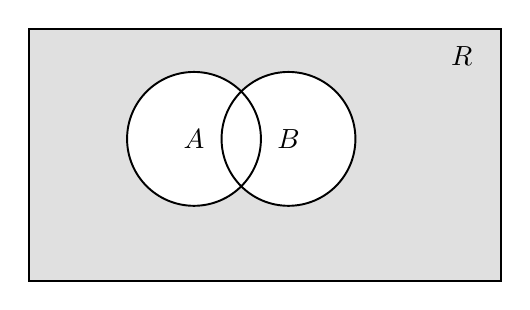
\begin{tikzpicture}[scale=1,line width=0.7pt]
\fill[black!12] (0,0) rectangle (6,3.2);
\fill[white] (2.1,1.8) circle (0.85);
\fill[white] (3.3,1.8) circle (0.85);
\draw (0,0) rectangle (6,3.2);
\draw (2.1,1.8) circle (0.85);
\draw (3.3,1.8) circle (0.85);
\node at (2.1,1.8) {$A$};
\node at (3.3,1.8) {$B$};
\node at (5.5,2.85) {$R$};
\end{tikzpicture}
\end{center}

（1）若集合 $C$ 表示图中阴影部分，用集合的运算式表示 $C$.

（2）求集合 $C$.

\ansspace*[12]

\ifanswer
\solbegin
\stepm{（1）}{由韦恩图得 $C=\overline{A\cup B}$.}
\stepm{（2）}{解 $\dfrac{x+1}{x-2}<-1$，则 $\dfrac{x+1}{x-2}+1<0$，即 $\dfrac{2x-1}{x-2}<0$，解得 $\dfrac12<x<2$，}
\step{故 $B=\left\{x\left|\dfrac12<x<2\right.\right\}$，所以 $A\cup B=\{x\mid-3\leqslant x<2\}$，}
\step{所以 $C=\overline{A\cup B}=\{x\mid x<-3\ \text{或}\ x\geqslant2\}$.}
\solend
\fi

\item 已知集合 $A=\{x\mid x^2-6x+8<0\}$，集合 $B=\{x\mid3m<x<1-m\}$.

（1）命题 $p:x\in A$，命题 $q:x\in B$，若 $p$ 是 $q$ 的充分条件，求实数 $m$ 的取值范围.

（2）若 $A\cap B=\varnothing$，求实数 $m$ 的取值范围.

\ansspace*[12]

\ifanswer
\solbegin
\stepm{（1）}{$x^2-6x+8<0\Rightarrow2<x<4\Rightarrow A=\{x\mid2<x<4\}$.}
\step{若 $p$ 是 $q$ 的充分条件，则 $A\subseteq B$，结合 $B$ 为非空集合，得 $\begin{cases}3m<1-m\\ 3m\leqslant2\\ 1-m\geqslant4\end{cases}$，}
\step{解得 $m\leqslant-3$，故 $m$ 的取值范围是 $(-\infty,-3]$；}
\stepm{（2）}{当 $B=\varnothing$ 时，$3m\geqslant1-m$，解得 $m\geqslant\dfrac14$，满足 $A\cap B=\varnothing$；}
\step{当 $B\neq\varnothing$ 时，$3m<1-m$ 即 $m<\dfrac14$，}
\step{要使交集为空，则 $1-m\leqslant2$ 或 $3m\geqslant4$，解得 $m\geqslant-1$，}
\step{结合 $m<\dfrac14$，得 $-1\leqslant m<\dfrac14$.}
\step{综上，$m\geqslant-1$，即 $m$ 的取值范围是 $[-1,+\infty)$.}
\solend
\fi

\item 设某企业每月生产电机 $x$ 台，根据企业月度报表知，每月总产值 $m$（万元）与总支出 $n$（万元）近似地满足下列关系：$m=\dfrac92x-\dfrac14$，$n=-\dfrac14x^2+5x+\dfrac74$，当 $m-n\geqslant0$ 时，称不亏损企业；当 $m-n<0$ 时，称亏损企业，且 $n-m$ 为亏损额.

（1）企业要成为不亏损企业，每月至少要生产多少台电机？

（2）当月总产值为多少时，企业亏损最严重，最大亏损额为多少？

\ansspace*[12]

\ifanswer
\solbegin
\stepm{（1）}{由题意得 $m-n\geqslant0$，即 $\dfrac92x-\dfrac14\geqslant-\dfrac14x^2+5x+\dfrac74$，}
\step{整理得 $x^2-2x-8\geqslant0$，解得 $x\geqslant4$ 或 $x\leqslant-2$（舍），}
\step{所以企业要成为不亏损企业，每月至少要生产 $4$ 台电机；}
\stepm{（2）}{由（1）得当 $0<x<4$ 时企业亏损，}
\step{亏损额 $n-m=\left(-\dfrac14x^2+5x+\dfrac74\right)-\left(\dfrac92x-\dfrac14\right)=-\dfrac14(x-1)^2+\dfrac94$，}
\step{所以当 $x=1$ 时，$n-m$ 取最大值 $\dfrac94$，}
\step{答：当月总产值为 $1$ 台时，企业亏损最严重，最大亏损额为 $\dfrac94$ 万元.}
\solend
\fi

\item 已知 $x_1$、$x_2$ 是一元二次方程 $4kx^2-4kx+k+1=0(k\neq0)$ 的两个实数根.

（1）是否存在实数 $k$，使 $x_1^2+x_2^2=\dfrac14$ 成立？若存在，求出 $k$ 的值，若不存在，请说明理由；

（2）是否存在整数 $k$，使 $\dfrac{x_1}{x_2}+\dfrac{x_2}{x_1}-2$ 的值为整数？若存在，求出 $k$ 的值，若不存在，请说明理由.

\ansspace*[14]

\ifanswer
\solbegin
\stepm{（1）}{因为 $x_1$、$x_2$ 是一元二次方程 $4kx^2-4kx+k+1=0(k\neq0)$ 的两个实数根，}
\step{所以 $\Delta=(-4k)^2-4\times4k(k+1)\geqslant0$，解得 $k\leqslant0$，}
\step{由韦达定理得 $\begin{cases}x_1+x_2=1\\ x_1x_2=\dfrac{k+1}{4k}\end{cases}$，}
\step{则 $x_1^2+x_2^2=(x_1+x_2)^2-2x_1x_2=\dfrac14$，}
\step{即 $1-2\times\dfrac{k+1}{4k}=\dfrac14$，解得 $k=2$，因为 $k\leqslant0$，所以不存在实数 $k$.}
\stepm{（2）}{$\dfrac{x_1}{x_2}+\dfrac{x_2}{x_1}-2=\dfrac{x_1^2+x_2^2}{x_1x_2}-2=\dfrac{(x_1+x_2)^2-2x_1x_2}{x_1x_2}-2=\dfrac{(x_1+x_2)^2}{x_1x_2}-4$}
\step{$=\dfrac{1}{\dfrac{k+1}{4k}}-4=\dfrac{4k}{k+1}-4=\dfrac{4k-4(k+1)}{k+1}=\dfrac{-4}{k+1}$，}
\step{由于 $\dfrac{x_1}{x_2}+\dfrac{x_2}{x_1}-2$ 的值为整数，即 $\dfrac{-4}{k+1}$ 的值为整数，}
\step{所以 $k+1$ 只能取 $\pm1$、$\pm2$、$\pm4$，}
\step{又 $k\leqslant0$，所以当 $k+1=\pm1$ 时，得出 $k=0$（舍）或 $k=-2$，}
\step{当 $k+1=\pm2$ 时，得出 $k=1$（舍）或 $k=-3$，}
\step{当 $k+1=\pm4$ 时，得出 $k=3$（舍）或 $k=-5$，}
\step{综上所述，若 $\dfrac{x_1}{x_2}+\dfrac{x_2}{x_1}-2$ 的值为整数，则 $k$ 的值为 $-2$ 或 $-3$ 或 $-5$.}
\solend
\fi

\item 已知集合 $A=\{a_1,a_2,\cdots,a_n\}(n\geqslant3)$，其中 $a_m\in\Z(m=1,2,\cdots,n)$. 若 $A$ 的子集 $T=\{a_i,a_j,a_k\}$ 满足 $2a_k=a_i+a_j$，则称 $T$ 具有性质 $P$. $A$ 的所有具有性质 $P$ 的子集 $T$ 的个数记为 $card_A(T)$.

（1）当 $A=\{4,-1,-2,1,-5\}$ 时，写出 $A$ 的所有具有性质 $P$ 的子集 $T$；

（2）当 $n=4$ 时，若 $a_1<a_2<a_3<a_4$，且 $card_A(T)=2$，证明：数对 $a_1$、$a_3$ 和 $a_2$、$a_4$ 中至少有一对中的两数奇偶性相同；

（3）当 $n=9$ 时，求 $card_A(T)$ 的最大值.

\ansspace*[14]

\ifanswer
\solbegin
\stepm{（1）}{集合 $A=\{4,-1,-2,1,-5\}$，元素按从小到大排列为 $-5$、$-2$、$-1$、$1$、$4$，}
\step{满足 $2a_k=a_i+a_j$ 的三元子集 $T$ 需满足其中一个元素是另外两个的平均数，}
\step{对于 $-5,-2,1$：$2\times(-2)=-4=-5+1$，满足条件，故 $T=\{-5,-2,1\}$，}
\step{对于 $-2,1,4$：$2\times1=2=-2+4$，满足条件，故 $T=\{-2,1,4\}$，}
\step{因此满足的子集有 $\{-5,-2,1\}$ 和 $\{-2,1,4\}$.}
\stepm{（2）}{假设数对 $(a_1,a_3)$ 和 $(a_2,a_4)$ 的两数奇偶性均不同，}
\step{即 $a_1$ 与 $a_3$ 一奇一偶，故 $a_1+a_3$ 为奇数，}
\step{$a_2$ 与 $a_4$ 一奇一偶，故 $a_2+a_4$ 为奇数，}
\step{集合 $A=\{a_1,a_2,a_3,a_4\}$ 的三元子集共 $\mathrm{C}_4^3=4$ 个：}
\step{$\{a_1,a_2,a_3\}$：若满足 $2a_2=a_1+a_3$，左边为偶数，右边为奇数，矛盾，故不满足；}
\step{$\{a_2,a_3,a_4\}$：若满足 $2a_3=a_2+a_4$，左边为偶数，右边为奇数，矛盾，故不满足；}
\step{$\{a_1,a_2,a_4\}$：需 $2a_2=a_1+a_4$；}
\step{$\{a_1,a_3,a_4\}$：需 $2a_3=a_1+a_4$.}
\step{若这两个子集都满足，则 $2a_2=2a_3\Rightarrow a_2=a_3$，与 $a_2<a_3$ 矛盾，}
\step{因此最多只有 $1$ 个子集满足条件，与 $card_A(T)=2$ 矛盾，故假设不成立，}
\step{即数对 $(a_1,a_3)$ 和 $(a_2,a_4)$ 中至少有一对的两数奇偶性相同.}
\stepm{（3）}{要最大化 $card_A(T)$，}
\step{集合 $A$ 应包含尽可能多的三元等差数列（即长度为 $3$ 的等差数列），}
\step{当 $A$ 为公差为 $1$ 的等差数列（如 $A=\{0,1,2,\cdots,8\}$）时，}
\step{三元等差数列的个数最多，}
\step{对于集合 $\{0,1,2,\cdots,8\}$，计算三元等差数列个数：}
\step{公差 $d=1$：$\{0,1,2\},\{1,2,3\},\cdots,\{6,7,8\}$，共 $7$ 个；}
\step{公差 $d=2$：$\{0,2,4\},\{1,3,5\},\cdots,\{4,6,8\}$，共 $5$ 个；}
\step{公差 $d=3$：$\{0,3,6\},\{1,4,7\},\{2,5,8\}$，共 $3$ 个；}
\step{公差 $d=4$：$\{0,4,8\}$，共 $1$ 个；}
\step{总个数为 $7+5+3+1=16$.}
\solend
\fi

\end{enumerate}

\end{document}
"
% 紧凑版：xelatex "\def\iscompact{1}% 高一89_宝山中学_10月月考.tex
%   —— 高一上数学“2026-2027 年宝山中学高一上 10 月月考”（讲评版）
% 试卷版：xelatex 高一89_宝山中学_10月月考.tex
% 答案版：xelatex "\def\isanswer{1}\input{高一89_宝山中学_10月月考.tex}"
% 紧凑版：xelatex "\def\iscompact{1}\input{高一89_宝山中学_10月月考.tex}"
%
% 原始材料：微信公众号“魔都数学加油站”文章，连载“27学年高一89”；
% 原文标题“27学年高一89——2026-2027年上海市宝山中学高一上10月月考”；
% 原文链接：https://mp.weixin.qq.com/s/DZ-Q-hfS4UulNW_vGWrZXw。
% 正文为 10 张 PNG 页（`原图/高一89_宝山中学_10月月考/01..10.png`），
% 尺寸混排（第 6 页为 2560×3620，其余为 4762×6735），均按页序读取。
%
% 篇幅与题号：原卷自第 3 题起编号（第 1、2 题不在原文内）。填空题 3—12（10 题）、
% 选择题 13—16（4 题）、解答题 17—21（5 题），共 19 题。
%
% 讲评版：第 4 题只印【答案】（“$x\leqslant2$ 或 $y\leqslant2$”），本稿只给 \ans{}；
% 其余 18 题印【解析】，其中选择题答案在解析末句“故选 C／B／A／A”。
% 第 17 题题干带一幅韦恩图（全集 $R$、集合 $A$、$B$ 与阴影部分），三版都出。
%
% 副标题：原卷未印副标题。本稿按内容标作“集合与常用逻辑用语、不等式”。
%
% 原卷笔误/存疑（均照录未改，正文对应处另有 % 注）：
%   ① 第 8 题题干“$k\in R$”与第 12 题“$n\in N$”按原卷用斜体字母排，本稿沿用
%      $\R$、$\N$ 记号（见“排版差异”③），此处不再视为笔误；
%   ② 第 9 题解析“故 $a$ 的取值范围是 $a<-1$ 或 $\dfrac13<a<\dfrac12$”，未把
%      $a<-1$ 写成区间，与同题前两行的写法不统一，属原卷写法，照录；
%   ③ 第 20 题 (1) 由 $\Delta\geqslant0$ 得“$k\leqslant0$”，与题设 $k\neq0$ 合看
%      应为 $k<0$；原卷写 $k\leqslant0$ 并以之舍去 $k=2$，结论不变，照录。
%
% 与原卷的排版差异：
%   ① 原卷每题下直接印【答案】/【解析】，本稿按全稿惯例将答案与解析置于答案版；
%   ② 原卷未印副标题，本稿补出；填空横线统一排 \blankline[4.4em]；
%   ③ 原卷数集记号排斜体 $R$、$Z$、$N$，本稿按全稿惯例改用 $\R$、$\Z$、$\N$；
%   ④ 第 17—21 题的子问用行内“（1）（2）（3）”段，解析中的子问标号用 \stepm；
%   ⑤ 解答题按惯例加 \ansspace；选择题括号排 \mbox{（\quad）}；
%   ⑥ 第 17 题的韦恩图原卷排在题干右侧、文字绕排，本稿改排为题干后的居中图
%      （TikZ 重绘：原图该处有公众号粉色水印斜压，按原图布局重绘，标注一致）。
%
% 行数核对：逐题数 \step/\stepm 条数，合计 119 条（Q3：2；Q4：0；Q5：3；Q6：4；
% Q7：2；Q8：3；Q9：4；Q10：5；Q11：8；Q12：4；Q13：5；Q14：7；Q15：9；Q16：5；
% Q17：4；Q18：8；Q19：7；Q20：13；Q21：26）。第 4 题只印【答案】，不计入 \step 账。
% 原卷解析的换行按语意合并，未逐行强拆。
%
\documentclass[a4paper,11pt]{article}
\usepackage{common}

\begin{document}

\examtitlest[7]{2026--2027 年宝山中学高一上 10 月月考}{集合与常用逻辑用语、不等式}

\bigsec{一、填空题}

\begin{enumerate}
\setcounter{enumi}{2}

\item 满足 $\{1,2\}\subseteq A\subseteq\{1,2,3,4,5\}$ 的集合共 $A$ 有\blankline[4.4em]个.

\ifanswer
\solbegin
\step{由题意得 $A=\{1,2\}$ 与 $\{3,4,5\}$ 的非空子集的并集，}
\step{而 $\{3,4,5\}$ 的子集有 $2^3=8$ 个，所以满足条件的 $A$ 有 $8$ 个.}
\solend
\fi

\item 用反证法证明命题：“若 $x+y>4$，则 $x>2$ 且 $y>2$”时，第一步应该假设\blankline[4.4em].

\ifanswer
\ans{$x\leqslant2$ 或 $y\leqslant2$}
\fi

\item 已知等式 $2x^2+3x+5=a(2x+1)(x+1)+c$ 恒成立，则 $a-c$ 的值为\blankline[4.4em].

\ifanswer
\solbegin
\step{因为 $2x^2+3x+5=a(2x+1)(x+1)+c$ 恒成立，}
\step{所以 $2x^2+3x+5=2ax^2+3ax+a+c$ 恒成立，}
\step{则 $\begin{cases}2=2a\\ 3=3a\\ 5=a+c\end{cases}$，得 $a=1$，$c=4$，所以 $a-c=-3$.}
\solend
\fi

\item 不等式 $\lvert3x-1\rvert<x$ 的解集\blankline[4.4em].

\ifanswer
\solbegin
\step{当 $x\leqslant0$ 时，不等式的解集为 $\varnothing$，}
\step{当 $x>0$ 时，$\lvert3x-1\rvert<x$，即 $(3x-1)^2<x^2$，}
\step{整理得 $8x^2-6x+1<0$，$(2x-1)(4x-1)<0$，解得 $\dfrac14<x<\dfrac12$，满足 $x>0$.}
\step{故解集为 $\left(\dfrac14,\dfrac12\right)$.}
\solend
\fi

\item 比较两个代数式的大小关系：$x^2+2y^2$\blankline[3em]$2xy+2y-1$.

\ifanswer
\solbegin
\step{$x^2+2y^2-(2xy+2y-1)=x^2-2xy+y^2+y^2-2y+1$}
\step{$=(x-y)^2+(y-1)^2\geqslant0$，所以 $x^2+2y^2\geqslant2xy+2y-1$.}
\solend
\fi

\item $k\in\R$，关于 $x$ 的不等式 $x^2+\sqrt2kx+2>0$ 的解集为全体实数，则 $k$ 的取值范围是\blankline[4.4em].

\ifanswer
\solbegin
\step{因为关于 $x$ 的不等式 $x^2+\sqrt2kx+2>0$ 的解集为全体实数，}
\step{所以 $\Delta=(\sqrt2k)^2-4\times1\times2=2k^2-8<0$，解得 $-2<k<2$，}
\step{即实数 $k$ 的取值范围是 $(-2,2)$.}
\solend
\fi

\item 在平面直角坐标系内，点 $\left(2a-1,\dfrac{3a-1}{a+1}\right)$ 在第二象限，则 $a$ 的取值范围是\blankline[4.4em].

\ifanswer
\solbegin
\step{由题意得 $\begin{cases}2a-1<0\\[0.2em]\dfrac{3a-1}{a+1}>0\end{cases}$，}
\step{由 $2a-1<0$，解得 $a<\dfrac12$；}
\step{由 $\dfrac{3a-1}{a+1}>0$，解得 $a<-1$ 或 $a>\dfrac13$；}
\step{故 $a$ 的取值范围是 $a<-1$ 或 $\dfrac13<a<\dfrac12$.}
\solend
\fi

\item 设集合 $A=\{x\mid x^2+x-6=0\}$，集合 $B=\{x\mid mx+1=0\}$，且 $A\cup B=A$，则 $m$ 的值组成的集合是\blankline[4.4em].

\ifanswer
\solbegin
\step{由题意得 $A=\{x\mid x^2+x-6=0\}=\{-3,2\}$，}
\step{由 $A\cup B=A$，得 $B\subseteq A$，}
\step{当 $m=0$ 时，$B=\varnothing$，满足题意，}
\step{当 $m\neq0$ 时，$B=\left\{-\dfrac1m\right\}$，所以 $-\dfrac1m=2$ 或 $-\dfrac1m=-3$，所以 $m=-\dfrac12$ 或 $m=\dfrac13$，}
\step{综上所述，$m$ 的值组成的集合是 $\left\{0,-\dfrac12,\dfrac13\right\}$.}
\solend
\fi

\item 甲、乙两人解关于 $x$ 的不等式 $x^2+bx+c<0$，甲写错了 $b$，正确计算后得到的解为 $\{x\mid1<x<2\}$；乙写错了 $c$，正确计算后得到的解为 $\{x\mid-4<x<1\}$. 那么不等式 $\dfrac{bx+c}{x-2}<0$ 的解为\blankline[4.4em].

\ifanswer
\solbegin
\step{由 $x^2+bx+c<0$ 的解为 $\{x\mid1<x<2\}$，}
\step{则 $1$ 和 $2$ 是方程 $x^2+bx+c=0$ 的两个根，}
\step{甲写错了 $b$，但 $c$ 是正确的，所以 $c=1\times2=2$；}
\step{由 $x^2+bx+c<0$ 的解为 $\{x\mid-4<x<1\}$，}
\step{则 $-4$ 和 $1$ 是方程 $x^2+bx+c=0$ 的两个根，}
\step{乙写错了 $c$，但 $b$ 是正确的，所以 $-b=-4+1=-3$，即 $b=3$.}
\step{由 $\dfrac{bx+c}{x-2}<0$，得 $\dfrac{3x+2}{x-2}<0$，即 $(3x+2)(x-2)<0$，解得 $-\dfrac23<x<2$，}
\step{所以不等式 $\dfrac{bx+c}{x-2}<0$ 的解为 $\left\{x\left|-\dfrac23<x<2\right.\right\}$.}
\solend
\fi

\item 已知集合 $M$ 的元素均为正整数，定义集合 $M$ 的“变项和”为：将 $M$ 中每个元素 $m$ 都乘以 $(-1)^m$ 后再求和. 若集合 $A=\{n\mid1\leqslant n\leqslant10,n\in\N\}$，则集合 $A$ 的所有非空子集的“变项和”的总和为\blankline[4.4em].

\ifanswer
\solbegin
\step{$A$ 集合的所有非空子集中，每个元素出现的次数都是 $(2^{10}-1)-(2^9-1)=2^9$，}
\step{则集合 $A$ 的所有非空子集的“变项和”的总和}
\step{为 $1\times(-1)^1\times2^9+2\times(-1)^2\times2^9+\cdots+10\times(-1)^{10}\times2^9$}
\step{$=(-1+2-3+4-\cdots-9+10)\times2^9=5\times2^9=2560$.}
\solend
\fi

\end{enumerate}

\bigsec{二、选择题}

\begin{enumerate}
\setcounter{enumi}{12}

\item 下列命题中正确的是\mbox{（\quad）}

\keepwithprev
A. 若 $a>b$，则 $\dfrac1a<\dfrac1b$\qquad B. 若 $a>b$，则 $a^2>b^2$

C. 若 $a>\lvert b\rvert$，则 $a>b$\qquad D. 若 $a>b$，则 $ac^2>bc^2$

\ifanswer
\solbegin
\step{对于 $AB$ 选项，取 $a=1$，$b=-1$，$a>b$，$\dfrac1a>\dfrac1b$，$a^2=b^2$，}
\step{所以 $AB$ 选项错误；}
\step{对于 $C$ 选项，由 $a>\lvert b\rvert$，$\lvert b\rvert\geqslant b$，得 $a>b$，所以 $C$ 选项正确；}
\step{对于 $D$ 选项，取 $c=0$，则 $ac^2=0=bc^2$，所以 $D$ 选项错误.}
\step{故选 $C$.}
\solend
\fi

\item 下面关于集合的表示正确的个数是\mbox{（\quad）}

①$\{1,2,3\}=\{3,2,1\}$；\quad ②$\{(x,y)\mid x-y=1\}=\{y\mid y=x-1\}$；

③$\{x\mid x\geqslant2,x\in\N\}=\{y\mid y\geqslant2,y\in\Z\}$；\quad ④$\{x\mid x+2y=1\}\neq\left\{y\left|y=-\dfrac12x+\dfrac12\right.\right\}$.

\keepwithprev
A. $1$\qquad B. $2$\qquad C. $3$\qquad D. $4$

\ifanswer
\solbegin
\step{对于①，由元素的无序性得①正确；}
\step{对于②，$\{(x,y)\mid x-y=1\}$ 表示点集，$\{y\mid y=x-1\}$ 表示数集，故②错误；}
\step{对于③，$\{x\mid x\geqslant2,x\in\N\}$ 表示大于等于 $2$ 的整数，}
\step{$\{y\mid y\geqslant2,y\in\Z\}$ 也表示大于等于 $2$ 的整数，故③正确；}
\step{对于④，$\{x\mid x+2y=1\}=\R$，$\left\{y\left|y=-\dfrac12x+\dfrac12\right.\right\}=\R$，}
\step{所以 $\{x\mid x+2y=1\}=\left\{y\left|y=-\dfrac12x+\dfrac12\right.\right\}$，故④错误，}
\step{所以正确的个数是 $2$ 个. 故选 $B$.}
\solend
\fi

\item 已知命题 $P$：方程 $ax^2+bx+c=0$ 有两个不相等实根；命题 $Q$：不等式 $ax^2+bx+c>0$ 与 $ax^2+bx+c<0$ 均有解，则命题 $P$ 成立是命题 $Q$ 成立的\mbox{（\quad）}条件.

\keepwithprev
A. 充分非必要条件\qquad B. 必要非充分条件

C. 充要条件\qquad D. 既非充分又非必要条件

\ifanswer
\solbegin
\step{若 $P$ 成立，即方程 $ax^2+bx+c=0$ 有两个不相等实根，}
\step{此时 $\begin{cases}a\neq0\\ \Delta=b^2-4ac>0\end{cases}$；}
\step{若 $Q$ 成立，即不等式 $ax^2+bx+c>0$ 与 $ax^2+bx+c<0$ 均有解，有两种情况：}
\step{①不等式是一元二次不等式，}
\step{此时不等式所对应的二次函数的图像与 $x$ 轴有两个交点，}
\step{满足 $\begin{cases}a\neq0\\ \Delta=b^2-4ac>0\end{cases}$；}
\step{②不等式是一元一次不等式，此时 $\begin{cases}a=0\\ b\neq0\end{cases}$，}
\step{因此，由 $P$ 能推出 $Q$ 成立，但是由 $Q$ 不能推出 $P$ 成立，}
\step{即 $P$ 是 $Q$ 的充分非必要条件. 故选 $A$.}
\solend
\fi

\item 甲、乙同去加油站加油两次，两次汽油单价分别为 $x$、$y$ 元/升（$x\neq y$）. 甲每次加固定金额的油，乙每次加固定体积的油. 哪种方式更经济实惠呢？\mbox{（\quad）}

\keepwithprev
A. 加固定金额的方式\qquad B. 加固定体积的方式

C. 两种方案一样\qquad D. 要视具体价格而定

\ifanswer
\solbegin
\step{设两次加油的油价分别为 $x$、$y$（$x$、$y>0$，且 $x\neq y$），}
\step{乙每次加油的量为 $a$（$a>0$）；甲每次加油的钱数为 $b$（$b>0$），}
\step{则乙平均油价为 $\dfrac{ax+ay}{2a}=\dfrac{x+y}{2}$，甲平均油价为 $\dfrac{2b}{\dfrac bx+\dfrac by}=\dfrac2{\dfrac1x+\dfrac1y}=\dfrac{2xy}{x+y}$，}
\step{因为 $x\neq y$，所以 $\dfrac{x+y}{2}-\dfrac{2xy}{x+y}=\dfrac{(x-y)^2}{2(x+y)}>0$，所以 $\dfrac{x+y}{2}>\dfrac{2xy}{x+y}$，}
\step{即甲方案更经济. 故选 $A$.}
\solend
\fi

\end{enumerate}

\bigsec{三、解答题}

\begin{enumerate}
\setcounter{enumi}{16}

\item 已知全集 $U=\R$，集合 $A=\{x\mid-3\leqslant x\leqslant1\}$，$B=\left\{x\left|\dfrac{x+1}{x-2}<-1\right.\right\}$.

\begin{center}
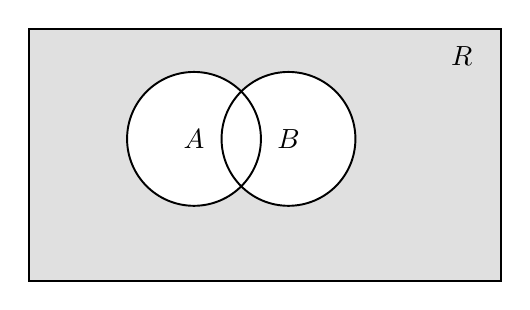
\begin{tikzpicture}[scale=1,line width=0.7pt]
\fill[black!12] (0,0) rectangle (6,3.2);
\fill[white] (2.1,1.8) circle (0.85);
\fill[white] (3.3,1.8) circle (0.85);
\draw (0,0) rectangle (6,3.2);
\draw (2.1,1.8) circle (0.85);
\draw (3.3,1.8) circle (0.85);
\node at (2.1,1.8) {$A$};
\node at (3.3,1.8) {$B$};
\node at (5.5,2.85) {$R$};
\end{tikzpicture}
\end{center}

（1）若集合 $C$ 表示图中阴影部分，用集合的运算式表示 $C$.

（2）求集合 $C$.

\ansspace*[12]

\ifanswer
\solbegin
\stepm{（1）}{由韦恩图得 $C=\overline{A\cup B}$.}
\stepm{（2）}{解 $\dfrac{x+1}{x-2}<-1$，则 $\dfrac{x+1}{x-2}+1<0$，即 $\dfrac{2x-1}{x-2}<0$，解得 $\dfrac12<x<2$，}
\step{故 $B=\left\{x\left|\dfrac12<x<2\right.\right\}$，所以 $A\cup B=\{x\mid-3\leqslant x<2\}$，}
\step{所以 $C=\overline{A\cup B}=\{x\mid x<-3\ \text{或}\ x\geqslant2\}$.}
\solend
\fi

\item 已知集合 $A=\{x\mid x^2-6x+8<0\}$，集合 $B=\{x\mid3m<x<1-m\}$.

（1）命题 $p:x\in A$，命题 $q:x\in B$，若 $p$ 是 $q$ 的充分条件，求实数 $m$ 的取值范围.

（2）若 $A\cap B=\varnothing$，求实数 $m$ 的取值范围.

\ansspace*[12]

\ifanswer
\solbegin
\stepm{（1）}{$x^2-6x+8<0\Rightarrow2<x<4\Rightarrow A=\{x\mid2<x<4\}$.}
\step{若 $p$ 是 $q$ 的充分条件，则 $A\subseteq B$，结合 $B$ 为非空集合，得 $\begin{cases}3m<1-m\\ 3m\leqslant2\\ 1-m\geqslant4\end{cases}$，}
\step{解得 $m\leqslant-3$，故 $m$ 的取值范围是 $(-\infty,-3]$；}
\stepm{（2）}{当 $B=\varnothing$ 时，$3m\geqslant1-m$，解得 $m\geqslant\dfrac14$，满足 $A\cap B=\varnothing$；}
\step{当 $B\neq\varnothing$ 时，$3m<1-m$ 即 $m<\dfrac14$，}
\step{要使交集为空，则 $1-m\leqslant2$ 或 $3m\geqslant4$，解得 $m\geqslant-1$，}
\step{结合 $m<\dfrac14$，得 $-1\leqslant m<\dfrac14$.}
\step{综上，$m\geqslant-1$，即 $m$ 的取值范围是 $[-1,+\infty)$.}
\solend
\fi

\item 设某企业每月生产电机 $x$ 台，根据企业月度报表知，每月总产值 $m$（万元）与总支出 $n$（万元）近似地满足下列关系：$m=\dfrac92x-\dfrac14$，$n=-\dfrac14x^2+5x+\dfrac74$，当 $m-n\geqslant0$ 时，称不亏损企业；当 $m-n<0$ 时，称亏损企业，且 $n-m$ 为亏损额.

（1）企业要成为不亏损企业，每月至少要生产多少台电机？

（2）当月总产值为多少时，企业亏损最严重，最大亏损额为多少？

\ansspace*[12]

\ifanswer
\solbegin
\stepm{（1）}{由题意得 $m-n\geqslant0$，即 $\dfrac92x-\dfrac14\geqslant-\dfrac14x^2+5x+\dfrac74$，}
\step{整理得 $x^2-2x-8\geqslant0$，解得 $x\geqslant4$ 或 $x\leqslant-2$（舍），}
\step{所以企业要成为不亏损企业，每月至少要生产 $4$ 台电机；}
\stepm{（2）}{由（1）得当 $0<x<4$ 时企业亏损，}
\step{亏损额 $n-m=\left(-\dfrac14x^2+5x+\dfrac74\right)-\left(\dfrac92x-\dfrac14\right)=-\dfrac14(x-1)^2+\dfrac94$，}
\step{所以当 $x=1$ 时，$n-m$ 取最大值 $\dfrac94$，}
\step{答：当月总产值为 $1$ 台时，企业亏损最严重，最大亏损额为 $\dfrac94$ 万元.}
\solend
\fi

\item 已知 $x_1$、$x_2$ 是一元二次方程 $4kx^2-4kx+k+1=0(k\neq0)$ 的两个实数根.

（1）是否存在实数 $k$，使 $x_1^2+x_2^2=\dfrac14$ 成立？若存在，求出 $k$ 的值，若不存在，请说明理由；

（2）是否存在整数 $k$，使 $\dfrac{x_1}{x_2}+\dfrac{x_2}{x_1}-2$ 的值为整数？若存在，求出 $k$ 的值，若不存在，请说明理由.

\ansspace*[14]

\ifanswer
\solbegin
\stepm{（1）}{因为 $x_1$、$x_2$ 是一元二次方程 $4kx^2-4kx+k+1=0(k\neq0)$ 的两个实数根，}
\step{所以 $\Delta=(-4k)^2-4\times4k(k+1)\geqslant0$，解得 $k\leqslant0$，}
\step{由韦达定理得 $\begin{cases}x_1+x_2=1\\ x_1x_2=\dfrac{k+1}{4k}\end{cases}$，}
\step{则 $x_1^2+x_2^2=(x_1+x_2)^2-2x_1x_2=\dfrac14$，}
\step{即 $1-2\times\dfrac{k+1}{4k}=\dfrac14$，解得 $k=2$，因为 $k\leqslant0$，所以不存在实数 $k$.}
\stepm{（2）}{$\dfrac{x_1}{x_2}+\dfrac{x_2}{x_1}-2=\dfrac{x_1^2+x_2^2}{x_1x_2}-2=\dfrac{(x_1+x_2)^2-2x_1x_2}{x_1x_2}-2=\dfrac{(x_1+x_2)^2}{x_1x_2}-4$}
\step{$=\dfrac{1}{\dfrac{k+1}{4k}}-4=\dfrac{4k}{k+1}-4=\dfrac{4k-4(k+1)}{k+1}=\dfrac{-4}{k+1}$，}
\step{由于 $\dfrac{x_1}{x_2}+\dfrac{x_2}{x_1}-2$ 的值为整数，即 $\dfrac{-4}{k+1}$ 的值为整数，}
\step{所以 $k+1$ 只能取 $\pm1$、$\pm2$、$\pm4$，}
\step{又 $k\leqslant0$，所以当 $k+1=\pm1$ 时，得出 $k=0$（舍）或 $k=-2$，}
\step{当 $k+1=\pm2$ 时，得出 $k=1$（舍）或 $k=-3$，}
\step{当 $k+1=\pm4$ 时，得出 $k=3$（舍）或 $k=-5$，}
\step{综上所述，若 $\dfrac{x_1}{x_2}+\dfrac{x_2}{x_1}-2$ 的值为整数，则 $k$ 的值为 $-2$ 或 $-3$ 或 $-5$.}
\solend
\fi

\item 已知集合 $A=\{a_1,a_2,\cdots,a_n\}(n\geqslant3)$，其中 $a_m\in\Z(m=1,2,\cdots,n)$. 若 $A$ 的子集 $T=\{a_i,a_j,a_k\}$ 满足 $2a_k=a_i+a_j$，则称 $T$ 具有性质 $P$. $A$ 的所有具有性质 $P$ 的子集 $T$ 的个数记为 $card_A(T)$.

（1）当 $A=\{4,-1,-2,1,-5\}$ 时，写出 $A$ 的所有具有性质 $P$ 的子集 $T$；

（2）当 $n=4$ 时，若 $a_1<a_2<a_3<a_4$，且 $card_A(T)=2$，证明：数对 $a_1$、$a_3$ 和 $a_2$、$a_4$ 中至少有一对中的两数奇偶性相同；

（3）当 $n=9$ 时，求 $card_A(T)$ 的最大值.

\ansspace*[14]

\ifanswer
\solbegin
\stepm{（1）}{集合 $A=\{4,-1,-2,1,-5\}$，元素按从小到大排列为 $-5$、$-2$、$-1$、$1$、$4$，}
\step{满足 $2a_k=a_i+a_j$ 的三元子集 $T$ 需满足其中一个元素是另外两个的平均数，}
\step{对于 $-5,-2,1$：$2\times(-2)=-4=-5+1$，满足条件，故 $T=\{-5,-2,1\}$，}
\step{对于 $-2,1,4$：$2\times1=2=-2+4$，满足条件，故 $T=\{-2,1,4\}$，}
\step{因此满足的子集有 $\{-5,-2,1\}$ 和 $\{-2,1,4\}$.}
\stepm{（2）}{假设数对 $(a_1,a_3)$ 和 $(a_2,a_4)$ 的两数奇偶性均不同，}
\step{即 $a_1$ 与 $a_3$ 一奇一偶，故 $a_1+a_3$ 为奇数，}
\step{$a_2$ 与 $a_4$ 一奇一偶，故 $a_2+a_4$ 为奇数，}
\step{集合 $A=\{a_1,a_2,a_3,a_4\}$ 的三元子集共 $\mathrm{C}_4^3=4$ 个：}
\step{$\{a_1,a_2,a_3\}$：若满足 $2a_2=a_1+a_3$，左边为偶数，右边为奇数，矛盾，故不满足；}
\step{$\{a_2,a_3,a_4\}$：若满足 $2a_3=a_2+a_4$，左边为偶数，右边为奇数，矛盾，故不满足；}
\step{$\{a_1,a_2,a_4\}$：需 $2a_2=a_1+a_4$；}
\step{$\{a_1,a_3,a_4\}$：需 $2a_3=a_1+a_4$.}
\step{若这两个子集都满足，则 $2a_2=2a_3\Rightarrow a_2=a_3$，与 $a_2<a_3$ 矛盾，}
\step{因此最多只有 $1$ 个子集满足条件，与 $card_A(T)=2$ 矛盾，故假设不成立，}
\step{即数对 $(a_1,a_3)$ 和 $(a_2,a_4)$ 中至少有一对的两数奇偶性相同.}
\stepm{（3）}{要最大化 $card_A(T)$，}
\step{集合 $A$ 应包含尽可能多的三元等差数列（即长度为 $3$ 的等差数列），}
\step{当 $A$ 为公差为 $1$ 的等差数列（如 $A=\{0,1,2,\cdots,8\}$）时，}
\step{三元等差数列的个数最多，}
\step{对于集合 $\{0,1,2,\cdots,8\}$，计算三元等差数列个数：}
\step{公差 $d=1$：$\{0,1,2\},\{1,2,3\},\cdots,\{6,7,8\}$，共 $7$ 个；}
\step{公差 $d=2$：$\{0,2,4\},\{1,3,5\},\cdots,\{4,6,8\}$，共 $5$ 个；}
\step{公差 $d=3$：$\{0,3,6\},\{1,4,7\},\{2,5,8\}$，共 $3$ 个；}
\step{公差 $d=4$：$\{0,4,8\}$，共 $1$ 个；}
\step{总个数为 $7+5+3+1=16$.}
\solend
\fi

\end{enumerate}

\end{document}
"
%
% 原始材料：微信公众号“魔都数学加油站”文章，连载“27学年高一89”；
% 原文标题“27学年高一89——2026-2027年上海市宝山中学高一上10月月考”；
% 原文链接：https://mp.weixin.qq.com/s/DZ-Q-hfS4UulNW_vGWrZXw。
% 正文为 10 张 PNG 页（`原图/高一89_宝山中学_10月月考/01..10.png`），
% 尺寸混排（第 6 页为 2560×3620，其余为 4762×6735），均按页序读取。
%
% 篇幅与题号：原卷自第 3 题起编号（第 1、2 题不在原文内）。填空题 3—12（10 题）、
% 选择题 13—16（4 题）、解答题 17—21（5 题），共 19 题。
%
% 讲评版：第 4 题只印【答案】（“$x\leqslant2$ 或 $y\leqslant2$”），本稿只给 \ans{}；
% 其余 18 题印【解析】，其中选择题答案在解析末句“故选 C／B／A／A”。
% 第 17 题题干带一幅韦恩图（全集 $R$、集合 $A$、$B$ 与阴影部分），三版都出。
%
% 副标题：原卷未印副标题。本稿按内容标作“集合与常用逻辑用语、不等式”。
%
% 原卷笔误/存疑（均照录未改，正文对应处另有 % 注）：
%   ① 第 8 题题干“$k\in R$”与第 12 题“$n\in N$”按原卷用斜体字母排，本稿沿用
%      $\R$、$\N$ 记号（见“排版差异”③），此处不再视为笔误；
%   ② 第 9 题解析“故 $a$ 的取值范围是 $a<-1$ 或 $\dfrac13<a<\dfrac12$”，未把
%      $a<-1$ 写成区间，与同题前两行的写法不统一，属原卷写法，照录；
%   ③ 第 20 题 (1) 由 $\Delta\geqslant0$ 得“$k\leqslant0$”，与题设 $k\neq0$ 合看
%      应为 $k<0$；原卷写 $k\leqslant0$ 并以之舍去 $k=2$，结论不变，照录。
%
% 与原卷的排版差异：
%   ① 原卷每题下直接印【答案】/【解析】，本稿按全稿惯例将答案与解析置于答案版；
%   ② 原卷未印副标题，本稿补出；填空横线统一排 \blankline[4.4em]；
%   ③ 原卷数集记号排斜体 $R$、$Z$、$N$，本稿按全稿惯例改用 $\R$、$\Z$、$\N$；
%   ④ 第 17—21 题的子问用行内“（1）（2）（3）”段，解析中的子问标号用 \stepm；
%   ⑤ 解答题按惯例加 \ansspace；选择题括号排 \mbox{（\quad）}；
%   ⑥ 第 17 题的韦恩图原卷排在题干右侧、文字绕排，本稿改排为题干后的居中图
%      （TikZ 重绘：原图该处有公众号粉色水印斜压，按原图布局重绘，标注一致）。
%
% 行数核对：逐题数 \step/\stepm 条数，合计 119 条（Q3：2；Q4：0；Q5：3；Q6：4；
% Q7：2；Q8：3；Q9：4；Q10：5；Q11：8；Q12：4；Q13：5；Q14：7；Q15：9；Q16：5；
% Q17：4；Q18：8；Q19：7；Q20：13；Q21：26）。第 4 题只印【答案】，不计入 \step 账。
% 原卷解析的换行按语意合并，未逐行强拆。
%
\documentclass[a4paper,11pt]{article}
\usepackage{common}

\begin{document}

\examtitlest[7]{2026--2027 年宝山中学高一上 10 月月考}{集合与常用逻辑用语、不等式}

\bigsec{一、填空题}

\begin{enumerate}
\setcounter{enumi}{2}

\item 满足 $\{1,2\}\subseteq A\subseteq\{1,2,3,4,5\}$ 的集合共 $A$ 有\blankline[4.4em]个.

\ifanswer
\solbegin
\step{由题意得 $A=\{1,2\}$ 与 $\{3,4,5\}$ 的非空子集的并集，}
\step{而 $\{3,4,5\}$ 的子集有 $2^3=8$ 个，所以满足条件的 $A$ 有 $8$ 个.}
\solend
\fi

\item 用反证法证明命题：“若 $x+y>4$，则 $x>2$ 且 $y>2$”时，第一步应该假设\blankline[4.4em].

\ifanswer
\ans{$x\leqslant2$ 或 $y\leqslant2$}
\fi

\item 已知等式 $2x^2+3x+5=a(2x+1)(x+1)+c$ 恒成立，则 $a-c$ 的值为\blankline[4.4em].

\ifanswer
\solbegin
\step{因为 $2x^2+3x+5=a(2x+1)(x+1)+c$ 恒成立，}
\step{所以 $2x^2+3x+5=2ax^2+3ax+a+c$ 恒成立，}
\step{则 $\begin{cases}2=2a\\ 3=3a\\ 5=a+c\end{cases}$，得 $a=1$，$c=4$，所以 $a-c=-3$.}
\solend
\fi

\item 不等式 $\lvert3x-1\rvert<x$ 的解集\blankline[4.4em].

\ifanswer
\solbegin
\step{当 $x\leqslant0$ 时，不等式的解集为 $\varnothing$，}
\step{当 $x>0$ 时，$\lvert3x-1\rvert<x$，即 $(3x-1)^2<x^2$，}
\step{整理得 $8x^2-6x+1<0$，$(2x-1)(4x-1)<0$，解得 $\dfrac14<x<\dfrac12$，满足 $x>0$.}
\step{故解集为 $\left(\dfrac14,\dfrac12\right)$.}
\solend
\fi

\item 比较两个代数式的大小关系：$x^2+2y^2$\blankline[3em]$2xy+2y-1$.

\ifanswer
\solbegin
\step{$x^2+2y^2-(2xy+2y-1)=x^2-2xy+y^2+y^2-2y+1$}
\step{$=(x-y)^2+(y-1)^2\geqslant0$，所以 $x^2+2y^2\geqslant2xy+2y-1$.}
\solend
\fi

\item $k\in\R$，关于 $x$ 的不等式 $x^2+\sqrt2kx+2>0$ 的解集为全体实数，则 $k$ 的取值范围是\blankline[4.4em].

\ifanswer
\solbegin
\step{因为关于 $x$ 的不等式 $x^2+\sqrt2kx+2>0$ 的解集为全体实数，}
\step{所以 $\Delta=(\sqrt2k)^2-4\times1\times2=2k^2-8<0$，解得 $-2<k<2$，}
\step{即实数 $k$ 的取值范围是 $(-2,2)$.}
\solend
\fi

\item 在平面直角坐标系内，点 $\left(2a-1,\dfrac{3a-1}{a+1}\right)$ 在第二象限，则 $a$ 的取值范围是\blankline[4.4em].

\ifanswer
\solbegin
\step{由题意得 $\begin{cases}2a-1<0\\[0.2em]\dfrac{3a-1}{a+1}>0\end{cases}$，}
\step{由 $2a-1<0$，解得 $a<\dfrac12$；}
\step{由 $\dfrac{3a-1}{a+1}>0$，解得 $a<-1$ 或 $a>\dfrac13$；}
\step{故 $a$ 的取值范围是 $a<-1$ 或 $\dfrac13<a<\dfrac12$.}
\solend
\fi

\item 设集合 $A=\{x\mid x^2+x-6=0\}$，集合 $B=\{x\mid mx+1=0\}$，且 $A\cup B=A$，则 $m$ 的值组成的集合是\blankline[4.4em].

\ifanswer
\solbegin
\step{由题意得 $A=\{x\mid x^2+x-6=0\}=\{-3,2\}$，}
\step{由 $A\cup B=A$，得 $B\subseteq A$，}
\step{当 $m=0$ 时，$B=\varnothing$，满足题意，}
\step{当 $m\neq0$ 时，$B=\left\{-\dfrac1m\right\}$，所以 $-\dfrac1m=2$ 或 $-\dfrac1m=-3$，所以 $m=-\dfrac12$ 或 $m=\dfrac13$，}
\step{综上所述，$m$ 的值组成的集合是 $\left\{0,-\dfrac12,\dfrac13\right\}$.}
\solend
\fi

\item 甲、乙两人解关于 $x$ 的不等式 $x^2+bx+c<0$，甲写错了 $b$，正确计算后得到的解为 $\{x\mid1<x<2\}$；乙写错了 $c$，正确计算后得到的解为 $\{x\mid-4<x<1\}$. 那么不等式 $\dfrac{bx+c}{x-2}<0$ 的解为\blankline[4.4em].

\ifanswer
\solbegin
\step{由 $x^2+bx+c<0$ 的解为 $\{x\mid1<x<2\}$，}
\step{则 $1$ 和 $2$ 是方程 $x^2+bx+c=0$ 的两个根，}
\step{甲写错了 $b$，但 $c$ 是正确的，所以 $c=1\times2=2$；}
\step{由 $x^2+bx+c<0$ 的解为 $\{x\mid-4<x<1\}$，}
\step{则 $-4$ 和 $1$ 是方程 $x^2+bx+c=0$ 的两个根，}
\step{乙写错了 $c$，但 $b$ 是正确的，所以 $-b=-4+1=-3$，即 $b=3$.}
\step{由 $\dfrac{bx+c}{x-2}<0$，得 $\dfrac{3x+2}{x-2}<0$，即 $(3x+2)(x-2)<0$，解得 $-\dfrac23<x<2$，}
\step{所以不等式 $\dfrac{bx+c}{x-2}<0$ 的解为 $\left\{x\left|-\dfrac23<x<2\right.\right\}$.}
\solend
\fi

\item 已知集合 $M$ 的元素均为正整数，定义集合 $M$ 的“变项和”为：将 $M$ 中每个元素 $m$ 都乘以 $(-1)^m$ 后再求和. 若集合 $A=\{n\mid1\leqslant n\leqslant10,n\in\N\}$，则集合 $A$ 的所有非空子集的“变项和”的总和为\blankline[4.4em].

\ifanswer
\solbegin
\step{$A$ 集合的所有非空子集中，每个元素出现的次数都是 $(2^{10}-1)-(2^9-1)=2^9$，}
\step{则集合 $A$ 的所有非空子集的“变项和”的总和}
\step{为 $1\times(-1)^1\times2^9+2\times(-1)^2\times2^9+\cdots+10\times(-1)^{10}\times2^9$}
\step{$=(-1+2-3+4-\cdots-9+10)\times2^9=5\times2^9=2560$.}
\solend
\fi

\end{enumerate}

\bigsec{二、选择题}

\begin{enumerate}
\setcounter{enumi}{12}

\item 下列命题中正确的是\mbox{（\quad）}

\keepwithprev
A. 若 $a>b$，则 $\dfrac1a<\dfrac1b$\qquad B. 若 $a>b$，则 $a^2>b^2$

C. 若 $a>\lvert b\rvert$，则 $a>b$\qquad D. 若 $a>b$，则 $ac^2>bc^2$

\ifanswer
\solbegin
\step{对于 $AB$ 选项，取 $a=1$，$b=-1$，$a>b$，$\dfrac1a>\dfrac1b$，$a^2=b^2$，}
\step{所以 $AB$ 选项错误；}
\step{对于 $C$ 选项，由 $a>\lvert b\rvert$，$\lvert b\rvert\geqslant b$，得 $a>b$，所以 $C$ 选项正确；}
\step{对于 $D$ 选项，取 $c=0$，则 $ac^2=0=bc^2$，所以 $D$ 选项错误.}
\step{故选 $C$.}
\solend
\fi

\item 下面关于集合的表示正确的个数是\mbox{（\quad）}

①$\{1,2,3\}=\{3,2,1\}$；\quad ②$\{(x,y)\mid x-y=1\}=\{y\mid y=x-1\}$；

③$\{x\mid x\geqslant2,x\in\N\}=\{y\mid y\geqslant2,y\in\Z\}$；\quad ④$\{x\mid x+2y=1\}\neq\left\{y\left|y=-\dfrac12x+\dfrac12\right.\right\}$.

\keepwithprev
A. $1$\qquad B. $2$\qquad C. $3$\qquad D. $4$

\ifanswer
\solbegin
\step{对于①，由元素的无序性得①正确；}
\step{对于②，$\{(x,y)\mid x-y=1\}$ 表示点集，$\{y\mid y=x-1\}$ 表示数集，故②错误；}
\step{对于③，$\{x\mid x\geqslant2,x\in\N\}$ 表示大于等于 $2$ 的整数，}
\step{$\{y\mid y\geqslant2,y\in\Z\}$ 也表示大于等于 $2$ 的整数，故③正确；}
\step{对于④，$\{x\mid x+2y=1\}=\R$，$\left\{y\left|y=-\dfrac12x+\dfrac12\right.\right\}=\R$，}
\step{所以 $\{x\mid x+2y=1\}=\left\{y\left|y=-\dfrac12x+\dfrac12\right.\right\}$，故④错误，}
\step{所以正确的个数是 $2$ 个. 故选 $B$.}
\solend
\fi

\item 已知命题 $P$：方程 $ax^2+bx+c=0$ 有两个不相等实根；命题 $Q$：不等式 $ax^2+bx+c>0$ 与 $ax^2+bx+c<0$ 均有解，则命题 $P$ 成立是命题 $Q$ 成立的\mbox{（\quad）}条件.

\keepwithprev
A. 充分非必要条件\qquad B. 必要非充分条件

C. 充要条件\qquad D. 既非充分又非必要条件

\ifanswer
\solbegin
\step{若 $P$ 成立，即方程 $ax^2+bx+c=0$ 有两个不相等实根，}
\step{此时 $\begin{cases}a\neq0\\ \Delta=b^2-4ac>0\end{cases}$；}
\step{若 $Q$ 成立，即不等式 $ax^2+bx+c>0$ 与 $ax^2+bx+c<0$ 均有解，有两种情况：}
\step{①不等式是一元二次不等式，}
\step{此时不等式所对应的二次函数的图像与 $x$ 轴有两个交点，}
\step{满足 $\begin{cases}a\neq0\\ \Delta=b^2-4ac>0\end{cases}$；}
\step{②不等式是一元一次不等式，此时 $\begin{cases}a=0\\ b\neq0\end{cases}$，}
\step{因此，由 $P$ 能推出 $Q$ 成立，但是由 $Q$ 不能推出 $P$ 成立，}
\step{即 $P$ 是 $Q$ 的充分非必要条件. 故选 $A$.}
\solend
\fi

\item 甲、乙同去加油站加油两次，两次汽油单价分别为 $x$、$y$ 元/升（$x\neq y$）. 甲每次加固定金额的油，乙每次加固定体积的油. 哪种方式更经济实惠呢？\mbox{（\quad）}

\keepwithprev
A. 加固定金额的方式\qquad B. 加固定体积的方式

C. 两种方案一样\qquad D. 要视具体价格而定

\ifanswer
\solbegin
\step{设两次加油的油价分别为 $x$、$y$（$x$、$y>0$，且 $x\neq y$），}
\step{乙每次加油的量为 $a$（$a>0$）；甲每次加油的钱数为 $b$（$b>0$），}
\step{则乙平均油价为 $\dfrac{ax+ay}{2a}=\dfrac{x+y}{2}$，甲平均油价为 $\dfrac{2b}{\dfrac bx+\dfrac by}=\dfrac2{\dfrac1x+\dfrac1y}=\dfrac{2xy}{x+y}$，}
\step{因为 $x\neq y$，所以 $\dfrac{x+y}{2}-\dfrac{2xy}{x+y}=\dfrac{(x-y)^2}{2(x+y)}>0$，所以 $\dfrac{x+y}{2}>\dfrac{2xy}{x+y}$，}
\step{即甲方案更经济. 故选 $A$.}
\solend
\fi

\end{enumerate}

\bigsec{三、解答题}

\begin{enumerate}
\setcounter{enumi}{16}

\item 已知全集 $U=\R$，集合 $A=\{x\mid-3\leqslant x\leqslant1\}$，$B=\left\{x\left|\dfrac{x+1}{x-2}<-1\right.\right\}$.

\begin{center}
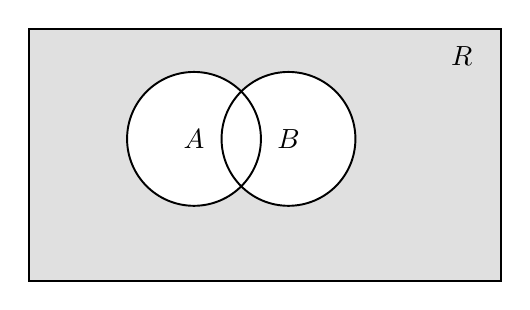
\begin{tikzpicture}[scale=1,line width=0.7pt]
\fill[black!12] (0,0) rectangle (6,3.2);
\fill[white] (2.1,1.8) circle (0.85);
\fill[white] (3.3,1.8) circle (0.85);
\draw (0,0) rectangle (6,3.2);
\draw (2.1,1.8) circle (0.85);
\draw (3.3,1.8) circle (0.85);
\node at (2.1,1.8) {$A$};
\node at (3.3,1.8) {$B$};
\node at (5.5,2.85) {$R$};
\end{tikzpicture}
\end{center}

（1）若集合 $C$ 表示图中阴影部分，用集合的运算式表示 $C$.

（2）求集合 $C$.

\ansspace*[12]

\ifanswer
\solbegin
\stepm{（1）}{由韦恩图得 $C=\overline{A\cup B}$.}
\stepm{（2）}{解 $\dfrac{x+1}{x-2}<-1$，则 $\dfrac{x+1}{x-2}+1<0$，即 $\dfrac{2x-1}{x-2}<0$，解得 $\dfrac12<x<2$，}
\step{故 $B=\left\{x\left|\dfrac12<x<2\right.\right\}$，所以 $A\cup B=\{x\mid-3\leqslant x<2\}$，}
\step{所以 $C=\overline{A\cup B}=\{x\mid x<-3\ \text{或}\ x\geqslant2\}$.}
\solend
\fi

\item 已知集合 $A=\{x\mid x^2-6x+8<0\}$，集合 $B=\{x\mid3m<x<1-m\}$.

（1）命题 $p:x\in A$，命题 $q:x\in B$，若 $p$ 是 $q$ 的充分条件，求实数 $m$ 的取值范围.

（2）若 $A\cap B=\varnothing$，求实数 $m$ 的取值范围.

\ansspace*[12]

\ifanswer
\solbegin
\stepm{（1）}{$x^2-6x+8<0\Rightarrow2<x<4\Rightarrow A=\{x\mid2<x<4\}$.}
\step{若 $p$ 是 $q$ 的充分条件，则 $A\subseteq B$，结合 $B$ 为非空集合，得 $\begin{cases}3m<1-m\\ 3m\leqslant2\\ 1-m\geqslant4\end{cases}$，}
\step{解得 $m\leqslant-3$，故 $m$ 的取值范围是 $(-\infty,-3]$；}
\stepm{（2）}{当 $B=\varnothing$ 时，$3m\geqslant1-m$，解得 $m\geqslant\dfrac14$，满足 $A\cap B=\varnothing$；}
\step{当 $B\neq\varnothing$ 时，$3m<1-m$ 即 $m<\dfrac14$，}
\step{要使交集为空，则 $1-m\leqslant2$ 或 $3m\geqslant4$，解得 $m\geqslant-1$，}
\step{结合 $m<\dfrac14$，得 $-1\leqslant m<\dfrac14$.}
\step{综上，$m\geqslant-1$，即 $m$ 的取值范围是 $[-1,+\infty)$.}
\solend
\fi

\item 设某企业每月生产电机 $x$ 台，根据企业月度报表知，每月总产值 $m$（万元）与总支出 $n$（万元）近似地满足下列关系：$m=\dfrac92x-\dfrac14$，$n=-\dfrac14x^2+5x+\dfrac74$，当 $m-n\geqslant0$ 时，称不亏损企业；当 $m-n<0$ 时，称亏损企业，且 $n-m$ 为亏损额.

（1）企业要成为不亏损企业，每月至少要生产多少台电机？

（2）当月总产值为多少时，企业亏损最严重，最大亏损额为多少？

\ansspace*[12]

\ifanswer
\solbegin
\stepm{（1）}{由题意得 $m-n\geqslant0$，即 $\dfrac92x-\dfrac14\geqslant-\dfrac14x^2+5x+\dfrac74$，}
\step{整理得 $x^2-2x-8\geqslant0$，解得 $x\geqslant4$ 或 $x\leqslant-2$（舍），}
\step{所以企业要成为不亏损企业，每月至少要生产 $4$ 台电机；}
\stepm{（2）}{由（1）得当 $0<x<4$ 时企业亏损，}
\step{亏损额 $n-m=\left(-\dfrac14x^2+5x+\dfrac74\right)-\left(\dfrac92x-\dfrac14\right)=-\dfrac14(x-1)^2+\dfrac94$，}
\step{所以当 $x=1$ 时，$n-m$ 取最大值 $\dfrac94$，}
\step{答：当月总产值为 $1$ 台时，企业亏损最严重，最大亏损额为 $\dfrac94$ 万元.}
\solend
\fi

\item 已知 $x_1$、$x_2$ 是一元二次方程 $4kx^2-4kx+k+1=0(k\neq0)$ 的两个实数根.

（1）是否存在实数 $k$，使 $x_1^2+x_2^2=\dfrac14$ 成立？若存在，求出 $k$ 的值，若不存在，请说明理由；

（2）是否存在整数 $k$，使 $\dfrac{x_1}{x_2}+\dfrac{x_2}{x_1}-2$ 的值为整数？若存在，求出 $k$ 的值，若不存在，请说明理由.

\ansspace*[14]

\ifanswer
\solbegin
\stepm{（1）}{因为 $x_1$、$x_2$ 是一元二次方程 $4kx^2-4kx+k+1=0(k\neq0)$ 的两个实数根，}
\step{所以 $\Delta=(-4k)^2-4\times4k(k+1)\geqslant0$，解得 $k\leqslant0$，}
\step{由韦达定理得 $\begin{cases}x_1+x_2=1\\ x_1x_2=\dfrac{k+1}{4k}\end{cases}$，}
\step{则 $x_1^2+x_2^2=(x_1+x_2)^2-2x_1x_2=\dfrac14$，}
\step{即 $1-2\times\dfrac{k+1}{4k}=\dfrac14$，解得 $k=2$，因为 $k\leqslant0$，所以不存在实数 $k$.}
\stepm{（2）}{$\dfrac{x_1}{x_2}+\dfrac{x_2}{x_1}-2=\dfrac{x_1^2+x_2^2}{x_1x_2}-2=\dfrac{(x_1+x_2)^2-2x_1x_2}{x_1x_2}-2=\dfrac{(x_1+x_2)^2}{x_1x_2}-4$}
\step{$=\dfrac{1}{\dfrac{k+1}{4k}}-4=\dfrac{4k}{k+1}-4=\dfrac{4k-4(k+1)}{k+1}=\dfrac{-4}{k+1}$，}
\step{由于 $\dfrac{x_1}{x_2}+\dfrac{x_2}{x_1}-2$ 的值为整数，即 $\dfrac{-4}{k+1}$ 的值为整数，}
\step{所以 $k+1$ 只能取 $\pm1$、$\pm2$、$\pm4$，}
\step{又 $k\leqslant0$，所以当 $k+1=\pm1$ 时，得出 $k=0$（舍）或 $k=-2$，}
\step{当 $k+1=\pm2$ 时，得出 $k=1$（舍）或 $k=-3$，}
\step{当 $k+1=\pm4$ 时，得出 $k=3$（舍）或 $k=-5$，}
\step{综上所述，若 $\dfrac{x_1}{x_2}+\dfrac{x_2}{x_1}-2$ 的值为整数，则 $k$ 的值为 $-2$ 或 $-3$ 或 $-5$.}
\solend
\fi

\item 已知集合 $A=\{a_1,a_2,\cdots,a_n\}(n\geqslant3)$，其中 $a_m\in\Z(m=1,2,\cdots,n)$. 若 $A$ 的子集 $T=\{a_i,a_j,a_k\}$ 满足 $2a_k=a_i+a_j$，则称 $T$ 具有性质 $P$. $A$ 的所有具有性质 $P$ 的子集 $T$ 的个数记为 $card_A(T)$.

（1）当 $A=\{4,-1,-2,1,-5\}$ 时，写出 $A$ 的所有具有性质 $P$ 的子集 $T$；

（2）当 $n=4$ 时，若 $a_1<a_2<a_3<a_4$，且 $card_A(T)=2$，证明：数对 $a_1$、$a_3$ 和 $a_2$、$a_4$ 中至少有一对中的两数奇偶性相同；

（3）当 $n=9$ 时，求 $card_A(T)$ 的最大值.

\ansspace*[14]

\ifanswer
\solbegin
\stepm{（1）}{集合 $A=\{4,-1,-2,1,-5\}$，元素按从小到大排列为 $-5$、$-2$、$-1$、$1$、$4$，}
\step{满足 $2a_k=a_i+a_j$ 的三元子集 $T$ 需满足其中一个元素是另外两个的平均数，}
\step{对于 $-5,-2,1$：$2\times(-2)=-4=-5+1$，满足条件，故 $T=\{-5,-2,1\}$，}
\step{对于 $-2,1,4$：$2\times1=2=-2+4$，满足条件，故 $T=\{-2,1,4\}$，}
\step{因此满足的子集有 $\{-5,-2,1\}$ 和 $\{-2,1,4\}$.}
\stepm{（2）}{假设数对 $(a_1,a_3)$ 和 $(a_2,a_4)$ 的两数奇偶性均不同，}
\step{即 $a_1$ 与 $a_3$ 一奇一偶，故 $a_1+a_3$ 为奇数，}
\step{$a_2$ 与 $a_4$ 一奇一偶，故 $a_2+a_4$ 为奇数，}
\step{集合 $A=\{a_1,a_2,a_3,a_4\}$ 的三元子集共 $\mathrm{C}_4^3=4$ 个：}
\step{$\{a_1,a_2,a_3\}$：若满足 $2a_2=a_1+a_3$，左边为偶数，右边为奇数，矛盾，故不满足；}
\step{$\{a_2,a_3,a_4\}$：若满足 $2a_3=a_2+a_4$，左边为偶数，右边为奇数，矛盾，故不满足；}
\step{$\{a_1,a_2,a_4\}$：需 $2a_2=a_1+a_4$；}
\step{$\{a_1,a_3,a_4\}$：需 $2a_3=a_1+a_4$.}
\step{若这两个子集都满足，则 $2a_2=2a_3\Rightarrow a_2=a_3$，与 $a_2<a_3$ 矛盾，}
\step{因此最多只有 $1$ 个子集满足条件，与 $card_A(T)=2$ 矛盾，故假设不成立，}
\step{即数对 $(a_1,a_3)$ 和 $(a_2,a_4)$ 中至少有一对的两数奇偶性相同.}
\stepm{（3）}{要最大化 $card_A(T)$，}
\step{集合 $A$ 应包含尽可能多的三元等差数列（即长度为 $3$ 的等差数列），}
\step{当 $A$ 为公差为 $1$ 的等差数列（如 $A=\{0,1,2,\cdots,8\}$）时，}
\step{三元等差数列的个数最多，}
\step{对于集合 $\{0,1,2,\cdots,8\}$，计算三元等差数列个数：}
\step{公差 $d=1$：$\{0,1,2\},\{1,2,3\},\cdots,\{6,7,8\}$，共 $7$ 个；}
\step{公差 $d=2$：$\{0,2,4\},\{1,3,5\},\cdots,\{4,6,8\}$，共 $5$ 个；}
\step{公差 $d=3$：$\{0,3,6\},\{1,4,7\},\{2,5,8\}$，共 $3$ 个；}
\step{公差 $d=4$：$\{0,4,8\}$，共 $1$ 个；}
\step{总个数为 $7+5+3+1=16$.}
\solend
\fi

\end{enumerate}

\end{document}
"
% 紧凑版：xelatex "\def\iscompact{1}% 高一89_宝山中学_10月月考.tex
%   —— 高一上数学“2026-2027 年宝山中学高一上 10 月月考”（讲评版）
% 试卷版：xelatex 高一89_宝山中学_10月月考.tex
% 答案版：xelatex "\def\isanswer{1}% 高一89_宝山中学_10月月考.tex
%   —— 高一上数学“2026-2027 年宝山中学高一上 10 月月考”（讲评版）
% 试卷版：xelatex 高一89_宝山中学_10月月考.tex
% 答案版：xelatex "\def\isanswer{1}\input{高一89_宝山中学_10月月考.tex}"
% 紧凑版：xelatex "\def\iscompact{1}\input{高一89_宝山中学_10月月考.tex}"
%
% 原始材料：微信公众号“魔都数学加油站”文章，连载“27学年高一89”；
% 原文标题“27学年高一89——2026-2027年上海市宝山中学高一上10月月考”；
% 原文链接：https://mp.weixin.qq.com/s/DZ-Q-hfS4UulNW_vGWrZXw。
% 正文为 10 张 PNG 页（`原图/高一89_宝山中学_10月月考/01..10.png`），
% 尺寸混排（第 6 页为 2560×3620，其余为 4762×6735），均按页序读取。
%
% 篇幅与题号：原卷自第 3 题起编号（第 1、2 题不在原文内）。填空题 3—12（10 题）、
% 选择题 13—16（4 题）、解答题 17—21（5 题），共 19 题。
%
% 讲评版：第 4 题只印【答案】（“$x\leqslant2$ 或 $y\leqslant2$”），本稿只给 \ans{}；
% 其余 18 题印【解析】，其中选择题答案在解析末句“故选 C／B／A／A”。
% 第 17 题题干带一幅韦恩图（全集 $R$、集合 $A$、$B$ 与阴影部分），三版都出。
%
% 副标题：原卷未印副标题。本稿按内容标作“集合与常用逻辑用语、不等式”。
%
% 原卷笔误/存疑（均照录未改，正文对应处另有 % 注）：
%   ① 第 8 题题干“$k\in R$”与第 12 题“$n\in N$”按原卷用斜体字母排，本稿沿用
%      $\R$、$\N$ 记号（见“排版差异”③），此处不再视为笔误；
%   ② 第 9 题解析“故 $a$ 的取值范围是 $a<-1$ 或 $\dfrac13<a<\dfrac12$”，未把
%      $a<-1$ 写成区间，与同题前两行的写法不统一，属原卷写法，照录；
%   ③ 第 20 题 (1) 由 $\Delta\geqslant0$ 得“$k\leqslant0$”，与题设 $k\neq0$ 合看
%      应为 $k<0$；原卷写 $k\leqslant0$ 并以之舍去 $k=2$，结论不变，照录。
%
% 与原卷的排版差异：
%   ① 原卷每题下直接印【答案】/【解析】，本稿按全稿惯例将答案与解析置于答案版；
%   ② 原卷未印副标题，本稿补出；填空横线统一排 \blankline[4.4em]；
%   ③ 原卷数集记号排斜体 $R$、$Z$、$N$，本稿按全稿惯例改用 $\R$、$\Z$、$\N$；
%   ④ 第 17—21 题的子问用行内“（1）（2）（3）”段，解析中的子问标号用 \stepm；
%   ⑤ 解答题按惯例加 \ansspace；选择题括号排 \mbox{（\quad）}；
%   ⑥ 第 17 题的韦恩图原卷排在题干右侧、文字绕排，本稿改排为题干后的居中图
%      （TikZ 重绘：原图该处有公众号粉色水印斜压，按原图布局重绘，标注一致）。
%
% 行数核对：逐题数 \step/\stepm 条数，合计 119 条（Q3：2；Q4：0；Q5：3；Q6：4；
% Q7：2；Q8：3；Q9：4；Q10：5；Q11：8；Q12：4；Q13：5；Q14：7；Q15：9；Q16：5；
% Q17：4；Q18：8；Q19：7；Q20：13；Q21：26）。第 4 题只印【答案】，不计入 \step 账。
% 原卷解析的换行按语意合并，未逐行强拆。
%
\documentclass[a4paper,11pt]{article}
\usepackage{common}

\begin{document}

\examtitlest[7]{2026--2027 年宝山中学高一上 10 月月考}{集合与常用逻辑用语、不等式}

\bigsec{一、填空题}

\begin{enumerate}
\setcounter{enumi}{2}

\item 满足 $\{1,2\}\subseteq A\subseteq\{1,2,3,4,5\}$ 的集合共 $A$ 有\blankline[4.4em]个.

\ifanswer
\solbegin
\step{由题意得 $A=\{1,2\}$ 与 $\{3,4,5\}$ 的非空子集的并集，}
\step{而 $\{3,4,5\}$ 的子集有 $2^3=8$ 个，所以满足条件的 $A$ 有 $8$ 个.}
\solend
\fi

\item 用反证法证明命题：“若 $x+y>4$，则 $x>2$ 且 $y>2$”时，第一步应该假设\blankline[4.4em].

\ifanswer
\ans{$x\leqslant2$ 或 $y\leqslant2$}
\fi

\item 已知等式 $2x^2+3x+5=a(2x+1)(x+1)+c$ 恒成立，则 $a-c$ 的值为\blankline[4.4em].

\ifanswer
\solbegin
\step{因为 $2x^2+3x+5=a(2x+1)(x+1)+c$ 恒成立，}
\step{所以 $2x^2+3x+5=2ax^2+3ax+a+c$ 恒成立，}
\step{则 $\begin{cases}2=2a\\ 3=3a\\ 5=a+c\end{cases}$，得 $a=1$，$c=4$，所以 $a-c=-3$.}
\solend
\fi

\item 不等式 $\lvert3x-1\rvert<x$ 的解集\blankline[4.4em].

\ifanswer
\solbegin
\step{当 $x\leqslant0$ 时，不等式的解集为 $\varnothing$，}
\step{当 $x>0$ 时，$\lvert3x-1\rvert<x$，即 $(3x-1)^2<x^2$，}
\step{整理得 $8x^2-6x+1<0$，$(2x-1)(4x-1)<0$，解得 $\dfrac14<x<\dfrac12$，满足 $x>0$.}
\step{故解集为 $\left(\dfrac14,\dfrac12\right)$.}
\solend
\fi

\item 比较两个代数式的大小关系：$x^2+2y^2$\blankline[3em]$2xy+2y-1$.

\ifanswer
\solbegin
\step{$x^2+2y^2-(2xy+2y-1)=x^2-2xy+y^2+y^2-2y+1$}
\step{$=(x-y)^2+(y-1)^2\geqslant0$，所以 $x^2+2y^2\geqslant2xy+2y-1$.}
\solend
\fi

\item $k\in\R$，关于 $x$ 的不等式 $x^2+\sqrt2kx+2>0$ 的解集为全体实数，则 $k$ 的取值范围是\blankline[4.4em].

\ifanswer
\solbegin
\step{因为关于 $x$ 的不等式 $x^2+\sqrt2kx+2>0$ 的解集为全体实数，}
\step{所以 $\Delta=(\sqrt2k)^2-4\times1\times2=2k^2-8<0$，解得 $-2<k<2$，}
\step{即实数 $k$ 的取值范围是 $(-2,2)$.}
\solend
\fi

\item 在平面直角坐标系内，点 $\left(2a-1,\dfrac{3a-1}{a+1}\right)$ 在第二象限，则 $a$ 的取值范围是\blankline[4.4em].

\ifanswer
\solbegin
\step{由题意得 $\begin{cases}2a-1<0\\[0.2em]\dfrac{3a-1}{a+1}>0\end{cases}$，}
\step{由 $2a-1<0$，解得 $a<\dfrac12$；}
\step{由 $\dfrac{3a-1}{a+1}>0$，解得 $a<-1$ 或 $a>\dfrac13$；}
\step{故 $a$ 的取值范围是 $a<-1$ 或 $\dfrac13<a<\dfrac12$.}
\solend
\fi

\item 设集合 $A=\{x\mid x^2+x-6=0\}$，集合 $B=\{x\mid mx+1=0\}$，且 $A\cup B=A$，则 $m$ 的值组成的集合是\blankline[4.4em].

\ifanswer
\solbegin
\step{由题意得 $A=\{x\mid x^2+x-6=0\}=\{-3,2\}$，}
\step{由 $A\cup B=A$，得 $B\subseteq A$，}
\step{当 $m=0$ 时，$B=\varnothing$，满足题意，}
\step{当 $m\neq0$ 时，$B=\left\{-\dfrac1m\right\}$，所以 $-\dfrac1m=2$ 或 $-\dfrac1m=-3$，所以 $m=-\dfrac12$ 或 $m=\dfrac13$，}
\step{综上所述，$m$ 的值组成的集合是 $\left\{0,-\dfrac12,\dfrac13\right\}$.}
\solend
\fi

\item 甲、乙两人解关于 $x$ 的不等式 $x^2+bx+c<0$，甲写错了 $b$，正确计算后得到的解为 $\{x\mid1<x<2\}$；乙写错了 $c$，正确计算后得到的解为 $\{x\mid-4<x<1\}$. 那么不等式 $\dfrac{bx+c}{x-2}<0$ 的解为\blankline[4.4em].

\ifanswer
\solbegin
\step{由 $x^2+bx+c<0$ 的解为 $\{x\mid1<x<2\}$，}
\step{则 $1$ 和 $2$ 是方程 $x^2+bx+c=0$ 的两个根，}
\step{甲写错了 $b$，但 $c$ 是正确的，所以 $c=1\times2=2$；}
\step{由 $x^2+bx+c<0$ 的解为 $\{x\mid-4<x<1\}$，}
\step{则 $-4$ 和 $1$ 是方程 $x^2+bx+c=0$ 的两个根，}
\step{乙写错了 $c$，但 $b$ 是正确的，所以 $-b=-4+1=-3$，即 $b=3$.}
\step{由 $\dfrac{bx+c}{x-2}<0$，得 $\dfrac{3x+2}{x-2}<0$，即 $(3x+2)(x-2)<0$，解得 $-\dfrac23<x<2$，}
\step{所以不等式 $\dfrac{bx+c}{x-2}<0$ 的解为 $\left\{x\left|-\dfrac23<x<2\right.\right\}$.}
\solend
\fi

\item 已知集合 $M$ 的元素均为正整数，定义集合 $M$ 的“变项和”为：将 $M$ 中每个元素 $m$ 都乘以 $(-1)^m$ 后再求和. 若集合 $A=\{n\mid1\leqslant n\leqslant10,n\in\N\}$，则集合 $A$ 的所有非空子集的“变项和”的总和为\blankline[4.4em].

\ifanswer
\solbegin
\step{$A$ 集合的所有非空子集中，每个元素出现的次数都是 $(2^{10}-1)-(2^9-1)=2^9$，}
\step{则集合 $A$ 的所有非空子集的“变项和”的总和}
\step{为 $1\times(-1)^1\times2^9+2\times(-1)^2\times2^9+\cdots+10\times(-1)^{10}\times2^9$}
\step{$=(-1+2-3+4-\cdots-9+10)\times2^9=5\times2^9=2560$.}
\solend
\fi

\end{enumerate}

\bigsec{二、选择题}

\begin{enumerate}
\setcounter{enumi}{12}

\item 下列命题中正确的是\mbox{（\quad）}

\keepwithprev
A. 若 $a>b$，则 $\dfrac1a<\dfrac1b$\qquad B. 若 $a>b$，则 $a^2>b^2$

C. 若 $a>\lvert b\rvert$，则 $a>b$\qquad D. 若 $a>b$，则 $ac^2>bc^2$

\ifanswer
\solbegin
\step{对于 $AB$ 选项，取 $a=1$，$b=-1$，$a>b$，$\dfrac1a>\dfrac1b$，$a^2=b^2$，}
\step{所以 $AB$ 选项错误；}
\step{对于 $C$ 选项，由 $a>\lvert b\rvert$，$\lvert b\rvert\geqslant b$，得 $a>b$，所以 $C$ 选项正确；}
\step{对于 $D$ 选项，取 $c=0$，则 $ac^2=0=bc^2$，所以 $D$ 选项错误.}
\step{故选 $C$.}
\solend
\fi

\item 下面关于集合的表示正确的个数是\mbox{（\quad）}

①$\{1,2,3\}=\{3,2,1\}$；\quad ②$\{(x,y)\mid x-y=1\}=\{y\mid y=x-1\}$；

③$\{x\mid x\geqslant2,x\in\N\}=\{y\mid y\geqslant2,y\in\Z\}$；\quad ④$\{x\mid x+2y=1\}\neq\left\{y\left|y=-\dfrac12x+\dfrac12\right.\right\}$.

\keepwithprev
A. $1$\qquad B. $2$\qquad C. $3$\qquad D. $4$

\ifanswer
\solbegin
\step{对于①，由元素的无序性得①正确；}
\step{对于②，$\{(x,y)\mid x-y=1\}$ 表示点集，$\{y\mid y=x-1\}$ 表示数集，故②错误；}
\step{对于③，$\{x\mid x\geqslant2,x\in\N\}$ 表示大于等于 $2$ 的整数，}
\step{$\{y\mid y\geqslant2,y\in\Z\}$ 也表示大于等于 $2$ 的整数，故③正确；}
\step{对于④，$\{x\mid x+2y=1\}=\R$，$\left\{y\left|y=-\dfrac12x+\dfrac12\right.\right\}=\R$，}
\step{所以 $\{x\mid x+2y=1\}=\left\{y\left|y=-\dfrac12x+\dfrac12\right.\right\}$，故④错误，}
\step{所以正确的个数是 $2$ 个. 故选 $B$.}
\solend
\fi

\item 已知命题 $P$：方程 $ax^2+bx+c=0$ 有两个不相等实根；命题 $Q$：不等式 $ax^2+bx+c>0$ 与 $ax^2+bx+c<0$ 均有解，则命题 $P$ 成立是命题 $Q$ 成立的\mbox{（\quad）}条件.

\keepwithprev
A. 充分非必要条件\qquad B. 必要非充分条件

C. 充要条件\qquad D. 既非充分又非必要条件

\ifanswer
\solbegin
\step{若 $P$ 成立，即方程 $ax^2+bx+c=0$ 有两个不相等实根，}
\step{此时 $\begin{cases}a\neq0\\ \Delta=b^2-4ac>0\end{cases}$；}
\step{若 $Q$ 成立，即不等式 $ax^2+bx+c>0$ 与 $ax^2+bx+c<0$ 均有解，有两种情况：}
\step{①不等式是一元二次不等式，}
\step{此时不等式所对应的二次函数的图像与 $x$ 轴有两个交点，}
\step{满足 $\begin{cases}a\neq0\\ \Delta=b^2-4ac>0\end{cases}$；}
\step{②不等式是一元一次不等式，此时 $\begin{cases}a=0\\ b\neq0\end{cases}$，}
\step{因此，由 $P$ 能推出 $Q$ 成立，但是由 $Q$ 不能推出 $P$ 成立，}
\step{即 $P$ 是 $Q$ 的充分非必要条件. 故选 $A$.}
\solend
\fi

\item 甲、乙同去加油站加油两次，两次汽油单价分别为 $x$、$y$ 元/升（$x\neq y$）. 甲每次加固定金额的油，乙每次加固定体积的油. 哪种方式更经济实惠呢？\mbox{（\quad）}

\keepwithprev
A. 加固定金额的方式\qquad B. 加固定体积的方式

C. 两种方案一样\qquad D. 要视具体价格而定

\ifanswer
\solbegin
\step{设两次加油的油价分别为 $x$、$y$（$x$、$y>0$，且 $x\neq y$），}
\step{乙每次加油的量为 $a$（$a>0$）；甲每次加油的钱数为 $b$（$b>0$），}
\step{则乙平均油价为 $\dfrac{ax+ay}{2a}=\dfrac{x+y}{2}$，甲平均油价为 $\dfrac{2b}{\dfrac bx+\dfrac by}=\dfrac2{\dfrac1x+\dfrac1y}=\dfrac{2xy}{x+y}$，}
\step{因为 $x\neq y$，所以 $\dfrac{x+y}{2}-\dfrac{2xy}{x+y}=\dfrac{(x-y)^2}{2(x+y)}>0$，所以 $\dfrac{x+y}{2}>\dfrac{2xy}{x+y}$，}
\step{即甲方案更经济. 故选 $A$.}
\solend
\fi

\end{enumerate}

\bigsec{三、解答题}

\begin{enumerate}
\setcounter{enumi}{16}

\item 已知全集 $U=\R$，集合 $A=\{x\mid-3\leqslant x\leqslant1\}$，$B=\left\{x\left|\dfrac{x+1}{x-2}<-1\right.\right\}$.

\begin{center}
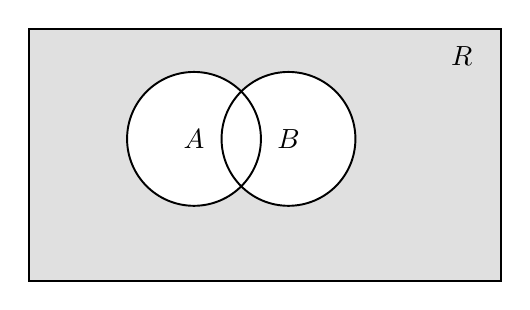
\begin{tikzpicture}[scale=1,line width=0.7pt]
\fill[black!12] (0,0) rectangle (6,3.2);
\fill[white] (2.1,1.8) circle (0.85);
\fill[white] (3.3,1.8) circle (0.85);
\draw (0,0) rectangle (6,3.2);
\draw (2.1,1.8) circle (0.85);
\draw (3.3,1.8) circle (0.85);
\node at (2.1,1.8) {$A$};
\node at (3.3,1.8) {$B$};
\node at (5.5,2.85) {$R$};
\end{tikzpicture}
\end{center}

（1）若集合 $C$ 表示图中阴影部分，用集合的运算式表示 $C$.

（2）求集合 $C$.

\ansspace*[12]

\ifanswer
\solbegin
\stepm{（1）}{由韦恩图得 $C=\overline{A\cup B}$.}
\stepm{（2）}{解 $\dfrac{x+1}{x-2}<-1$，则 $\dfrac{x+1}{x-2}+1<0$，即 $\dfrac{2x-1}{x-2}<0$，解得 $\dfrac12<x<2$，}
\step{故 $B=\left\{x\left|\dfrac12<x<2\right.\right\}$，所以 $A\cup B=\{x\mid-3\leqslant x<2\}$，}
\step{所以 $C=\overline{A\cup B}=\{x\mid x<-3\ \text{或}\ x\geqslant2\}$.}
\solend
\fi

\item 已知集合 $A=\{x\mid x^2-6x+8<0\}$，集合 $B=\{x\mid3m<x<1-m\}$.

（1）命题 $p:x\in A$，命题 $q:x\in B$，若 $p$ 是 $q$ 的充分条件，求实数 $m$ 的取值范围.

（2）若 $A\cap B=\varnothing$，求实数 $m$ 的取值范围.

\ansspace*[12]

\ifanswer
\solbegin
\stepm{（1）}{$x^2-6x+8<0\Rightarrow2<x<4\Rightarrow A=\{x\mid2<x<4\}$.}
\step{若 $p$ 是 $q$ 的充分条件，则 $A\subseteq B$，结合 $B$ 为非空集合，得 $\begin{cases}3m<1-m\\ 3m\leqslant2\\ 1-m\geqslant4\end{cases}$，}
\step{解得 $m\leqslant-3$，故 $m$ 的取值范围是 $(-\infty,-3]$；}
\stepm{（2）}{当 $B=\varnothing$ 时，$3m\geqslant1-m$，解得 $m\geqslant\dfrac14$，满足 $A\cap B=\varnothing$；}
\step{当 $B\neq\varnothing$ 时，$3m<1-m$ 即 $m<\dfrac14$，}
\step{要使交集为空，则 $1-m\leqslant2$ 或 $3m\geqslant4$，解得 $m\geqslant-1$，}
\step{结合 $m<\dfrac14$，得 $-1\leqslant m<\dfrac14$.}
\step{综上，$m\geqslant-1$，即 $m$ 的取值范围是 $[-1,+\infty)$.}
\solend
\fi

\item 设某企业每月生产电机 $x$ 台，根据企业月度报表知，每月总产值 $m$（万元）与总支出 $n$（万元）近似地满足下列关系：$m=\dfrac92x-\dfrac14$，$n=-\dfrac14x^2+5x+\dfrac74$，当 $m-n\geqslant0$ 时，称不亏损企业；当 $m-n<0$ 时，称亏损企业，且 $n-m$ 为亏损额.

（1）企业要成为不亏损企业，每月至少要生产多少台电机？

（2）当月总产值为多少时，企业亏损最严重，最大亏损额为多少？

\ansspace*[12]

\ifanswer
\solbegin
\stepm{（1）}{由题意得 $m-n\geqslant0$，即 $\dfrac92x-\dfrac14\geqslant-\dfrac14x^2+5x+\dfrac74$，}
\step{整理得 $x^2-2x-8\geqslant0$，解得 $x\geqslant4$ 或 $x\leqslant-2$（舍），}
\step{所以企业要成为不亏损企业，每月至少要生产 $4$ 台电机；}
\stepm{（2）}{由（1）得当 $0<x<4$ 时企业亏损，}
\step{亏损额 $n-m=\left(-\dfrac14x^2+5x+\dfrac74\right)-\left(\dfrac92x-\dfrac14\right)=-\dfrac14(x-1)^2+\dfrac94$，}
\step{所以当 $x=1$ 时，$n-m$ 取最大值 $\dfrac94$，}
\step{答：当月总产值为 $1$ 台时，企业亏损最严重，最大亏损额为 $\dfrac94$ 万元.}
\solend
\fi

\item 已知 $x_1$、$x_2$ 是一元二次方程 $4kx^2-4kx+k+1=0(k\neq0)$ 的两个实数根.

（1）是否存在实数 $k$，使 $x_1^2+x_2^2=\dfrac14$ 成立？若存在，求出 $k$ 的值，若不存在，请说明理由；

（2）是否存在整数 $k$，使 $\dfrac{x_1}{x_2}+\dfrac{x_2}{x_1}-2$ 的值为整数？若存在，求出 $k$ 的值，若不存在，请说明理由.

\ansspace*[14]

\ifanswer
\solbegin
\stepm{（1）}{因为 $x_1$、$x_2$ 是一元二次方程 $4kx^2-4kx+k+1=0(k\neq0)$ 的两个实数根，}
\step{所以 $\Delta=(-4k)^2-4\times4k(k+1)\geqslant0$，解得 $k\leqslant0$，}
\step{由韦达定理得 $\begin{cases}x_1+x_2=1\\ x_1x_2=\dfrac{k+1}{4k}\end{cases}$，}
\step{则 $x_1^2+x_2^2=(x_1+x_2)^2-2x_1x_2=\dfrac14$，}
\step{即 $1-2\times\dfrac{k+1}{4k}=\dfrac14$，解得 $k=2$，因为 $k\leqslant0$，所以不存在实数 $k$.}
\stepm{（2）}{$\dfrac{x_1}{x_2}+\dfrac{x_2}{x_1}-2=\dfrac{x_1^2+x_2^2}{x_1x_2}-2=\dfrac{(x_1+x_2)^2-2x_1x_2}{x_1x_2}-2=\dfrac{(x_1+x_2)^2}{x_1x_2}-4$}
\step{$=\dfrac{1}{\dfrac{k+1}{4k}}-4=\dfrac{4k}{k+1}-4=\dfrac{4k-4(k+1)}{k+1}=\dfrac{-4}{k+1}$，}
\step{由于 $\dfrac{x_1}{x_2}+\dfrac{x_2}{x_1}-2$ 的值为整数，即 $\dfrac{-4}{k+1}$ 的值为整数，}
\step{所以 $k+1$ 只能取 $\pm1$、$\pm2$、$\pm4$，}
\step{又 $k\leqslant0$，所以当 $k+1=\pm1$ 时，得出 $k=0$（舍）或 $k=-2$，}
\step{当 $k+1=\pm2$ 时，得出 $k=1$（舍）或 $k=-3$，}
\step{当 $k+1=\pm4$ 时，得出 $k=3$（舍）或 $k=-5$，}
\step{综上所述，若 $\dfrac{x_1}{x_2}+\dfrac{x_2}{x_1}-2$ 的值为整数，则 $k$ 的值为 $-2$ 或 $-3$ 或 $-5$.}
\solend
\fi

\item 已知集合 $A=\{a_1,a_2,\cdots,a_n\}(n\geqslant3)$，其中 $a_m\in\Z(m=1,2,\cdots,n)$. 若 $A$ 的子集 $T=\{a_i,a_j,a_k\}$ 满足 $2a_k=a_i+a_j$，则称 $T$ 具有性质 $P$. $A$ 的所有具有性质 $P$ 的子集 $T$ 的个数记为 $card_A(T)$.

（1）当 $A=\{4,-1,-2,1,-5\}$ 时，写出 $A$ 的所有具有性质 $P$ 的子集 $T$；

（2）当 $n=4$ 时，若 $a_1<a_2<a_3<a_4$，且 $card_A(T)=2$，证明：数对 $a_1$、$a_3$ 和 $a_2$、$a_4$ 中至少有一对中的两数奇偶性相同；

（3）当 $n=9$ 时，求 $card_A(T)$ 的最大值.

\ansspace*[14]

\ifanswer
\solbegin
\stepm{（1）}{集合 $A=\{4,-1,-2,1,-5\}$，元素按从小到大排列为 $-5$、$-2$、$-1$、$1$、$4$，}
\step{满足 $2a_k=a_i+a_j$ 的三元子集 $T$ 需满足其中一个元素是另外两个的平均数，}
\step{对于 $-5,-2,1$：$2\times(-2)=-4=-5+1$，满足条件，故 $T=\{-5,-2,1\}$，}
\step{对于 $-2,1,4$：$2\times1=2=-2+4$，满足条件，故 $T=\{-2,1,4\}$，}
\step{因此满足的子集有 $\{-5,-2,1\}$ 和 $\{-2,1,4\}$.}
\stepm{（2）}{假设数对 $(a_1,a_3)$ 和 $(a_2,a_4)$ 的两数奇偶性均不同，}
\step{即 $a_1$ 与 $a_3$ 一奇一偶，故 $a_1+a_3$ 为奇数，}
\step{$a_2$ 与 $a_4$ 一奇一偶，故 $a_2+a_4$ 为奇数，}
\step{集合 $A=\{a_1,a_2,a_3,a_4\}$ 的三元子集共 $\mathrm{C}_4^3=4$ 个：}
\step{$\{a_1,a_2,a_3\}$：若满足 $2a_2=a_1+a_3$，左边为偶数，右边为奇数，矛盾，故不满足；}
\step{$\{a_2,a_3,a_4\}$：若满足 $2a_3=a_2+a_4$，左边为偶数，右边为奇数，矛盾，故不满足；}
\step{$\{a_1,a_2,a_4\}$：需 $2a_2=a_1+a_4$；}
\step{$\{a_1,a_3,a_4\}$：需 $2a_3=a_1+a_4$.}
\step{若这两个子集都满足，则 $2a_2=2a_3\Rightarrow a_2=a_3$，与 $a_2<a_3$ 矛盾，}
\step{因此最多只有 $1$ 个子集满足条件，与 $card_A(T)=2$ 矛盾，故假设不成立，}
\step{即数对 $(a_1,a_3)$ 和 $(a_2,a_4)$ 中至少有一对的两数奇偶性相同.}
\stepm{（3）}{要最大化 $card_A(T)$，}
\step{集合 $A$ 应包含尽可能多的三元等差数列（即长度为 $3$ 的等差数列），}
\step{当 $A$ 为公差为 $1$ 的等差数列（如 $A=\{0,1,2,\cdots,8\}$）时，}
\step{三元等差数列的个数最多，}
\step{对于集合 $\{0,1,2,\cdots,8\}$，计算三元等差数列个数：}
\step{公差 $d=1$：$\{0,1,2\},\{1,2,3\},\cdots,\{6,7,8\}$，共 $7$ 个；}
\step{公差 $d=2$：$\{0,2,4\},\{1,3,5\},\cdots,\{4,6,8\}$，共 $5$ 个；}
\step{公差 $d=3$：$\{0,3,6\},\{1,4,7\},\{2,5,8\}$，共 $3$ 个；}
\step{公差 $d=4$：$\{0,4,8\}$，共 $1$ 个；}
\step{总个数为 $7+5+3+1=16$.}
\solend
\fi

\end{enumerate}

\end{document}
"
% 紧凑版：xelatex "\def\iscompact{1}% 高一89_宝山中学_10月月考.tex
%   —— 高一上数学“2026-2027 年宝山中学高一上 10 月月考”（讲评版）
% 试卷版：xelatex 高一89_宝山中学_10月月考.tex
% 答案版：xelatex "\def\isanswer{1}\input{高一89_宝山中学_10月月考.tex}"
% 紧凑版：xelatex "\def\iscompact{1}\input{高一89_宝山中学_10月月考.tex}"
%
% 原始材料：微信公众号“魔都数学加油站”文章，连载“27学年高一89”；
% 原文标题“27学年高一89——2026-2027年上海市宝山中学高一上10月月考”；
% 原文链接：https://mp.weixin.qq.com/s/DZ-Q-hfS4UulNW_vGWrZXw。
% 正文为 10 张 PNG 页（`原图/高一89_宝山中学_10月月考/01..10.png`），
% 尺寸混排（第 6 页为 2560×3620，其余为 4762×6735），均按页序读取。
%
% 篇幅与题号：原卷自第 3 题起编号（第 1、2 题不在原文内）。填空题 3—12（10 题）、
% 选择题 13—16（4 题）、解答题 17—21（5 题），共 19 题。
%
% 讲评版：第 4 题只印【答案】（“$x\leqslant2$ 或 $y\leqslant2$”），本稿只给 \ans{}；
% 其余 18 题印【解析】，其中选择题答案在解析末句“故选 C／B／A／A”。
% 第 17 题题干带一幅韦恩图（全集 $R$、集合 $A$、$B$ 与阴影部分），三版都出。
%
% 副标题：原卷未印副标题。本稿按内容标作“集合与常用逻辑用语、不等式”。
%
% 原卷笔误/存疑（均照录未改，正文对应处另有 % 注）：
%   ① 第 8 题题干“$k\in R$”与第 12 题“$n\in N$”按原卷用斜体字母排，本稿沿用
%      $\R$、$\N$ 记号（见“排版差异”③），此处不再视为笔误；
%   ② 第 9 题解析“故 $a$ 的取值范围是 $a<-1$ 或 $\dfrac13<a<\dfrac12$”，未把
%      $a<-1$ 写成区间，与同题前两行的写法不统一，属原卷写法，照录；
%   ③ 第 20 题 (1) 由 $\Delta\geqslant0$ 得“$k\leqslant0$”，与题设 $k\neq0$ 合看
%      应为 $k<0$；原卷写 $k\leqslant0$ 并以之舍去 $k=2$，结论不变，照录。
%
% 与原卷的排版差异：
%   ① 原卷每题下直接印【答案】/【解析】，本稿按全稿惯例将答案与解析置于答案版；
%   ② 原卷未印副标题，本稿补出；填空横线统一排 \blankline[4.4em]；
%   ③ 原卷数集记号排斜体 $R$、$Z$、$N$，本稿按全稿惯例改用 $\R$、$\Z$、$\N$；
%   ④ 第 17—21 题的子问用行内“（1）（2）（3）”段，解析中的子问标号用 \stepm；
%   ⑤ 解答题按惯例加 \ansspace；选择题括号排 \mbox{（\quad）}；
%   ⑥ 第 17 题的韦恩图原卷排在题干右侧、文字绕排，本稿改排为题干后的居中图
%      （TikZ 重绘：原图该处有公众号粉色水印斜压，按原图布局重绘，标注一致）。
%
% 行数核对：逐题数 \step/\stepm 条数，合计 119 条（Q3：2；Q4：0；Q5：3；Q6：4；
% Q7：2；Q8：3；Q9：4；Q10：5；Q11：8；Q12：4；Q13：5；Q14：7；Q15：9；Q16：5；
% Q17：4；Q18：8；Q19：7；Q20：13；Q21：26）。第 4 题只印【答案】，不计入 \step 账。
% 原卷解析的换行按语意合并，未逐行强拆。
%
\documentclass[a4paper,11pt]{article}
\usepackage{common}

\begin{document}

\examtitlest[7]{2026--2027 年宝山中学高一上 10 月月考}{集合与常用逻辑用语、不等式}

\bigsec{一、填空题}

\begin{enumerate}
\setcounter{enumi}{2}

\item 满足 $\{1,2\}\subseteq A\subseteq\{1,2,3,4,5\}$ 的集合共 $A$ 有\blankline[4.4em]个.

\ifanswer
\solbegin
\step{由题意得 $A=\{1,2\}$ 与 $\{3,4,5\}$ 的非空子集的并集，}
\step{而 $\{3,4,5\}$ 的子集有 $2^3=8$ 个，所以满足条件的 $A$ 有 $8$ 个.}
\solend
\fi

\item 用反证法证明命题：“若 $x+y>4$，则 $x>2$ 且 $y>2$”时，第一步应该假设\blankline[4.4em].

\ifanswer
\ans{$x\leqslant2$ 或 $y\leqslant2$}
\fi

\item 已知等式 $2x^2+3x+5=a(2x+1)(x+1)+c$ 恒成立，则 $a-c$ 的值为\blankline[4.4em].

\ifanswer
\solbegin
\step{因为 $2x^2+3x+5=a(2x+1)(x+1)+c$ 恒成立，}
\step{所以 $2x^2+3x+5=2ax^2+3ax+a+c$ 恒成立，}
\step{则 $\begin{cases}2=2a\\ 3=3a\\ 5=a+c\end{cases}$，得 $a=1$，$c=4$，所以 $a-c=-3$.}
\solend
\fi

\item 不等式 $\lvert3x-1\rvert<x$ 的解集\blankline[4.4em].

\ifanswer
\solbegin
\step{当 $x\leqslant0$ 时，不等式的解集为 $\varnothing$，}
\step{当 $x>0$ 时，$\lvert3x-1\rvert<x$，即 $(3x-1)^2<x^2$，}
\step{整理得 $8x^2-6x+1<0$，$(2x-1)(4x-1)<0$，解得 $\dfrac14<x<\dfrac12$，满足 $x>0$.}
\step{故解集为 $\left(\dfrac14,\dfrac12\right)$.}
\solend
\fi

\item 比较两个代数式的大小关系：$x^2+2y^2$\blankline[3em]$2xy+2y-1$.

\ifanswer
\solbegin
\step{$x^2+2y^2-(2xy+2y-1)=x^2-2xy+y^2+y^2-2y+1$}
\step{$=(x-y)^2+(y-1)^2\geqslant0$，所以 $x^2+2y^2\geqslant2xy+2y-1$.}
\solend
\fi

\item $k\in\R$，关于 $x$ 的不等式 $x^2+\sqrt2kx+2>0$ 的解集为全体实数，则 $k$ 的取值范围是\blankline[4.4em].

\ifanswer
\solbegin
\step{因为关于 $x$ 的不等式 $x^2+\sqrt2kx+2>0$ 的解集为全体实数，}
\step{所以 $\Delta=(\sqrt2k)^2-4\times1\times2=2k^2-8<0$，解得 $-2<k<2$，}
\step{即实数 $k$ 的取值范围是 $(-2,2)$.}
\solend
\fi

\item 在平面直角坐标系内，点 $\left(2a-1,\dfrac{3a-1}{a+1}\right)$ 在第二象限，则 $a$ 的取值范围是\blankline[4.4em].

\ifanswer
\solbegin
\step{由题意得 $\begin{cases}2a-1<0\\[0.2em]\dfrac{3a-1}{a+1}>0\end{cases}$，}
\step{由 $2a-1<0$，解得 $a<\dfrac12$；}
\step{由 $\dfrac{3a-1}{a+1}>0$，解得 $a<-1$ 或 $a>\dfrac13$；}
\step{故 $a$ 的取值范围是 $a<-1$ 或 $\dfrac13<a<\dfrac12$.}
\solend
\fi

\item 设集合 $A=\{x\mid x^2+x-6=0\}$，集合 $B=\{x\mid mx+1=0\}$，且 $A\cup B=A$，则 $m$ 的值组成的集合是\blankline[4.4em].

\ifanswer
\solbegin
\step{由题意得 $A=\{x\mid x^2+x-6=0\}=\{-3,2\}$，}
\step{由 $A\cup B=A$，得 $B\subseteq A$，}
\step{当 $m=0$ 时，$B=\varnothing$，满足题意，}
\step{当 $m\neq0$ 时，$B=\left\{-\dfrac1m\right\}$，所以 $-\dfrac1m=2$ 或 $-\dfrac1m=-3$，所以 $m=-\dfrac12$ 或 $m=\dfrac13$，}
\step{综上所述，$m$ 的值组成的集合是 $\left\{0,-\dfrac12,\dfrac13\right\}$.}
\solend
\fi

\item 甲、乙两人解关于 $x$ 的不等式 $x^2+bx+c<0$，甲写错了 $b$，正确计算后得到的解为 $\{x\mid1<x<2\}$；乙写错了 $c$，正确计算后得到的解为 $\{x\mid-4<x<1\}$. 那么不等式 $\dfrac{bx+c}{x-2}<0$ 的解为\blankline[4.4em].

\ifanswer
\solbegin
\step{由 $x^2+bx+c<0$ 的解为 $\{x\mid1<x<2\}$，}
\step{则 $1$ 和 $2$ 是方程 $x^2+bx+c=0$ 的两个根，}
\step{甲写错了 $b$，但 $c$ 是正确的，所以 $c=1\times2=2$；}
\step{由 $x^2+bx+c<0$ 的解为 $\{x\mid-4<x<1\}$，}
\step{则 $-4$ 和 $1$ 是方程 $x^2+bx+c=0$ 的两个根，}
\step{乙写错了 $c$，但 $b$ 是正确的，所以 $-b=-4+1=-3$，即 $b=3$.}
\step{由 $\dfrac{bx+c}{x-2}<0$，得 $\dfrac{3x+2}{x-2}<0$，即 $(3x+2)(x-2)<0$，解得 $-\dfrac23<x<2$，}
\step{所以不等式 $\dfrac{bx+c}{x-2}<0$ 的解为 $\left\{x\left|-\dfrac23<x<2\right.\right\}$.}
\solend
\fi

\item 已知集合 $M$ 的元素均为正整数，定义集合 $M$ 的“变项和”为：将 $M$ 中每个元素 $m$ 都乘以 $(-1)^m$ 后再求和. 若集合 $A=\{n\mid1\leqslant n\leqslant10,n\in\N\}$，则集合 $A$ 的所有非空子集的“变项和”的总和为\blankline[4.4em].

\ifanswer
\solbegin
\step{$A$ 集合的所有非空子集中，每个元素出现的次数都是 $(2^{10}-1)-(2^9-1)=2^9$，}
\step{则集合 $A$ 的所有非空子集的“变项和”的总和}
\step{为 $1\times(-1)^1\times2^9+2\times(-1)^2\times2^9+\cdots+10\times(-1)^{10}\times2^9$}
\step{$=(-1+2-3+4-\cdots-9+10)\times2^9=5\times2^9=2560$.}
\solend
\fi

\end{enumerate}

\bigsec{二、选择题}

\begin{enumerate}
\setcounter{enumi}{12}

\item 下列命题中正确的是\mbox{（\quad）}

\keepwithprev
A. 若 $a>b$，则 $\dfrac1a<\dfrac1b$\qquad B. 若 $a>b$，则 $a^2>b^2$

C. 若 $a>\lvert b\rvert$，则 $a>b$\qquad D. 若 $a>b$，则 $ac^2>bc^2$

\ifanswer
\solbegin
\step{对于 $AB$ 选项，取 $a=1$，$b=-1$，$a>b$，$\dfrac1a>\dfrac1b$，$a^2=b^2$，}
\step{所以 $AB$ 选项错误；}
\step{对于 $C$ 选项，由 $a>\lvert b\rvert$，$\lvert b\rvert\geqslant b$，得 $a>b$，所以 $C$ 选项正确；}
\step{对于 $D$ 选项，取 $c=0$，则 $ac^2=0=bc^2$，所以 $D$ 选项错误.}
\step{故选 $C$.}
\solend
\fi

\item 下面关于集合的表示正确的个数是\mbox{（\quad）}

①$\{1,2,3\}=\{3,2,1\}$；\quad ②$\{(x,y)\mid x-y=1\}=\{y\mid y=x-1\}$；

③$\{x\mid x\geqslant2,x\in\N\}=\{y\mid y\geqslant2,y\in\Z\}$；\quad ④$\{x\mid x+2y=1\}\neq\left\{y\left|y=-\dfrac12x+\dfrac12\right.\right\}$.

\keepwithprev
A. $1$\qquad B. $2$\qquad C. $3$\qquad D. $4$

\ifanswer
\solbegin
\step{对于①，由元素的无序性得①正确；}
\step{对于②，$\{(x,y)\mid x-y=1\}$ 表示点集，$\{y\mid y=x-1\}$ 表示数集，故②错误；}
\step{对于③，$\{x\mid x\geqslant2,x\in\N\}$ 表示大于等于 $2$ 的整数，}
\step{$\{y\mid y\geqslant2,y\in\Z\}$ 也表示大于等于 $2$ 的整数，故③正确；}
\step{对于④，$\{x\mid x+2y=1\}=\R$，$\left\{y\left|y=-\dfrac12x+\dfrac12\right.\right\}=\R$，}
\step{所以 $\{x\mid x+2y=1\}=\left\{y\left|y=-\dfrac12x+\dfrac12\right.\right\}$，故④错误，}
\step{所以正确的个数是 $2$ 个. 故选 $B$.}
\solend
\fi

\item 已知命题 $P$：方程 $ax^2+bx+c=0$ 有两个不相等实根；命题 $Q$：不等式 $ax^2+bx+c>0$ 与 $ax^2+bx+c<0$ 均有解，则命题 $P$ 成立是命题 $Q$ 成立的\mbox{（\quad）}条件.

\keepwithprev
A. 充分非必要条件\qquad B. 必要非充分条件

C. 充要条件\qquad D. 既非充分又非必要条件

\ifanswer
\solbegin
\step{若 $P$ 成立，即方程 $ax^2+bx+c=0$ 有两个不相等实根，}
\step{此时 $\begin{cases}a\neq0\\ \Delta=b^2-4ac>0\end{cases}$；}
\step{若 $Q$ 成立，即不等式 $ax^2+bx+c>0$ 与 $ax^2+bx+c<0$ 均有解，有两种情况：}
\step{①不等式是一元二次不等式，}
\step{此时不等式所对应的二次函数的图像与 $x$ 轴有两个交点，}
\step{满足 $\begin{cases}a\neq0\\ \Delta=b^2-4ac>0\end{cases}$；}
\step{②不等式是一元一次不等式，此时 $\begin{cases}a=0\\ b\neq0\end{cases}$，}
\step{因此，由 $P$ 能推出 $Q$ 成立，但是由 $Q$ 不能推出 $P$ 成立，}
\step{即 $P$ 是 $Q$ 的充分非必要条件. 故选 $A$.}
\solend
\fi

\item 甲、乙同去加油站加油两次，两次汽油单价分别为 $x$、$y$ 元/升（$x\neq y$）. 甲每次加固定金额的油，乙每次加固定体积的油. 哪种方式更经济实惠呢？\mbox{（\quad）}

\keepwithprev
A. 加固定金额的方式\qquad B. 加固定体积的方式

C. 两种方案一样\qquad D. 要视具体价格而定

\ifanswer
\solbegin
\step{设两次加油的油价分别为 $x$、$y$（$x$、$y>0$，且 $x\neq y$），}
\step{乙每次加油的量为 $a$（$a>0$）；甲每次加油的钱数为 $b$（$b>0$），}
\step{则乙平均油价为 $\dfrac{ax+ay}{2a}=\dfrac{x+y}{2}$，甲平均油价为 $\dfrac{2b}{\dfrac bx+\dfrac by}=\dfrac2{\dfrac1x+\dfrac1y}=\dfrac{2xy}{x+y}$，}
\step{因为 $x\neq y$，所以 $\dfrac{x+y}{2}-\dfrac{2xy}{x+y}=\dfrac{(x-y)^2}{2(x+y)}>0$，所以 $\dfrac{x+y}{2}>\dfrac{2xy}{x+y}$，}
\step{即甲方案更经济. 故选 $A$.}
\solend
\fi

\end{enumerate}

\bigsec{三、解答题}

\begin{enumerate}
\setcounter{enumi}{16}

\item 已知全集 $U=\R$，集合 $A=\{x\mid-3\leqslant x\leqslant1\}$，$B=\left\{x\left|\dfrac{x+1}{x-2}<-1\right.\right\}$.

\begin{center}
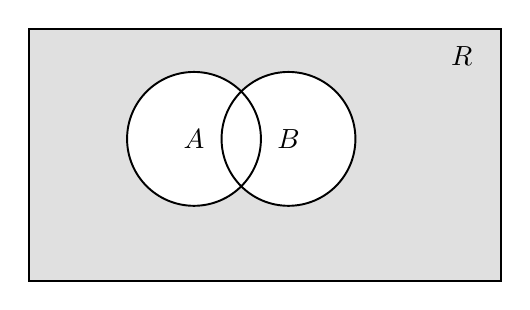
\begin{tikzpicture}[scale=1,line width=0.7pt]
\fill[black!12] (0,0) rectangle (6,3.2);
\fill[white] (2.1,1.8) circle (0.85);
\fill[white] (3.3,1.8) circle (0.85);
\draw (0,0) rectangle (6,3.2);
\draw (2.1,1.8) circle (0.85);
\draw (3.3,1.8) circle (0.85);
\node at (2.1,1.8) {$A$};
\node at (3.3,1.8) {$B$};
\node at (5.5,2.85) {$R$};
\end{tikzpicture}
\end{center}

（1）若集合 $C$ 表示图中阴影部分，用集合的运算式表示 $C$.

（2）求集合 $C$.

\ansspace*[12]

\ifanswer
\solbegin
\stepm{（1）}{由韦恩图得 $C=\overline{A\cup B}$.}
\stepm{（2）}{解 $\dfrac{x+1}{x-2}<-1$，则 $\dfrac{x+1}{x-2}+1<0$，即 $\dfrac{2x-1}{x-2}<0$，解得 $\dfrac12<x<2$，}
\step{故 $B=\left\{x\left|\dfrac12<x<2\right.\right\}$，所以 $A\cup B=\{x\mid-3\leqslant x<2\}$，}
\step{所以 $C=\overline{A\cup B}=\{x\mid x<-3\ \text{或}\ x\geqslant2\}$.}
\solend
\fi

\item 已知集合 $A=\{x\mid x^2-6x+8<0\}$，集合 $B=\{x\mid3m<x<1-m\}$.

（1）命题 $p:x\in A$，命题 $q:x\in B$，若 $p$ 是 $q$ 的充分条件，求实数 $m$ 的取值范围.

（2）若 $A\cap B=\varnothing$，求实数 $m$ 的取值范围.

\ansspace*[12]

\ifanswer
\solbegin
\stepm{（1）}{$x^2-6x+8<0\Rightarrow2<x<4\Rightarrow A=\{x\mid2<x<4\}$.}
\step{若 $p$ 是 $q$ 的充分条件，则 $A\subseteq B$，结合 $B$ 为非空集合，得 $\begin{cases}3m<1-m\\ 3m\leqslant2\\ 1-m\geqslant4\end{cases}$，}
\step{解得 $m\leqslant-3$，故 $m$ 的取值范围是 $(-\infty,-3]$；}
\stepm{（2）}{当 $B=\varnothing$ 时，$3m\geqslant1-m$，解得 $m\geqslant\dfrac14$，满足 $A\cap B=\varnothing$；}
\step{当 $B\neq\varnothing$ 时，$3m<1-m$ 即 $m<\dfrac14$，}
\step{要使交集为空，则 $1-m\leqslant2$ 或 $3m\geqslant4$，解得 $m\geqslant-1$，}
\step{结合 $m<\dfrac14$，得 $-1\leqslant m<\dfrac14$.}
\step{综上，$m\geqslant-1$，即 $m$ 的取值范围是 $[-1,+\infty)$.}
\solend
\fi

\item 设某企业每月生产电机 $x$ 台，根据企业月度报表知，每月总产值 $m$（万元）与总支出 $n$（万元）近似地满足下列关系：$m=\dfrac92x-\dfrac14$，$n=-\dfrac14x^2+5x+\dfrac74$，当 $m-n\geqslant0$ 时，称不亏损企业；当 $m-n<0$ 时，称亏损企业，且 $n-m$ 为亏损额.

（1）企业要成为不亏损企业，每月至少要生产多少台电机？

（2）当月总产值为多少时，企业亏损最严重，最大亏损额为多少？

\ansspace*[12]

\ifanswer
\solbegin
\stepm{（1）}{由题意得 $m-n\geqslant0$，即 $\dfrac92x-\dfrac14\geqslant-\dfrac14x^2+5x+\dfrac74$，}
\step{整理得 $x^2-2x-8\geqslant0$，解得 $x\geqslant4$ 或 $x\leqslant-2$（舍），}
\step{所以企业要成为不亏损企业，每月至少要生产 $4$ 台电机；}
\stepm{（2）}{由（1）得当 $0<x<4$ 时企业亏损，}
\step{亏损额 $n-m=\left(-\dfrac14x^2+5x+\dfrac74\right)-\left(\dfrac92x-\dfrac14\right)=-\dfrac14(x-1)^2+\dfrac94$，}
\step{所以当 $x=1$ 时，$n-m$ 取最大值 $\dfrac94$，}
\step{答：当月总产值为 $1$ 台时，企业亏损最严重，最大亏损额为 $\dfrac94$ 万元.}
\solend
\fi

\item 已知 $x_1$、$x_2$ 是一元二次方程 $4kx^2-4kx+k+1=0(k\neq0)$ 的两个实数根.

（1）是否存在实数 $k$，使 $x_1^2+x_2^2=\dfrac14$ 成立？若存在，求出 $k$ 的值，若不存在，请说明理由；

（2）是否存在整数 $k$，使 $\dfrac{x_1}{x_2}+\dfrac{x_2}{x_1}-2$ 的值为整数？若存在，求出 $k$ 的值，若不存在，请说明理由.

\ansspace*[14]

\ifanswer
\solbegin
\stepm{（1）}{因为 $x_1$、$x_2$ 是一元二次方程 $4kx^2-4kx+k+1=0(k\neq0)$ 的两个实数根，}
\step{所以 $\Delta=(-4k)^2-4\times4k(k+1)\geqslant0$，解得 $k\leqslant0$，}
\step{由韦达定理得 $\begin{cases}x_1+x_2=1\\ x_1x_2=\dfrac{k+1}{4k}\end{cases}$，}
\step{则 $x_1^2+x_2^2=(x_1+x_2)^2-2x_1x_2=\dfrac14$，}
\step{即 $1-2\times\dfrac{k+1}{4k}=\dfrac14$，解得 $k=2$，因为 $k\leqslant0$，所以不存在实数 $k$.}
\stepm{（2）}{$\dfrac{x_1}{x_2}+\dfrac{x_2}{x_1}-2=\dfrac{x_1^2+x_2^2}{x_1x_2}-2=\dfrac{(x_1+x_2)^2-2x_1x_2}{x_1x_2}-2=\dfrac{(x_1+x_2)^2}{x_1x_2}-4$}
\step{$=\dfrac{1}{\dfrac{k+1}{4k}}-4=\dfrac{4k}{k+1}-4=\dfrac{4k-4(k+1)}{k+1}=\dfrac{-4}{k+1}$，}
\step{由于 $\dfrac{x_1}{x_2}+\dfrac{x_2}{x_1}-2$ 的值为整数，即 $\dfrac{-4}{k+1}$ 的值为整数，}
\step{所以 $k+1$ 只能取 $\pm1$、$\pm2$、$\pm4$，}
\step{又 $k\leqslant0$，所以当 $k+1=\pm1$ 时，得出 $k=0$（舍）或 $k=-2$，}
\step{当 $k+1=\pm2$ 时，得出 $k=1$（舍）或 $k=-3$，}
\step{当 $k+1=\pm4$ 时，得出 $k=3$（舍）或 $k=-5$，}
\step{综上所述，若 $\dfrac{x_1}{x_2}+\dfrac{x_2}{x_1}-2$ 的值为整数，则 $k$ 的值为 $-2$ 或 $-3$ 或 $-5$.}
\solend
\fi

\item 已知集合 $A=\{a_1,a_2,\cdots,a_n\}(n\geqslant3)$，其中 $a_m\in\Z(m=1,2,\cdots,n)$. 若 $A$ 的子集 $T=\{a_i,a_j,a_k\}$ 满足 $2a_k=a_i+a_j$，则称 $T$ 具有性质 $P$. $A$ 的所有具有性质 $P$ 的子集 $T$ 的个数记为 $card_A(T)$.

（1）当 $A=\{4,-1,-2,1,-5\}$ 时，写出 $A$ 的所有具有性质 $P$ 的子集 $T$；

（2）当 $n=4$ 时，若 $a_1<a_2<a_3<a_4$，且 $card_A(T)=2$，证明：数对 $a_1$、$a_3$ 和 $a_2$、$a_4$ 中至少有一对中的两数奇偶性相同；

（3）当 $n=9$ 时，求 $card_A(T)$ 的最大值.

\ansspace*[14]

\ifanswer
\solbegin
\stepm{（1）}{集合 $A=\{4,-1,-2,1,-5\}$，元素按从小到大排列为 $-5$、$-2$、$-1$、$1$、$4$，}
\step{满足 $2a_k=a_i+a_j$ 的三元子集 $T$ 需满足其中一个元素是另外两个的平均数，}
\step{对于 $-5,-2,1$：$2\times(-2)=-4=-5+1$，满足条件，故 $T=\{-5,-2,1\}$，}
\step{对于 $-2,1,4$：$2\times1=2=-2+4$，满足条件，故 $T=\{-2,1,4\}$，}
\step{因此满足的子集有 $\{-5,-2,1\}$ 和 $\{-2,1,4\}$.}
\stepm{（2）}{假设数对 $(a_1,a_3)$ 和 $(a_2,a_4)$ 的两数奇偶性均不同，}
\step{即 $a_1$ 与 $a_3$ 一奇一偶，故 $a_1+a_3$ 为奇数，}
\step{$a_2$ 与 $a_4$ 一奇一偶，故 $a_2+a_4$ 为奇数，}
\step{集合 $A=\{a_1,a_2,a_3,a_4\}$ 的三元子集共 $\mathrm{C}_4^3=4$ 个：}
\step{$\{a_1,a_2,a_3\}$：若满足 $2a_2=a_1+a_3$，左边为偶数，右边为奇数，矛盾，故不满足；}
\step{$\{a_2,a_3,a_4\}$：若满足 $2a_3=a_2+a_4$，左边为偶数，右边为奇数，矛盾，故不满足；}
\step{$\{a_1,a_2,a_4\}$：需 $2a_2=a_1+a_4$；}
\step{$\{a_1,a_3,a_4\}$：需 $2a_3=a_1+a_4$.}
\step{若这两个子集都满足，则 $2a_2=2a_3\Rightarrow a_2=a_3$，与 $a_2<a_3$ 矛盾，}
\step{因此最多只有 $1$ 个子集满足条件，与 $card_A(T)=2$ 矛盾，故假设不成立，}
\step{即数对 $(a_1,a_3)$ 和 $(a_2,a_4)$ 中至少有一对的两数奇偶性相同.}
\stepm{（3）}{要最大化 $card_A(T)$，}
\step{集合 $A$ 应包含尽可能多的三元等差数列（即长度为 $3$ 的等差数列），}
\step{当 $A$ 为公差为 $1$ 的等差数列（如 $A=\{0,1,2,\cdots,8\}$）时，}
\step{三元等差数列的个数最多，}
\step{对于集合 $\{0,1,2,\cdots,8\}$，计算三元等差数列个数：}
\step{公差 $d=1$：$\{0,1,2\},\{1,2,3\},\cdots,\{6,7,8\}$，共 $7$ 个；}
\step{公差 $d=2$：$\{0,2,4\},\{1,3,5\},\cdots,\{4,6,8\}$，共 $5$ 个；}
\step{公差 $d=3$：$\{0,3,6\},\{1,4,7\},\{2,5,8\}$，共 $3$ 个；}
\step{公差 $d=4$：$\{0,4,8\}$，共 $1$ 个；}
\step{总个数为 $7+5+3+1=16$.}
\solend
\fi

\end{enumerate}

\end{document}
"
%
% 原始材料：微信公众号“魔都数学加油站”文章，连载“27学年高一89”；
% 原文标题“27学年高一89——2026-2027年上海市宝山中学高一上10月月考”；
% 原文链接：https://mp.weixin.qq.com/s/DZ-Q-hfS4UulNW_vGWrZXw。
% 正文为 10 张 PNG 页（`原图/高一89_宝山中学_10月月考/01..10.png`），
% 尺寸混排（第 6 页为 2560×3620，其余为 4762×6735），均按页序读取。
%
% 篇幅与题号：原卷自第 3 题起编号（第 1、2 题不在原文内）。填空题 3—12（10 题）、
% 选择题 13—16（4 题）、解答题 17—21（5 题），共 19 题。
%
% 讲评版：第 4 题只印【答案】（“$x\leqslant2$ 或 $y\leqslant2$”），本稿只给 \ans{}；
% 其余 18 题印【解析】，其中选择题答案在解析末句“故选 C／B／A／A”。
% 第 17 题题干带一幅韦恩图（全集 $R$、集合 $A$、$B$ 与阴影部分），三版都出。
%
% 副标题：原卷未印副标题。本稿按内容标作“集合与常用逻辑用语、不等式”。
%
% 原卷笔误/存疑（均照录未改，正文对应处另有 % 注）：
%   ① 第 8 题题干“$k\in R$”与第 12 题“$n\in N$”按原卷用斜体字母排，本稿沿用
%      $\R$、$\N$ 记号（见“排版差异”③），此处不再视为笔误；
%   ② 第 9 题解析“故 $a$ 的取值范围是 $a<-1$ 或 $\dfrac13<a<\dfrac12$”，未把
%      $a<-1$ 写成区间，与同题前两行的写法不统一，属原卷写法，照录；
%   ③ 第 20 题 (1) 由 $\Delta\geqslant0$ 得“$k\leqslant0$”，与题设 $k\neq0$ 合看
%      应为 $k<0$；原卷写 $k\leqslant0$ 并以之舍去 $k=2$，结论不变，照录。
%
% 与原卷的排版差异：
%   ① 原卷每题下直接印【答案】/【解析】，本稿按全稿惯例将答案与解析置于答案版；
%   ② 原卷未印副标题，本稿补出；填空横线统一排 \blankline[4.4em]；
%   ③ 原卷数集记号排斜体 $R$、$Z$、$N$，本稿按全稿惯例改用 $\R$、$\Z$、$\N$；
%   ④ 第 17—21 题的子问用行内“（1）（2）（3）”段，解析中的子问标号用 \stepm；
%   ⑤ 解答题按惯例加 \ansspace；选择题括号排 \mbox{（\quad）}；
%   ⑥ 第 17 题的韦恩图原卷排在题干右侧、文字绕排，本稿改排为题干后的居中图
%      （TikZ 重绘：原图该处有公众号粉色水印斜压，按原图布局重绘，标注一致）。
%
% 行数核对：逐题数 \step/\stepm 条数，合计 119 条（Q3：2；Q4：0；Q5：3；Q6：4；
% Q7：2；Q8：3；Q9：4；Q10：5；Q11：8；Q12：4；Q13：5；Q14：7；Q15：9；Q16：5；
% Q17：4；Q18：8；Q19：7；Q20：13；Q21：26）。第 4 题只印【答案】，不计入 \step 账。
% 原卷解析的换行按语意合并，未逐行强拆。
%
\documentclass[a4paper,11pt]{article}
\usepackage{common}

\begin{document}

\examtitlest[7]{2026--2027 年宝山中学高一上 10 月月考}{集合与常用逻辑用语、不等式}

\bigsec{一、填空题}

\begin{enumerate}
\setcounter{enumi}{2}

\item 满足 $\{1,2\}\subseteq A\subseteq\{1,2,3,4,5\}$ 的集合共 $A$ 有\blankline[4.4em]个.

\ifanswer
\solbegin
\step{由题意得 $A=\{1,2\}$ 与 $\{3,4,5\}$ 的非空子集的并集，}
\step{而 $\{3,4,5\}$ 的子集有 $2^3=8$ 个，所以满足条件的 $A$ 有 $8$ 个.}
\solend
\fi

\item 用反证法证明命题：“若 $x+y>4$，则 $x>2$ 且 $y>2$”时，第一步应该假设\blankline[4.4em].

\ifanswer
\ans{$x\leqslant2$ 或 $y\leqslant2$}
\fi

\item 已知等式 $2x^2+3x+5=a(2x+1)(x+1)+c$ 恒成立，则 $a-c$ 的值为\blankline[4.4em].

\ifanswer
\solbegin
\step{因为 $2x^2+3x+5=a(2x+1)(x+1)+c$ 恒成立，}
\step{所以 $2x^2+3x+5=2ax^2+3ax+a+c$ 恒成立，}
\step{则 $\begin{cases}2=2a\\ 3=3a\\ 5=a+c\end{cases}$，得 $a=1$，$c=4$，所以 $a-c=-3$.}
\solend
\fi

\item 不等式 $\lvert3x-1\rvert<x$ 的解集\blankline[4.4em].

\ifanswer
\solbegin
\step{当 $x\leqslant0$ 时，不等式的解集为 $\varnothing$，}
\step{当 $x>0$ 时，$\lvert3x-1\rvert<x$，即 $(3x-1)^2<x^2$，}
\step{整理得 $8x^2-6x+1<0$，$(2x-1)(4x-1)<0$，解得 $\dfrac14<x<\dfrac12$，满足 $x>0$.}
\step{故解集为 $\left(\dfrac14,\dfrac12\right)$.}
\solend
\fi

\item 比较两个代数式的大小关系：$x^2+2y^2$\blankline[3em]$2xy+2y-1$.

\ifanswer
\solbegin
\step{$x^2+2y^2-(2xy+2y-1)=x^2-2xy+y^2+y^2-2y+1$}
\step{$=(x-y)^2+(y-1)^2\geqslant0$，所以 $x^2+2y^2\geqslant2xy+2y-1$.}
\solend
\fi

\item $k\in\R$，关于 $x$ 的不等式 $x^2+\sqrt2kx+2>0$ 的解集为全体实数，则 $k$ 的取值范围是\blankline[4.4em].

\ifanswer
\solbegin
\step{因为关于 $x$ 的不等式 $x^2+\sqrt2kx+2>0$ 的解集为全体实数，}
\step{所以 $\Delta=(\sqrt2k)^2-4\times1\times2=2k^2-8<0$，解得 $-2<k<2$，}
\step{即实数 $k$ 的取值范围是 $(-2,2)$.}
\solend
\fi

\item 在平面直角坐标系内，点 $\left(2a-1,\dfrac{3a-1}{a+1}\right)$ 在第二象限，则 $a$ 的取值范围是\blankline[4.4em].

\ifanswer
\solbegin
\step{由题意得 $\begin{cases}2a-1<0\\[0.2em]\dfrac{3a-1}{a+1}>0\end{cases}$，}
\step{由 $2a-1<0$，解得 $a<\dfrac12$；}
\step{由 $\dfrac{3a-1}{a+1}>0$，解得 $a<-1$ 或 $a>\dfrac13$；}
\step{故 $a$ 的取值范围是 $a<-1$ 或 $\dfrac13<a<\dfrac12$.}
\solend
\fi

\item 设集合 $A=\{x\mid x^2+x-6=0\}$，集合 $B=\{x\mid mx+1=0\}$，且 $A\cup B=A$，则 $m$ 的值组成的集合是\blankline[4.4em].

\ifanswer
\solbegin
\step{由题意得 $A=\{x\mid x^2+x-6=0\}=\{-3,2\}$，}
\step{由 $A\cup B=A$，得 $B\subseteq A$，}
\step{当 $m=0$ 时，$B=\varnothing$，满足题意，}
\step{当 $m\neq0$ 时，$B=\left\{-\dfrac1m\right\}$，所以 $-\dfrac1m=2$ 或 $-\dfrac1m=-3$，所以 $m=-\dfrac12$ 或 $m=\dfrac13$，}
\step{综上所述，$m$ 的值组成的集合是 $\left\{0,-\dfrac12,\dfrac13\right\}$.}
\solend
\fi

\item 甲、乙两人解关于 $x$ 的不等式 $x^2+bx+c<0$，甲写错了 $b$，正确计算后得到的解为 $\{x\mid1<x<2\}$；乙写错了 $c$，正确计算后得到的解为 $\{x\mid-4<x<1\}$. 那么不等式 $\dfrac{bx+c}{x-2}<0$ 的解为\blankline[4.4em].

\ifanswer
\solbegin
\step{由 $x^2+bx+c<0$ 的解为 $\{x\mid1<x<2\}$，}
\step{则 $1$ 和 $2$ 是方程 $x^2+bx+c=0$ 的两个根，}
\step{甲写错了 $b$，但 $c$ 是正确的，所以 $c=1\times2=2$；}
\step{由 $x^2+bx+c<0$ 的解为 $\{x\mid-4<x<1\}$，}
\step{则 $-4$ 和 $1$ 是方程 $x^2+bx+c=0$ 的两个根，}
\step{乙写错了 $c$，但 $b$ 是正确的，所以 $-b=-4+1=-3$，即 $b=3$.}
\step{由 $\dfrac{bx+c}{x-2}<0$，得 $\dfrac{3x+2}{x-2}<0$，即 $(3x+2)(x-2)<0$，解得 $-\dfrac23<x<2$，}
\step{所以不等式 $\dfrac{bx+c}{x-2}<0$ 的解为 $\left\{x\left|-\dfrac23<x<2\right.\right\}$.}
\solend
\fi

\item 已知集合 $M$ 的元素均为正整数，定义集合 $M$ 的“变项和”为：将 $M$ 中每个元素 $m$ 都乘以 $(-1)^m$ 后再求和. 若集合 $A=\{n\mid1\leqslant n\leqslant10,n\in\N\}$，则集合 $A$ 的所有非空子集的“变项和”的总和为\blankline[4.4em].

\ifanswer
\solbegin
\step{$A$ 集合的所有非空子集中，每个元素出现的次数都是 $(2^{10}-1)-(2^9-1)=2^9$，}
\step{则集合 $A$ 的所有非空子集的“变项和”的总和}
\step{为 $1\times(-1)^1\times2^9+2\times(-1)^2\times2^9+\cdots+10\times(-1)^{10}\times2^9$}
\step{$=(-1+2-3+4-\cdots-9+10)\times2^9=5\times2^9=2560$.}
\solend
\fi

\end{enumerate}

\bigsec{二、选择题}

\begin{enumerate}
\setcounter{enumi}{12}

\item 下列命题中正确的是\mbox{（\quad）}

\keepwithprev
A. 若 $a>b$，则 $\dfrac1a<\dfrac1b$\qquad B. 若 $a>b$，则 $a^2>b^2$

C. 若 $a>\lvert b\rvert$，则 $a>b$\qquad D. 若 $a>b$，则 $ac^2>bc^2$

\ifanswer
\solbegin
\step{对于 $AB$ 选项，取 $a=1$，$b=-1$，$a>b$，$\dfrac1a>\dfrac1b$，$a^2=b^2$，}
\step{所以 $AB$ 选项错误；}
\step{对于 $C$ 选项，由 $a>\lvert b\rvert$，$\lvert b\rvert\geqslant b$，得 $a>b$，所以 $C$ 选项正确；}
\step{对于 $D$ 选项，取 $c=0$，则 $ac^2=0=bc^2$，所以 $D$ 选项错误.}
\step{故选 $C$.}
\solend
\fi

\item 下面关于集合的表示正确的个数是\mbox{（\quad）}

①$\{1,2,3\}=\{3,2,1\}$；\quad ②$\{(x,y)\mid x-y=1\}=\{y\mid y=x-1\}$；

③$\{x\mid x\geqslant2,x\in\N\}=\{y\mid y\geqslant2,y\in\Z\}$；\quad ④$\{x\mid x+2y=1\}\neq\left\{y\left|y=-\dfrac12x+\dfrac12\right.\right\}$.

\keepwithprev
A. $1$\qquad B. $2$\qquad C. $3$\qquad D. $4$

\ifanswer
\solbegin
\step{对于①，由元素的无序性得①正确；}
\step{对于②，$\{(x,y)\mid x-y=1\}$ 表示点集，$\{y\mid y=x-1\}$ 表示数集，故②错误；}
\step{对于③，$\{x\mid x\geqslant2,x\in\N\}$ 表示大于等于 $2$ 的整数，}
\step{$\{y\mid y\geqslant2,y\in\Z\}$ 也表示大于等于 $2$ 的整数，故③正确；}
\step{对于④，$\{x\mid x+2y=1\}=\R$，$\left\{y\left|y=-\dfrac12x+\dfrac12\right.\right\}=\R$，}
\step{所以 $\{x\mid x+2y=1\}=\left\{y\left|y=-\dfrac12x+\dfrac12\right.\right\}$，故④错误，}
\step{所以正确的个数是 $2$ 个. 故选 $B$.}
\solend
\fi

\item 已知命题 $P$：方程 $ax^2+bx+c=0$ 有两个不相等实根；命题 $Q$：不等式 $ax^2+bx+c>0$ 与 $ax^2+bx+c<0$ 均有解，则命题 $P$ 成立是命题 $Q$ 成立的\mbox{（\quad）}条件.

\keepwithprev
A. 充分非必要条件\qquad B. 必要非充分条件

C. 充要条件\qquad D. 既非充分又非必要条件

\ifanswer
\solbegin
\step{若 $P$ 成立，即方程 $ax^2+bx+c=0$ 有两个不相等实根，}
\step{此时 $\begin{cases}a\neq0\\ \Delta=b^2-4ac>0\end{cases}$；}
\step{若 $Q$ 成立，即不等式 $ax^2+bx+c>0$ 与 $ax^2+bx+c<0$ 均有解，有两种情况：}
\step{①不等式是一元二次不等式，}
\step{此时不等式所对应的二次函数的图像与 $x$ 轴有两个交点，}
\step{满足 $\begin{cases}a\neq0\\ \Delta=b^2-4ac>0\end{cases}$；}
\step{②不等式是一元一次不等式，此时 $\begin{cases}a=0\\ b\neq0\end{cases}$，}
\step{因此，由 $P$ 能推出 $Q$ 成立，但是由 $Q$ 不能推出 $P$ 成立，}
\step{即 $P$ 是 $Q$ 的充分非必要条件. 故选 $A$.}
\solend
\fi

\item 甲、乙同去加油站加油两次，两次汽油单价分别为 $x$、$y$ 元/升（$x\neq y$）. 甲每次加固定金额的油，乙每次加固定体积的油. 哪种方式更经济实惠呢？\mbox{（\quad）}

\keepwithprev
A. 加固定金额的方式\qquad B. 加固定体积的方式

C. 两种方案一样\qquad D. 要视具体价格而定

\ifanswer
\solbegin
\step{设两次加油的油价分别为 $x$、$y$（$x$、$y>0$，且 $x\neq y$），}
\step{乙每次加油的量为 $a$（$a>0$）；甲每次加油的钱数为 $b$（$b>0$），}
\step{则乙平均油价为 $\dfrac{ax+ay}{2a}=\dfrac{x+y}{2}$，甲平均油价为 $\dfrac{2b}{\dfrac bx+\dfrac by}=\dfrac2{\dfrac1x+\dfrac1y}=\dfrac{2xy}{x+y}$，}
\step{因为 $x\neq y$，所以 $\dfrac{x+y}{2}-\dfrac{2xy}{x+y}=\dfrac{(x-y)^2}{2(x+y)}>0$，所以 $\dfrac{x+y}{2}>\dfrac{2xy}{x+y}$，}
\step{即甲方案更经济. 故选 $A$.}
\solend
\fi

\end{enumerate}

\bigsec{三、解答题}

\begin{enumerate}
\setcounter{enumi}{16}

\item 已知全集 $U=\R$，集合 $A=\{x\mid-3\leqslant x\leqslant1\}$，$B=\left\{x\left|\dfrac{x+1}{x-2}<-1\right.\right\}$.

\begin{center}
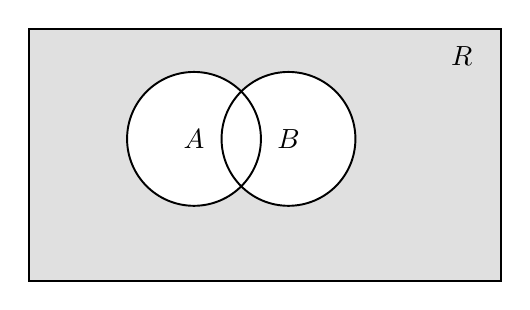
\begin{tikzpicture}[scale=1,line width=0.7pt]
\fill[black!12] (0,0) rectangle (6,3.2);
\fill[white] (2.1,1.8) circle (0.85);
\fill[white] (3.3,1.8) circle (0.85);
\draw (0,0) rectangle (6,3.2);
\draw (2.1,1.8) circle (0.85);
\draw (3.3,1.8) circle (0.85);
\node at (2.1,1.8) {$A$};
\node at (3.3,1.8) {$B$};
\node at (5.5,2.85) {$R$};
\end{tikzpicture}
\end{center}

（1）若集合 $C$ 表示图中阴影部分，用集合的运算式表示 $C$.

（2）求集合 $C$.

\ansspace*[12]

\ifanswer
\solbegin
\stepm{（1）}{由韦恩图得 $C=\overline{A\cup B}$.}
\stepm{（2）}{解 $\dfrac{x+1}{x-2}<-1$，则 $\dfrac{x+1}{x-2}+1<0$，即 $\dfrac{2x-1}{x-2}<0$，解得 $\dfrac12<x<2$，}
\step{故 $B=\left\{x\left|\dfrac12<x<2\right.\right\}$，所以 $A\cup B=\{x\mid-3\leqslant x<2\}$，}
\step{所以 $C=\overline{A\cup B}=\{x\mid x<-3\ \text{或}\ x\geqslant2\}$.}
\solend
\fi

\item 已知集合 $A=\{x\mid x^2-6x+8<0\}$，集合 $B=\{x\mid3m<x<1-m\}$.

（1）命题 $p:x\in A$，命题 $q:x\in B$，若 $p$ 是 $q$ 的充分条件，求实数 $m$ 的取值范围.

（2）若 $A\cap B=\varnothing$，求实数 $m$ 的取值范围.

\ansspace*[12]

\ifanswer
\solbegin
\stepm{（1）}{$x^2-6x+8<0\Rightarrow2<x<4\Rightarrow A=\{x\mid2<x<4\}$.}
\step{若 $p$ 是 $q$ 的充分条件，则 $A\subseteq B$，结合 $B$ 为非空集合，得 $\begin{cases}3m<1-m\\ 3m\leqslant2\\ 1-m\geqslant4\end{cases}$，}
\step{解得 $m\leqslant-3$，故 $m$ 的取值范围是 $(-\infty,-3]$；}
\stepm{（2）}{当 $B=\varnothing$ 时，$3m\geqslant1-m$，解得 $m\geqslant\dfrac14$，满足 $A\cap B=\varnothing$；}
\step{当 $B\neq\varnothing$ 时，$3m<1-m$ 即 $m<\dfrac14$，}
\step{要使交集为空，则 $1-m\leqslant2$ 或 $3m\geqslant4$，解得 $m\geqslant-1$，}
\step{结合 $m<\dfrac14$，得 $-1\leqslant m<\dfrac14$.}
\step{综上，$m\geqslant-1$，即 $m$ 的取值范围是 $[-1,+\infty)$.}
\solend
\fi

\item 设某企业每月生产电机 $x$ 台，根据企业月度报表知，每月总产值 $m$（万元）与总支出 $n$（万元）近似地满足下列关系：$m=\dfrac92x-\dfrac14$，$n=-\dfrac14x^2+5x+\dfrac74$，当 $m-n\geqslant0$ 时，称不亏损企业；当 $m-n<0$ 时，称亏损企业，且 $n-m$ 为亏损额.

（1）企业要成为不亏损企业，每月至少要生产多少台电机？

（2）当月总产值为多少时，企业亏损最严重，最大亏损额为多少？

\ansspace*[12]

\ifanswer
\solbegin
\stepm{（1）}{由题意得 $m-n\geqslant0$，即 $\dfrac92x-\dfrac14\geqslant-\dfrac14x^2+5x+\dfrac74$，}
\step{整理得 $x^2-2x-8\geqslant0$，解得 $x\geqslant4$ 或 $x\leqslant-2$（舍），}
\step{所以企业要成为不亏损企业，每月至少要生产 $4$ 台电机；}
\stepm{（2）}{由（1）得当 $0<x<4$ 时企业亏损，}
\step{亏损额 $n-m=\left(-\dfrac14x^2+5x+\dfrac74\right)-\left(\dfrac92x-\dfrac14\right)=-\dfrac14(x-1)^2+\dfrac94$，}
\step{所以当 $x=1$ 时，$n-m$ 取最大值 $\dfrac94$，}
\step{答：当月总产值为 $1$ 台时，企业亏损最严重，最大亏损额为 $\dfrac94$ 万元.}
\solend
\fi

\item 已知 $x_1$、$x_2$ 是一元二次方程 $4kx^2-4kx+k+1=0(k\neq0)$ 的两个实数根.

（1）是否存在实数 $k$，使 $x_1^2+x_2^2=\dfrac14$ 成立？若存在，求出 $k$ 的值，若不存在，请说明理由；

（2）是否存在整数 $k$，使 $\dfrac{x_1}{x_2}+\dfrac{x_2}{x_1}-2$ 的值为整数？若存在，求出 $k$ 的值，若不存在，请说明理由.

\ansspace*[14]

\ifanswer
\solbegin
\stepm{（1）}{因为 $x_1$、$x_2$ 是一元二次方程 $4kx^2-4kx+k+1=0(k\neq0)$ 的两个实数根，}
\step{所以 $\Delta=(-4k)^2-4\times4k(k+1)\geqslant0$，解得 $k\leqslant0$，}
\step{由韦达定理得 $\begin{cases}x_1+x_2=1\\ x_1x_2=\dfrac{k+1}{4k}\end{cases}$，}
\step{则 $x_1^2+x_2^2=(x_1+x_2)^2-2x_1x_2=\dfrac14$，}
\step{即 $1-2\times\dfrac{k+1}{4k}=\dfrac14$，解得 $k=2$，因为 $k\leqslant0$，所以不存在实数 $k$.}
\stepm{（2）}{$\dfrac{x_1}{x_2}+\dfrac{x_2}{x_1}-2=\dfrac{x_1^2+x_2^2}{x_1x_2}-2=\dfrac{(x_1+x_2)^2-2x_1x_2}{x_1x_2}-2=\dfrac{(x_1+x_2)^2}{x_1x_2}-4$}
\step{$=\dfrac{1}{\dfrac{k+1}{4k}}-4=\dfrac{4k}{k+1}-4=\dfrac{4k-4(k+1)}{k+1}=\dfrac{-4}{k+1}$，}
\step{由于 $\dfrac{x_1}{x_2}+\dfrac{x_2}{x_1}-2$ 的值为整数，即 $\dfrac{-4}{k+1}$ 的值为整数，}
\step{所以 $k+1$ 只能取 $\pm1$、$\pm2$、$\pm4$，}
\step{又 $k\leqslant0$，所以当 $k+1=\pm1$ 时，得出 $k=0$（舍）或 $k=-2$，}
\step{当 $k+1=\pm2$ 时，得出 $k=1$（舍）或 $k=-3$，}
\step{当 $k+1=\pm4$ 时，得出 $k=3$（舍）或 $k=-5$，}
\step{综上所述，若 $\dfrac{x_1}{x_2}+\dfrac{x_2}{x_1}-2$ 的值为整数，则 $k$ 的值为 $-2$ 或 $-3$ 或 $-5$.}
\solend
\fi

\item 已知集合 $A=\{a_1,a_2,\cdots,a_n\}(n\geqslant3)$，其中 $a_m\in\Z(m=1,2,\cdots,n)$. 若 $A$ 的子集 $T=\{a_i,a_j,a_k\}$ 满足 $2a_k=a_i+a_j$，则称 $T$ 具有性质 $P$. $A$ 的所有具有性质 $P$ 的子集 $T$ 的个数记为 $card_A(T)$.

（1）当 $A=\{4,-1,-2,1,-5\}$ 时，写出 $A$ 的所有具有性质 $P$ 的子集 $T$；

（2）当 $n=4$ 时，若 $a_1<a_2<a_3<a_4$，且 $card_A(T)=2$，证明：数对 $a_1$、$a_3$ 和 $a_2$、$a_4$ 中至少有一对中的两数奇偶性相同；

（3）当 $n=9$ 时，求 $card_A(T)$ 的最大值.

\ansspace*[14]

\ifanswer
\solbegin
\stepm{（1）}{集合 $A=\{4,-1,-2,1,-5\}$，元素按从小到大排列为 $-5$、$-2$、$-1$、$1$、$4$，}
\step{满足 $2a_k=a_i+a_j$ 的三元子集 $T$ 需满足其中一个元素是另外两个的平均数，}
\step{对于 $-5,-2,1$：$2\times(-2)=-4=-5+1$，满足条件，故 $T=\{-5,-2,1\}$，}
\step{对于 $-2,1,4$：$2\times1=2=-2+4$，满足条件，故 $T=\{-2,1,4\}$，}
\step{因此满足的子集有 $\{-5,-2,1\}$ 和 $\{-2,1,4\}$.}
\stepm{（2）}{假设数对 $(a_1,a_3)$ 和 $(a_2,a_4)$ 的两数奇偶性均不同，}
\step{即 $a_1$ 与 $a_3$ 一奇一偶，故 $a_1+a_3$ 为奇数，}
\step{$a_2$ 与 $a_4$ 一奇一偶，故 $a_2+a_4$ 为奇数，}
\step{集合 $A=\{a_1,a_2,a_3,a_4\}$ 的三元子集共 $\mathrm{C}_4^3=4$ 个：}
\step{$\{a_1,a_2,a_3\}$：若满足 $2a_2=a_1+a_3$，左边为偶数，右边为奇数，矛盾，故不满足；}
\step{$\{a_2,a_3,a_4\}$：若满足 $2a_3=a_2+a_4$，左边为偶数，右边为奇数，矛盾，故不满足；}
\step{$\{a_1,a_2,a_4\}$：需 $2a_2=a_1+a_4$；}
\step{$\{a_1,a_3,a_4\}$：需 $2a_3=a_1+a_4$.}
\step{若这两个子集都满足，则 $2a_2=2a_3\Rightarrow a_2=a_3$，与 $a_2<a_3$ 矛盾，}
\step{因此最多只有 $1$ 个子集满足条件，与 $card_A(T)=2$ 矛盾，故假设不成立，}
\step{即数对 $(a_1,a_3)$ 和 $(a_2,a_4)$ 中至少有一对的两数奇偶性相同.}
\stepm{（3）}{要最大化 $card_A(T)$，}
\step{集合 $A$ 应包含尽可能多的三元等差数列（即长度为 $3$ 的等差数列），}
\step{当 $A$ 为公差为 $1$ 的等差数列（如 $A=\{0,1,2,\cdots,8\}$）时，}
\step{三元等差数列的个数最多，}
\step{对于集合 $\{0,1,2,\cdots,8\}$，计算三元等差数列个数：}
\step{公差 $d=1$：$\{0,1,2\},\{1,2,3\},\cdots,\{6,7,8\}$，共 $7$ 个；}
\step{公差 $d=2$：$\{0,2,4\},\{1,3,5\},\cdots,\{4,6,8\}$，共 $5$ 个；}
\step{公差 $d=3$：$\{0,3,6\},\{1,4,7\},\{2,5,8\}$，共 $3$ 个；}
\step{公差 $d=4$：$\{0,4,8\}$，共 $1$ 个；}
\step{总个数为 $7+5+3+1=16$.}
\solend
\fi

\end{enumerate}

\end{document}
"
%
% 原始材料：微信公众号“魔都数学加油站”文章，连载“27学年高一89”；
% 原文标题“27学年高一89——2026-2027年上海市宝山中学高一上10月月考”；
% 原文链接：https://mp.weixin.qq.com/s/DZ-Q-hfS4UulNW_vGWrZXw。
% 正文为 10 张 PNG 页（`原图/高一89_宝山中学_10月月考/01..10.png`），
% 尺寸混排（第 6 页为 2560×3620，其余为 4762×6735），均按页序读取。
%
% 篇幅与题号：原卷自第 3 题起编号（第 1、2 题不在原文内）。填空题 3—12（10 题）、
% 选择题 13—16（4 题）、解答题 17—21（5 题），共 19 题。
%
% 讲评版：第 4 题只印【答案】（“$x\leqslant2$ 或 $y\leqslant2$”），本稿只给 \ans{}；
% 其余 18 题印【解析】，其中选择题答案在解析末句“故选 C／B／A／A”。
% 第 17 题题干带一幅韦恩图（全集 $R$、集合 $A$、$B$ 与阴影部分），三版都出。
%
% 副标题：原卷未印副标题。本稿按内容标作“集合与常用逻辑用语、不等式”。
%
% 原卷笔误/存疑（均照录未改，正文对应处另有 % 注）：
%   ① 第 8 题题干“$k\in R$”与第 12 题“$n\in N$”按原卷用斜体字母排，本稿沿用
%      $\R$、$\N$ 记号（见“排版差异”③），此处不再视为笔误；
%   ② 第 9 题解析“故 $a$ 的取值范围是 $a<-1$ 或 $\dfrac13<a<\dfrac12$”，未把
%      $a<-1$ 写成区间，与同题前两行的写法不统一，属原卷写法，照录；
%   ③ 第 20 题 (1) 由 $\Delta\geqslant0$ 得“$k\leqslant0$”，与题设 $k\neq0$ 合看
%      应为 $k<0$；原卷写 $k\leqslant0$ 并以之舍去 $k=2$，结论不变，照录。
%
% 与原卷的排版差异：
%   ① 原卷每题下直接印【答案】/【解析】，本稿按全稿惯例将答案与解析置于答案版；
%   ② 原卷未印副标题，本稿补出；填空横线统一排 \blankline[4.4em]；
%   ③ 原卷数集记号排斜体 $R$、$Z$、$N$，本稿按全稿惯例改用 $\R$、$\Z$、$\N$；
%   ④ 第 17—21 题的子问用行内“（1）（2）（3）”段，解析中的子问标号用 \stepm；
%   ⑤ 解答题按惯例加 \ansspace；选择题括号排 \mbox{（\quad）}；
%   ⑥ 第 17 题的韦恩图原卷排在题干右侧、文字绕排，本稿改排为题干后的居中图
%      （TikZ 重绘：原图该处有公众号粉色水印斜压，按原图布局重绘，标注一致）。
%
% 行数核对：逐题数 \step/\stepm 条数，合计 119 条（Q3：2；Q4：0；Q5：3；Q6：4；
% Q7：2；Q8：3；Q9：4；Q10：5；Q11：8；Q12：4；Q13：5；Q14：7；Q15：9；Q16：5；
% Q17：4；Q18：8；Q19：7；Q20：13；Q21：26）。第 4 题只印【答案】，不计入 \step 账。
% 原卷解析的换行按语意合并，未逐行强拆。
%
\documentclass[a4paper,11pt]{article}
\usepackage{common}

\begin{document}

\examtitlest[7]{2026--2027 年宝山中学高一上 10 月月考}{集合与常用逻辑用语、不等式}

\bigsec{一、填空题}

\begin{enumerate}
\setcounter{enumi}{2}

\item 满足 $\{1,2\}\subseteq A\subseteq\{1,2,3,4,5\}$ 的集合共 $A$ 有\blankline[4.4em]个.

\ifanswer
\solbegin
\step{由题意得 $A=\{1,2\}$ 与 $\{3,4,5\}$ 的非空子集的并集，}
\step{而 $\{3,4,5\}$ 的子集有 $2^3=8$ 个，所以满足条件的 $A$ 有 $8$ 个.}
\solend
\fi

\item 用反证法证明命题：“若 $x+y>4$，则 $x>2$ 且 $y>2$”时，第一步应该假设\blankline[4.4em].

\ifanswer
\ans{$x\leqslant2$ 或 $y\leqslant2$}
\fi

\item 已知等式 $2x^2+3x+5=a(2x+1)(x+1)+c$ 恒成立，则 $a-c$ 的值为\blankline[4.4em].

\ifanswer
\solbegin
\step{因为 $2x^2+3x+5=a(2x+1)(x+1)+c$ 恒成立，}
\step{所以 $2x^2+3x+5=2ax^2+3ax+a+c$ 恒成立，}
\step{则 $\begin{cases}2=2a\\ 3=3a\\ 5=a+c\end{cases}$，得 $a=1$，$c=4$，所以 $a-c=-3$.}
\solend
\fi

\item 不等式 $\lvert3x-1\rvert<x$ 的解集\blankline[4.4em].

\ifanswer
\solbegin
\step{当 $x\leqslant0$ 时，不等式的解集为 $\varnothing$，}
\step{当 $x>0$ 时，$\lvert3x-1\rvert<x$，即 $(3x-1)^2<x^2$，}
\step{整理得 $8x^2-6x+1<0$，$(2x-1)(4x-1)<0$，解得 $\dfrac14<x<\dfrac12$，满足 $x>0$.}
\step{故解集为 $\left(\dfrac14,\dfrac12\right)$.}
\solend
\fi

\item 比较两个代数式的大小关系：$x^2+2y^2$\blankline[3em]$2xy+2y-1$.

\ifanswer
\solbegin
\step{$x^2+2y^2-(2xy+2y-1)=x^2-2xy+y^2+y^2-2y+1$}
\step{$=(x-y)^2+(y-1)^2\geqslant0$，所以 $x^2+2y^2\geqslant2xy+2y-1$.}
\solend
\fi

\item $k\in\R$，关于 $x$ 的不等式 $x^2+\sqrt2kx+2>0$ 的解集为全体实数，则 $k$ 的取值范围是\blankline[4.4em].

\ifanswer
\solbegin
\step{因为关于 $x$ 的不等式 $x^2+\sqrt2kx+2>0$ 的解集为全体实数，}
\step{所以 $\Delta=(\sqrt2k)^2-4\times1\times2=2k^2-8<0$，解得 $-2<k<2$，}
\step{即实数 $k$ 的取值范围是 $(-2,2)$.}
\solend
\fi

\item 在平面直角坐标系内，点 $\left(2a-1,\dfrac{3a-1}{a+1}\right)$ 在第二象限，则 $a$ 的取值范围是\blankline[4.4em].

\ifanswer
\solbegin
\step{由题意得 $\begin{cases}2a-1<0\\[0.2em]\dfrac{3a-1}{a+1}>0\end{cases}$，}
\step{由 $2a-1<0$，解得 $a<\dfrac12$；}
\step{由 $\dfrac{3a-1}{a+1}>0$，解得 $a<-1$ 或 $a>\dfrac13$；}
\step{故 $a$ 的取值范围是 $a<-1$ 或 $\dfrac13<a<\dfrac12$.}
\solend
\fi

\item 设集合 $A=\{x\mid x^2+x-6=0\}$，集合 $B=\{x\mid mx+1=0\}$，且 $A\cup B=A$，则 $m$ 的值组成的集合是\blankline[4.4em].

\ifanswer
\solbegin
\step{由题意得 $A=\{x\mid x^2+x-6=0\}=\{-3,2\}$，}
\step{由 $A\cup B=A$，得 $B\subseteq A$，}
\step{当 $m=0$ 时，$B=\varnothing$，满足题意，}
\step{当 $m\neq0$ 时，$B=\left\{-\dfrac1m\right\}$，所以 $-\dfrac1m=2$ 或 $-\dfrac1m=-3$，所以 $m=-\dfrac12$ 或 $m=\dfrac13$，}
\step{综上所述，$m$ 的值组成的集合是 $\left\{0,-\dfrac12,\dfrac13\right\}$.}
\solend
\fi

\item 甲、乙两人解关于 $x$ 的不等式 $x^2+bx+c<0$，甲写错了 $b$，正确计算后得到的解为 $\{x\mid1<x<2\}$；乙写错了 $c$，正确计算后得到的解为 $\{x\mid-4<x<1\}$. 那么不等式 $\dfrac{bx+c}{x-2}<0$ 的解为\blankline[4.4em].

\ifanswer
\solbegin
\step{由 $x^2+bx+c<0$ 的解为 $\{x\mid1<x<2\}$，}
\step{则 $1$ 和 $2$ 是方程 $x^2+bx+c=0$ 的两个根，}
\step{甲写错了 $b$，但 $c$ 是正确的，所以 $c=1\times2=2$；}
\step{由 $x^2+bx+c<0$ 的解为 $\{x\mid-4<x<1\}$，}
\step{则 $-4$ 和 $1$ 是方程 $x^2+bx+c=0$ 的两个根，}
\step{乙写错了 $c$，但 $b$ 是正确的，所以 $-b=-4+1=-3$，即 $b=3$.}
\step{由 $\dfrac{bx+c}{x-2}<0$，得 $\dfrac{3x+2}{x-2}<0$，即 $(3x+2)(x-2)<0$，解得 $-\dfrac23<x<2$，}
\step{所以不等式 $\dfrac{bx+c}{x-2}<0$ 的解为 $\left\{x\left|-\dfrac23<x<2\right.\right\}$.}
\solend
\fi

\item 已知集合 $M$ 的元素均为正整数，定义集合 $M$ 的“变项和”为：将 $M$ 中每个元素 $m$ 都乘以 $(-1)^m$ 后再求和. 若集合 $A=\{n\mid1\leqslant n\leqslant10,n\in\N\}$，则集合 $A$ 的所有非空子集的“变项和”的总和为\blankline[4.4em].

\ifanswer
\solbegin
\step{$A$ 集合的所有非空子集中，每个元素出现的次数都是 $(2^{10}-1)-(2^9-1)=2^9$，}
\step{则集合 $A$ 的所有非空子集的“变项和”的总和}
\step{为 $1\times(-1)^1\times2^9+2\times(-1)^2\times2^9+\cdots+10\times(-1)^{10}\times2^9$}
\step{$=(-1+2-3+4-\cdots-9+10)\times2^9=5\times2^9=2560$.}
\solend
\fi

\end{enumerate}

\bigsec{二、选择题}

\begin{enumerate}
\setcounter{enumi}{12}

\item 下列命题中正确的是\mbox{（\quad）}

\keepwithprev
A. 若 $a>b$，则 $\dfrac1a<\dfrac1b$\qquad B. 若 $a>b$，则 $a^2>b^2$

C. 若 $a>\lvert b\rvert$，则 $a>b$\qquad D. 若 $a>b$，则 $ac^2>bc^2$

\ifanswer
\solbegin
\step{对于 $AB$ 选项，取 $a=1$，$b=-1$，$a>b$，$\dfrac1a>\dfrac1b$，$a^2=b^2$，}
\step{所以 $AB$ 选项错误；}
\step{对于 $C$ 选项，由 $a>\lvert b\rvert$，$\lvert b\rvert\geqslant b$，得 $a>b$，所以 $C$ 选项正确；}
\step{对于 $D$ 选项，取 $c=0$，则 $ac^2=0=bc^2$，所以 $D$ 选项错误.}
\step{故选 $C$.}
\solend
\fi

\item 下面关于集合的表示正确的个数是\mbox{（\quad）}

①$\{1,2,3\}=\{3,2,1\}$；\quad ②$\{(x,y)\mid x-y=1\}=\{y\mid y=x-1\}$；

③$\{x\mid x\geqslant2,x\in\N\}=\{y\mid y\geqslant2,y\in\Z\}$；\quad ④$\{x\mid x+2y=1\}\neq\left\{y\left|y=-\dfrac12x+\dfrac12\right.\right\}$.

\keepwithprev
A. $1$\qquad B. $2$\qquad C. $3$\qquad D. $4$

\ifanswer
\solbegin
\step{对于①，由元素的无序性得①正确；}
\step{对于②，$\{(x,y)\mid x-y=1\}$ 表示点集，$\{y\mid y=x-1\}$ 表示数集，故②错误；}
\step{对于③，$\{x\mid x\geqslant2,x\in\N\}$ 表示大于等于 $2$ 的整数，}
\step{$\{y\mid y\geqslant2,y\in\Z\}$ 也表示大于等于 $2$ 的整数，故③正确；}
\step{对于④，$\{x\mid x+2y=1\}=\R$，$\left\{y\left|y=-\dfrac12x+\dfrac12\right.\right\}=\R$，}
\step{所以 $\{x\mid x+2y=1\}=\left\{y\left|y=-\dfrac12x+\dfrac12\right.\right\}$，故④错误，}
\step{所以正确的个数是 $2$ 个. 故选 $B$.}
\solend
\fi

\item 已知命题 $P$：方程 $ax^2+bx+c=0$ 有两个不相等实根；命题 $Q$：不等式 $ax^2+bx+c>0$ 与 $ax^2+bx+c<0$ 均有解，则命题 $P$ 成立是命题 $Q$ 成立的\mbox{（\quad）}条件.

\keepwithprev
A. 充分非必要条件\qquad B. 必要非充分条件

C. 充要条件\qquad D. 既非充分又非必要条件

\ifanswer
\solbegin
\step{若 $P$ 成立，即方程 $ax^2+bx+c=0$ 有两个不相等实根，}
\step{此时 $\begin{cases}a\neq0\\ \Delta=b^2-4ac>0\end{cases}$；}
\step{若 $Q$ 成立，即不等式 $ax^2+bx+c>0$ 与 $ax^2+bx+c<0$ 均有解，有两种情况：}
\step{①不等式是一元二次不等式，}
\step{此时不等式所对应的二次函数的图像与 $x$ 轴有两个交点，}
\step{满足 $\begin{cases}a\neq0\\ \Delta=b^2-4ac>0\end{cases}$；}
\step{②不等式是一元一次不等式，此时 $\begin{cases}a=0\\ b\neq0\end{cases}$，}
\step{因此，由 $P$ 能推出 $Q$ 成立，但是由 $Q$ 不能推出 $P$ 成立，}
\step{即 $P$ 是 $Q$ 的充分非必要条件. 故选 $A$.}
\solend
\fi

\item 甲、乙同去加油站加油两次，两次汽油单价分别为 $x$、$y$ 元/升（$x\neq y$）. 甲每次加固定金额的油，乙每次加固定体积的油. 哪种方式更经济实惠呢？\mbox{（\quad）}

\keepwithprev
A. 加固定金额的方式\qquad B. 加固定体积的方式

C. 两种方案一样\qquad D. 要视具体价格而定

\ifanswer
\solbegin
\step{设两次加油的油价分别为 $x$、$y$（$x$、$y>0$，且 $x\neq y$），}
\step{乙每次加油的量为 $a$（$a>0$）；甲每次加油的钱数为 $b$（$b>0$），}
\step{则乙平均油价为 $\dfrac{ax+ay}{2a}=\dfrac{x+y}{2}$，甲平均油价为 $\dfrac{2b}{\dfrac bx+\dfrac by}=\dfrac2{\dfrac1x+\dfrac1y}=\dfrac{2xy}{x+y}$，}
\step{因为 $x\neq y$，所以 $\dfrac{x+y}{2}-\dfrac{2xy}{x+y}=\dfrac{(x-y)^2}{2(x+y)}>0$，所以 $\dfrac{x+y}{2}>\dfrac{2xy}{x+y}$，}
\step{即甲方案更经济. 故选 $A$.}
\solend
\fi

\end{enumerate}

\bigsec{三、解答题}

\begin{enumerate}
\setcounter{enumi}{16}

\item 已知全集 $U=\R$，集合 $A=\{x\mid-3\leqslant x\leqslant1\}$，$B=\left\{x\left|\dfrac{x+1}{x-2}<-1\right.\right\}$.

\begin{center}
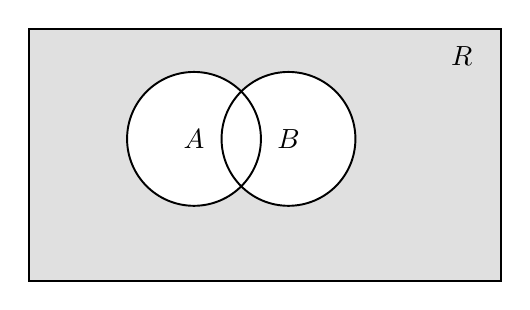
\begin{tikzpicture}[scale=1,line width=0.7pt]
\fill[black!12] (0,0) rectangle (6,3.2);
\fill[white] (2.1,1.8) circle (0.85);
\fill[white] (3.3,1.8) circle (0.85);
\draw (0,0) rectangle (6,3.2);
\draw (2.1,1.8) circle (0.85);
\draw (3.3,1.8) circle (0.85);
\node at (2.1,1.8) {$A$};
\node at (3.3,1.8) {$B$};
\node at (5.5,2.85) {$R$};
\end{tikzpicture}
\end{center}

（1）若集合 $C$ 表示图中阴影部分，用集合的运算式表示 $C$.

（2）求集合 $C$.

\ansspace*[12]

\ifanswer
\solbegin
\stepm{（1）}{由韦恩图得 $C=\overline{A\cup B}$.}
\stepm{（2）}{解 $\dfrac{x+1}{x-2}<-1$，则 $\dfrac{x+1}{x-2}+1<0$，即 $\dfrac{2x-1}{x-2}<0$，解得 $\dfrac12<x<2$，}
\step{故 $B=\left\{x\left|\dfrac12<x<2\right.\right\}$，所以 $A\cup B=\{x\mid-3\leqslant x<2\}$，}
\step{所以 $C=\overline{A\cup B}=\{x\mid x<-3\ \text{或}\ x\geqslant2\}$.}
\solend
\fi

\item 已知集合 $A=\{x\mid x^2-6x+8<0\}$，集合 $B=\{x\mid3m<x<1-m\}$.

（1）命题 $p:x\in A$，命题 $q:x\in B$，若 $p$ 是 $q$ 的充分条件，求实数 $m$ 的取值范围.

（2）若 $A\cap B=\varnothing$，求实数 $m$ 的取值范围.

\ansspace*[12]

\ifanswer
\solbegin
\stepm{（1）}{$x^2-6x+8<0\Rightarrow2<x<4\Rightarrow A=\{x\mid2<x<4\}$.}
\step{若 $p$ 是 $q$ 的充分条件，则 $A\subseteq B$，结合 $B$ 为非空集合，得 $\begin{cases}3m<1-m\\ 3m\leqslant2\\ 1-m\geqslant4\end{cases}$，}
\step{解得 $m\leqslant-3$，故 $m$ 的取值范围是 $(-\infty,-3]$；}
\stepm{（2）}{当 $B=\varnothing$ 时，$3m\geqslant1-m$，解得 $m\geqslant\dfrac14$，满足 $A\cap B=\varnothing$；}
\step{当 $B\neq\varnothing$ 时，$3m<1-m$ 即 $m<\dfrac14$，}
\step{要使交集为空，则 $1-m\leqslant2$ 或 $3m\geqslant4$，解得 $m\geqslant-1$，}
\step{结合 $m<\dfrac14$，得 $-1\leqslant m<\dfrac14$.}
\step{综上，$m\geqslant-1$，即 $m$ 的取值范围是 $[-1,+\infty)$.}
\solend
\fi

\item 设某企业每月生产电机 $x$ 台，根据企业月度报表知，每月总产值 $m$（万元）与总支出 $n$（万元）近似地满足下列关系：$m=\dfrac92x-\dfrac14$，$n=-\dfrac14x^2+5x+\dfrac74$，当 $m-n\geqslant0$ 时，称不亏损企业；当 $m-n<0$ 时，称亏损企业，且 $n-m$ 为亏损额.

（1）企业要成为不亏损企业，每月至少要生产多少台电机？

（2）当月总产值为多少时，企业亏损最严重，最大亏损额为多少？

\ansspace*[12]

\ifanswer
\solbegin
\stepm{（1）}{由题意得 $m-n\geqslant0$，即 $\dfrac92x-\dfrac14\geqslant-\dfrac14x^2+5x+\dfrac74$，}
\step{整理得 $x^2-2x-8\geqslant0$，解得 $x\geqslant4$ 或 $x\leqslant-2$（舍），}
\step{所以企业要成为不亏损企业，每月至少要生产 $4$ 台电机；}
\stepm{（2）}{由（1）得当 $0<x<4$ 时企业亏损，}
\step{亏损额 $n-m=\left(-\dfrac14x^2+5x+\dfrac74\right)-\left(\dfrac92x-\dfrac14\right)=-\dfrac14(x-1)^2+\dfrac94$，}
\step{所以当 $x=1$ 时，$n-m$ 取最大值 $\dfrac94$，}
\step{答：当月总产值为 $1$ 台时，企业亏损最严重，最大亏损额为 $\dfrac94$ 万元.}
\solend
\fi

\item 已知 $x_1$、$x_2$ 是一元二次方程 $4kx^2-4kx+k+1=0(k\neq0)$ 的两个实数根.

（1）是否存在实数 $k$，使 $x_1^2+x_2^2=\dfrac14$ 成立？若存在，求出 $k$ 的值，若不存在，请说明理由；

（2）是否存在整数 $k$，使 $\dfrac{x_1}{x_2}+\dfrac{x_2}{x_1}-2$ 的值为整数？若存在，求出 $k$ 的值，若不存在，请说明理由.

\ansspace*[14]

\ifanswer
\solbegin
\stepm{（1）}{因为 $x_1$、$x_2$ 是一元二次方程 $4kx^2-4kx+k+1=0(k\neq0)$ 的两个实数根，}
\step{所以 $\Delta=(-4k)^2-4\times4k(k+1)\geqslant0$，解得 $k\leqslant0$，}
\step{由韦达定理得 $\begin{cases}x_1+x_2=1\\ x_1x_2=\dfrac{k+1}{4k}\end{cases}$，}
\step{则 $x_1^2+x_2^2=(x_1+x_2)^2-2x_1x_2=\dfrac14$，}
\step{即 $1-2\times\dfrac{k+1}{4k}=\dfrac14$，解得 $k=2$，因为 $k\leqslant0$，所以不存在实数 $k$.}
\stepm{（2）}{$\dfrac{x_1}{x_2}+\dfrac{x_2}{x_1}-2=\dfrac{x_1^2+x_2^2}{x_1x_2}-2=\dfrac{(x_1+x_2)^2-2x_1x_2}{x_1x_2}-2=\dfrac{(x_1+x_2)^2}{x_1x_2}-4$}
\step{$=\dfrac{1}{\dfrac{k+1}{4k}}-4=\dfrac{4k}{k+1}-4=\dfrac{4k-4(k+1)}{k+1}=\dfrac{-4}{k+1}$，}
\step{由于 $\dfrac{x_1}{x_2}+\dfrac{x_2}{x_1}-2$ 的值为整数，即 $\dfrac{-4}{k+1}$ 的值为整数，}
\step{所以 $k+1$ 只能取 $\pm1$、$\pm2$、$\pm4$，}
\step{又 $k\leqslant0$，所以当 $k+1=\pm1$ 时，得出 $k=0$（舍）或 $k=-2$，}
\step{当 $k+1=\pm2$ 时，得出 $k=1$（舍）或 $k=-3$，}
\step{当 $k+1=\pm4$ 时，得出 $k=3$（舍）或 $k=-5$，}
\step{综上所述，若 $\dfrac{x_1}{x_2}+\dfrac{x_2}{x_1}-2$ 的值为整数，则 $k$ 的值为 $-2$ 或 $-3$ 或 $-5$.}
\solend
\fi

\item 已知集合 $A=\{a_1,a_2,\cdots,a_n\}(n\geqslant3)$，其中 $a_m\in\Z(m=1,2,\cdots,n)$. 若 $A$ 的子集 $T=\{a_i,a_j,a_k\}$ 满足 $2a_k=a_i+a_j$，则称 $T$ 具有性质 $P$. $A$ 的所有具有性质 $P$ 的子集 $T$ 的个数记为 $card_A(T)$.

（1）当 $A=\{4,-1,-2,1,-5\}$ 时，写出 $A$ 的所有具有性质 $P$ 的子集 $T$；

（2）当 $n=4$ 时，若 $a_1<a_2<a_3<a_4$，且 $card_A(T)=2$，证明：数对 $a_1$、$a_3$ 和 $a_2$、$a_4$ 中至少有一对中的两数奇偶性相同；

（3）当 $n=9$ 时，求 $card_A(T)$ 的最大值.

\ansspace*[14]

\ifanswer
\solbegin
\stepm{（1）}{集合 $A=\{4,-1,-2,1,-5\}$，元素按从小到大排列为 $-5$、$-2$、$-1$、$1$、$4$，}
\step{满足 $2a_k=a_i+a_j$ 的三元子集 $T$ 需满足其中一个元素是另外两个的平均数，}
\step{对于 $-5,-2,1$：$2\times(-2)=-4=-5+1$，满足条件，故 $T=\{-5,-2,1\}$，}
\step{对于 $-2,1,4$：$2\times1=2=-2+4$，满足条件，故 $T=\{-2,1,4\}$，}
\step{因此满足的子集有 $\{-5,-2,1\}$ 和 $\{-2,1,4\}$.}
\stepm{（2）}{假设数对 $(a_1,a_3)$ 和 $(a_2,a_4)$ 的两数奇偶性均不同，}
\step{即 $a_1$ 与 $a_3$ 一奇一偶，故 $a_1+a_3$ 为奇数，}
\step{$a_2$ 与 $a_4$ 一奇一偶，故 $a_2+a_4$ 为奇数，}
\step{集合 $A=\{a_1,a_2,a_3,a_4\}$ 的三元子集共 $\mathrm{C}_4^3=4$ 个：}
\step{$\{a_1,a_2,a_3\}$：若满足 $2a_2=a_1+a_3$，左边为偶数，右边为奇数，矛盾，故不满足；}
\step{$\{a_2,a_3,a_4\}$：若满足 $2a_3=a_2+a_4$，左边为偶数，右边为奇数，矛盾，故不满足；}
\step{$\{a_1,a_2,a_4\}$：需 $2a_2=a_1+a_4$；}
\step{$\{a_1,a_3,a_4\}$：需 $2a_3=a_1+a_4$.}
\step{若这两个子集都满足，则 $2a_2=2a_3\Rightarrow a_2=a_3$，与 $a_2<a_3$ 矛盾，}
\step{因此最多只有 $1$ 个子集满足条件，与 $card_A(T)=2$ 矛盾，故假设不成立，}
\step{即数对 $(a_1,a_3)$ 和 $(a_2,a_4)$ 中至少有一对的两数奇偶性相同.}
\stepm{（3）}{要最大化 $card_A(T)$，}
\step{集合 $A$ 应包含尽可能多的三元等差数列（即长度为 $3$ 的等差数列），}
\step{当 $A$ 为公差为 $1$ 的等差数列（如 $A=\{0,1,2,\cdots,8\}$）时，}
\step{三元等差数列的个数最多，}
\step{对于集合 $\{0,1,2,\cdots,8\}$，计算三元等差数列个数：}
\step{公差 $d=1$：$\{0,1,2\},\{1,2,3\},\cdots,\{6,7,8\}$，共 $7$ 个；}
\step{公差 $d=2$：$\{0,2,4\},\{1,3,5\},\cdots,\{4,6,8\}$，共 $5$ 个；}
\step{公差 $d=3$：$\{0,3,6\},\{1,4,7\},\{2,5,8\}$，共 $3$ 个；}
\step{公差 $d=4$：$\{0,4,8\}$，共 $1$ 个；}
\step{总个数为 $7+5+3+1=16$.}
\solend
\fi

\end{enumerate}

\end{document}
"
% 紧凑版：xelatex "\def\iscompact{1}% 高一89_宝山中学_10月月考.tex
%   —— 高一上数学“2026-2027 年宝山中学高一上 10 月月考”（讲评版）
% 试卷版：xelatex 高一89_宝山中学_10月月考.tex
% 答案版：xelatex "\def\isanswer{1}% 高一89_宝山中学_10月月考.tex
%   —— 高一上数学“2026-2027 年宝山中学高一上 10 月月考”（讲评版）
% 试卷版：xelatex 高一89_宝山中学_10月月考.tex
% 答案版：xelatex "\def\isanswer{1}% 高一89_宝山中学_10月月考.tex
%   —— 高一上数学“2026-2027 年宝山中学高一上 10 月月考”（讲评版）
% 试卷版：xelatex 高一89_宝山中学_10月月考.tex
% 答案版：xelatex "\def\isanswer{1}\input{高一89_宝山中学_10月月考.tex}"
% 紧凑版：xelatex "\def\iscompact{1}\input{高一89_宝山中学_10月月考.tex}"
%
% 原始材料：微信公众号“魔都数学加油站”文章，连载“27学年高一89”；
% 原文标题“27学年高一89——2026-2027年上海市宝山中学高一上10月月考”；
% 原文链接：https://mp.weixin.qq.com/s/DZ-Q-hfS4UulNW_vGWrZXw。
% 正文为 10 张 PNG 页（`原图/高一89_宝山中学_10月月考/01..10.png`），
% 尺寸混排（第 6 页为 2560×3620，其余为 4762×6735），均按页序读取。
%
% 篇幅与题号：原卷自第 3 题起编号（第 1、2 题不在原文内）。填空题 3—12（10 题）、
% 选择题 13—16（4 题）、解答题 17—21（5 题），共 19 题。
%
% 讲评版：第 4 题只印【答案】（“$x\leqslant2$ 或 $y\leqslant2$”），本稿只给 \ans{}；
% 其余 18 题印【解析】，其中选择题答案在解析末句“故选 C／B／A／A”。
% 第 17 题题干带一幅韦恩图（全集 $R$、集合 $A$、$B$ 与阴影部分），三版都出。
%
% 副标题：原卷未印副标题。本稿按内容标作“集合与常用逻辑用语、不等式”。
%
% 原卷笔误/存疑（均照录未改，正文对应处另有 % 注）：
%   ① 第 8 题题干“$k\in R$”与第 12 题“$n\in N$”按原卷用斜体字母排，本稿沿用
%      $\R$、$\N$ 记号（见“排版差异”③），此处不再视为笔误；
%   ② 第 9 题解析“故 $a$ 的取值范围是 $a<-1$ 或 $\dfrac13<a<\dfrac12$”，未把
%      $a<-1$ 写成区间，与同题前两行的写法不统一，属原卷写法，照录；
%   ③ 第 20 题 (1) 由 $\Delta\geqslant0$ 得“$k\leqslant0$”，与题设 $k\neq0$ 合看
%      应为 $k<0$；原卷写 $k\leqslant0$ 并以之舍去 $k=2$，结论不变，照录。
%
% 与原卷的排版差异：
%   ① 原卷每题下直接印【答案】/【解析】，本稿按全稿惯例将答案与解析置于答案版；
%   ② 原卷未印副标题，本稿补出；填空横线统一排 \blankline[4.4em]；
%   ③ 原卷数集记号排斜体 $R$、$Z$、$N$，本稿按全稿惯例改用 $\R$、$\Z$、$\N$；
%   ④ 第 17—21 题的子问用行内“（1）（2）（3）”段，解析中的子问标号用 \stepm；
%   ⑤ 解答题按惯例加 \ansspace；选择题括号排 \mbox{（\quad）}；
%   ⑥ 第 17 题的韦恩图原卷排在题干右侧、文字绕排，本稿改排为题干后的居中图
%      （TikZ 重绘：原图该处有公众号粉色水印斜压，按原图布局重绘，标注一致）。
%
% 行数核对：逐题数 \step/\stepm 条数，合计 119 条（Q3：2；Q4：0；Q5：3；Q6：4；
% Q7：2；Q8：3；Q9：4；Q10：5；Q11：8；Q12：4；Q13：5；Q14：7；Q15：9；Q16：5；
% Q17：4；Q18：8；Q19：7；Q20：13；Q21：26）。第 4 题只印【答案】，不计入 \step 账。
% 原卷解析的换行按语意合并，未逐行强拆。
%
\documentclass[a4paper,11pt]{article}
\usepackage{common}

\begin{document}

\examtitlest[7]{2026--2027 年宝山中学高一上 10 月月考}{集合与常用逻辑用语、不等式}

\bigsec{一、填空题}

\begin{enumerate}
\setcounter{enumi}{2}

\item 满足 $\{1,2\}\subseteq A\subseteq\{1,2,3,4,5\}$ 的集合共 $A$ 有\blankline[4.4em]个.

\ifanswer
\solbegin
\step{由题意得 $A=\{1,2\}$ 与 $\{3,4,5\}$ 的非空子集的并集，}
\step{而 $\{3,4,5\}$ 的子集有 $2^3=8$ 个，所以满足条件的 $A$ 有 $8$ 个.}
\solend
\fi

\item 用反证法证明命题：“若 $x+y>4$，则 $x>2$ 且 $y>2$”时，第一步应该假设\blankline[4.4em].

\ifanswer
\ans{$x\leqslant2$ 或 $y\leqslant2$}
\fi

\item 已知等式 $2x^2+3x+5=a(2x+1)(x+1)+c$ 恒成立，则 $a-c$ 的值为\blankline[4.4em].

\ifanswer
\solbegin
\step{因为 $2x^2+3x+5=a(2x+1)(x+1)+c$ 恒成立，}
\step{所以 $2x^2+3x+5=2ax^2+3ax+a+c$ 恒成立，}
\step{则 $\begin{cases}2=2a\\ 3=3a\\ 5=a+c\end{cases}$，得 $a=1$，$c=4$，所以 $a-c=-3$.}
\solend
\fi

\item 不等式 $\lvert3x-1\rvert<x$ 的解集\blankline[4.4em].

\ifanswer
\solbegin
\step{当 $x\leqslant0$ 时，不等式的解集为 $\varnothing$，}
\step{当 $x>0$ 时，$\lvert3x-1\rvert<x$，即 $(3x-1)^2<x^2$，}
\step{整理得 $8x^2-6x+1<0$，$(2x-1)(4x-1)<0$，解得 $\dfrac14<x<\dfrac12$，满足 $x>0$.}
\step{故解集为 $\left(\dfrac14,\dfrac12\right)$.}
\solend
\fi

\item 比较两个代数式的大小关系：$x^2+2y^2$\blankline[3em]$2xy+2y-1$.

\ifanswer
\solbegin
\step{$x^2+2y^2-(2xy+2y-1)=x^2-2xy+y^2+y^2-2y+1$}
\step{$=(x-y)^2+(y-1)^2\geqslant0$，所以 $x^2+2y^2\geqslant2xy+2y-1$.}
\solend
\fi

\item $k\in\R$，关于 $x$ 的不等式 $x^2+\sqrt2kx+2>0$ 的解集为全体实数，则 $k$ 的取值范围是\blankline[4.4em].

\ifanswer
\solbegin
\step{因为关于 $x$ 的不等式 $x^2+\sqrt2kx+2>0$ 的解集为全体实数，}
\step{所以 $\Delta=(\sqrt2k)^2-4\times1\times2=2k^2-8<0$，解得 $-2<k<2$，}
\step{即实数 $k$ 的取值范围是 $(-2,2)$.}
\solend
\fi

\item 在平面直角坐标系内，点 $\left(2a-1,\dfrac{3a-1}{a+1}\right)$ 在第二象限，则 $a$ 的取值范围是\blankline[4.4em].

\ifanswer
\solbegin
\step{由题意得 $\begin{cases}2a-1<0\\[0.2em]\dfrac{3a-1}{a+1}>0\end{cases}$，}
\step{由 $2a-1<0$，解得 $a<\dfrac12$；}
\step{由 $\dfrac{3a-1}{a+1}>0$，解得 $a<-1$ 或 $a>\dfrac13$；}
\step{故 $a$ 的取值范围是 $a<-1$ 或 $\dfrac13<a<\dfrac12$.}
\solend
\fi

\item 设集合 $A=\{x\mid x^2+x-6=0\}$，集合 $B=\{x\mid mx+1=0\}$，且 $A\cup B=A$，则 $m$ 的值组成的集合是\blankline[4.4em].

\ifanswer
\solbegin
\step{由题意得 $A=\{x\mid x^2+x-6=0\}=\{-3,2\}$，}
\step{由 $A\cup B=A$，得 $B\subseteq A$，}
\step{当 $m=0$ 时，$B=\varnothing$，满足题意，}
\step{当 $m\neq0$ 时，$B=\left\{-\dfrac1m\right\}$，所以 $-\dfrac1m=2$ 或 $-\dfrac1m=-3$，所以 $m=-\dfrac12$ 或 $m=\dfrac13$，}
\step{综上所述，$m$ 的值组成的集合是 $\left\{0,-\dfrac12,\dfrac13\right\}$.}
\solend
\fi

\item 甲、乙两人解关于 $x$ 的不等式 $x^2+bx+c<0$，甲写错了 $b$，正确计算后得到的解为 $\{x\mid1<x<2\}$；乙写错了 $c$，正确计算后得到的解为 $\{x\mid-4<x<1\}$. 那么不等式 $\dfrac{bx+c}{x-2}<0$ 的解为\blankline[4.4em].

\ifanswer
\solbegin
\step{由 $x^2+bx+c<0$ 的解为 $\{x\mid1<x<2\}$，}
\step{则 $1$ 和 $2$ 是方程 $x^2+bx+c=0$ 的两个根，}
\step{甲写错了 $b$，但 $c$ 是正确的，所以 $c=1\times2=2$；}
\step{由 $x^2+bx+c<0$ 的解为 $\{x\mid-4<x<1\}$，}
\step{则 $-4$ 和 $1$ 是方程 $x^2+bx+c=0$ 的两个根，}
\step{乙写错了 $c$，但 $b$ 是正确的，所以 $-b=-4+1=-3$，即 $b=3$.}
\step{由 $\dfrac{bx+c}{x-2}<0$，得 $\dfrac{3x+2}{x-2}<0$，即 $(3x+2)(x-2)<0$，解得 $-\dfrac23<x<2$，}
\step{所以不等式 $\dfrac{bx+c}{x-2}<0$ 的解为 $\left\{x\left|-\dfrac23<x<2\right.\right\}$.}
\solend
\fi

\item 已知集合 $M$ 的元素均为正整数，定义集合 $M$ 的“变项和”为：将 $M$ 中每个元素 $m$ 都乘以 $(-1)^m$ 后再求和. 若集合 $A=\{n\mid1\leqslant n\leqslant10,n\in\N\}$，则集合 $A$ 的所有非空子集的“变项和”的总和为\blankline[4.4em].

\ifanswer
\solbegin
\step{$A$ 集合的所有非空子集中，每个元素出现的次数都是 $(2^{10}-1)-(2^9-1)=2^9$，}
\step{则集合 $A$ 的所有非空子集的“变项和”的总和}
\step{为 $1\times(-1)^1\times2^9+2\times(-1)^2\times2^9+\cdots+10\times(-1)^{10}\times2^9$}
\step{$=(-1+2-3+4-\cdots-9+10)\times2^9=5\times2^9=2560$.}
\solend
\fi

\end{enumerate}

\bigsec{二、选择题}

\begin{enumerate}
\setcounter{enumi}{12}

\item 下列命题中正确的是\mbox{（\quad）}

\keepwithprev
A. 若 $a>b$，则 $\dfrac1a<\dfrac1b$\qquad B. 若 $a>b$，则 $a^2>b^2$

C. 若 $a>\lvert b\rvert$，则 $a>b$\qquad D. 若 $a>b$，则 $ac^2>bc^2$

\ifanswer
\solbegin
\step{对于 $AB$ 选项，取 $a=1$，$b=-1$，$a>b$，$\dfrac1a>\dfrac1b$，$a^2=b^2$，}
\step{所以 $AB$ 选项错误；}
\step{对于 $C$ 选项，由 $a>\lvert b\rvert$，$\lvert b\rvert\geqslant b$，得 $a>b$，所以 $C$ 选项正确；}
\step{对于 $D$ 选项，取 $c=0$，则 $ac^2=0=bc^2$，所以 $D$ 选项错误.}
\step{故选 $C$.}
\solend
\fi

\item 下面关于集合的表示正确的个数是\mbox{（\quad）}

①$\{1,2,3\}=\{3,2,1\}$；\quad ②$\{(x,y)\mid x-y=1\}=\{y\mid y=x-1\}$；

③$\{x\mid x\geqslant2,x\in\N\}=\{y\mid y\geqslant2,y\in\Z\}$；\quad ④$\{x\mid x+2y=1\}\neq\left\{y\left|y=-\dfrac12x+\dfrac12\right.\right\}$.

\keepwithprev
A. $1$\qquad B. $2$\qquad C. $3$\qquad D. $4$

\ifanswer
\solbegin
\step{对于①，由元素的无序性得①正确；}
\step{对于②，$\{(x,y)\mid x-y=1\}$ 表示点集，$\{y\mid y=x-1\}$ 表示数集，故②错误；}
\step{对于③，$\{x\mid x\geqslant2,x\in\N\}$ 表示大于等于 $2$ 的整数，}
\step{$\{y\mid y\geqslant2,y\in\Z\}$ 也表示大于等于 $2$ 的整数，故③正确；}
\step{对于④，$\{x\mid x+2y=1\}=\R$，$\left\{y\left|y=-\dfrac12x+\dfrac12\right.\right\}=\R$，}
\step{所以 $\{x\mid x+2y=1\}=\left\{y\left|y=-\dfrac12x+\dfrac12\right.\right\}$，故④错误，}
\step{所以正确的个数是 $2$ 个. 故选 $B$.}
\solend
\fi

\item 已知命题 $P$：方程 $ax^2+bx+c=0$ 有两个不相等实根；命题 $Q$：不等式 $ax^2+bx+c>0$ 与 $ax^2+bx+c<0$ 均有解，则命题 $P$ 成立是命题 $Q$ 成立的\mbox{（\quad）}条件.

\keepwithprev
A. 充分非必要条件\qquad B. 必要非充分条件

C. 充要条件\qquad D. 既非充分又非必要条件

\ifanswer
\solbegin
\step{若 $P$ 成立，即方程 $ax^2+bx+c=0$ 有两个不相等实根，}
\step{此时 $\begin{cases}a\neq0\\ \Delta=b^2-4ac>0\end{cases}$；}
\step{若 $Q$ 成立，即不等式 $ax^2+bx+c>0$ 与 $ax^2+bx+c<0$ 均有解，有两种情况：}
\step{①不等式是一元二次不等式，}
\step{此时不等式所对应的二次函数的图像与 $x$ 轴有两个交点，}
\step{满足 $\begin{cases}a\neq0\\ \Delta=b^2-4ac>0\end{cases}$；}
\step{②不等式是一元一次不等式，此时 $\begin{cases}a=0\\ b\neq0\end{cases}$，}
\step{因此，由 $P$ 能推出 $Q$ 成立，但是由 $Q$ 不能推出 $P$ 成立，}
\step{即 $P$ 是 $Q$ 的充分非必要条件. 故选 $A$.}
\solend
\fi

\item 甲、乙同去加油站加油两次，两次汽油单价分别为 $x$、$y$ 元/升（$x\neq y$）. 甲每次加固定金额的油，乙每次加固定体积的油. 哪种方式更经济实惠呢？\mbox{（\quad）}

\keepwithprev
A. 加固定金额的方式\qquad B. 加固定体积的方式

C. 两种方案一样\qquad D. 要视具体价格而定

\ifanswer
\solbegin
\step{设两次加油的油价分别为 $x$、$y$（$x$、$y>0$，且 $x\neq y$），}
\step{乙每次加油的量为 $a$（$a>0$）；甲每次加油的钱数为 $b$（$b>0$），}
\step{则乙平均油价为 $\dfrac{ax+ay}{2a}=\dfrac{x+y}{2}$，甲平均油价为 $\dfrac{2b}{\dfrac bx+\dfrac by}=\dfrac2{\dfrac1x+\dfrac1y}=\dfrac{2xy}{x+y}$，}
\step{因为 $x\neq y$，所以 $\dfrac{x+y}{2}-\dfrac{2xy}{x+y}=\dfrac{(x-y)^2}{2(x+y)}>0$，所以 $\dfrac{x+y}{2}>\dfrac{2xy}{x+y}$，}
\step{即甲方案更经济. 故选 $A$.}
\solend
\fi

\end{enumerate}

\bigsec{三、解答题}

\begin{enumerate}
\setcounter{enumi}{16}

\item 已知全集 $U=\R$，集合 $A=\{x\mid-3\leqslant x\leqslant1\}$，$B=\left\{x\left|\dfrac{x+1}{x-2}<-1\right.\right\}$.

\begin{center}
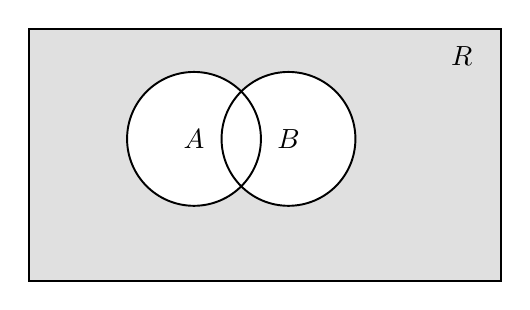
\begin{tikzpicture}[scale=1,line width=0.7pt]
\fill[black!12] (0,0) rectangle (6,3.2);
\fill[white] (2.1,1.8) circle (0.85);
\fill[white] (3.3,1.8) circle (0.85);
\draw (0,0) rectangle (6,3.2);
\draw (2.1,1.8) circle (0.85);
\draw (3.3,1.8) circle (0.85);
\node at (2.1,1.8) {$A$};
\node at (3.3,1.8) {$B$};
\node at (5.5,2.85) {$R$};
\end{tikzpicture}
\end{center}

（1）若集合 $C$ 表示图中阴影部分，用集合的运算式表示 $C$.

（2）求集合 $C$.

\ansspace*[12]

\ifanswer
\solbegin
\stepm{（1）}{由韦恩图得 $C=\overline{A\cup B}$.}
\stepm{（2）}{解 $\dfrac{x+1}{x-2}<-1$，则 $\dfrac{x+1}{x-2}+1<0$，即 $\dfrac{2x-1}{x-2}<0$，解得 $\dfrac12<x<2$，}
\step{故 $B=\left\{x\left|\dfrac12<x<2\right.\right\}$，所以 $A\cup B=\{x\mid-3\leqslant x<2\}$，}
\step{所以 $C=\overline{A\cup B}=\{x\mid x<-3\ \text{或}\ x\geqslant2\}$.}
\solend
\fi

\item 已知集合 $A=\{x\mid x^2-6x+8<0\}$，集合 $B=\{x\mid3m<x<1-m\}$.

（1）命题 $p:x\in A$，命题 $q:x\in B$，若 $p$ 是 $q$ 的充分条件，求实数 $m$ 的取值范围.

（2）若 $A\cap B=\varnothing$，求实数 $m$ 的取值范围.

\ansspace*[12]

\ifanswer
\solbegin
\stepm{（1）}{$x^2-6x+8<0\Rightarrow2<x<4\Rightarrow A=\{x\mid2<x<4\}$.}
\step{若 $p$ 是 $q$ 的充分条件，则 $A\subseteq B$，结合 $B$ 为非空集合，得 $\begin{cases}3m<1-m\\ 3m\leqslant2\\ 1-m\geqslant4\end{cases}$，}
\step{解得 $m\leqslant-3$，故 $m$ 的取值范围是 $(-\infty,-3]$；}
\stepm{（2）}{当 $B=\varnothing$ 时，$3m\geqslant1-m$，解得 $m\geqslant\dfrac14$，满足 $A\cap B=\varnothing$；}
\step{当 $B\neq\varnothing$ 时，$3m<1-m$ 即 $m<\dfrac14$，}
\step{要使交集为空，则 $1-m\leqslant2$ 或 $3m\geqslant4$，解得 $m\geqslant-1$，}
\step{结合 $m<\dfrac14$，得 $-1\leqslant m<\dfrac14$.}
\step{综上，$m\geqslant-1$，即 $m$ 的取值范围是 $[-1,+\infty)$.}
\solend
\fi

\item 设某企业每月生产电机 $x$ 台，根据企业月度报表知，每月总产值 $m$（万元）与总支出 $n$（万元）近似地满足下列关系：$m=\dfrac92x-\dfrac14$，$n=-\dfrac14x^2+5x+\dfrac74$，当 $m-n\geqslant0$ 时，称不亏损企业；当 $m-n<0$ 时，称亏损企业，且 $n-m$ 为亏损额.

（1）企业要成为不亏损企业，每月至少要生产多少台电机？

（2）当月总产值为多少时，企业亏损最严重，最大亏损额为多少？

\ansspace*[12]

\ifanswer
\solbegin
\stepm{（1）}{由题意得 $m-n\geqslant0$，即 $\dfrac92x-\dfrac14\geqslant-\dfrac14x^2+5x+\dfrac74$，}
\step{整理得 $x^2-2x-8\geqslant0$，解得 $x\geqslant4$ 或 $x\leqslant-2$（舍），}
\step{所以企业要成为不亏损企业，每月至少要生产 $4$ 台电机；}
\stepm{（2）}{由（1）得当 $0<x<4$ 时企业亏损，}
\step{亏损额 $n-m=\left(-\dfrac14x^2+5x+\dfrac74\right)-\left(\dfrac92x-\dfrac14\right)=-\dfrac14(x-1)^2+\dfrac94$，}
\step{所以当 $x=1$ 时，$n-m$ 取最大值 $\dfrac94$，}
\step{答：当月总产值为 $1$ 台时，企业亏损最严重，最大亏损额为 $\dfrac94$ 万元.}
\solend
\fi

\item 已知 $x_1$、$x_2$ 是一元二次方程 $4kx^2-4kx+k+1=0(k\neq0)$ 的两个实数根.

（1）是否存在实数 $k$，使 $x_1^2+x_2^2=\dfrac14$ 成立？若存在，求出 $k$ 的值，若不存在，请说明理由；

（2）是否存在整数 $k$，使 $\dfrac{x_1}{x_2}+\dfrac{x_2}{x_1}-2$ 的值为整数？若存在，求出 $k$ 的值，若不存在，请说明理由.

\ansspace*[14]

\ifanswer
\solbegin
\stepm{（1）}{因为 $x_1$、$x_2$ 是一元二次方程 $4kx^2-4kx+k+1=0(k\neq0)$ 的两个实数根，}
\step{所以 $\Delta=(-4k)^2-4\times4k(k+1)\geqslant0$，解得 $k\leqslant0$，}
\step{由韦达定理得 $\begin{cases}x_1+x_2=1\\ x_1x_2=\dfrac{k+1}{4k}\end{cases}$，}
\step{则 $x_1^2+x_2^2=(x_1+x_2)^2-2x_1x_2=\dfrac14$，}
\step{即 $1-2\times\dfrac{k+1}{4k}=\dfrac14$，解得 $k=2$，因为 $k\leqslant0$，所以不存在实数 $k$.}
\stepm{（2）}{$\dfrac{x_1}{x_2}+\dfrac{x_2}{x_1}-2=\dfrac{x_1^2+x_2^2}{x_1x_2}-2=\dfrac{(x_1+x_2)^2-2x_1x_2}{x_1x_2}-2=\dfrac{(x_1+x_2)^2}{x_1x_2}-4$}
\step{$=\dfrac{1}{\dfrac{k+1}{4k}}-4=\dfrac{4k}{k+1}-4=\dfrac{4k-4(k+1)}{k+1}=\dfrac{-4}{k+1}$，}
\step{由于 $\dfrac{x_1}{x_2}+\dfrac{x_2}{x_1}-2$ 的值为整数，即 $\dfrac{-4}{k+1}$ 的值为整数，}
\step{所以 $k+1$ 只能取 $\pm1$、$\pm2$、$\pm4$，}
\step{又 $k\leqslant0$，所以当 $k+1=\pm1$ 时，得出 $k=0$（舍）或 $k=-2$，}
\step{当 $k+1=\pm2$ 时，得出 $k=1$（舍）或 $k=-3$，}
\step{当 $k+1=\pm4$ 时，得出 $k=3$（舍）或 $k=-5$，}
\step{综上所述，若 $\dfrac{x_1}{x_2}+\dfrac{x_2}{x_1}-2$ 的值为整数，则 $k$ 的值为 $-2$ 或 $-3$ 或 $-5$.}
\solend
\fi

\item 已知集合 $A=\{a_1,a_2,\cdots,a_n\}(n\geqslant3)$，其中 $a_m\in\Z(m=1,2,\cdots,n)$. 若 $A$ 的子集 $T=\{a_i,a_j,a_k\}$ 满足 $2a_k=a_i+a_j$，则称 $T$ 具有性质 $P$. $A$ 的所有具有性质 $P$ 的子集 $T$ 的个数记为 $card_A(T)$.

（1）当 $A=\{4,-1,-2,1,-5\}$ 时，写出 $A$ 的所有具有性质 $P$ 的子集 $T$；

（2）当 $n=4$ 时，若 $a_1<a_2<a_3<a_4$，且 $card_A(T)=2$，证明：数对 $a_1$、$a_3$ 和 $a_2$、$a_4$ 中至少有一对中的两数奇偶性相同；

（3）当 $n=9$ 时，求 $card_A(T)$ 的最大值.

\ansspace*[14]

\ifanswer
\solbegin
\stepm{（1）}{集合 $A=\{4,-1,-2,1,-5\}$，元素按从小到大排列为 $-5$、$-2$、$-1$、$1$、$4$，}
\step{满足 $2a_k=a_i+a_j$ 的三元子集 $T$ 需满足其中一个元素是另外两个的平均数，}
\step{对于 $-5,-2,1$：$2\times(-2)=-4=-5+1$，满足条件，故 $T=\{-5,-2,1\}$，}
\step{对于 $-2,1,4$：$2\times1=2=-2+4$，满足条件，故 $T=\{-2,1,4\}$，}
\step{因此满足的子集有 $\{-5,-2,1\}$ 和 $\{-2,1,4\}$.}
\stepm{（2）}{假设数对 $(a_1,a_3)$ 和 $(a_2,a_4)$ 的两数奇偶性均不同，}
\step{即 $a_1$ 与 $a_3$ 一奇一偶，故 $a_1+a_3$ 为奇数，}
\step{$a_2$ 与 $a_4$ 一奇一偶，故 $a_2+a_4$ 为奇数，}
\step{集合 $A=\{a_1,a_2,a_3,a_4\}$ 的三元子集共 $\mathrm{C}_4^3=4$ 个：}
\step{$\{a_1,a_2,a_3\}$：若满足 $2a_2=a_1+a_3$，左边为偶数，右边为奇数，矛盾，故不满足；}
\step{$\{a_2,a_3,a_4\}$：若满足 $2a_3=a_2+a_4$，左边为偶数，右边为奇数，矛盾，故不满足；}
\step{$\{a_1,a_2,a_4\}$：需 $2a_2=a_1+a_4$；}
\step{$\{a_1,a_3,a_4\}$：需 $2a_3=a_1+a_4$.}
\step{若这两个子集都满足，则 $2a_2=2a_3\Rightarrow a_2=a_3$，与 $a_2<a_3$ 矛盾，}
\step{因此最多只有 $1$ 个子集满足条件，与 $card_A(T)=2$ 矛盾，故假设不成立，}
\step{即数对 $(a_1,a_3)$ 和 $(a_2,a_4)$ 中至少有一对的两数奇偶性相同.}
\stepm{（3）}{要最大化 $card_A(T)$，}
\step{集合 $A$ 应包含尽可能多的三元等差数列（即长度为 $3$ 的等差数列），}
\step{当 $A$ 为公差为 $1$ 的等差数列（如 $A=\{0,1,2,\cdots,8\}$）时，}
\step{三元等差数列的个数最多，}
\step{对于集合 $\{0,1,2,\cdots,8\}$，计算三元等差数列个数：}
\step{公差 $d=1$：$\{0,1,2\},\{1,2,3\},\cdots,\{6,7,8\}$，共 $7$ 个；}
\step{公差 $d=2$：$\{0,2,4\},\{1,3,5\},\cdots,\{4,6,8\}$，共 $5$ 个；}
\step{公差 $d=3$：$\{0,3,6\},\{1,4,7\},\{2,5,8\}$，共 $3$ 个；}
\step{公差 $d=4$：$\{0,4,8\}$，共 $1$ 个；}
\step{总个数为 $7+5+3+1=16$.}
\solend
\fi

\end{enumerate}

\end{document}
"
% 紧凑版：xelatex "\def\iscompact{1}% 高一89_宝山中学_10月月考.tex
%   —— 高一上数学“2026-2027 年宝山中学高一上 10 月月考”（讲评版）
% 试卷版：xelatex 高一89_宝山中学_10月月考.tex
% 答案版：xelatex "\def\isanswer{1}\input{高一89_宝山中学_10月月考.tex}"
% 紧凑版：xelatex "\def\iscompact{1}\input{高一89_宝山中学_10月月考.tex}"
%
% 原始材料：微信公众号“魔都数学加油站”文章，连载“27学年高一89”；
% 原文标题“27学年高一89——2026-2027年上海市宝山中学高一上10月月考”；
% 原文链接：https://mp.weixin.qq.com/s/DZ-Q-hfS4UulNW_vGWrZXw。
% 正文为 10 张 PNG 页（`原图/高一89_宝山中学_10月月考/01..10.png`），
% 尺寸混排（第 6 页为 2560×3620，其余为 4762×6735），均按页序读取。
%
% 篇幅与题号：原卷自第 3 题起编号（第 1、2 题不在原文内）。填空题 3—12（10 题）、
% 选择题 13—16（4 题）、解答题 17—21（5 题），共 19 题。
%
% 讲评版：第 4 题只印【答案】（“$x\leqslant2$ 或 $y\leqslant2$”），本稿只给 \ans{}；
% 其余 18 题印【解析】，其中选择题答案在解析末句“故选 C／B／A／A”。
% 第 17 题题干带一幅韦恩图（全集 $R$、集合 $A$、$B$ 与阴影部分），三版都出。
%
% 副标题：原卷未印副标题。本稿按内容标作“集合与常用逻辑用语、不等式”。
%
% 原卷笔误/存疑（均照录未改，正文对应处另有 % 注）：
%   ① 第 8 题题干“$k\in R$”与第 12 题“$n\in N$”按原卷用斜体字母排，本稿沿用
%      $\R$、$\N$ 记号（见“排版差异”③），此处不再视为笔误；
%   ② 第 9 题解析“故 $a$ 的取值范围是 $a<-1$ 或 $\dfrac13<a<\dfrac12$”，未把
%      $a<-1$ 写成区间，与同题前两行的写法不统一，属原卷写法，照录；
%   ③ 第 20 题 (1) 由 $\Delta\geqslant0$ 得“$k\leqslant0$”，与题设 $k\neq0$ 合看
%      应为 $k<0$；原卷写 $k\leqslant0$ 并以之舍去 $k=2$，结论不变，照录。
%
% 与原卷的排版差异：
%   ① 原卷每题下直接印【答案】/【解析】，本稿按全稿惯例将答案与解析置于答案版；
%   ② 原卷未印副标题，本稿补出；填空横线统一排 \blankline[4.4em]；
%   ③ 原卷数集记号排斜体 $R$、$Z$、$N$，本稿按全稿惯例改用 $\R$、$\Z$、$\N$；
%   ④ 第 17—21 题的子问用行内“（1）（2）（3）”段，解析中的子问标号用 \stepm；
%   ⑤ 解答题按惯例加 \ansspace；选择题括号排 \mbox{（\quad）}；
%   ⑥ 第 17 题的韦恩图原卷排在题干右侧、文字绕排，本稿改排为题干后的居中图
%      （TikZ 重绘：原图该处有公众号粉色水印斜压，按原图布局重绘，标注一致）。
%
% 行数核对：逐题数 \step/\stepm 条数，合计 119 条（Q3：2；Q4：0；Q5：3；Q6：4；
% Q7：2；Q8：3；Q9：4；Q10：5；Q11：8；Q12：4；Q13：5；Q14：7；Q15：9；Q16：5；
% Q17：4；Q18：8；Q19：7；Q20：13；Q21：26）。第 4 题只印【答案】，不计入 \step 账。
% 原卷解析的换行按语意合并，未逐行强拆。
%
\documentclass[a4paper,11pt]{article}
\usepackage{common}

\begin{document}

\examtitlest[7]{2026--2027 年宝山中学高一上 10 月月考}{集合与常用逻辑用语、不等式}

\bigsec{一、填空题}

\begin{enumerate}
\setcounter{enumi}{2}

\item 满足 $\{1,2\}\subseteq A\subseteq\{1,2,3,4,5\}$ 的集合共 $A$ 有\blankline[4.4em]个.

\ifanswer
\solbegin
\step{由题意得 $A=\{1,2\}$ 与 $\{3,4,5\}$ 的非空子集的并集，}
\step{而 $\{3,4,5\}$ 的子集有 $2^3=8$ 个，所以满足条件的 $A$ 有 $8$ 个.}
\solend
\fi

\item 用反证法证明命题：“若 $x+y>4$，则 $x>2$ 且 $y>2$”时，第一步应该假设\blankline[4.4em].

\ifanswer
\ans{$x\leqslant2$ 或 $y\leqslant2$}
\fi

\item 已知等式 $2x^2+3x+5=a(2x+1)(x+1)+c$ 恒成立，则 $a-c$ 的值为\blankline[4.4em].

\ifanswer
\solbegin
\step{因为 $2x^2+3x+5=a(2x+1)(x+1)+c$ 恒成立，}
\step{所以 $2x^2+3x+5=2ax^2+3ax+a+c$ 恒成立，}
\step{则 $\begin{cases}2=2a\\ 3=3a\\ 5=a+c\end{cases}$，得 $a=1$，$c=4$，所以 $a-c=-3$.}
\solend
\fi

\item 不等式 $\lvert3x-1\rvert<x$ 的解集\blankline[4.4em].

\ifanswer
\solbegin
\step{当 $x\leqslant0$ 时，不等式的解集为 $\varnothing$，}
\step{当 $x>0$ 时，$\lvert3x-1\rvert<x$，即 $(3x-1)^2<x^2$，}
\step{整理得 $8x^2-6x+1<0$，$(2x-1)(4x-1)<0$，解得 $\dfrac14<x<\dfrac12$，满足 $x>0$.}
\step{故解集为 $\left(\dfrac14,\dfrac12\right)$.}
\solend
\fi

\item 比较两个代数式的大小关系：$x^2+2y^2$\blankline[3em]$2xy+2y-1$.

\ifanswer
\solbegin
\step{$x^2+2y^2-(2xy+2y-1)=x^2-2xy+y^2+y^2-2y+1$}
\step{$=(x-y)^2+(y-1)^2\geqslant0$，所以 $x^2+2y^2\geqslant2xy+2y-1$.}
\solend
\fi

\item $k\in\R$，关于 $x$ 的不等式 $x^2+\sqrt2kx+2>0$ 的解集为全体实数，则 $k$ 的取值范围是\blankline[4.4em].

\ifanswer
\solbegin
\step{因为关于 $x$ 的不等式 $x^2+\sqrt2kx+2>0$ 的解集为全体实数，}
\step{所以 $\Delta=(\sqrt2k)^2-4\times1\times2=2k^2-8<0$，解得 $-2<k<2$，}
\step{即实数 $k$ 的取值范围是 $(-2,2)$.}
\solend
\fi

\item 在平面直角坐标系内，点 $\left(2a-1,\dfrac{3a-1}{a+1}\right)$ 在第二象限，则 $a$ 的取值范围是\blankline[4.4em].

\ifanswer
\solbegin
\step{由题意得 $\begin{cases}2a-1<0\\[0.2em]\dfrac{3a-1}{a+1}>0\end{cases}$，}
\step{由 $2a-1<0$，解得 $a<\dfrac12$；}
\step{由 $\dfrac{3a-1}{a+1}>0$，解得 $a<-1$ 或 $a>\dfrac13$；}
\step{故 $a$ 的取值范围是 $a<-1$ 或 $\dfrac13<a<\dfrac12$.}
\solend
\fi

\item 设集合 $A=\{x\mid x^2+x-6=0\}$，集合 $B=\{x\mid mx+1=0\}$，且 $A\cup B=A$，则 $m$ 的值组成的集合是\blankline[4.4em].

\ifanswer
\solbegin
\step{由题意得 $A=\{x\mid x^2+x-6=0\}=\{-3,2\}$，}
\step{由 $A\cup B=A$，得 $B\subseteq A$，}
\step{当 $m=0$ 时，$B=\varnothing$，满足题意，}
\step{当 $m\neq0$ 时，$B=\left\{-\dfrac1m\right\}$，所以 $-\dfrac1m=2$ 或 $-\dfrac1m=-3$，所以 $m=-\dfrac12$ 或 $m=\dfrac13$，}
\step{综上所述，$m$ 的值组成的集合是 $\left\{0,-\dfrac12,\dfrac13\right\}$.}
\solend
\fi

\item 甲、乙两人解关于 $x$ 的不等式 $x^2+bx+c<0$，甲写错了 $b$，正确计算后得到的解为 $\{x\mid1<x<2\}$；乙写错了 $c$，正确计算后得到的解为 $\{x\mid-4<x<1\}$. 那么不等式 $\dfrac{bx+c}{x-2}<0$ 的解为\blankline[4.4em].

\ifanswer
\solbegin
\step{由 $x^2+bx+c<0$ 的解为 $\{x\mid1<x<2\}$，}
\step{则 $1$ 和 $2$ 是方程 $x^2+bx+c=0$ 的两个根，}
\step{甲写错了 $b$，但 $c$ 是正确的，所以 $c=1\times2=2$；}
\step{由 $x^2+bx+c<0$ 的解为 $\{x\mid-4<x<1\}$，}
\step{则 $-4$ 和 $1$ 是方程 $x^2+bx+c=0$ 的两个根，}
\step{乙写错了 $c$，但 $b$ 是正确的，所以 $-b=-4+1=-3$，即 $b=3$.}
\step{由 $\dfrac{bx+c}{x-2}<0$，得 $\dfrac{3x+2}{x-2}<0$，即 $(3x+2)(x-2)<0$，解得 $-\dfrac23<x<2$，}
\step{所以不等式 $\dfrac{bx+c}{x-2}<0$ 的解为 $\left\{x\left|-\dfrac23<x<2\right.\right\}$.}
\solend
\fi

\item 已知集合 $M$ 的元素均为正整数，定义集合 $M$ 的“变项和”为：将 $M$ 中每个元素 $m$ 都乘以 $(-1)^m$ 后再求和. 若集合 $A=\{n\mid1\leqslant n\leqslant10,n\in\N\}$，则集合 $A$ 的所有非空子集的“变项和”的总和为\blankline[4.4em].

\ifanswer
\solbegin
\step{$A$ 集合的所有非空子集中，每个元素出现的次数都是 $(2^{10}-1)-(2^9-1)=2^9$，}
\step{则集合 $A$ 的所有非空子集的“变项和”的总和}
\step{为 $1\times(-1)^1\times2^9+2\times(-1)^2\times2^9+\cdots+10\times(-1)^{10}\times2^9$}
\step{$=(-1+2-3+4-\cdots-9+10)\times2^9=5\times2^9=2560$.}
\solend
\fi

\end{enumerate}

\bigsec{二、选择题}

\begin{enumerate}
\setcounter{enumi}{12}

\item 下列命题中正确的是\mbox{（\quad）}

\keepwithprev
A. 若 $a>b$，则 $\dfrac1a<\dfrac1b$\qquad B. 若 $a>b$，则 $a^2>b^2$

C. 若 $a>\lvert b\rvert$，则 $a>b$\qquad D. 若 $a>b$，则 $ac^2>bc^2$

\ifanswer
\solbegin
\step{对于 $AB$ 选项，取 $a=1$，$b=-1$，$a>b$，$\dfrac1a>\dfrac1b$，$a^2=b^2$，}
\step{所以 $AB$ 选项错误；}
\step{对于 $C$ 选项，由 $a>\lvert b\rvert$，$\lvert b\rvert\geqslant b$，得 $a>b$，所以 $C$ 选项正确；}
\step{对于 $D$ 选项，取 $c=0$，则 $ac^2=0=bc^2$，所以 $D$ 选项错误.}
\step{故选 $C$.}
\solend
\fi

\item 下面关于集合的表示正确的个数是\mbox{（\quad）}

①$\{1,2,3\}=\{3,2,1\}$；\quad ②$\{(x,y)\mid x-y=1\}=\{y\mid y=x-1\}$；

③$\{x\mid x\geqslant2,x\in\N\}=\{y\mid y\geqslant2,y\in\Z\}$；\quad ④$\{x\mid x+2y=1\}\neq\left\{y\left|y=-\dfrac12x+\dfrac12\right.\right\}$.

\keepwithprev
A. $1$\qquad B. $2$\qquad C. $3$\qquad D. $4$

\ifanswer
\solbegin
\step{对于①，由元素的无序性得①正确；}
\step{对于②，$\{(x,y)\mid x-y=1\}$ 表示点集，$\{y\mid y=x-1\}$ 表示数集，故②错误；}
\step{对于③，$\{x\mid x\geqslant2,x\in\N\}$ 表示大于等于 $2$ 的整数，}
\step{$\{y\mid y\geqslant2,y\in\Z\}$ 也表示大于等于 $2$ 的整数，故③正确；}
\step{对于④，$\{x\mid x+2y=1\}=\R$，$\left\{y\left|y=-\dfrac12x+\dfrac12\right.\right\}=\R$，}
\step{所以 $\{x\mid x+2y=1\}=\left\{y\left|y=-\dfrac12x+\dfrac12\right.\right\}$，故④错误，}
\step{所以正确的个数是 $2$ 个. 故选 $B$.}
\solend
\fi

\item 已知命题 $P$：方程 $ax^2+bx+c=0$ 有两个不相等实根；命题 $Q$：不等式 $ax^2+bx+c>0$ 与 $ax^2+bx+c<0$ 均有解，则命题 $P$ 成立是命题 $Q$ 成立的\mbox{（\quad）}条件.

\keepwithprev
A. 充分非必要条件\qquad B. 必要非充分条件

C. 充要条件\qquad D. 既非充分又非必要条件

\ifanswer
\solbegin
\step{若 $P$ 成立，即方程 $ax^2+bx+c=0$ 有两个不相等实根，}
\step{此时 $\begin{cases}a\neq0\\ \Delta=b^2-4ac>0\end{cases}$；}
\step{若 $Q$ 成立，即不等式 $ax^2+bx+c>0$ 与 $ax^2+bx+c<0$ 均有解，有两种情况：}
\step{①不等式是一元二次不等式，}
\step{此时不等式所对应的二次函数的图像与 $x$ 轴有两个交点，}
\step{满足 $\begin{cases}a\neq0\\ \Delta=b^2-4ac>0\end{cases}$；}
\step{②不等式是一元一次不等式，此时 $\begin{cases}a=0\\ b\neq0\end{cases}$，}
\step{因此，由 $P$ 能推出 $Q$ 成立，但是由 $Q$ 不能推出 $P$ 成立，}
\step{即 $P$ 是 $Q$ 的充分非必要条件. 故选 $A$.}
\solend
\fi

\item 甲、乙同去加油站加油两次，两次汽油单价分别为 $x$、$y$ 元/升（$x\neq y$）. 甲每次加固定金额的油，乙每次加固定体积的油. 哪种方式更经济实惠呢？\mbox{（\quad）}

\keepwithprev
A. 加固定金额的方式\qquad B. 加固定体积的方式

C. 两种方案一样\qquad D. 要视具体价格而定

\ifanswer
\solbegin
\step{设两次加油的油价分别为 $x$、$y$（$x$、$y>0$，且 $x\neq y$），}
\step{乙每次加油的量为 $a$（$a>0$）；甲每次加油的钱数为 $b$（$b>0$），}
\step{则乙平均油价为 $\dfrac{ax+ay}{2a}=\dfrac{x+y}{2}$，甲平均油价为 $\dfrac{2b}{\dfrac bx+\dfrac by}=\dfrac2{\dfrac1x+\dfrac1y}=\dfrac{2xy}{x+y}$，}
\step{因为 $x\neq y$，所以 $\dfrac{x+y}{2}-\dfrac{2xy}{x+y}=\dfrac{(x-y)^2}{2(x+y)}>0$，所以 $\dfrac{x+y}{2}>\dfrac{2xy}{x+y}$，}
\step{即甲方案更经济. 故选 $A$.}
\solend
\fi

\end{enumerate}

\bigsec{三、解答题}

\begin{enumerate}
\setcounter{enumi}{16}

\item 已知全集 $U=\R$，集合 $A=\{x\mid-3\leqslant x\leqslant1\}$，$B=\left\{x\left|\dfrac{x+1}{x-2}<-1\right.\right\}$.

\begin{center}
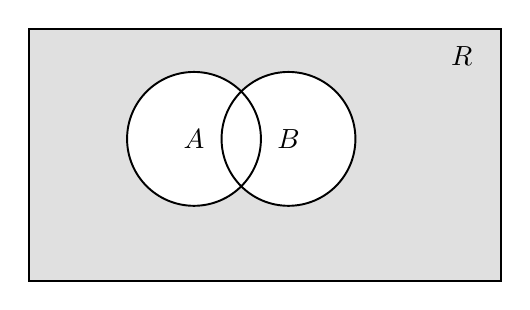
\begin{tikzpicture}[scale=1,line width=0.7pt]
\fill[black!12] (0,0) rectangle (6,3.2);
\fill[white] (2.1,1.8) circle (0.85);
\fill[white] (3.3,1.8) circle (0.85);
\draw (0,0) rectangle (6,3.2);
\draw (2.1,1.8) circle (0.85);
\draw (3.3,1.8) circle (0.85);
\node at (2.1,1.8) {$A$};
\node at (3.3,1.8) {$B$};
\node at (5.5,2.85) {$R$};
\end{tikzpicture}
\end{center}

（1）若集合 $C$ 表示图中阴影部分，用集合的运算式表示 $C$.

（2）求集合 $C$.

\ansspace*[12]

\ifanswer
\solbegin
\stepm{（1）}{由韦恩图得 $C=\overline{A\cup B}$.}
\stepm{（2）}{解 $\dfrac{x+1}{x-2}<-1$，则 $\dfrac{x+1}{x-2}+1<0$，即 $\dfrac{2x-1}{x-2}<0$，解得 $\dfrac12<x<2$，}
\step{故 $B=\left\{x\left|\dfrac12<x<2\right.\right\}$，所以 $A\cup B=\{x\mid-3\leqslant x<2\}$，}
\step{所以 $C=\overline{A\cup B}=\{x\mid x<-3\ \text{或}\ x\geqslant2\}$.}
\solend
\fi

\item 已知集合 $A=\{x\mid x^2-6x+8<0\}$，集合 $B=\{x\mid3m<x<1-m\}$.

（1）命题 $p:x\in A$，命题 $q:x\in B$，若 $p$ 是 $q$ 的充分条件，求实数 $m$ 的取值范围.

（2）若 $A\cap B=\varnothing$，求实数 $m$ 的取值范围.

\ansspace*[12]

\ifanswer
\solbegin
\stepm{（1）}{$x^2-6x+8<0\Rightarrow2<x<4\Rightarrow A=\{x\mid2<x<4\}$.}
\step{若 $p$ 是 $q$ 的充分条件，则 $A\subseteq B$，结合 $B$ 为非空集合，得 $\begin{cases}3m<1-m\\ 3m\leqslant2\\ 1-m\geqslant4\end{cases}$，}
\step{解得 $m\leqslant-3$，故 $m$ 的取值范围是 $(-\infty,-3]$；}
\stepm{（2）}{当 $B=\varnothing$ 时，$3m\geqslant1-m$，解得 $m\geqslant\dfrac14$，满足 $A\cap B=\varnothing$；}
\step{当 $B\neq\varnothing$ 时，$3m<1-m$ 即 $m<\dfrac14$，}
\step{要使交集为空，则 $1-m\leqslant2$ 或 $3m\geqslant4$，解得 $m\geqslant-1$，}
\step{结合 $m<\dfrac14$，得 $-1\leqslant m<\dfrac14$.}
\step{综上，$m\geqslant-1$，即 $m$ 的取值范围是 $[-1,+\infty)$.}
\solend
\fi

\item 设某企业每月生产电机 $x$ 台，根据企业月度报表知，每月总产值 $m$（万元）与总支出 $n$（万元）近似地满足下列关系：$m=\dfrac92x-\dfrac14$，$n=-\dfrac14x^2+5x+\dfrac74$，当 $m-n\geqslant0$ 时，称不亏损企业；当 $m-n<0$ 时，称亏损企业，且 $n-m$ 为亏损额.

（1）企业要成为不亏损企业，每月至少要生产多少台电机？

（2）当月总产值为多少时，企业亏损最严重，最大亏损额为多少？

\ansspace*[12]

\ifanswer
\solbegin
\stepm{（1）}{由题意得 $m-n\geqslant0$，即 $\dfrac92x-\dfrac14\geqslant-\dfrac14x^2+5x+\dfrac74$，}
\step{整理得 $x^2-2x-8\geqslant0$，解得 $x\geqslant4$ 或 $x\leqslant-2$（舍），}
\step{所以企业要成为不亏损企业，每月至少要生产 $4$ 台电机；}
\stepm{（2）}{由（1）得当 $0<x<4$ 时企业亏损，}
\step{亏损额 $n-m=\left(-\dfrac14x^2+5x+\dfrac74\right)-\left(\dfrac92x-\dfrac14\right)=-\dfrac14(x-1)^2+\dfrac94$，}
\step{所以当 $x=1$ 时，$n-m$ 取最大值 $\dfrac94$，}
\step{答：当月总产值为 $1$ 台时，企业亏损最严重，最大亏损额为 $\dfrac94$ 万元.}
\solend
\fi

\item 已知 $x_1$、$x_2$ 是一元二次方程 $4kx^2-4kx+k+1=0(k\neq0)$ 的两个实数根.

（1）是否存在实数 $k$，使 $x_1^2+x_2^2=\dfrac14$ 成立？若存在，求出 $k$ 的值，若不存在，请说明理由；

（2）是否存在整数 $k$，使 $\dfrac{x_1}{x_2}+\dfrac{x_2}{x_1}-2$ 的值为整数？若存在，求出 $k$ 的值，若不存在，请说明理由.

\ansspace*[14]

\ifanswer
\solbegin
\stepm{（1）}{因为 $x_1$、$x_2$ 是一元二次方程 $4kx^2-4kx+k+1=0(k\neq0)$ 的两个实数根，}
\step{所以 $\Delta=(-4k)^2-4\times4k(k+1)\geqslant0$，解得 $k\leqslant0$，}
\step{由韦达定理得 $\begin{cases}x_1+x_2=1\\ x_1x_2=\dfrac{k+1}{4k}\end{cases}$，}
\step{则 $x_1^2+x_2^2=(x_1+x_2)^2-2x_1x_2=\dfrac14$，}
\step{即 $1-2\times\dfrac{k+1}{4k}=\dfrac14$，解得 $k=2$，因为 $k\leqslant0$，所以不存在实数 $k$.}
\stepm{（2）}{$\dfrac{x_1}{x_2}+\dfrac{x_2}{x_1}-2=\dfrac{x_1^2+x_2^2}{x_1x_2}-2=\dfrac{(x_1+x_2)^2-2x_1x_2}{x_1x_2}-2=\dfrac{(x_1+x_2)^2}{x_1x_2}-4$}
\step{$=\dfrac{1}{\dfrac{k+1}{4k}}-4=\dfrac{4k}{k+1}-4=\dfrac{4k-4(k+1)}{k+1}=\dfrac{-4}{k+1}$，}
\step{由于 $\dfrac{x_1}{x_2}+\dfrac{x_2}{x_1}-2$ 的值为整数，即 $\dfrac{-4}{k+1}$ 的值为整数，}
\step{所以 $k+1$ 只能取 $\pm1$、$\pm2$、$\pm4$，}
\step{又 $k\leqslant0$，所以当 $k+1=\pm1$ 时，得出 $k=0$（舍）或 $k=-2$，}
\step{当 $k+1=\pm2$ 时，得出 $k=1$（舍）或 $k=-3$，}
\step{当 $k+1=\pm4$ 时，得出 $k=3$（舍）或 $k=-5$，}
\step{综上所述，若 $\dfrac{x_1}{x_2}+\dfrac{x_2}{x_1}-2$ 的值为整数，则 $k$ 的值为 $-2$ 或 $-3$ 或 $-5$.}
\solend
\fi

\item 已知集合 $A=\{a_1,a_2,\cdots,a_n\}(n\geqslant3)$，其中 $a_m\in\Z(m=1,2,\cdots,n)$. 若 $A$ 的子集 $T=\{a_i,a_j,a_k\}$ 满足 $2a_k=a_i+a_j$，则称 $T$ 具有性质 $P$. $A$ 的所有具有性质 $P$ 的子集 $T$ 的个数记为 $card_A(T)$.

（1）当 $A=\{4,-1,-2,1,-5\}$ 时，写出 $A$ 的所有具有性质 $P$ 的子集 $T$；

（2）当 $n=4$ 时，若 $a_1<a_2<a_3<a_4$，且 $card_A(T)=2$，证明：数对 $a_1$、$a_3$ 和 $a_2$、$a_4$ 中至少有一对中的两数奇偶性相同；

（3）当 $n=9$ 时，求 $card_A(T)$ 的最大值.

\ansspace*[14]

\ifanswer
\solbegin
\stepm{（1）}{集合 $A=\{4,-1,-2,1,-5\}$，元素按从小到大排列为 $-5$、$-2$、$-1$、$1$、$4$，}
\step{满足 $2a_k=a_i+a_j$ 的三元子集 $T$ 需满足其中一个元素是另外两个的平均数，}
\step{对于 $-5,-2,1$：$2\times(-2)=-4=-5+1$，满足条件，故 $T=\{-5,-2,1\}$，}
\step{对于 $-2,1,4$：$2\times1=2=-2+4$，满足条件，故 $T=\{-2,1,4\}$，}
\step{因此满足的子集有 $\{-5,-2,1\}$ 和 $\{-2,1,4\}$.}
\stepm{（2）}{假设数对 $(a_1,a_3)$ 和 $(a_2,a_4)$ 的两数奇偶性均不同，}
\step{即 $a_1$ 与 $a_3$ 一奇一偶，故 $a_1+a_3$ 为奇数，}
\step{$a_2$ 与 $a_4$ 一奇一偶，故 $a_2+a_4$ 为奇数，}
\step{集合 $A=\{a_1,a_2,a_3,a_4\}$ 的三元子集共 $\mathrm{C}_4^3=4$ 个：}
\step{$\{a_1,a_2,a_3\}$：若满足 $2a_2=a_1+a_3$，左边为偶数，右边为奇数，矛盾，故不满足；}
\step{$\{a_2,a_3,a_4\}$：若满足 $2a_3=a_2+a_4$，左边为偶数，右边为奇数，矛盾，故不满足；}
\step{$\{a_1,a_2,a_4\}$：需 $2a_2=a_1+a_4$；}
\step{$\{a_1,a_3,a_4\}$：需 $2a_3=a_1+a_4$.}
\step{若这两个子集都满足，则 $2a_2=2a_3\Rightarrow a_2=a_3$，与 $a_2<a_3$ 矛盾，}
\step{因此最多只有 $1$ 个子集满足条件，与 $card_A(T)=2$ 矛盾，故假设不成立，}
\step{即数对 $(a_1,a_3)$ 和 $(a_2,a_4)$ 中至少有一对的两数奇偶性相同.}
\stepm{（3）}{要最大化 $card_A(T)$，}
\step{集合 $A$ 应包含尽可能多的三元等差数列（即长度为 $3$ 的等差数列），}
\step{当 $A$ 为公差为 $1$ 的等差数列（如 $A=\{0,1,2,\cdots,8\}$）时，}
\step{三元等差数列的个数最多，}
\step{对于集合 $\{0,1,2,\cdots,8\}$，计算三元等差数列个数：}
\step{公差 $d=1$：$\{0,1,2\},\{1,2,3\},\cdots,\{6,7,8\}$，共 $7$ 个；}
\step{公差 $d=2$：$\{0,2,4\},\{1,3,5\},\cdots,\{4,6,8\}$，共 $5$ 个；}
\step{公差 $d=3$：$\{0,3,6\},\{1,4,7\},\{2,5,8\}$，共 $3$ 个；}
\step{公差 $d=4$：$\{0,4,8\}$，共 $1$ 个；}
\step{总个数为 $7+5+3+1=16$.}
\solend
\fi

\end{enumerate}

\end{document}
"
%
% 原始材料：微信公众号“魔都数学加油站”文章，连载“27学年高一89”；
% 原文标题“27学年高一89——2026-2027年上海市宝山中学高一上10月月考”；
% 原文链接：https://mp.weixin.qq.com/s/DZ-Q-hfS4UulNW_vGWrZXw。
% 正文为 10 张 PNG 页（`原图/高一89_宝山中学_10月月考/01..10.png`），
% 尺寸混排（第 6 页为 2560×3620，其余为 4762×6735），均按页序读取。
%
% 篇幅与题号：原卷自第 3 题起编号（第 1、2 题不在原文内）。填空题 3—12（10 题）、
% 选择题 13—16（4 题）、解答题 17—21（5 题），共 19 题。
%
% 讲评版：第 4 题只印【答案】（“$x\leqslant2$ 或 $y\leqslant2$”），本稿只给 \ans{}；
% 其余 18 题印【解析】，其中选择题答案在解析末句“故选 C／B／A／A”。
% 第 17 题题干带一幅韦恩图（全集 $R$、集合 $A$、$B$ 与阴影部分），三版都出。
%
% 副标题：原卷未印副标题。本稿按内容标作“集合与常用逻辑用语、不等式”。
%
% 原卷笔误/存疑（均照录未改，正文对应处另有 % 注）：
%   ① 第 8 题题干“$k\in R$”与第 12 题“$n\in N$”按原卷用斜体字母排，本稿沿用
%      $\R$、$\N$ 记号（见“排版差异”③），此处不再视为笔误；
%   ② 第 9 题解析“故 $a$ 的取值范围是 $a<-1$ 或 $\dfrac13<a<\dfrac12$”，未把
%      $a<-1$ 写成区间，与同题前两行的写法不统一，属原卷写法，照录；
%   ③ 第 20 题 (1) 由 $\Delta\geqslant0$ 得“$k\leqslant0$”，与题设 $k\neq0$ 合看
%      应为 $k<0$；原卷写 $k\leqslant0$ 并以之舍去 $k=2$，结论不变，照录。
%
% 与原卷的排版差异：
%   ① 原卷每题下直接印【答案】/【解析】，本稿按全稿惯例将答案与解析置于答案版；
%   ② 原卷未印副标题，本稿补出；填空横线统一排 \blankline[4.4em]；
%   ③ 原卷数集记号排斜体 $R$、$Z$、$N$，本稿按全稿惯例改用 $\R$、$\Z$、$\N$；
%   ④ 第 17—21 题的子问用行内“（1）（2）（3）”段，解析中的子问标号用 \stepm；
%   ⑤ 解答题按惯例加 \ansspace；选择题括号排 \mbox{（\quad）}；
%   ⑥ 第 17 题的韦恩图原卷排在题干右侧、文字绕排，本稿改排为题干后的居中图
%      （TikZ 重绘：原图该处有公众号粉色水印斜压，按原图布局重绘，标注一致）。
%
% 行数核对：逐题数 \step/\stepm 条数，合计 119 条（Q3：2；Q4：0；Q5：3；Q6：4；
% Q7：2；Q8：3；Q9：4；Q10：5；Q11：8；Q12：4；Q13：5；Q14：7；Q15：9；Q16：5；
% Q17：4；Q18：8；Q19：7；Q20：13；Q21：26）。第 4 题只印【答案】，不计入 \step 账。
% 原卷解析的换行按语意合并，未逐行强拆。
%
\documentclass[a4paper,11pt]{article}
\usepackage{common}

\begin{document}

\examtitlest[7]{2026--2027 年宝山中学高一上 10 月月考}{集合与常用逻辑用语、不等式}

\bigsec{一、填空题}

\begin{enumerate}
\setcounter{enumi}{2}

\item 满足 $\{1,2\}\subseteq A\subseteq\{1,2,3,4,5\}$ 的集合共 $A$ 有\blankline[4.4em]个.

\ifanswer
\solbegin
\step{由题意得 $A=\{1,2\}$ 与 $\{3,4,5\}$ 的非空子集的并集，}
\step{而 $\{3,4,5\}$ 的子集有 $2^3=8$ 个，所以满足条件的 $A$ 有 $8$ 个.}
\solend
\fi

\item 用反证法证明命题：“若 $x+y>4$，则 $x>2$ 且 $y>2$”时，第一步应该假设\blankline[4.4em].

\ifanswer
\ans{$x\leqslant2$ 或 $y\leqslant2$}
\fi

\item 已知等式 $2x^2+3x+5=a(2x+1)(x+1)+c$ 恒成立，则 $a-c$ 的值为\blankline[4.4em].

\ifanswer
\solbegin
\step{因为 $2x^2+3x+5=a(2x+1)(x+1)+c$ 恒成立，}
\step{所以 $2x^2+3x+5=2ax^2+3ax+a+c$ 恒成立，}
\step{则 $\begin{cases}2=2a\\ 3=3a\\ 5=a+c\end{cases}$，得 $a=1$，$c=4$，所以 $a-c=-3$.}
\solend
\fi

\item 不等式 $\lvert3x-1\rvert<x$ 的解集\blankline[4.4em].

\ifanswer
\solbegin
\step{当 $x\leqslant0$ 时，不等式的解集为 $\varnothing$，}
\step{当 $x>0$ 时，$\lvert3x-1\rvert<x$，即 $(3x-1)^2<x^2$，}
\step{整理得 $8x^2-6x+1<0$，$(2x-1)(4x-1)<0$，解得 $\dfrac14<x<\dfrac12$，满足 $x>0$.}
\step{故解集为 $\left(\dfrac14,\dfrac12\right)$.}
\solend
\fi

\item 比较两个代数式的大小关系：$x^2+2y^2$\blankline[3em]$2xy+2y-1$.

\ifanswer
\solbegin
\step{$x^2+2y^2-(2xy+2y-1)=x^2-2xy+y^2+y^2-2y+1$}
\step{$=(x-y)^2+(y-1)^2\geqslant0$，所以 $x^2+2y^2\geqslant2xy+2y-1$.}
\solend
\fi

\item $k\in\R$，关于 $x$ 的不等式 $x^2+\sqrt2kx+2>0$ 的解集为全体实数，则 $k$ 的取值范围是\blankline[4.4em].

\ifanswer
\solbegin
\step{因为关于 $x$ 的不等式 $x^2+\sqrt2kx+2>0$ 的解集为全体实数，}
\step{所以 $\Delta=(\sqrt2k)^2-4\times1\times2=2k^2-8<0$，解得 $-2<k<2$，}
\step{即实数 $k$ 的取值范围是 $(-2,2)$.}
\solend
\fi

\item 在平面直角坐标系内，点 $\left(2a-1,\dfrac{3a-1}{a+1}\right)$ 在第二象限，则 $a$ 的取值范围是\blankline[4.4em].

\ifanswer
\solbegin
\step{由题意得 $\begin{cases}2a-1<0\\[0.2em]\dfrac{3a-1}{a+1}>0\end{cases}$，}
\step{由 $2a-1<0$，解得 $a<\dfrac12$；}
\step{由 $\dfrac{3a-1}{a+1}>0$，解得 $a<-1$ 或 $a>\dfrac13$；}
\step{故 $a$ 的取值范围是 $a<-1$ 或 $\dfrac13<a<\dfrac12$.}
\solend
\fi

\item 设集合 $A=\{x\mid x^2+x-6=0\}$，集合 $B=\{x\mid mx+1=0\}$，且 $A\cup B=A$，则 $m$ 的值组成的集合是\blankline[4.4em].

\ifanswer
\solbegin
\step{由题意得 $A=\{x\mid x^2+x-6=0\}=\{-3,2\}$，}
\step{由 $A\cup B=A$，得 $B\subseteq A$，}
\step{当 $m=0$ 时，$B=\varnothing$，满足题意，}
\step{当 $m\neq0$ 时，$B=\left\{-\dfrac1m\right\}$，所以 $-\dfrac1m=2$ 或 $-\dfrac1m=-3$，所以 $m=-\dfrac12$ 或 $m=\dfrac13$，}
\step{综上所述，$m$ 的值组成的集合是 $\left\{0,-\dfrac12,\dfrac13\right\}$.}
\solend
\fi

\item 甲、乙两人解关于 $x$ 的不等式 $x^2+bx+c<0$，甲写错了 $b$，正确计算后得到的解为 $\{x\mid1<x<2\}$；乙写错了 $c$，正确计算后得到的解为 $\{x\mid-4<x<1\}$. 那么不等式 $\dfrac{bx+c}{x-2}<0$ 的解为\blankline[4.4em].

\ifanswer
\solbegin
\step{由 $x^2+bx+c<0$ 的解为 $\{x\mid1<x<2\}$，}
\step{则 $1$ 和 $2$ 是方程 $x^2+bx+c=0$ 的两个根，}
\step{甲写错了 $b$，但 $c$ 是正确的，所以 $c=1\times2=2$；}
\step{由 $x^2+bx+c<0$ 的解为 $\{x\mid-4<x<1\}$，}
\step{则 $-4$ 和 $1$ 是方程 $x^2+bx+c=0$ 的两个根，}
\step{乙写错了 $c$，但 $b$ 是正确的，所以 $-b=-4+1=-3$，即 $b=3$.}
\step{由 $\dfrac{bx+c}{x-2}<0$，得 $\dfrac{3x+2}{x-2}<0$，即 $(3x+2)(x-2)<0$，解得 $-\dfrac23<x<2$，}
\step{所以不等式 $\dfrac{bx+c}{x-2}<0$ 的解为 $\left\{x\left|-\dfrac23<x<2\right.\right\}$.}
\solend
\fi

\item 已知集合 $M$ 的元素均为正整数，定义集合 $M$ 的“变项和”为：将 $M$ 中每个元素 $m$ 都乘以 $(-1)^m$ 后再求和. 若集合 $A=\{n\mid1\leqslant n\leqslant10,n\in\N\}$，则集合 $A$ 的所有非空子集的“变项和”的总和为\blankline[4.4em].

\ifanswer
\solbegin
\step{$A$ 集合的所有非空子集中，每个元素出现的次数都是 $(2^{10}-1)-(2^9-1)=2^9$，}
\step{则集合 $A$ 的所有非空子集的“变项和”的总和}
\step{为 $1\times(-1)^1\times2^9+2\times(-1)^2\times2^9+\cdots+10\times(-1)^{10}\times2^9$}
\step{$=(-1+2-3+4-\cdots-9+10)\times2^9=5\times2^9=2560$.}
\solend
\fi

\end{enumerate}

\bigsec{二、选择题}

\begin{enumerate}
\setcounter{enumi}{12}

\item 下列命题中正确的是\mbox{（\quad）}

\keepwithprev
A. 若 $a>b$，则 $\dfrac1a<\dfrac1b$\qquad B. 若 $a>b$，则 $a^2>b^2$

C. 若 $a>\lvert b\rvert$，则 $a>b$\qquad D. 若 $a>b$，则 $ac^2>bc^2$

\ifanswer
\solbegin
\step{对于 $AB$ 选项，取 $a=1$，$b=-1$，$a>b$，$\dfrac1a>\dfrac1b$，$a^2=b^2$，}
\step{所以 $AB$ 选项错误；}
\step{对于 $C$ 选项，由 $a>\lvert b\rvert$，$\lvert b\rvert\geqslant b$，得 $a>b$，所以 $C$ 选项正确；}
\step{对于 $D$ 选项，取 $c=0$，则 $ac^2=0=bc^2$，所以 $D$ 选项错误.}
\step{故选 $C$.}
\solend
\fi

\item 下面关于集合的表示正确的个数是\mbox{（\quad）}

①$\{1,2,3\}=\{3,2,1\}$；\quad ②$\{(x,y)\mid x-y=1\}=\{y\mid y=x-1\}$；

③$\{x\mid x\geqslant2,x\in\N\}=\{y\mid y\geqslant2,y\in\Z\}$；\quad ④$\{x\mid x+2y=1\}\neq\left\{y\left|y=-\dfrac12x+\dfrac12\right.\right\}$.

\keepwithprev
A. $1$\qquad B. $2$\qquad C. $3$\qquad D. $4$

\ifanswer
\solbegin
\step{对于①，由元素的无序性得①正确；}
\step{对于②，$\{(x,y)\mid x-y=1\}$ 表示点集，$\{y\mid y=x-1\}$ 表示数集，故②错误；}
\step{对于③，$\{x\mid x\geqslant2,x\in\N\}$ 表示大于等于 $2$ 的整数，}
\step{$\{y\mid y\geqslant2,y\in\Z\}$ 也表示大于等于 $2$ 的整数，故③正确；}
\step{对于④，$\{x\mid x+2y=1\}=\R$，$\left\{y\left|y=-\dfrac12x+\dfrac12\right.\right\}=\R$，}
\step{所以 $\{x\mid x+2y=1\}=\left\{y\left|y=-\dfrac12x+\dfrac12\right.\right\}$，故④错误，}
\step{所以正确的个数是 $2$ 个. 故选 $B$.}
\solend
\fi

\item 已知命题 $P$：方程 $ax^2+bx+c=0$ 有两个不相等实根；命题 $Q$：不等式 $ax^2+bx+c>0$ 与 $ax^2+bx+c<0$ 均有解，则命题 $P$ 成立是命题 $Q$ 成立的\mbox{（\quad）}条件.

\keepwithprev
A. 充分非必要条件\qquad B. 必要非充分条件

C. 充要条件\qquad D. 既非充分又非必要条件

\ifanswer
\solbegin
\step{若 $P$ 成立，即方程 $ax^2+bx+c=0$ 有两个不相等实根，}
\step{此时 $\begin{cases}a\neq0\\ \Delta=b^2-4ac>0\end{cases}$；}
\step{若 $Q$ 成立，即不等式 $ax^2+bx+c>0$ 与 $ax^2+bx+c<0$ 均有解，有两种情况：}
\step{①不等式是一元二次不等式，}
\step{此时不等式所对应的二次函数的图像与 $x$ 轴有两个交点，}
\step{满足 $\begin{cases}a\neq0\\ \Delta=b^2-4ac>0\end{cases}$；}
\step{②不等式是一元一次不等式，此时 $\begin{cases}a=0\\ b\neq0\end{cases}$，}
\step{因此，由 $P$ 能推出 $Q$ 成立，但是由 $Q$ 不能推出 $P$ 成立，}
\step{即 $P$ 是 $Q$ 的充分非必要条件. 故选 $A$.}
\solend
\fi

\item 甲、乙同去加油站加油两次，两次汽油单价分别为 $x$、$y$ 元/升（$x\neq y$）. 甲每次加固定金额的油，乙每次加固定体积的油. 哪种方式更经济实惠呢？\mbox{（\quad）}

\keepwithprev
A. 加固定金额的方式\qquad B. 加固定体积的方式

C. 两种方案一样\qquad D. 要视具体价格而定

\ifanswer
\solbegin
\step{设两次加油的油价分别为 $x$、$y$（$x$、$y>0$，且 $x\neq y$），}
\step{乙每次加油的量为 $a$（$a>0$）；甲每次加油的钱数为 $b$（$b>0$），}
\step{则乙平均油价为 $\dfrac{ax+ay}{2a}=\dfrac{x+y}{2}$，甲平均油价为 $\dfrac{2b}{\dfrac bx+\dfrac by}=\dfrac2{\dfrac1x+\dfrac1y}=\dfrac{2xy}{x+y}$，}
\step{因为 $x\neq y$，所以 $\dfrac{x+y}{2}-\dfrac{2xy}{x+y}=\dfrac{(x-y)^2}{2(x+y)}>0$，所以 $\dfrac{x+y}{2}>\dfrac{2xy}{x+y}$，}
\step{即甲方案更经济. 故选 $A$.}
\solend
\fi

\end{enumerate}

\bigsec{三、解答题}

\begin{enumerate}
\setcounter{enumi}{16}

\item 已知全集 $U=\R$，集合 $A=\{x\mid-3\leqslant x\leqslant1\}$，$B=\left\{x\left|\dfrac{x+1}{x-2}<-1\right.\right\}$.

\begin{center}
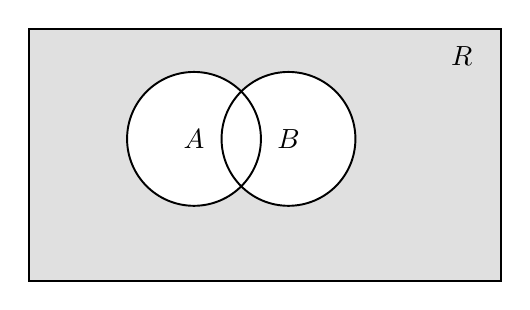
\begin{tikzpicture}[scale=1,line width=0.7pt]
\fill[black!12] (0,0) rectangle (6,3.2);
\fill[white] (2.1,1.8) circle (0.85);
\fill[white] (3.3,1.8) circle (0.85);
\draw (0,0) rectangle (6,3.2);
\draw (2.1,1.8) circle (0.85);
\draw (3.3,1.8) circle (0.85);
\node at (2.1,1.8) {$A$};
\node at (3.3,1.8) {$B$};
\node at (5.5,2.85) {$R$};
\end{tikzpicture}
\end{center}

（1）若集合 $C$ 表示图中阴影部分，用集合的运算式表示 $C$.

（2）求集合 $C$.

\ansspace*[12]

\ifanswer
\solbegin
\stepm{（1）}{由韦恩图得 $C=\overline{A\cup B}$.}
\stepm{（2）}{解 $\dfrac{x+1}{x-2}<-1$，则 $\dfrac{x+1}{x-2}+1<0$，即 $\dfrac{2x-1}{x-2}<0$，解得 $\dfrac12<x<2$，}
\step{故 $B=\left\{x\left|\dfrac12<x<2\right.\right\}$，所以 $A\cup B=\{x\mid-3\leqslant x<2\}$，}
\step{所以 $C=\overline{A\cup B}=\{x\mid x<-3\ \text{或}\ x\geqslant2\}$.}
\solend
\fi

\item 已知集合 $A=\{x\mid x^2-6x+8<0\}$，集合 $B=\{x\mid3m<x<1-m\}$.

（1）命题 $p:x\in A$，命题 $q:x\in B$，若 $p$ 是 $q$ 的充分条件，求实数 $m$ 的取值范围.

（2）若 $A\cap B=\varnothing$，求实数 $m$ 的取值范围.

\ansspace*[12]

\ifanswer
\solbegin
\stepm{（1）}{$x^2-6x+8<0\Rightarrow2<x<4\Rightarrow A=\{x\mid2<x<4\}$.}
\step{若 $p$ 是 $q$ 的充分条件，则 $A\subseteq B$，结合 $B$ 为非空集合，得 $\begin{cases}3m<1-m\\ 3m\leqslant2\\ 1-m\geqslant4\end{cases}$，}
\step{解得 $m\leqslant-3$，故 $m$ 的取值范围是 $(-\infty,-3]$；}
\stepm{（2）}{当 $B=\varnothing$ 时，$3m\geqslant1-m$，解得 $m\geqslant\dfrac14$，满足 $A\cap B=\varnothing$；}
\step{当 $B\neq\varnothing$ 时，$3m<1-m$ 即 $m<\dfrac14$，}
\step{要使交集为空，则 $1-m\leqslant2$ 或 $3m\geqslant4$，解得 $m\geqslant-1$，}
\step{结合 $m<\dfrac14$，得 $-1\leqslant m<\dfrac14$.}
\step{综上，$m\geqslant-1$，即 $m$ 的取值范围是 $[-1,+\infty)$.}
\solend
\fi

\item 设某企业每月生产电机 $x$ 台，根据企业月度报表知，每月总产值 $m$（万元）与总支出 $n$（万元）近似地满足下列关系：$m=\dfrac92x-\dfrac14$，$n=-\dfrac14x^2+5x+\dfrac74$，当 $m-n\geqslant0$ 时，称不亏损企业；当 $m-n<0$ 时，称亏损企业，且 $n-m$ 为亏损额.

（1）企业要成为不亏损企业，每月至少要生产多少台电机？

（2）当月总产值为多少时，企业亏损最严重，最大亏损额为多少？

\ansspace*[12]

\ifanswer
\solbegin
\stepm{（1）}{由题意得 $m-n\geqslant0$，即 $\dfrac92x-\dfrac14\geqslant-\dfrac14x^2+5x+\dfrac74$，}
\step{整理得 $x^2-2x-8\geqslant0$，解得 $x\geqslant4$ 或 $x\leqslant-2$（舍），}
\step{所以企业要成为不亏损企业，每月至少要生产 $4$ 台电机；}
\stepm{（2）}{由（1）得当 $0<x<4$ 时企业亏损，}
\step{亏损额 $n-m=\left(-\dfrac14x^2+5x+\dfrac74\right)-\left(\dfrac92x-\dfrac14\right)=-\dfrac14(x-1)^2+\dfrac94$，}
\step{所以当 $x=1$ 时，$n-m$ 取最大值 $\dfrac94$，}
\step{答：当月总产值为 $1$ 台时，企业亏损最严重，最大亏损额为 $\dfrac94$ 万元.}
\solend
\fi

\item 已知 $x_1$、$x_2$ 是一元二次方程 $4kx^2-4kx+k+1=0(k\neq0)$ 的两个实数根.

（1）是否存在实数 $k$，使 $x_1^2+x_2^2=\dfrac14$ 成立？若存在，求出 $k$ 的值，若不存在，请说明理由；

（2）是否存在整数 $k$，使 $\dfrac{x_1}{x_2}+\dfrac{x_2}{x_1}-2$ 的值为整数？若存在，求出 $k$ 的值，若不存在，请说明理由.

\ansspace*[14]

\ifanswer
\solbegin
\stepm{（1）}{因为 $x_1$、$x_2$ 是一元二次方程 $4kx^2-4kx+k+1=0(k\neq0)$ 的两个实数根，}
\step{所以 $\Delta=(-4k)^2-4\times4k(k+1)\geqslant0$，解得 $k\leqslant0$，}
\step{由韦达定理得 $\begin{cases}x_1+x_2=1\\ x_1x_2=\dfrac{k+1}{4k}\end{cases}$，}
\step{则 $x_1^2+x_2^2=(x_1+x_2)^2-2x_1x_2=\dfrac14$，}
\step{即 $1-2\times\dfrac{k+1}{4k}=\dfrac14$，解得 $k=2$，因为 $k\leqslant0$，所以不存在实数 $k$.}
\stepm{（2）}{$\dfrac{x_1}{x_2}+\dfrac{x_2}{x_1}-2=\dfrac{x_1^2+x_2^2}{x_1x_2}-2=\dfrac{(x_1+x_2)^2-2x_1x_2}{x_1x_2}-2=\dfrac{(x_1+x_2)^2}{x_1x_2}-4$}
\step{$=\dfrac{1}{\dfrac{k+1}{4k}}-4=\dfrac{4k}{k+1}-4=\dfrac{4k-4(k+1)}{k+1}=\dfrac{-4}{k+1}$，}
\step{由于 $\dfrac{x_1}{x_2}+\dfrac{x_2}{x_1}-2$ 的值为整数，即 $\dfrac{-4}{k+1}$ 的值为整数，}
\step{所以 $k+1$ 只能取 $\pm1$、$\pm2$、$\pm4$，}
\step{又 $k\leqslant0$，所以当 $k+1=\pm1$ 时，得出 $k=0$（舍）或 $k=-2$，}
\step{当 $k+1=\pm2$ 时，得出 $k=1$（舍）或 $k=-3$，}
\step{当 $k+1=\pm4$ 时，得出 $k=3$（舍）或 $k=-5$，}
\step{综上所述，若 $\dfrac{x_1}{x_2}+\dfrac{x_2}{x_1}-2$ 的值为整数，则 $k$ 的值为 $-2$ 或 $-3$ 或 $-5$.}
\solend
\fi

\item 已知集合 $A=\{a_1,a_2,\cdots,a_n\}(n\geqslant3)$，其中 $a_m\in\Z(m=1,2,\cdots,n)$. 若 $A$ 的子集 $T=\{a_i,a_j,a_k\}$ 满足 $2a_k=a_i+a_j$，则称 $T$ 具有性质 $P$. $A$ 的所有具有性质 $P$ 的子集 $T$ 的个数记为 $card_A(T)$.

（1）当 $A=\{4,-1,-2,1,-5\}$ 时，写出 $A$ 的所有具有性质 $P$ 的子集 $T$；

（2）当 $n=4$ 时，若 $a_1<a_2<a_3<a_4$，且 $card_A(T)=2$，证明：数对 $a_1$、$a_3$ 和 $a_2$、$a_4$ 中至少有一对中的两数奇偶性相同；

（3）当 $n=9$ 时，求 $card_A(T)$ 的最大值.

\ansspace*[14]

\ifanswer
\solbegin
\stepm{（1）}{集合 $A=\{4,-1,-2,1,-5\}$，元素按从小到大排列为 $-5$、$-2$、$-1$、$1$、$4$，}
\step{满足 $2a_k=a_i+a_j$ 的三元子集 $T$ 需满足其中一个元素是另外两个的平均数，}
\step{对于 $-5,-2,1$：$2\times(-2)=-4=-5+1$，满足条件，故 $T=\{-5,-2,1\}$，}
\step{对于 $-2,1,4$：$2\times1=2=-2+4$，满足条件，故 $T=\{-2,1,4\}$，}
\step{因此满足的子集有 $\{-5,-2,1\}$ 和 $\{-2,1,4\}$.}
\stepm{（2）}{假设数对 $(a_1,a_3)$ 和 $(a_2,a_4)$ 的两数奇偶性均不同，}
\step{即 $a_1$ 与 $a_3$ 一奇一偶，故 $a_1+a_3$ 为奇数，}
\step{$a_2$ 与 $a_4$ 一奇一偶，故 $a_2+a_4$ 为奇数，}
\step{集合 $A=\{a_1,a_2,a_3,a_4\}$ 的三元子集共 $\mathrm{C}_4^3=4$ 个：}
\step{$\{a_1,a_2,a_3\}$：若满足 $2a_2=a_1+a_3$，左边为偶数，右边为奇数，矛盾，故不满足；}
\step{$\{a_2,a_3,a_4\}$：若满足 $2a_3=a_2+a_4$，左边为偶数，右边为奇数，矛盾，故不满足；}
\step{$\{a_1,a_2,a_4\}$：需 $2a_2=a_1+a_4$；}
\step{$\{a_1,a_3,a_4\}$：需 $2a_3=a_1+a_4$.}
\step{若这两个子集都满足，则 $2a_2=2a_3\Rightarrow a_2=a_3$，与 $a_2<a_3$ 矛盾，}
\step{因此最多只有 $1$ 个子集满足条件，与 $card_A(T)=2$ 矛盾，故假设不成立，}
\step{即数对 $(a_1,a_3)$ 和 $(a_2,a_4)$ 中至少有一对的两数奇偶性相同.}
\stepm{（3）}{要最大化 $card_A(T)$，}
\step{集合 $A$ 应包含尽可能多的三元等差数列（即长度为 $3$ 的等差数列），}
\step{当 $A$ 为公差为 $1$ 的等差数列（如 $A=\{0,1,2,\cdots,8\}$）时，}
\step{三元等差数列的个数最多，}
\step{对于集合 $\{0,1,2,\cdots,8\}$，计算三元等差数列个数：}
\step{公差 $d=1$：$\{0,1,2\},\{1,2,3\},\cdots,\{6,7,8\}$，共 $7$ 个；}
\step{公差 $d=2$：$\{0,2,4\},\{1,3,5\},\cdots,\{4,6,8\}$，共 $5$ 个；}
\step{公差 $d=3$：$\{0,3,6\},\{1,4,7\},\{2,5,8\}$，共 $3$ 个；}
\step{公差 $d=4$：$\{0,4,8\}$，共 $1$ 个；}
\step{总个数为 $7+5+3+1=16$.}
\solend
\fi

\end{enumerate}

\end{document}
"
% 紧凑版：xelatex "\def\iscompact{1}% 高一89_宝山中学_10月月考.tex
%   —— 高一上数学“2026-2027 年宝山中学高一上 10 月月考”（讲评版）
% 试卷版：xelatex 高一89_宝山中学_10月月考.tex
% 答案版：xelatex "\def\isanswer{1}% 高一89_宝山中学_10月月考.tex
%   —— 高一上数学“2026-2027 年宝山中学高一上 10 月月考”（讲评版）
% 试卷版：xelatex 高一89_宝山中学_10月月考.tex
% 答案版：xelatex "\def\isanswer{1}\input{高一89_宝山中学_10月月考.tex}"
% 紧凑版：xelatex "\def\iscompact{1}\input{高一89_宝山中学_10月月考.tex}"
%
% 原始材料：微信公众号“魔都数学加油站”文章，连载“27学年高一89”；
% 原文标题“27学年高一89——2026-2027年上海市宝山中学高一上10月月考”；
% 原文链接：https://mp.weixin.qq.com/s/DZ-Q-hfS4UulNW_vGWrZXw。
% 正文为 10 张 PNG 页（`原图/高一89_宝山中学_10月月考/01..10.png`），
% 尺寸混排（第 6 页为 2560×3620，其余为 4762×6735），均按页序读取。
%
% 篇幅与题号：原卷自第 3 题起编号（第 1、2 题不在原文内）。填空题 3—12（10 题）、
% 选择题 13—16（4 题）、解答题 17—21（5 题），共 19 题。
%
% 讲评版：第 4 题只印【答案】（“$x\leqslant2$ 或 $y\leqslant2$”），本稿只给 \ans{}；
% 其余 18 题印【解析】，其中选择题答案在解析末句“故选 C／B／A／A”。
% 第 17 题题干带一幅韦恩图（全集 $R$、集合 $A$、$B$ 与阴影部分），三版都出。
%
% 副标题：原卷未印副标题。本稿按内容标作“集合与常用逻辑用语、不等式”。
%
% 原卷笔误/存疑（均照录未改，正文对应处另有 % 注）：
%   ① 第 8 题题干“$k\in R$”与第 12 题“$n\in N$”按原卷用斜体字母排，本稿沿用
%      $\R$、$\N$ 记号（见“排版差异”③），此处不再视为笔误；
%   ② 第 9 题解析“故 $a$ 的取值范围是 $a<-1$ 或 $\dfrac13<a<\dfrac12$”，未把
%      $a<-1$ 写成区间，与同题前两行的写法不统一，属原卷写法，照录；
%   ③ 第 20 题 (1) 由 $\Delta\geqslant0$ 得“$k\leqslant0$”，与题设 $k\neq0$ 合看
%      应为 $k<0$；原卷写 $k\leqslant0$ 并以之舍去 $k=2$，结论不变，照录。
%
% 与原卷的排版差异：
%   ① 原卷每题下直接印【答案】/【解析】，本稿按全稿惯例将答案与解析置于答案版；
%   ② 原卷未印副标题，本稿补出；填空横线统一排 \blankline[4.4em]；
%   ③ 原卷数集记号排斜体 $R$、$Z$、$N$，本稿按全稿惯例改用 $\R$、$\Z$、$\N$；
%   ④ 第 17—21 题的子问用行内“（1）（2）（3）”段，解析中的子问标号用 \stepm；
%   ⑤ 解答题按惯例加 \ansspace；选择题括号排 \mbox{（\quad）}；
%   ⑥ 第 17 题的韦恩图原卷排在题干右侧、文字绕排，本稿改排为题干后的居中图
%      （TikZ 重绘：原图该处有公众号粉色水印斜压，按原图布局重绘，标注一致）。
%
% 行数核对：逐题数 \step/\stepm 条数，合计 119 条（Q3：2；Q4：0；Q5：3；Q6：4；
% Q7：2；Q8：3；Q9：4；Q10：5；Q11：8；Q12：4；Q13：5；Q14：7；Q15：9；Q16：5；
% Q17：4；Q18：8；Q19：7；Q20：13；Q21：26）。第 4 题只印【答案】，不计入 \step 账。
% 原卷解析的换行按语意合并，未逐行强拆。
%
\documentclass[a4paper,11pt]{article}
\usepackage{common}

\begin{document}

\examtitlest[7]{2026--2027 年宝山中学高一上 10 月月考}{集合与常用逻辑用语、不等式}

\bigsec{一、填空题}

\begin{enumerate}
\setcounter{enumi}{2}

\item 满足 $\{1,2\}\subseteq A\subseteq\{1,2,3,4,5\}$ 的集合共 $A$ 有\blankline[4.4em]个.

\ifanswer
\solbegin
\step{由题意得 $A=\{1,2\}$ 与 $\{3,4,5\}$ 的非空子集的并集，}
\step{而 $\{3,4,5\}$ 的子集有 $2^3=8$ 个，所以满足条件的 $A$ 有 $8$ 个.}
\solend
\fi

\item 用反证法证明命题：“若 $x+y>4$，则 $x>2$ 且 $y>2$”时，第一步应该假设\blankline[4.4em].

\ifanswer
\ans{$x\leqslant2$ 或 $y\leqslant2$}
\fi

\item 已知等式 $2x^2+3x+5=a(2x+1)(x+1)+c$ 恒成立，则 $a-c$ 的值为\blankline[4.4em].

\ifanswer
\solbegin
\step{因为 $2x^2+3x+5=a(2x+1)(x+1)+c$ 恒成立，}
\step{所以 $2x^2+3x+5=2ax^2+3ax+a+c$ 恒成立，}
\step{则 $\begin{cases}2=2a\\ 3=3a\\ 5=a+c\end{cases}$，得 $a=1$，$c=4$，所以 $a-c=-3$.}
\solend
\fi

\item 不等式 $\lvert3x-1\rvert<x$ 的解集\blankline[4.4em].

\ifanswer
\solbegin
\step{当 $x\leqslant0$ 时，不等式的解集为 $\varnothing$，}
\step{当 $x>0$ 时，$\lvert3x-1\rvert<x$，即 $(3x-1)^2<x^2$，}
\step{整理得 $8x^2-6x+1<0$，$(2x-1)(4x-1)<0$，解得 $\dfrac14<x<\dfrac12$，满足 $x>0$.}
\step{故解集为 $\left(\dfrac14,\dfrac12\right)$.}
\solend
\fi

\item 比较两个代数式的大小关系：$x^2+2y^2$\blankline[3em]$2xy+2y-1$.

\ifanswer
\solbegin
\step{$x^2+2y^2-(2xy+2y-1)=x^2-2xy+y^2+y^2-2y+1$}
\step{$=(x-y)^2+(y-1)^2\geqslant0$，所以 $x^2+2y^2\geqslant2xy+2y-1$.}
\solend
\fi

\item $k\in\R$，关于 $x$ 的不等式 $x^2+\sqrt2kx+2>0$ 的解集为全体实数，则 $k$ 的取值范围是\blankline[4.4em].

\ifanswer
\solbegin
\step{因为关于 $x$ 的不等式 $x^2+\sqrt2kx+2>0$ 的解集为全体实数，}
\step{所以 $\Delta=(\sqrt2k)^2-4\times1\times2=2k^2-8<0$，解得 $-2<k<2$，}
\step{即实数 $k$ 的取值范围是 $(-2,2)$.}
\solend
\fi

\item 在平面直角坐标系内，点 $\left(2a-1,\dfrac{3a-1}{a+1}\right)$ 在第二象限，则 $a$ 的取值范围是\blankline[4.4em].

\ifanswer
\solbegin
\step{由题意得 $\begin{cases}2a-1<0\\[0.2em]\dfrac{3a-1}{a+1}>0\end{cases}$，}
\step{由 $2a-1<0$，解得 $a<\dfrac12$；}
\step{由 $\dfrac{3a-1}{a+1}>0$，解得 $a<-1$ 或 $a>\dfrac13$；}
\step{故 $a$ 的取值范围是 $a<-1$ 或 $\dfrac13<a<\dfrac12$.}
\solend
\fi

\item 设集合 $A=\{x\mid x^2+x-6=0\}$，集合 $B=\{x\mid mx+1=0\}$，且 $A\cup B=A$，则 $m$ 的值组成的集合是\blankline[4.4em].

\ifanswer
\solbegin
\step{由题意得 $A=\{x\mid x^2+x-6=0\}=\{-3,2\}$，}
\step{由 $A\cup B=A$，得 $B\subseteq A$，}
\step{当 $m=0$ 时，$B=\varnothing$，满足题意，}
\step{当 $m\neq0$ 时，$B=\left\{-\dfrac1m\right\}$，所以 $-\dfrac1m=2$ 或 $-\dfrac1m=-3$，所以 $m=-\dfrac12$ 或 $m=\dfrac13$，}
\step{综上所述，$m$ 的值组成的集合是 $\left\{0,-\dfrac12,\dfrac13\right\}$.}
\solend
\fi

\item 甲、乙两人解关于 $x$ 的不等式 $x^2+bx+c<0$，甲写错了 $b$，正确计算后得到的解为 $\{x\mid1<x<2\}$；乙写错了 $c$，正确计算后得到的解为 $\{x\mid-4<x<1\}$. 那么不等式 $\dfrac{bx+c}{x-2}<0$ 的解为\blankline[4.4em].

\ifanswer
\solbegin
\step{由 $x^2+bx+c<0$ 的解为 $\{x\mid1<x<2\}$，}
\step{则 $1$ 和 $2$ 是方程 $x^2+bx+c=0$ 的两个根，}
\step{甲写错了 $b$，但 $c$ 是正确的，所以 $c=1\times2=2$；}
\step{由 $x^2+bx+c<0$ 的解为 $\{x\mid-4<x<1\}$，}
\step{则 $-4$ 和 $1$ 是方程 $x^2+bx+c=0$ 的两个根，}
\step{乙写错了 $c$，但 $b$ 是正确的，所以 $-b=-4+1=-3$，即 $b=3$.}
\step{由 $\dfrac{bx+c}{x-2}<0$，得 $\dfrac{3x+2}{x-2}<0$，即 $(3x+2)(x-2)<0$，解得 $-\dfrac23<x<2$，}
\step{所以不等式 $\dfrac{bx+c}{x-2}<0$ 的解为 $\left\{x\left|-\dfrac23<x<2\right.\right\}$.}
\solend
\fi

\item 已知集合 $M$ 的元素均为正整数，定义集合 $M$ 的“变项和”为：将 $M$ 中每个元素 $m$ 都乘以 $(-1)^m$ 后再求和. 若集合 $A=\{n\mid1\leqslant n\leqslant10,n\in\N\}$，则集合 $A$ 的所有非空子集的“变项和”的总和为\blankline[4.4em].

\ifanswer
\solbegin
\step{$A$ 集合的所有非空子集中，每个元素出现的次数都是 $(2^{10}-1)-(2^9-1)=2^9$，}
\step{则集合 $A$ 的所有非空子集的“变项和”的总和}
\step{为 $1\times(-1)^1\times2^9+2\times(-1)^2\times2^9+\cdots+10\times(-1)^{10}\times2^9$}
\step{$=(-1+2-3+4-\cdots-9+10)\times2^9=5\times2^9=2560$.}
\solend
\fi

\end{enumerate}

\bigsec{二、选择题}

\begin{enumerate}
\setcounter{enumi}{12}

\item 下列命题中正确的是\mbox{（\quad）}

\keepwithprev
A. 若 $a>b$，则 $\dfrac1a<\dfrac1b$\qquad B. 若 $a>b$，则 $a^2>b^2$

C. 若 $a>\lvert b\rvert$，则 $a>b$\qquad D. 若 $a>b$，则 $ac^2>bc^2$

\ifanswer
\solbegin
\step{对于 $AB$ 选项，取 $a=1$，$b=-1$，$a>b$，$\dfrac1a>\dfrac1b$，$a^2=b^2$，}
\step{所以 $AB$ 选项错误；}
\step{对于 $C$ 选项，由 $a>\lvert b\rvert$，$\lvert b\rvert\geqslant b$，得 $a>b$，所以 $C$ 选项正确；}
\step{对于 $D$ 选项，取 $c=0$，则 $ac^2=0=bc^2$，所以 $D$ 选项错误.}
\step{故选 $C$.}
\solend
\fi

\item 下面关于集合的表示正确的个数是\mbox{（\quad）}

①$\{1,2,3\}=\{3,2,1\}$；\quad ②$\{(x,y)\mid x-y=1\}=\{y\mid y=x-1\}$；

③$\{x\mid x\geqslant2,x\in\N\}=\{y\mid y\geqslant2,y\in\Z\}$；\quad ④$\{x\mid x+2y=1\}\neq\left\{y\left|y=-\dfrac12x+\dfrac12\right.\right\}$.

\keepwithprev
A. $1$\qquad B. $2$\qquad C. $3$\qquad D. $4$

\ifanswer
\solbegin
\step{对于①，由元素的无序性得①正确；}
\step{对于②，$\{(x,y)\mid x-y=1\}$ 表示点集，$\{y\mid y=x-1\}$ 表示数集，故②错误；}
\step{对于③，$\{x\mid x\geqslant2,x\in\N\}$ 表示大于等于 $2$ 的整数，}
\step{$\{y\mid y\geqslant2,y\in\Z\}$ 也表示大于等于 $2$ 的整数，故③正确；}
\step{对于④，$\{x\mid x+2y=1\}=\R$，$\left\{y\left|y=-\dfrac12x+\dfrac12\right.\right\}=\R$，}
\step{所以 $\{x\mid x+2y=1\}=\left\{y\left|y=-\dfrac12x+\dfrac12\right.\right\}$，故④错误，}
\step{所以正确的个数是 $2$ 个. 故选 $B$.}
\solend
\fi

\item 已知命题 $P$：方程 $ax^2+bx+c=0$ 有两个不相等实根；命题 $Q$：不等式 $ax^2+bx+c>0$ 与 $ax^2+bx+c<0$ 均有解，则命题 $P$ 成立是命题 $Q$ 成立的\mbox{（\quad）}条件.

\keepwithprev
A. 充分非必要条件\qquad B. 必要非充分条件

C. 充要条件\qquad D. 既非充分又非必要条件

\ifanswer
\solbegin
\step{若 $P$ 成立，即方程 $ax^2+bx+c=0$ 有两个不相等实根，}
\step{此时 $\begin{cases}a\neq0\\ \Delta=b^2-4ac>0\end{cases}$；}
\step{若 $Q$ 成立，即不等式 $ax^2+bx+c>0$ 与 $ax^2+bx+c<0$ 均有解，有两种情况：}
\step{①不等式是一元二次不等式，}
\step{此时不等式所对应的二次函数的图像与 $x$ 轴有两个交点，}
\step{满足 $\begin{cases}a\neq0\\ \Delta=b^2-4ac>0\end{cases}$；}
\step{②不等式是一元一次不等式，此时 $\begin{cases}a=0\\ b\neq0\end{cases}$，}
\step{因此，由 $P$ 能推出 $Q$ 成立，但是由 $Q$ 不能推出 $P$ 成立，}
\step{即 $P$ 是 $Q$ 的充分非必要条件. 故选 $A$.}
\solend
\fi

\item 甲、乙同去加油站加油两次，两次汽油单价分别为 $x$、$y$ 元/升（$x\neq y$）. 甲每次加固定金额的油，乙每次加固定体积的油. 哪种方式更经济实惠呢？\mbox{（\quad）}

\keepwithprev
A. 加固定金额的方式\qquad B. 加固定体积的方式

C. 两种方案一样\qquad D. 要视具体价格而定

\ifanswer
\solbegin
\step{设两次加油的油价分别为 $x$、$y$（$x$、$y>0$，且 $x\neq y$），}
\step{乙每次加油的量为 $a$（$a>0$）；甲每次加油的钱数为 $b$（$b>0$），}
\step{则乙平均油价为 $\dfrac{ax+ay}{2a}=\dfrac{x+y}{2}$，甲平均油价为 $\dfrac{2b}{\dfrac bx+\dfrac by}=\dfrac2{\dfrac1x+\dfrac1y}=\dfrac{2xy}{x+y}$，}
\step{因为 $x\neq y$，所以 $\dfrac{x+y}{2}-\dfrac{2xy}{x+y}=\dfrac{(x-y)^2}{2(x+y)}>0$，所以 $\dfrac{x+y}{2}>\dfrac{2xy}{x+y}$，}
\step{即甲方案更经济. 故选 $A$.}
\solend
\fi

\end{enumerate}

\bigsec{三、解答题}

\begin{enumerate}
\setcounter{enumi}{16}

\item 已知全集 $U=\R$，集合 $A=\{x\mid-3\leqslant x\leqslant1\}$，$B=\left\{x\left|\dfrac{x+1}{x-2}<-1\right.\right\}$.

\begin{center}
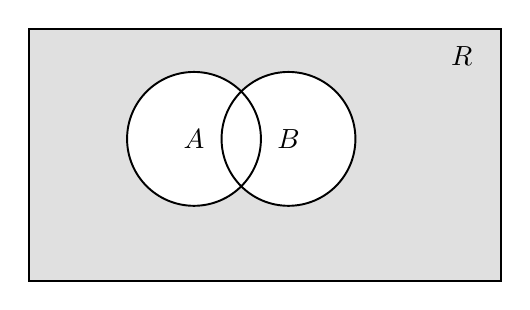
\begin{tikzpicture}[scale=1,line width=0.7pt]
\fill[black!12] (0,0) rectangle (6,3.2);
\fill[white] (2.1,1.8) circle (0.85);
\fill[white] (3.3,1.8) circle (0.85);
\draw (0,0) rectangle (6,3.2);
\draw (2.1,1.8) circle (0.85);
\draw (3.3,1.8) circle (0.85);
\node at (2.1,1.8) {$A$};
\node at (3.3,1.8) {$B$};
\node at (5.5,2.85) {$R$};
\end{tikzpicture}
\end{center}

（1）若集合 $C$ 表示图中阴影部分，用集合的运算式表示 $C$.

（2）求集合 $C$.

\ansspace*[12]

\ifanswer
\solbegin
\stepm{（1）}{由韦恩图得 $C=\overline{A\cup B}$.}
\stepm{（2）}{解 $\dfrac{x+1}{x-2}<-1$，则 $\dfrac{x+1}{x-2}+1<0$，即 $\dfrac{2x-1}{x-2}<0$，解得 $\dfrac12<x<2$，}
\step{故 $B=\left\{x\left|\dfrac12<x<2\right.\right\}$，所以 $A\cup B=\{x\mid-3\leqslant x<2\}$，}
\step{所以 $C=\overline{A\cup B}=\{x\mid x<-3\ \text{或}\ x\geqslant2\}$.}
\solend
\fi

\item 已知集合 $A=\{x\mid x^2-6x+8<0\}$，集合 $B=\{x\mid3m<x<1-m\}$.

（1）命题 $p:x\in A$，命题 $q:x\in B$，若 $p$ 是 $q$ 的充分条件，求实数 $m$ 的取值范围.

（2）若 $A\cap B=\varnothing$，求实数 $m$ 的取值范围.

\ansspace*[12]

\ifanswer
\solbegin
\stepm{（1）}{$x^2-6x+8<0\Rightarrow2<x<4\Rightarrow A=\{x\mid2<x<4\}$.}
\step{若 $p$ 是 $q$ 的充分条件，则 $A\subseteq B$，结合 $B$ 为非空集合，得 $\begin{cases}3m<1-m\\ 3m\leqslant2\\ 1-m\geqslant4\end{cases}$，}
\step{解得 $m\leqslant-3$，故 $m$ 的取值范围是 $(-\infty,-3]$；}
\stepm{（2）}{当 $B=\varnothing$ 时，$3m\geqslant1-m$，解得 $m\geqslant\dfrac14$，满足 $A\cap B=\varnothing$；}
\step{当 $B\neq\varnothing$ 时，$3m<1-m$ 即 $m<\dfrac14$，}
\step{要使交集为空，则 $1-m\leqslant2$ 或 $3m\geqslant4$，解得 $m\geqslant-1$，}
\step{结合 $m<\dfrac14$，得 $-1\leqslant m<\dfrac14$.}
\step{综上，$m\geqslant-1$，即 $m$ 的取值范围是 $[-1,+\infty)$.}
\solend
\fi

\item 设某企业每月生产电机 $x$ 台，根据企业月度报表知，每月总产值 $m$（万元）与总支出 $n$（万元）近似地满足下列关系：$m=\dfrac92x-\dfrac14$，$n=-\dfrac14x^2+5x+\dfrac74$，当 $m-n\geqslant0$ 时，称不亏损企业；当 $m-n<0$ 时，称亏损企业，且 $n-m$ 为亏损额.

（1）企业要成为不亏损企业，每月至少要生产多少台电机？

（2）当月总产值为多少时，企业亏损最严重，最大亏损额为多少？

\ansspace*[12]

\ifanswer
\solbegin
\stepm{（1）}{由题意得 $m-n\geqslant0$，即 $\dfrac92x-\dfrac14\geqslant-\dfrac14x^2+5x+\dfrac74$，}
\step{整理得 $x^2-2x-8\geqslant0$，解得 $x\geqslant4$ 或 $x\leqslant-2$（舍），}
\step{所以企业要成为不亏损企业，每月至少要生产 $4$ 台电机；}
\stepm{（2）}{由（1）得当 $0<x<4$ 时企业亏损，}
\step{亏损额 $n-m=\left(-\dfrac14x^2+5x+\dfrac74\right)-\left(\dfrac92x-\dfrac14\right)=-\dfrac14(x-1)^2+\dfrac94$，}
\step{所以当 $x=1$ 时，$n-m$ 取最大值 $\dfrac94$，}
\step{答：当月总产值为 $1$ 台时，企业亏损最严重，最大亏损额为 $\dfrac94$ 万元.}
\solend
\fi

\item 已知 $x_1$、$x_2$ 是一元二次方程 $4kx^2-4kx+k+1=0(k\neq0)$ 的两个实数根.

（1）是否存在实数 $k$，使 $x_1^2+x_2^2=\dfrac14$ 成立？若存在，求出 $k$ 的值，若不存在，请说明理由；

（2）是否存在整数 $k$，使 $\dfrac{x_1}{x_2}+\dfrac{x_2}{x_1}-2$ 的值为整数？若存在，求出 $k$ 的值，若不存在，请说明理由.

\ansspace*[14]

\ifanswer
\solbegin
\stepm{（1）}{因为 $x_1$、$x_2$ 是一元二次方程 $4kx^2-4kx+k+1=0(k\neq0)$ 的两个实数根，}
\step{所以 $\Delta=(-4k)^2-4\times4k(k+1)\geqslant0$，解得 $k\leqslant0$，}
\step{由韦达定理得 $\begin{cases}x_1+x_2=1\\ x_1x_2=\dfrac{k+1}{4k}\end{cases}$，}
\step{则 $x_1^2+x_2^2=(x_1+x_2)^2-2x_1x_2=\dfrac14$，}
\step{即 $1-2\times\dfrac{k+1}{4k}=\dfrac14$，解得 $k=2$，因为 $k\leqslant0$，所以不存在实数 $k$.}
\stepm{（2）}{$\dfrac{x_1}{x_2}+\dfrac{x_2}{x_1}-2=\dfrac{x_1^2+x_2^2}{x_1x_2}-2=\dfrac{(x_1+x_2)^2-2x_1x_2}{x_1x_2}-2=\dfrac{(x_1+x_2)^2}{x_1x_2}-4$}
\step{$=\dfrac{1}{\dfrac{k+1}{4k}}-4=\dfrac{4k}{k+1}-4=\dfrac{4k-4(k+1)}{k+1}=\dfrac{-4}{k+1}$，}
\step{由于 $\dfrac{x_1}{x_2}+\dfrac{x_2}{x_1}-2$ 的值为整数，即 $\dfrac{-4}{k+1}$ 的值为整数，}
\step{所以 $k+1$ 只能取 $\pm1$、$\pm2$、$\pm4$，}
\step{又 $k\leqslant0$，所以当 $k+1=\pm1$ 时，得出 $k=0$（舍）或 $k=-2$，}
\step{当 $k+1=\pm2$ 时，得出 $k=1$（舍）或 $k=-3$，}
\step{当 $k+1=\pm4$ 时，得出 $k=3$（舍）或 $k=-5$，}
\step{综上所述，若 $\dfrac{x_1}{x_2}+\dfrac{x_2}{x_1}-2$ 的值为整数，则 $k$ 的值为 $-2$ 或 $-3$ 或 $-5$.}
\solend
\fi

\item 已知集合 $A=\{a_1,a_2,\cdots,a_n\}(n\geqslant3)$，其中 $a_m\in\Z(m=1,2,\cdots,n)$. 若 $A$ 的子集 $T=\{a_i,a_j,a_k\}$ 满足 $2a_k=a_i+a_j$，则称 $T$ 具有性质 $P$. $A$ 的所有具有性质 $P$ 的子集 $T$ 的个数记为 $card_A(T)$.

（1）当 $A=\{4,-1,-2,1,-5\}$ 时，写出 $A$ 的所有具有性质 $P$ 的子集 $T$；

（2）当 $n=4$ 时，若 $a_1<a_2<a_3<a_4$，且 $card_A(T)=2$，证明：数对 $a_1$、$a_3$ 和 $a_2$、$a_4$ 中至少有一对中的两数奇偶性相同；

（3）当 $n=9$ 时，求 $card_A(T)$ 的最大值.

\ansspace*[14]

\ifanswer
\solbegin
\stepm{（1）}{集合 $A=\{4,-1,-2,1,-5\}$，元素按从小到大排列为 $-5$、$-2$、$-1$、$1$、$4$，}
\step{满足 $2a_k=a_i+a_j$ 的三元子集 $T$ 需满足其中一个元素是另外两个的平均数，}
\step{对于 $-5,-2,1$：$2\times(-2)=-4=-5+1$，满足条件，故 $T=\{-5,-2,1\}$，}
\step{对于 $-2,1,4$：$2\times1=2=-2+4$，满足条件，故 $T=\{-2,1,4\}$，}
\step{因此满足的子集有 $\{-5,-2,1\}$ 和 $\{-2,1,4\}$.}
\stepm{（2）}{假设数对 $(a_1,a_3)$ 和 $(a_2,a_4)$ 的两数奇偶性均不同，}
\step{即 $a_1$ 与 $a_3$ 一奇一偶，故 $a_1+a_3$ 为奇数，}
\step{$a_2$ 与 $a_4$ 一奇一偶，故 $a_2+a_4$ 为奇数，}
\step{集合 $A=\{a_1,a_2,a_3,a_4\}$ 的三元子集共 $\mathrm{C}_4^3=4$ 个：}
\step{$\{a_1,a_2,a_3\}$：若满足 $2a_2=a_1+a_3$，左边为偶数，右边为奇数，矛盾，故不满足；}
\step{$\{a_2,a_3,a_4\}$：若满足 $2a_3=a_2+a_4$，左边为偶数，右边为奇数，矛盾，故不满足；}
\step{$\{a_1,a_2,a_4\}$：需 $2a_2=a_1+a_4$；}
\step{$\{a_1,a_3,a_4\}$：需 $2a_3=a_1+a_4$.}
\step{若这两个子集都满足，则 $2a_2=2a_3\Rightarrow a_2=a_3$，与 $a_2<a_3$ 矛盾，}
\step{因此最多只有 $1$ 个子集满足条件，与 $card_A(T)=2$ 矛盾，故假设不成立，}
\step{即数对 $(a_1,a_3)$ 和 $(a_2,a_4)$ 中至少有一对的两数奇偶性相同.}
\stepm{（3）}{要最大化 $card_A(T)$，}
\step{集合 $A$ 应包含尽可能多的三元等差数列（即长度为 $3$ 的等差数列），}
\step{当 $A$ 为公差为 $1$ 的等差数列（如 $A=\{0,1,2,\cdots,8\}$）时，}
\step{三元等差数列的个数最多，}
\step{对于集合 $\{0,1,2,\cdots,8\}$，计算三元等差数列个数：}
\step{公差 $d=1$：$\{0,1,2\},\{1,2,3\},\cdots,\{6,7,8\}$，共 $7$ 个；}
\step{公差 $d=2$：$\{0,2,4\},\{1,3,5\},\cdots,\{4,6,8\}$，共 $5$ 个；}
\step{公差 $d=3$：$\{0,3,6\},\{1,4,7\},\{2,5,8\}$，共 $3$ 个；}
\step{公差 $d=4$：$\{0,4,8\}$，共 $1$ 个；}
\step{总个数为 $7+5+3+1=16$.}
\solend
\fi

\end{enumerate}

\end{document}
"
% 紧凑版：xelatex "\def\iscompact{1}% 高一89_宝山中学_10月月考.tex
%   —— 高一上数学“2026-2027 年宝山中学高一上 10 月月考”（讲评版）
% 试卷版：xelatex 高一89_宝山中学_10月月考.tex
% 答案版：xelatex "\def\isanswer{1}\input{高一89_宝山中学_10月月考.tex}"
% 紧凑版：xelatex "\def\iscompact{1}\input{高一89_宝山中学_10月月考.tex}"
%
% 原始材料：微信公众号“魔都数学加油站”文章，连载“27学年高一89”；
% 原文标题“27学年高一89——2026-2027年上海市宝山中学高一上10月月考”；
% 原文链接：https://mp.weixin.qq.com/s/DZ-Q-hfS4UulNW_vGWrZXw。
% 正文为 10 张 PNG 页（`原图/高一89_宝山中学_10月月考/01..10.png`），
% 尺寸混排（第 6 页为 2560×3620，其余为 4762×6735），均按页序读取。
%
% 篇幅与题号：原卷自第 3 题起编号（第 1、2 题不在原文内）。填空题 3—12（10 题）、
% 选择题 13—16（4 题）、解答题 17—21（5 题），共 19 题。
%
% 讲评版：第 4 题只印【答案】（“$x\leqslant2$ 或 $y\leqslant2$”），本稿只给 \ans{}；
% 其余 18 题印【解析】，其中选择题答案在解析末句“故选 C／B／A／A”。
% 第 17 题题干带一幅韦恩图（全集 $R$、集合 $A$、$B$ 与阴影部分），三版都出。
%
% 副标题：原卷未印副标题。本稿按内容标作“集合与常用逻辑用语、不等式”。
%
% 原卷笔误/存疑（均照录未改，正文对应处另有 % 注）：
%   ① 第 8 题题干“$k\in R$”与第 12 题“$n\in N$”按原卷用斜体字母排，本稿沿用
%      $\R$、$\N$ 记号（见“排版差异”③），此处不再视为笔误；
%   ② 第 9 题解析“故 $a$ 的取值范围是 $a<-1$ 或 $\dfrac13<a<\dfrac12$”，未把
%      $a<-1$ 写成区间，与同题前两行的写法不统一，属原卷写法，照录；
%   ③ 第 20 题 (1) 由 $\Delta\geqslant0$ 得“$k\leqslant0$”，与题设 $k\neq0$ 合看
%      应为 $k<0$；原卷写 $k\leqslant0$ 并以之舍去 $k=2$，结论不变，照录。
%
% 与原卷的排版差异：
%   ① 原卷每题下直接印【答案】/【解析】，本稿按全稿惯例将答案与解析置于答案版；
%   ② 原卷未印副标题，本稿补出；填空横线统一排 \blankline[4.4em]；
%   ③ 原卷数集记号排斜体 $R$、$Z$、$N$，本稿按全稿惯例改用 $\R$、$\Z$、$\N$；
%   ④ 第 17—21 题的子问用行内“（1）（2）（3）”段，解析中的子问标号用 \stepm；
%   ⑤ 解答题按惯例加 \ansspace；选择题括号排 \mbox{（\quad）}；
%   ⑥ 第 17 题的韦恩图原卷排在题干右侧、文字绕排，本稿改排为题干后的居中图
%      （TikZ 重绘：原图该处有公众号粉色水印斜压，按原图布局重绘，标注一致）。
%
% 行数核对：逐题数 \step/\stepm 条数，合计 119 条（Q3：2；Q4：0；Q5：3；Q6：4；
% Q7：2；Q8：3；Q9：4；Q10：5；Q11：8；Q12：4；Q13：5；Q14：7；Q15：9；Q16：5；
% Q17：4；Q18：8；Q19：7；Q20：13；Q21：26）。第 4 题只印【答案】，不计入 \step 账。
% 原卷解析的换行按语意合并，未逐行强拆。
%
\documentclass[a4paper,11pt]{article}
\usepackage{common}

\begin{document}

\examtitlest[7]{2026--2027 年宝山中学高一上 10 月月考}{集合与常用逻辑用语、不等式}

\bigsec{一、填空题}

\begin{enumerate}
\setcounter{enumi}{2}

\item 满足 $\{1,2\}\subseteq A\subseteq\{1,2,3,4,5\}$ 的集合共 $A$ 有\blankline[4.4em]个.

\ifanswer
\solbegin
\step{由题意得 $A=\{1,2\}$ 与 $\{3,4,5\}$ 的非空子集的并集，}
\step{而 $\{3,4,5\}$ 的子集有 $2^3=8$ 个，所以满足条件的 $A$ 有 $8$ 个.}
\solend
\fi

\item 用反证法证明命题：“若 $x+y>4$，则 $x>2$ 且 $y>2$”时，第一步应该假设\blankline[4.4em].

\ifanswer
\ans{$x\leqslant2$ 或 $y\leqslant2$}
\fi

\item 已知等式 $2x^2+3x+5=a(2x+1)(x+1)+c$ 恒成立，则 $a-c$ 的值为\blankline[4.4em].

\ifanswer
\solbegin
\step{因为 $2x^2+3x+5=a(2x+1)(x+1)+c$ 恒成立，}
\step{所以 $2x^2+3x+5=2ax^2+3ax+a+c$ 恒成立，}
\step{则 $\begin{cases}2=2a\\ 3=3a\\ 5=a+c\end{cases}$，得 $a=1$，$c=4$，所以 $a-c=-3$.}
\solend
\fi

\item 不等式 $\lvert3x-1\rvert<x$ 的解集\blankline[4.4em].

\ifanswer
\solbegin
\step{当 $x\leqslant0$ 时，不等式的解集为 $\varnothing$，}
\step{当 $x>0$ 时，$\lvert3x-1\rvert<x$，即 $(3x-1)^2<x^2$，}
\step{整理得 $8x^2-6x+1<0$，$(2x-1)(4x-1)<0$，解得 $\dfrac14<x<\dfrac12$，满足 $x>0$.}
\step{故解集为 $\left(\dfrac14,\dfrac12\right)$.}
\solend
\fi

\item 比较两个代数式的大小关系：$x^2+2y^2$\blankline[3em]$2xy+2y-1$.

\ifanswer
\solbegin
\step{$x^2+2y^2-(2xy+2y-1)=x^2-2xy+y^2+y^2-2y+1$}
\step{$=(x-y)^2+(y-1)^2\geqslant0$，所以 $x^2+2y^2\geqslant2xy+2y-1$.}
\solend
\fi

\item $k\in\R$，关于 $x$ 的不等式 $x^2+\sqrt2kx+2>0$ 的解集为全体实数，则 $k$ 的取值范围是\blankline[4.4em].

\ifanswer
\solbegin
\step{因为关于 $x$ 的不等式 $x^2+\sqrt2kx+2>0$ 的解集为全体实数，}
\step{所以 $\Delta=(\sqrt2k)^2-4\times1\times2=2k^2-8<0$，解得 $-2<k<2$，}
\step{即实数 $k$ 的取值范围是 $(-2,2)$.}
\solend
\fi

\item 在平面直角坐标系内，点 $\left(2a-1,\dfrac{3a-1}{a+1}\right)$ 在第二象限，则 $a$ 的取值范围是\blankline[4.4em].

\ifanswer
\solbegin
\step{由题意得 $\begin{cases}2a-1<0\\[0.2em]\dfrac{3a-1}{a+1}>0\end{cases}$，}
\step{由 $2a-1<0$，解得 $a<\dfrac12$；}
\step{由 $\dfrac{3a-1}{a+1}>0$，解得 $a<-1$ 或 $a>\dfrac13$；}
\step{故 $a$ 的取值范围是 $a<-1$ 或 $\dfrac13<a<\dfrac12$.}
\solend
\fi

\item 设集合 $A=\{x\mid x^2+x-6=0\}$，集合 $B=\{x\mid mx+1=0\}$，且 $A\cup B=A$，则 $m$ 的值组成的集合是\blankline[4.4em].

\ifanswer
\solbegin
\step{由题意得 $A=\{x\mid x^2+x-6=0\}=\{-3,2\}$，}
\step{由 $A\cup B=A$，得 $B\subseteq A$，}
\step{当 $m=0$ 时，$B=\varnothing$，满足题意，}
\step{当 $m\neq0$ 时，$B=\left\{-\dfrac1m\right\}$，所以 $-\dfrac1m=2$ 或 $-\dfrac1m=-3$，所以 $m=-\dfrac12$ 或 $m=\dfrac13$，}
\step{综上所述，$m$ 的值组成的集合是 $\left\{0,-\dfrac12,\dfrac13\right\}$.}
\solend
\fi

\item 甲、乙两人解关于 $x$ 的不等式 $x^2+bx+c<0$，甲写错了 $b$，正确计算后得到的解为 $\{x\mid1<x<2\}$；乙写错了 $c$，正确计算后得到的解为 $\{x\mid-4<x<1\}$. 那么不等式 $\dfrac{bx+c}{x-2}<0$ 的解为\blankline[4.4em].

\ifanswer
\solbegin
\step{由 $x^2+bx+c<0$ 的解为 $\{x\mid1<x<2\}$，}
\step{则 $1$ 和 $2$ 是方程 $x^2+bx+c=0$ 的两个根，}
\step{甲写错了 $b$，但 $c$ 是正确的，所以 $c=1\times2=2$；}
\step{由 $x^2+bx+c<0$ 的解为 $\{x\mid-4<x<1\}$，}
\step{则 $-4$ 和 $1$ 是方程 $x^2+bx+c=0$ 的两个根，}
\step{乙写错了 $c$，但 $b$ 是正确的，所以 $-b=-4+1=-3$，即 $b=3$.}
\step{由 $\dfrac{bx+c}{x-2}<0$，得 $\dfrac{3x+2}{x-2}<0$，即 $(3x+2)(x-2)<0$，解得 $-\dfrac23<x<2$，}
\step{所以不等式 $\dfrac{bx+c}{x-2}<0$ 的解为 $\left\{x\left|-\dfrac23<x<2\right.\right\}$.}
\solend
\fi

\item 已知集合 $M$ 的元素均为正整数，定义集合 $M$ 的“变项和”为：将 $M$ 中每个元素 $m$ 都乘以 $(-1)^m$ 后再求和. 若集合 $A=\{n\mid1\leqslant n\leqslant10,n\in\N\}$，则集合 $A$ 的所有非空子集的“变项和”的总和为\blankline[4.4em].

\ifanswer
\solbegin
\step{$A$ 集合的所有非空子集中，每个元素出现的次数都是 $(2^{10}-1)-(2^9-1)=2^9$，}
\step{则集合 $A$ 的所有非空子集的“变项和”的总和}
\step{为 $1\times(-1)^1\times2^9+2\times(-1)^2\times2^9+\cdots+10\times(-1)^{10}\times2^9$}
\step{$=(-1+2-3+4-\cdots-9+10)\times2^9=5\times2^9=2560$.}
\solend
\fi

\end{enumerate}

\bigsec{二、选择题}

\begin{enumerate}
\setcounter{enumi}{12}

\item 下列命题中正确的是\mbox{（\quad）}

\keepwithprev
A. 若 $a>b$，则 $\dfrac1a<\dfrac1b$\qquad B. 若 $a>b$，则 $a^2>b^2$

C. 若 $a>\lvert b\rvert$，则 $a>b$\qquad D. 若 $a>b$，则 $ac^2>bc^2$

\ifanswer
\solbegin
\step{对于 $AB$ 选项，取 $a=1$，$b=-1$，$a>b$，$\dfrac1a>\dfrac1b$，$a^2=b^2$，}
\step{所以 $AB$ 选项错误；}
\step{对于 $C$ 选项，由 $a>\lvert b\rvert$，$\lvert b\rvert\geqslant b$，得 $a>b$，所以 $C$ 选项正确；}
\step{对于 $D$ 选项，取 $c=0$，则 $ac^2=0=bc^2$，所以 $D$ 选项错误.}
\step{故选 $C$.}
\solend
\fi

\item 下面关于集合的表示正确的个数是\mbox{（\quad）}

①$\{1,2,3\}=\{3,2,1\}$；\quad ②$\{(x,y)\mid x-y=1\}=\{y\mid y=x-1\}$；

③$\{x\mid x\geqslant2,x\in\N\}=\{y\mid y\geqslant2,y\in\Z\}$；\quad ④$\{x\mid x+2y=1\}\neq\left\{y\left|y=-\dfrac12x+\dfrac12\right.\right\}$.

\keepwithprev
A. $1$\qquad B. $2$\qquad C. $3$\qquad D. $4$

\ifanswer
\solbegin
\step{对于①，由元素的无序性得①正确；}
\step{对于②，$\{(x,y)\mid x-y=1\}$ 表示点集，$\{y\mid y=x-1\}$ 表示数集，故②错误；}
\step{对于③，$\{x\mid x\geqslant2,x\in\N\}$ 表示大于等于 $2$ 的整数，}
\step{$\{y\mid y\geqslant2,y\in\Z\}$ 也表示大于等于 $2$ 的整数，故③正确；}
\step{对于④，$\{x\mid x+2y=1\}=\R$，$\left\{y\left|y=-\dfrac12x+\dfrac12\right.\right\}=\R$，}
\step{所以 $\{x\mid x+2y=1\}=\left\{y\left|y=-\dfrac12x+\dfrac12\right.\right\}$，故④错误，}
\step{所以正确的个数是 $2$ 个. 故选 $B$.}
\solend
\fi

\item 已知命题 $P$：方程 $ax^2+bx+c=0$ 有两个不相等实根；命题 $Q$：不等式 $ax^2+bx+c>0$ 与 $ax^2+bx+c<0$ 均有解，则命题 $P$ 成立是命题 $Q$ 成立的\mbox{（\quad）}条件.

\keepwithprev
A. 充分非必要条件\qquad B. 必要非充分条件

C. 充要条件\qquad D. 既非充分又非必要条件

\ifanswer
\solbegin
\step{若 $P$ 成立，即方程 $ax^2+bx+c=0$ 有两个不相等实根，}
\step{此时 $\begin{cases}a\neq0\\ \Delta=b^2-4ac>0\end{cases}$；}
\step{若 $Q$ 成立，即不等式 $ax^2+bx+c>0$ 与 $ax^2+bx+c<0$ 均有解，有两种情况：}
\step{①不等式是一元二次不等式，}
\step{此时不等式所对应的二次函数的图像与 $x$ 轴有两个交点，}
\step{满足 $\begin{cases}a\neq0\\ \Delta=b^2-4ac>0\end{cases}$；}
\step{②不等式是一元一次不等式，此时 $\begin{cases}a=0\\ b\neq0\end{cases}$，}
\step{因此，由 $P$ 能推出 $Q$ 成立，但是由 $Q$ 不能推出 $P$ 成立，}
\step{即 $P$ 是 $Q$ 的充分非必要条件. 故选 $A$.}
\solend
\fi

\item 甲、乙同去加油站加油两次，两次汽油单价分别为 $x$、$y$ 元/升（$x\neq y$）. 甲每次加固定金额的油，乙每次加固定体积的油. 哪种方式更经济实惠呢？\mbox{（\quad）}

\keepwithprev
A. 加固定金额的方式\qquad B. 加固定体积的方式

C. 两种方案一样\qquad D. 要视具体价格而定

\ifanswer
\solbegin
\step{设两次加油的油价分别为 $x$、$y$（$x$、$y>0$，且 $x\neq y$），}
\step{乙每次加油的量为 $a$（$a>0$）；甲每次加油的钱数为 $b$（$b>0$），}
\step{则乙平均油价为 $\dfrac{ax+ay}{2a}=\dfrac{x+y}{2}$，甲平均油价为 $\dfrac{2b}{\dfrac bx+\dfrac by}=\dfrac2{\dfrac1x+\dfrac1y}=\dfrac{2xy}{x+y}$，}
\step{因为 $x\neq y$，所以 $\dfrac{x+y}{2}-\dfrac{2xy}{x+y}=\dfrac{(x-y)^2}{2(x+y)}>0$，所以 $\dfrac{x+y}{2}>\dfrac{2xy}{x+y}$，}
\step{即甲方案更经济. 故选 $A$.}
\solend
\fi

\end{enumerate}

\bigsec{三、解答题}

\begin{enumerate}
\setcounter{enumi}{16}

\item 已知全集 $U=\R$，集合 $A=\{x\mid-3\leqslant x\leqslant1\}$，$B=\left\{x\left|\dfrac{x+1}{x-2}<-1\right.\right\}$.

\begin{center}
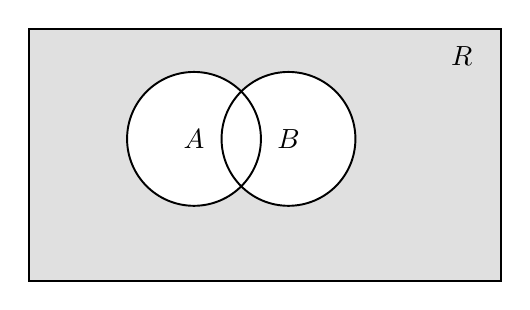
\begin{tikzpicture}[scale=1,line width=0.7pt]
\fill[black!12] (0,0) rectangle (6,3.2);
\fill[white] (2.1,1.8) circle (0.85);
\fill[white] (3.3,1.8) circle (0.85);
\draw (0,0) rectangle (6,3.2);
\draw (2.1,1.8) circle (0.85);
\draw (3.3,1.8) circle (0.85);
\node at (2.1,1.8) {$A$};
\node at (3.3,1.8) {$B$};
\node at (5.5,2.85) {$R$};
\end{tikzpicture}
\end{center}

（1）若集合 $C$ 表示图中阴影部分，用集合的运算式表示 $C$.

（2）求集合 $C$.

\ansspace*[12]

\ifanswer
\solbegin
\stepm{（1）}{由韦恩图得 $C=\overline{A\cup B}$.}
\stepm{（2）}{解 $\dfrac{x+1}{x-2}<-1$，则 $\dfrac{x+1}{x-2}+1<0$，即 $\dfrac{2x-1}{x-2}<0$，解得 $\dfrac12<x<2$，}
\step{故 $B=\left\{x\left|\dfrac12<x<2\right.\right\}$，所以 $A\cup B=\{x\mid-3\leqslant x<2\}$，}
\step{所以 $C=\overline{A\cup B}=\{x\mid x<-3\ \text{或}\ x\geqslant2\}$.}
\solend
\fi

\item 已知集合 $A=\{x\mid x^2-6x+8<0\}$，集合 $B=\{x\mid3m<x<1-m\}$.

（1）命题 $p:x\in A$，命题 $q:x\in B$，若 $p$ 是 $q$ 的充分条件，求实数 $m$ 的取值范围.

（2）若 $A\cap B=\varnothing$，求实数 $m$ 的取值范围.

\ansspace*[12]

\ifanswer
\solbegin
\stepm{（1）}{$x^2-6x+8<0\Rightarrow2<x<4\Rightarrow A=\{x\mid2<x<4\}$.}
\step{若 $p$ 是 $q$ 的充分条件，则 $A\subseteq B$，结合 $B$ 为非空集合，得 $\begin{cases}3m<1-m\\ 3m\leqslant2\\ 1-m\geqslant4\end{cases}$，}
\step{解得 $m\leqslant-3$，故 $m$ 的取值范围是 $(-\infty,-3]$；}
\stepm{（2）}{当 $B=\varnothing$ 时，$3m\geqslant1-m$，解得 $m\geqslant\dfrac14$，满足 $A\cap B=\varnothing$；}
\step{当 $B\neq\varnothing$ 时，$3m<1-m$ 即 $m<\dfrac14$，}
\step{要使交集为空，则 $1-m\leqslant2$ 或 $3m\geqslant4$，解得 $m\geqslant-1$，}
\step{结合 $m<\dfrac14$，得 $-1\leqslant m<\dfrac14$.}
\step{综上，$m\geqslant-1$，即 $m$ 的取值范围是 $[-1,+\infty)$.}
\solend
\fi

\item 设某企业每月生产电机 $x$ 台，根据企业月度报表知，每月总产值 $m$（万元）与总支出 $n$（万元）近似地满足下列关系：$m=\dfrac92x-\dfrac14$，$n=-\dfrac14x^2+5x+\dfrac74$，当 $m-n\geqslant0$ 时，称不亏损企业；当 $m-n<0$ 时，称亏损企业，且 $n-m$ 为亏损额.

（1）企业要成为不亏损企业，每月至少要生产多少台电机？

（2）当月总产值为多少时，企业亏损最严重，最大亏损额为多少？

\ansspace*[12]

\ifanswer
\solbegin
\stepm{（1）}{由题意得 $m-n\geqslant0$，即 $\dfrac92x-\dfrac14\geqslant-\dfrac14x^2+5x+\dfrac74$，}
\step{整理得 $x^2-2x-8\geqslant0$，解得 $x\geqslant4$ 或 $x\leqslant-2$（舍），}
\step{所以企业要成为不亏损企业，每月至少要生产 $4$ 台电机；}
\stepm{（2）}{由（1）得当 $0<x<4$ 时企业亏损，}
\step{亏损额 $n-m=\left(-\dfrac14x^2+5x+\dfrac74\right)-\left(\dfrac92x-\dfrac14\right)=-\dfrac14(x-1)^2+\dfrac94$，}
\step{所以当 $x=1$ 时，$n-m$ 取最大值 $\dfrac94$，}
\step{答：当月总产值为 $1$ 台时，企业亏损最严重，最大亏损额为 $\dfrac94$ 万元.}
\solend
\fi

\item 已知 $x_1$、$x_2$ 是一元二次方程 $4kx^2-4kx+k+1=0(k\neq0)$ 的两个实数根.

（1）是否存在实数 $k$，使 $x_1^2+x_2^2=\dfrac14$ 成立？若存在，求出 $k$ 的值，若不存在，请说明理由；

（2）是否存在整数 $k$，使 $\dfrac{x_1}{x_2}+\dfrac{x_2}{x_1}-2$ 的值为整数？若存在，求出 $k$ 的值，若不存在，请说明理由.

\ansspace*[14]

\ifanswer
\solbegin
\stepm{（1）}{因为 $x_1$、$x_2$ 是一元二次方程 $4kx^2-4kx+k+1=0(k\neq0)$ 的两个实数根，}
\step{所以 $\Delta=(-4k)^2-4\times4k(k+1)\geqslant0$，解得 $k\leqslant0$，}
\step{由韦达定理得 $\begin{cases}x_1+x_2=1\\ x_1x_2=\dfrac{k+1}{4k}\end{cases}$，}
\step{则 $x_1^2+x_2^2=(x_1+x_2)^2-2x_1x_2=\dfrac14$，}
\step{即 $1-2\times\dfrac{k+1}{4k}=\dfrac14$，解得 $k=2$，因为 $k\leqslant0$，所以不存在实数 $k$.}
\stepm{（2）}{$\dfrac{x_1}{x_2}+\dfrac{x_2}{x_1}-2=\dfrac{x_1^2+x_2^2}{x_1x_2}-2=\dfrac{(x_1+x_2)^2-2x_1x_2}{x_1x_2}-2=\dfrac{(x_1+x_2)^2}{x_1x_2}-4$}
\step{$=\dfrac{1}{\dfrac{k+1}{4k}}-4=\dfrac{4k}{k+1}-4=\dfrac{4k-4(k+1)}{k+1}=\dfrac{-4}{k+1}$，}
\step{由于 $\dfrac{x_1}{x_2}+\dfrac{x_2}{x_1}-2$ 的值为整数，即 $\dfrac{-4}{k+1}$ 的值为整数，}
\step{所以 $k+1$ 只能取 $\pm1$、$\pm2$、$\pm4$，}
\step{又 $k\leqslant0$，所以当 $k+1=\pm1$ 时，得出 $k=0$（舍）或 $k=-2$，}
\step{当 $k+1=\pm2$ 时，得出 $k=1$（舍）或 $k=-3$，}
\step{当 $k+1=\pm4$ 时，得出 $k=3$（舍）或 $k=-5$，}
\step{综上所述，若 $\dfrac{x_1}{x_2}+\dfrac{x_2}{x_1}-2$ 的值为整数，则 $k$ 的值为 $-2$ 或 $-3$ 或 $-5$.}
\solend
\fi

\item 已知集合 $A=\{a_1,a_2,\cdots,a_n\}(n\geqslant3)$，其中 $a_m\in\Z(m=1,2,\cdots,n)$. 若 $A$ 的子集 $T=\{a_i,a_j,a_k\}$ 满足 $2a_k=a_i+a_j$，则称 $T$ 具有性质 $P$. $A$ 的所有具有性质 $P$ 的子集 $T$ 的个数记为 $card_A(T)$.

（1）当 $A=\{4,-1,-2,1,-5\}$ 时，写出 $A$ 的所有具有性质 $P$ 的子集 $T$；

（2）当 $n=4$ 时，若 $a_1<a_2<a_3<a_4$，且 $card_A(T)=2$，证明：数对 $a_1$、$a_3$ 和 $a_2$、$a_4$ 中至少有一对中的两数奇偶性相同；

（3）当 $n=9$ 时，求 $card_A(T)$ 的最大值.

\ansspace*[14]

\ifanswer
\solbegin
\stepm{（1）}{集合 $A=\{4,-1,-2,1,-5\}$，元素按从小到大排列为 $-5$、$-2$、$-1$、$1$、$4$，}
\step{满足 $2a_k=a_i+a_j$ 的三元子集 $T$ 需满足其中一个元素是另外两个的平均数，}
\step{对于 $-5,-2,1$：$2\times(-2)=-4=-5+1$，满足条件，故 $T=\{-5,-2,1\}$，}
\step{对于 $-2,1,4$：$2\times1=2=-2+4$，满足条件，故 $T=\{-2,1,4\}$，}
\step{因此满足的子集有 $\{-5,-2,1\}$ 和 $\{-2,1,4\}$.}
\stepm{（2）}{假设数对 $(a_1,a_3)$ 和 $(a_2,a_4)$ 的两数奇偶性均不同，}
\step{即 $a_1$ 与 $a_3$ 一奇一偶，故 $a_1+a_3$ 为奇数，}
\step{$a_2$ 与 $a_4$ 一奇一偶，故 $a_2+a_4$ 为奇数，}
\step{集合 $A=\{a_1,a_2,a_3,a_4\}$ 的三元子集共 $\mathrm{C}_4^3=4$ 个：}
\step{$\{a_1,a_2,a_3\}$：若满足 $2a_2=a_1+a_3$，左边为偶数，右边为奇数，矛盾，故不满足；}
\step{$\{a_2,a_3,a_4\}$：若满足 $2a_3=a_2+a_4$，左边为偶数，右边为奇数，矛盾，故不满足；}
\step{$\{a_1,a_2,a_4\}$：需 $2a_2=a_1+a_4$；}
\step{$\{a_1,a_3,a_4\}$：需 $2a_3=a_1+a_4$.}
\step{若这两个子集都满足，则 $2a_2=2a_3\Rightarrow a_2=a_3$，与 $a_2<a_3$ 矛盾，}
\step{因此最多只有 $1$ 个子集满足条件，与 $card_A(T)=2$ 矛盾，故假设不成立，}
\step{即数对 $(a_1,a_3)$ 和 $(a_2,a_4)$ 中至少有一对的两数奇偶性相同.}
\stepm{（3）}{要最大化 $card_A(T)$，}
\step{集合 $A$ 应包含尽可能多的三元等差数列（即长度为 $3$ 的等差数列），}
\step{当 $A$ 为公差为 $1$ 的等差数列（如 $A=\{0,1,2,\cdots,8\}$）时，}
\step{三元等差数列的个数最多，}
\step{对于集合 $\{0,1,2,\cdots,8\}$，计算三元等差数列个数：}
\step{公差 $d=1$：$\{0,1,2\},\{1,2,3\},\cdots,\{6,7,8\}$，共 $7$ 个；}
\step{公差 $d=2$：$\{0,2,4\},\{1,3,5\},\cdots,\{4,6,8\}$，共 $5$ 个；}
\step{公差 $d=3$：$\{0,3,6\},\{1,4,7\},\{2,5,8\}$，共 $3$ 个；}
\step{公差 $d=4$：$\{0,4,8\}$，共 $1$ 个；}
\step{总个数为 $7+5+3+1=16$.}
\solend
\fi

\end{enumerate}

\end{document}
"
%
% 原始材料：微信公众号“魔都数学加油站”文章，连载“27学年高一89”；
% 原文标题“27学年高一89——2026-2027年上海市宝山中学高一上10月月考”；
% 原文链接：https://mp.weixin.qq.com/s/DZ-Q-hfS4UulNW_vGWrZXw。
% 正文为 10 张 PNG 页（`原图/高一89_宝山中学_10月月考/01..10.png`），
% 尺寸混排（第 6 页为 2560×3620，其余为 4762×6735），均按页序读取。
%
% 篇幅与题号：原卷自第 3 题起编号（第 1、2 题不在原文内）。填空题 3—12（10 题）、
% 选择题 13—16（4 题）、解答题 17—21（5 题），共 19 题。
%
% 讲评版：第 4 题只印【答案】（“$x\leqslant2$ 或 $y\leqslant2$”），本稿只给 \ans{}；
% 其余 18 题印【解析】，其中选择题答案在解析末句“故选 C／B／A／A”。
% 第 17 题题干带一幅韦恩图（全集 $R$、集合 $A$、$B$ 与阴影部分），三版都出。
%
% 副标题：原卷未印副标题。本稿按内容标作“集合与常用逻辑用语、不等式”。
%
% 原卷笔误/存疑（均照录未改，正文对应处另有 % 注）：
%   ① 第 8 题题干“$k\in R$”与第 12 题“$n\in N$”按原卷用斜体字母排，本稿沿用
%      $\R$、$\N$ 记号（见“排版差异”③），此处不再视为笔误；
%   ② 第 9 题解析“故 $a$ 的取值范围是 $a<-1$ 或 $\dfrac13<a<\dfrac12$”，未把
%      $a<-1$ 写成区间，与同题前两行的写法不统一，属原卷写法，照录；
%   ③ 第 20 题 (1) 由 $\Delta\geqslant0$ 得“$k\leqslant0$”，与题设 $k\neq0$ 合看
%      应为 $k<0$；原卷写 $k\leqslant0$ 并以之舍去 $k=2$，结论不变，照录。
%
% 与原卷的排版差异：
%   ① 原卷每题下直接印【答案】/【解析】，本稿按全稿惯例将答案与解析置于答案版；
%   ② 原卷未印副标题，本稿补出；填空横线统一排 \blankline[4.4em]；
%   ③ 原卷数集记号排斜体 $R$、$Z$、$N$，本稿按全稿惯例改用 $\R$、$\Z$、$\N$；
%   ④ 第 17—21 题的子问用行内“（1）（2）（3）”段，解析中的子问标号用 \stepm；
%   ⑤ 解答题按惯例加 \ansspace；选择题括号排 \mbox{（\quad）}；
%   ⑥ 第 17 题的韦恩图原卷排在题干右侧、文字绕排，本稿改排为题干后的居中图
%      （TikZ 重绘：原图该处有公众号粉色水印斜压，按原图布局重绘，标注一致）。
%
% 行数核对：逐题数 \step/\stepm 条数，合计 119 条（Q3：2；Q4：0；Q5：3；Q6：4；
% Q7：2；Q8：3；Q9：4；Q10：5；Q11：8；Q12：4；Q13：5；Q14：7；Q15：9；Q16：5；
% Q17：4；Q18：8；Q19：7；Q20：13；Q21：26）。第 4 题只印【答案】，不计入 \step 账。
% 原卷解析的换行按语意合并，未逐行强拆。
%
\documentclass[a4paper,11pt]{article}
\usepackage{common}

\begin{document}

\examtitlest[7]{2026--2027 年宝山中学高一上 10 月月考}{集合与常用逻辑用语、不等式}

\bigsec{一、填空题}

\begin{enumerate}
\setcounter{enumi}{2}

\item 满足 $\{1,2\}\subseteq A\subseteq\{1,2,3,4,5\}$ 的集合共 $A$ 有\blankline[4.4em]个.

\ifanswer
\solbegin
\step{由题意得 $A=\{1,2\}$ 与 $\{3,4,5\}$ 的非空子集的并集，}
\step{而 $\{3,4,5\}$ 的子集有 $2^3=8$ 个，所以满足条件的 $A$ 有 $8$ 个.}
\solend
\fi

\item 用反证法证明命题：“若 $x+y>4$，则 $x>2$ 且 $y>2$”时，第一步应该假设\blankline[4.4em].

\ifanswer
\ans{$x\leqslant2$ 或 $y\leqslant2$}
\fi

\item 已知等式 $2x^2+3x+5=a(2x+1)(x+1)+c$ 恒成立，则 $a-c$ 的值为\blankline[4.4em].

\ifanswer
\solbegin
\step{因为 $2x^2+3x+5=a(2x+1)(x+1)+c$ 恒成立，}
\step{所以 $2x^2+3x+5=2ax^2+3ax+a+c$ 恒成立，}
\step{则 $\begin{cases}2=2a\\ 3=3a\\ 5=a+c\end{cases}$，得 $a=1$，$c=4$，所以 $a-c=-3$.}
\solend
\fi

\item 不等式 $\lvert3x-1\rvert<x$ 的解集\blankline[4.4em].

\ifanswer
\solbegin
\step{当 $x\leqslant0$ 时，不等式的解集为 $\varnothing$，}
\step{当 $x>0$ 时，$\lvert3x-1\rvert<x$，即 $(3x-1)^2<x^2$，}
\step{整理得 $8x^2-6x+1<0$，$(2x-1)(4x-1)<0$，解得 $\dfrac14<x<\dfrac12$，满足 $x>0$.}
\step{故解集为 $\left(\dfrac14,\dfrac12\right)$.}
\solend
\fi

\item 比较两个代数式的大小关系：$x^2+2y^2$\blankline[3em]$2xy+2y-1$.

\ifanswer
\solbegin
\step{$x^2+2y^2-(2xy+2y-1)=x^2-2xy+y^2+y^2-2y+1$}
\step{$=(x-y)^2+(y-1)^2\geqslant0$，所以 $x^2+2y^2\geqslant2xy+2y-1$.}
\solend
\fi

\item $k\in\R$，关于 $x$ 的不等式 $x^2+\sqrt2kx+2>0$ 的解集为全体实数，则 $k$ 的取值范围是\blankline[4.4em].

\ifanswer
\solbegin
\step{因为关于 $x$ 的不等式 $x^2+\sqrt2kx+2>0$ 的解集为全体实数，}
\step{所以 $\Delta=(\sqrt2k)^2-4\times1\times2=2k^2-8<0$，解得 $-2<k<2$，}
\step{即实数 $k$ 的取值范围是 $(-2,2)$.}
\solend
\fi

\item 在平面直角坐标系内，点 $\left(2a-1,\dfrac{3a-1}{a+1}\right)$ 在第二象限，则 $a$ 的取值范围是\blankline[4.4em].

\ifanswer
\solbegin
\step{由题意得 $\begin{cases}2a-1<0\\[0.2em]\dfrac{3a-1}{a+1}>0\end{cases}$，}
\step{由 $2a-1<0$，解得 $a<\dfrac12$；}
\step{由 $\dfrac{3a-1}{a+1}>0$，解得 $a<-1$ 或 $a>\dfrac13$；}
\step{故 $a$ 的取值范围是 $a<-1$ 或 $\dfrac13<a<\dfrac12$.}
\solend
\fi

\item 设集合 $A=\{x\mid x^2+x-6=0\}$，集合 $B=\{x\mid mx+1=0\}$，且 $A\cup B=A$，则 $m$ 的值组成的集合是\blankline[4.4em].

\ifanswer
\solbegin
\step{由题意得 $A=\{x\mid x^2+x-6=0\}=\{-3,2\}$，}
\step{由 $A\cup B=A$，得 $B\subseteq A$，}
\step{当 $m=0$ 时，$B=\varnothing$，满足题意，}
\step{当 $m\neq0$ 时，$B=\left\{-\dfrac1m\right\}$，所以 $-\dfrac1m=2$ 或 $-\dfrac1m=-3$，所以 $m=-\dfrac12$ 或 $m=\dfrac13$，}
\step{综上所述，$m$ 的值组成的集合是 $\left\{0,-\dfrac12,\dfrac13\right\}$.}
\solend
\fi

\item 甲、乙两人解关于 $x$ 的不等式 $x^2+bx+c<0$，甲写错了 $b$，正确计算后得到的解为 $\{x\mid1<x<2\}$；乙写错了 $c$，正确计算后得到的解为 $\{x\mid-4<x<1\}$. 那么不等式 $\dfrac{bx+c}{x-2}<0$ 的解为\blankline[4.4em].

\ifanswer
\solbegin
\step{由 $x^2+bx+c<0$ 的解为 $\{x\mid1<x<2\}$，}
\step{则 $1$ 和 $2$ 是方程 $x^2+bx+c=0$ 的两个根，}
\step{甲写错了 $b$，但 $c$ 是正确的，所以 $c=1\times2=2$；}
\step{由 $x^2+bx+c<0$ 的解为 $\{x\mid-4<x<1\}$，}
\step{则 $-4$ 和 $1$ 是方程 $x^2+bx+c=0$ 的两个根，}
\step{乙写错了 $c$，但 $b$ 是正确的，所以 $-b=-4+1=-3$，即 $b=3$.}
\step{由 $\dfrac{bx+c}{x-2}<0$，得 $\dfrac{3x+2}{x-2}<0$，即 $(3x+2)(x-2)<0$，解得 $-\dfrac23<x<2$，}
\step{所以不等式 $\dfrac{bx+c}{x-2}<0$ 的解为 $\left\{x\left|-\dfrac23<x<2\right.\right\}$.}
\solend
\fi

\item 已知集合 $M$ 的元素均为正整数，定义集合 $M$ 的“变项和”为：将 $M$ 中每个元素 $m$ 都乘以 $(-1)^m$ 后再求和. 若集合 $A=\{n\mid1\leqslant n\leqslant10,n\in\N\}$，则集合 $A$ 的所有非空子集的“变项和”的总和为\blankline[4.4em].

\ifanswer
\solbegin
\step{$A$ 集合的所有非空子集中，每个元素出现的次数都是 $(2^{10}-1)-(2^9-1)=2^9$，}
\step{则集合 $A$ 的所有非空子集的“变项和”的总和}
\step{为 $1\times(-1)^1\times2^9+2\times(-1)^2\times2^9+\cdots+10\times(-1)^{10}\times2^9$}
\step{$=(-1+2-3+4-\cdots-9+10)\times2^9=5\times2^9=2560$.}
\solend
\fi

\end{enumerate}

\bigsec{二、选择题}

\begin{enumerate}
\setcounter{enumi}{12}

\item 下列命题中正确的是\mbox{（\quad）}

\keepwithprev
A. 若 $a>b$，则 $\dfrac1a<\dfrac1b$\qquad B. 若 $a>b$，则 $a^2>b^2$

C. 若 $a>\lvert b\rvert$，则 $a>b$\qquad D. 若 $a>b$，则 $ac^2>bc^2$

\ifanswer
\solbegin
\step{对于 $AB$ 选项，取 $a=1$，$b=-1$，$a>b$，$\dfrac1a>\dfrac1b$，$a^2=b^2$，}
\step{所以 $AB$ 选项错误；}
\step{对于 $C$ 选项，由 $a>\lvert b\rvert$，$\lvert b\rvert\geqslant b$，得 $a>b$，所以 $C$ 选项正确；}
\step{对于 $D$ 选项，取 $c=0$，则 $ac^2=0=bc^2$，所以 $D$ 选项错误.}
\step{故选 $C$.}
\solend
\fi

\item 下面关于集合的表示正确的个数是\mbox{（\quad）}

①$\{1,2,3\}=\{3,2,1\}$；\quad ②$\{(x,y)\mid x-y=1\}=\{y\mid y=x-1\}$；

③$\{x\mid x\geqslant2,x\in\N\}=\{y\mid y\geqslant2,y\in\Z\}$；\quad ④$\{x\mid x+2y=1\}\neq\left\{y\left|y=-\dfrac12x+\dfrac12\right.\right\}$.

\keepwithprev
A. $1$\qquad B. $2$\qquad C. $3$\qquad D. $4$

\ifanswer
\solbegin
\step{对于①，由元素的无序性得①正确；}
\step{对于②，$\{(x,y)\mid x-y=1\}$ 表示点集，$\{y\mid y=x-1\}$ 表示数集，故②错误；}
\step{对于③，$\{x\mid x\geqslant2,x\in\N\}$ 表示大于等于 $2$ 的整数，}
\step{$\{y\mid y\geqslant2,y\in\Z\}$ 也表示大于等于 $2$ 的整数，故③正确；}
\step{对于④，$\{x\mid x+2y=1\}=\R$，$\left\{y\left|y=-\dfrac12x+\dfrac12\right.\right\}=\R$，}
\step{所以 $\{x\mid x+2y=1\}=\left\{y\left|y=-\dfrac12x+\dfrac12\right.\right\}$，故④错误，}
\step{所以正确的个数是 $2$ 个. 故选 $B$.}
\solend
\fi

\item 已知命题 $P$：方程 $ax^2+bx+c=0$ 有两个不相等实根；命题 $Q$：不等式 $ax^2+bx+c>0$ 与 $ax^2+bx+c<0$ 均有解，则命题 $P$ 成立是命题 $Q$ 成立的\mbox{（\quad）}条件.

\keepwithprev
A. 充分非必要条件\qquad B. 必要非充分条件

C. 充要条件\qquad D. 既非充分又非必要条件

\ifanswer
\solbegin
\step{若 $P$ 成立，即方程 $ax^2+bx+c=0$ 有两个不相等实根，}
\step{此时 $\begin{cases}a\neq0\\ \Delta=b^2-4ac>0\end{cases}$；}
\step{若 $Q$ 成立，即不等式 $ax^2+bx+c>0$ 与 $ax^2+bx+c<0$ 均有解，有两种情况：}
\step{①不等式是一元二次不等式，}
\step{此时不等式所对应的二次函数的图像与 $x$ 轴有两个交点，}
\step{满足 $\begin{cases}a\neq0\\ \Delta=b^2-4ac>0\end{cases}$；}
\step{②不等式是一元一次不等式，此时 $\begin{cases}a=0\\ b\neq0\end{cases}$，}
\step{因此，由 $P$ 能推出 $Q$ 成立，但是由 $Q$ 不能推出 $P$ 成立，}
\step{即 $P$ 是 $Q$ 的充分非必要条件. 故选 $A$.}
\solend
\fi

\item 甲、乙同去加油站加油两次，两次汽油单价分别为 $x$、$y$ 元/升（$x\neq y$）. 甲每次加固定金额的油，乙每次加固定体积的油. 哪种方式更经济实惠呢？\mbox{（\quad）}

\keepwithprev
A. 加固定金额的方式\qquad B. 加固定体积的方式

C. 两种方案一样\qquad D. 要视具体价格而定

\ifanswer
\solbegin
\step{设两次加油的油价分别为 $x$、$y$（$x$、$y>0$，且 $x\neq y$），}
\step{乙每次加油的量为 $a$（$a>0$）；甲每次加油的钱数为 $b$（$b>0$），}
\step{则乙平均油价为 $\dfrac{ax+ay}{2a}=\dfrac{x+y}{2}$，甲平均油价为 $\dfrac{2b}{\dfrac bx+\dfrac by}=\dfrac2{\dfrac1x+\dfrac1y}=\dfrac{2xy}{x+y}$，}
\step{因为 $x\neq y$，所以 $\dfrac{x+y}{2}-\dfrac{2xy}{x+y}=\dfrac{(x-y)^2}{2(x+y)}>0$，所以 $\dfrac{x+y}{2}>\dfrac{2xy}{x+y}$，}
\step{即甲方案更经济. 故选 $A$.}
\solend
\fi

\end{enumerate}

\bigsec{三、解答题}

\begin{enumerate}
\setcounter{enumi}{16}

\item 已知全集 $U=\R$，集合 $A=\{x\mid-3\leqslant x\leqslant1\}$，$B=\left\{x\left|\dfrac{x+1}{x-2}<-1\right.\right\}$.

\begin{center}
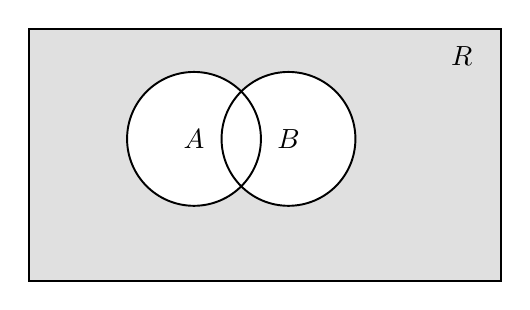
\begin{tikzpicture}[scale=1,line width=0.7pt]
\fill[black!12] (0,0) rectangle (6,3.2);
\fill[white] (2.1,1.8) circle (0.85);
\fill[white] (3.3,1.8) circle (0.85);
\draw (0,0) rectangle (6,3.2);
\draw (2.1,1.8) circle (0.85);
\draw (3.3,1.8) circle (0.85);
\node at (2.1,1.8) {$A$};
\node at (3.3,1.8) {$B$};
\node at (5.5,2.85) {$R$};
\end{tikzpicture}
\end{center}

（1）若集合 $C$ 表示图中阴影部分，用集合的运算式表示 $C$.

（2）求集合 $C$.

\ansspace*[12]

\ifanswer
\solbegin
\stepm{（1）}{由韦恩图得 $C=\overline{A\cup B}$.}
\stepm{（2）}{解 $\dfrac{x+1}{x-2}<-1$，则 $\dfrac{x+1}{x-2}+1<0$，即 $\dfrac{2x-1}{x-2}<0$，解得 $\dfrac12<x<2$，}
\step{故 $B=\left\{x\left|\dfrac12<x<2\right.\right\}$，所以 $A\cup B=\{x\mid-3\leqslant x<2\}$，}
\step{所以 $C=\overline{A\cup B}=\{x\mid x<-3\ \text{或}\ x\geqslant2\}$.}
\solend
\fi

\item 已知集合 $A=\{x\mid x^2-6x+8<0\}$，集合 $B=\{x\mid3m<x<1-m\}$.

（1）命题 $p:x\in A$，命题 $q:x\in B$，若 $p$ 是 $q$ 的充分条件，求实数 $m$ 的取值范围.

（2）若 $A\cap B=\varnothing$，求实数 $m$ 的取值范围.

\ansspace*[12]

\ifanswer
\solbegin
\stepm{（1）}{$x^2-6x+8<0\Rightarrow2<x<4\Rightarrow A=\{x\mid2<x<4\}$.}
\step{若 $p$ 是 $q$ 的充分条件，则 $A\subseteq B$，结合 $B$ 为非空集合，得 $\begin{cases}3m<1-m\\ 3m\leqslant2\\ 1-m\geqslant4\end{cases}$，}
\step{解得 $m\leqslant-3$，故 $m$ 的取值范围是 $(-\infty,-3]$；}
\stepm{（2）}{当 $B=\varnothing$ 时，$3m\geqslant1-m$，解得 $m\geqslant\dfrac14$，满足 $A\cap B=\varnothing$；}
\step{当 $B\neq\varnothing$ 时，$3m<1-m$ 即 $m<\dfrac14$，}
\step{要使交集为空，则 $1-m\leqslant2$ 或 $3m\geqslant4$，解得 $m\geqslant-1$，}
\step{结合 $m<\dfrac14$，得 $-1\leqslant m<\dfrac14$.}
\step{综上，$m\geqslant-1$，即 $m$ 的取值范围是 $[-1,+\infty)$.}
\solend
\fi

\item 设某企业每月生产电机 $x$ 台，根据企业月度报表知，每月总产值 $m$（万元）与总支出 $n$（万元）近似地满足下列关系：$m=\dfrac92x-\dfrac14$，$n=-\dfrac14x^2+5x+\dfrac74$，当 $m-n\geqslant0$ 时，称不亏损企业；当 $m-n<0$ 时，称亏损企业，且 $n-m$ 为亏损额.

（1）企业要成为不亏损企业，每月至少要生产多少台电机？

（2）当月总产值为多少时，企业亏损最严重，最大亏损额为多少？

\ansspace*[12]

\ifanswer
\solbegin
\stepm{（1）}{由题意得 $m-n\geqslant0$，即 $\dfrac92x-\dfrac14\geqslant-\dfrac14x^2+5x+\dfrac74$，}
\step{整理得 $x^2-2x-8\geqslant0$，解得 $x\geqslant4$ 或 $x\leqslant-2$（舍），}
\step{所以企业要成为不亏损企业，每月至少要生产 $4$ 台电机；}
\stepm{（2）}{由（1）得当 $0<x<4$ 时企业亏损，}
\step{亏损额 $n-m=\left(-\dfrac14x^2+5x+\dfrac74\right)-\left(\dfrac92x-\dfrac14\right)=-\dfrac14(x-1)^2+\dfrac94$，}
\step{所以当 $x=1$ 时，$n-m$ 取最大值 $\dfrac94$，}
\step{答：当月总产值为 $1$ 台时，企业亏损最严重，最大亏损额为 $\dfrac94$ 万元.}
\solend
\fi

\item 已知 $x_1$、$x_2$ 是一元二次方程 $4kx^2-4kx+k+1=0(k\neq0)$ 的两个实数根.

（1）是否存在实数 $k$，使 $x_1^2+x_2^2=\dfrac14$ 成立？若存在，求出 $k$ 的值，若不存在，请说明理由；

（2）是否存在整数 $k$，使 $\dfrac{x_1}{x_2}+\dfrac{x_2}{x_1}-2$ 的值为整数？若存在，求出 $k$ 的值，若不存在，请说明理由.

\ansspace*[14]

\ifanswer
\solbegin
\stepm{（1）}{因为 $x_1$、$x_2$ 是一元二次方程 $4kx^2-4kx+k+1=0(k\neq0)$ 的两个实数根，}
\step{所以 $\Delta=(-4k)^2-4\times4k(k+1)\geqslant0$，解得 $k\leqslant0$，}
\step{由韦达定理得 $\begin{cases}x_1+x_2=1\\ x_1x_2=\dfrac{k+1}{4k}\end{cases}$，}
\step{则 $x_1^2+x_2^2=(x_1+x_2)^2-2x_1x_2=\dfrac14$，}
\step{即 $1-2\times\dfrac{k+1}{4k}=\dfrac14$，解得 $k=2$，因为 $k\leqslant0$，所以不存在实数 $k$.}
\stepm{（2）}{$\dfrac{x_1}{x_2}+\dfrac{x_2}{x_1}-2=\dfrac{x_1^2+x_2^2}{x_1x_2}-2=\dfrac{(x_1+x_2)^2-2x_1x_2}{x_1x_2}-2=\dfrac{(x_1+x_2)^2}{x_1x_2}-4$}
\step{$=\dfrac{1}{\dfrac{k+1}{4k}}-4=\dfrac{4k}{k+1}-4=\dfrac{4k-4(k+1)}{k+1}=\dfrac{-4}{k+1}$，}
\step{由于 $\dfrac{x_1}{x_2}+\dfrac{x_2}{x_1}-2$ 的值为整数，即 $\dfrac{-4}{k+1}$ 的值为整数，}
\step{所以 $k+1$ 只能取 $\pm1$、$\pm2$、$\pm4$，}
\step{又 $k\leqslant0$，所以当 $k+1=\pm1$ 时，得出 $k=0$（舍）或 $k=-2$，}
\step{当 $k+1=\pm2$ 时，得出 $k=1$（舍）或 $k=-3$，}
\step{当 $k+1=\pm4$ 时，得出 $k=3$（舍）或 $k=-5$，}
\step{综上所述，若 $\dfrac{x_1}{x_2}+\dfrac{x_2}{x_1}-2$ 的值为整数，则 $k$ 的值为 $-2$ 或 $-3$ 或 $-5$.}
\solend
\fi

\item 已知集合 $A=\{a_1,a_2,\cdots,a_n\}(n\geqslant3)$，其中 $a_m\in\Z(m=1,2,\cdots,n)$. 若 $A$ 的子集 $T=\{a_i,a_j,a_k\}$ 满足 $2a_k=a_i+a_j$，则称 $T$ 具有性质 $P$. $A$ 的所有具有性质 $P$ 的子集 $T$ 的个数记为 $card_A(T)$.

（1）当 $A=\{4,-1,-2,1,-5\}$ 时，写出 $A$ 的所有具有性质 $P$ 的子集 $T$；

（2）当 $n=4$ 时，若 $a_1<a_2<a_3<a_4$，且 $card_A(T)=2$，证明：数对 $a_1$、$a_3$ 和 $a_2$、$a_4$ 中至少有一对中的两数奇偶性相同；

（3）当 $n=9$ 时，求 $card_A(T)$ 的最大值.

\ansspace*[14]

\ifanswer
\solbegin
\stepm{（1）}{集合 $A=\{4,-1,-2,1,-5\}$，元素按从小到大排列为 $-5$、$-2$、$-1$、$1$、$4$，}
\step{满足 $2a_k=a_i+a_j$ 的三元子集 $T$ 需满足其中一个元素是另外两个的平均数，}
\step{对于 $-5,-2,1$：$2\times(-2)=-4=-5+1$，满足条件，故 $T=\{-5,-2,1\}$，}
\step{对于 $-2,1,4$：$2\times1=2=-2+4$，满足条件，故 $T=\{-2,1,4\}$，}
\step{因此满足的子集有 $\{-5,-2,1\}$ 和 $\{-2,1,4\}$.}
\stepm{（2）}{假设数对 $(a_1,a_3)$ 和 $(a_2,a_4)$ 的两数奇偶性均不同，}
\step{即 $a_1$ 与 $a_3$ 一奇一偶，故 $a_1+a_3$ 为奇数，}
\step{$a_2$ 与 $a_4$ 一奇一偶，故 $a_2+a_4$ 为奇数，}
\step{集合 $A=\{a_1,a_2,a_3,a_4\}$ 的三元子集共 $\mathrm{C}_4^3=4$ 个：}
\step{$\{a_1,a_2,a_3\}$：若满足 $2a_2=a_1+a_3$，左边为偶数，右边为奇数，矛盾，故不满足；}
\step{$\{a_2,a_3,a_4\}$：若满足 $2a_3=a_2+a_4$，左边为偶数，右边为奇数，矛盾，故不满足；}
\step{$\{a_1,a_2,a_4\}$：需 $2a_2=a_1+a_4$；}
\step{$\{a_1,a_3,a_4\}$：需 $2a_3=a_1+a_4$.}
\step{若这两个子集都满足，则 $2a_2=2a_3\Rightarrow a_2=a_3$，与 $a_2<a_3$ 矛盾，}
\step{因此最多只有 $1$ 个子集满足条件，与 $card_A(T)=2$ 矛盾，故假设不成立，}
\step{即数对 $(a_1,a_3)$ 和 $(a_2,a_4)$ 中至少有一对的两数奇偶性相同.}
\stepm{（3）}{要最大化 $card_A(T)$，}
\step{集合 $A$ 应包含尽可能多的三元等差数列（即长度为 $3$ 的等差数列），}
\step{当 $A$ 为公差为 $1$ 的等差数列（如 $A=\{0,1,2,\cdots,8\}$）时，}
\step{三元等差数列的个数最多，}
\step{对于集合 $\{0,1,2,\cdots,8\}$，计算三元等差数列个数：}
\step{公差 $d=1$：$\{0,1,2\},\{1,2,3\},\cdots,\{6,7,8\}$，共 $7$ 个；}
\step{公差 $d=2$：$\{0,2,4\},\{1,3,5\},\cdots,\{4,6,8\}$，共 $5$ 个；}
\step{公差 $d=3$：$\{0,3,6\},\{1,4,7\},\{2,5,8\}$，共 $3$ 个；}
\step{公差 $d=4$：$\{0,4,8\}$，共 $1$ 个；}
\step{总个数为 $7+5+3+1=16$.}
\solend
\fi

\end{enumerate}

\end{document}
"
%
% 原始材料：微信公众号“魔都数学加油站”文章，连载“27学年高一89”；
% 原文标题“27学年高一89——2026-2027年上海市宝山中学高一上10月月考”；
% 原文链接：https://mp.weixin.qq.com/s/DZ-Q-hfS4UulNW_vGWrZXw。
% 正文为 10 张 PNG 页（`原图/高一89_宝山中学_10月月考/01..10.png`），
% 尺寸混排（第 6 页为 2560×3620，其余为 4762×6735），均按页序读取。
%
% 篇幅与题号：原卷自第 3 题起编号（第 1、2 题不在原文内）。填空题 3—12（10 题）、
% 选择题 13—16（4 题）、解答题 17—21（5 题），共 19 题。
%
% 讲评版：第 4 题只印【答案】（“$x\leqslant2$ 或 $y\leqslant2$”），本稿只给 \ans{}；
% 其余 18 题印【解析】，其中选择题答案在解析末句“故选 C／B／A／A”。
% 第 17 题题干带一幅韦恩图（全集 $R$、集合 $A$、$B$ 与阴影部分），三版都出。
%
% 副标题：原卷未印副标题。本稿按内容标作“集合与常用逻辑用语、不等式”。
%
% 原卷笔误/存疑（均照录未改，正文对应处另有 % 注）：
%   ① 第 8 题题干“$k\in R$”与第 12 题“$n\in N$”按原卷用斜体字母排，本稿沿用
%      $\R$、$\N$ 记号（见“排版差异”③），此处不再视为笔误；
%   ② 第 9 题解析“故 $a$ 的取值范围是 $a<-1$ 或 $\dfrac13<a<\dfrac12$”，未把
%      $a<-1$ 写成区间，与同题前两行的写法不统一，属原卷写法，照录；
%   ③ 第 20 题 (1) 由 $\Delta\geqslant0$ 得“$k\leqslant0$”，与题设 $k\neq0$ 合看
%      应为 $k<0$；原卷写 $k\leqslant0$ 并以之舍去 $k=2$，结论不变，照录。
%
% 与原卷的排版差异：
%   ① 原卷每题下直接印【答案】/【解析】，本稿按全稿惯例将答案与解析置于答案版；
%   ② 原卷未印副标题，本稿补出；填空横线统一排 \blankline[4.4em]；
%   ③ 原卷数集记号排斜体 $R$、$Z$、$N$，本稿按全稿惯例改用 $\R$、$\Z$、$\N$；
%   ④ 第 17—21 题的子问用行内“（1）（2）（3）”段，解析中的子问标号用 \stepm；
%   ⑤ 解答题按惯例加 \ansspace；选择题括号排 \mbox{（\quad）}；
%   ⑥ 第 17 题的韦恩图原卷排在题干右侧、文字绕排，本稿改排为题干后的居中图
%      （TikZ 重绘：原图该处有公众号粉色水印斜压，按原图布局重绘，标注一致）。
%
% 行数核对：逐题数 \step/\stepm 条数，合计 119 条（Q3：2；Q4：0；Q5：3；Q6：4；
% Q7：2；Q8：3；Q9：4；Q10：5；Q11：8；Q12：4；Q13：5；Q14：7；Q15：9；Q16：5；
% Q17：4；Q18：8；Q19：7；Q20：13；Q21：26）。第 4 题只印【答案】，不计入 \step 账。
% 原卷解析的换行按语意合并，未逐行强拆。
%
\documentclass[a4paper,11pt]{article}
\usepackage{common}

\begin{document}

\examtitlest[7]{2026--2027 年宝山中学高一上 10 月月考}{集合与常用逻辑用语、不等式}

\bigsec{一、填空题}

\begin{enumerate}
\setcounter{enumi}{2}

\item 满足 $\{1,2\}\subseteq A\subseteq\{1,2,3,4,5\}$ 的集合共 $A$ 有\blankline[4.4em]个.

\ifanswer
\solbegin
\step{由题意得 $A=\{1,2\}$ 与 $\{3,4,5\}$ 的非空子集的并集，}
\step{而 $\{3,4,5\}$ 的子集有 $2^3=8$ 个，所以满足条件的 $A$ 有 $8$ 个.}
\solend
\fi

\item 用反证法证明命题：“若 $x+y>4$，则 $x>2$ 且 $y>2$”时，第一步应该假设\blankline[4.4em].

\ifanswer
\ans{$x\leqslant2$ 或 $y\leqslant2$}
\fi

\item 已知等式 $2x^2+3x+5=a(2x+1)(x+1)+c$ 恒成立，则 $a-c$ 的值为\blankline[4.4em].

\ifanswer
\solbegin
\step{因为 $2x^2+3x+5=a(2x+1)(x+1)+c$ 恒成立，}
\step{所以 $2x^2+3x+5=2ax^2+3ax+a+c$ 恒成立，}
\step{则 $\begin{cases}2=2a\\ 3=3a\\ 5=a+c\end{cases}$，得 $a=1$，$c=4$，所以 $a-c=-3$.}
\solend
\fi

\item 不等式 $\lvert3x-1\rvert<x$ 的解集\blankline[4.4em].

\ifanswer
\solbegin
\step{当 $x\leqslant0$ 时，不等式的解集为 $\varnothing$，}
\step{当 $x>0$ 时，$\lvert3x-1\rvert<x$，即 $(3x-1)^2<x^2$，}
\step{整理得 $8x^2-6x+1<0$，$(2x-1)(4x-1)<0$，解得 $\dfrac14<x<\dfrac12$，满足 $x>0$.}
\step{故解集为 $\left(\dfrac14,\dfrac12\right)$.}
\solend
\fi

\item 比较两个代数式的大小关系：$x^2+2y^2$\blankline[3em]$2xy+2y-1$.

\ifanswer
\solbegin
\step{$x^2+2y^2-(2xy+2y-1)=x^2-2xy+y^2+y^2-2y+1$}
\step{$=(x-y)^2+(y-1)^2\geqslant0$，所以 $x^2+2y^2\geqslant2xy+2y-1$.}
\solend
\fi

\item $k\in\R$，关于 $x$ 的不等式 $x^2+\sqrt2kx+2>0$ 的解集为全体实数，则 $k$ 的取值范围是\blankline[4.4em].

\ifanswer
\solbegin
\step{因为关于 $x$ 的不等式 $x^2+\sqrt2kx+2>0$ 的解集为全体实数，}
\step{所以 $\Delta=(\sqrt2k)^2-4\times1\times2=2k^2-8<0$，解得 $-2<k<2$，}
\step{即实数 $k$ 的取值范围是 $(-2,2)$.}
\solend
\fi

\item 在平面直角坐标系内，点 $\left(2a-1,\dfrac{3a-1}{a+1}\right)$ 在第二象限，则 $a$ 的取值范围是\blankline[4.4em].

\ifanswer
\solbegin
\step{由题意得 $\begin{cases}2a-1<0\\[0.2em]\dfrac{3a-1}{a+1}>0\end{cases}$，}
\step{由 $2a-1<0$，解得 $a<\dfrac12$；}
\step{由 $\dfrac{3a-1}{a+1}>0$，解得 $a<-1$ 或 $a>\dfrac13$；}
\step{故 $a$ 的取值范围是 $a<-1$ 或 $\dfrac13<a<\dfrac12$.}
\solend
\fi

\item 设集合 $A=\{x\mid x^2+x-6=0\}$，集合 $B=\{x\mid mx+1=0\}$，且 $A\cup B=A$，则 $m$ 的值组成的集合是\blankline[4.4em].

\ifanswer
\solbegin
\step{由题意得 $A=\{x\mid x^2+x-6=0\}=\{-3,2\}$，}
\step{由 $A\cup B=A$，得 $B\subseteq A$，}
\step{当 $m=0$ 时，$B=\varnothing$，满足题意，}
\step{当 $m\neq0$ 时，$B=\left\{-\dfrac1m\right\}$，所以 $-\dfrac1m=2$ 或 $-\dfrac1m=-3$，所以 $m=-\dfrac12$ 或 $m=\dfrac13$，}
\step{综上所述，$m$ 的值组成的集合是 $\left\{0,-\dfrac12,\dfrac13\right\}$.}
\solend
\fi

\item 甲、乙两人解关于 $x$ 的不等式 $x^2+bx+c<0$，甲写错了 $b$，正确计算后得到的解为 $\{x\mid1<x<2\}$；乙写错了 $c$，正确计算后得到的解为 $\{x\mid-4<x<1\}$. 那么不等式 $\dfrac{bx+c}{x-2}<0$ 的解为\blankline[4.4em].

\ifanswer
\solbegin
\step{由 $x^2+bx+c<0$ 的解为 $\{x\mid1<x<2\}$，}
\step{则 $1$ 和 $2$ 是方程 $x^2+bx+c=0$ 的两个根，}
\step{甲写错了 $b$，但 $c$ 是正确的，所以 $c=1\times2=2$；}
\step{由 $x^2+bx+c<0$ 的解为 $\{x\mid-4<x<1\}$，}
\step{则 $-4$ 和 $1$ 是方程 $x^2+bx+c=0$ 的两个根，}
\step{乙写错了 $c$，但 $b$ 是正确的，所以 $-b=-4+1=-3$，即 $b=3$.}
\step{由 $\dfrac{bx+c}{x-2}<0$，得 $\dfrac{3x+2}{x-2}<0$，即 $(3x+2)(x-2)<0$，解得 $-\dfrac23<x<2$，}
\step{所以不等式 $\dfrac{bx+c}{x-2}<0$ 的解为 $\left\{x\left|-\dfrac23<x<2\right.\right\}$.}
\solend
\fi

\item 已知集合 $M$ 的元素均为正整数，定义集合 $M$ 的“变项和”为：将 $M$ 中每个元素 $m$ 都乘以 $(-1)^m$ 后再求和. 若集合 $A=\{n\mid1\leqslant n\leqslant10,n\in\N\}$，则集合 $A$ 的所有非空子集的“变项和”的总和为\blankline[4.4em].

\ifanswer
\solbegin
\step{$A$ 集合的所有非空子集中，每个元素出现的次数都是 $(2^{10}-1)-(2^9-1)=2^9$，}
\step{则集合 $A$ 的所有非空子集的“变项和”的总和}
\step{为 $1\times(-1)^1\times2^9+2\times(-1)^2\times2^9+\cdots+10\times(-1)^{10}\times2^9$}
\step{$=(-1+2-3+4-\cdots-9+10)\times2^9=5\times2^9=2560$.}
\solend
\fi

\end{enumerate}

\bigsec{二、选择题}

\begin{enumerate}
\setcounter{enumi}{12}

\item 下列命题中正确的是\mbox{（\quad）}

\keepwithprev
A. 若 $a>b$，则 $\dfrac1a<\dfrac1b$\qquad B. 若 $a>b$，则 $a^2>b^2$

C. 若 $a>\lvert b\rvert$，则 $a>b$\qquad D. 若 $a>b$，则 $ac^2>bc^2$

\ifanswer
\solbegin
\step{对于 $AB$ 选项，取 $a=1$，$b=-1$，$a>b$，$\dfrac1a>\dfrac1b$，$a^2=b^2$，}
\step{所以 $AB$ 选项错误；}
\step{对于 $C$ 选项，由 $a>\lvert b\rvert$，$\lvert b\rvert\geqslant b$，得 $a>b$，所以 $C$ 选项正确；}
\step{对于 $D$ 选项，取 $c=0$，则 $ac^2=0=bc^2$，所以 $D$ 选项错误.}
\step{故选 $C$.}
\solend
\fi

\item 下面关于集合的表示正确的个数是\mbox{（\quad）}

①$\{1,2,3\}=\{3,2,1\}$；\quad ②$\{(x,y)\mid x-y=1\}=\{y\mid y=x-1\}$；

③$\{x\mid x\geqslant2,x\in\N\}=\{y\mid y\geqslant2,y\in\Z\}$；\quad ④$\{x\mid x+2y=1\}\neq\left\{y\left|y=-\dfrac12x+\dfrac12\right.\right\}$.

\keepwithprev
A. $1$\qquad B. $2$\qquad C. $3$\qquad D. $4$

\ifanswer
\solbegin
\step{对于①，由元素的无序性得①正确；}
\step{对于②，$\{(x,y)\mid x-y=1\}$ 表示点集，$\{y\mid y=x-1\}$ 表示数集，故②错误；}
\step{对于③，$\{x\mid x\geqslant2,x\in\N\}$ 表示大于等于 $2$ 的整数，}
\step{$\{y\mid y\geqslant2,y\in\Z\}$ 也表示大于等于 $2$ 的整数，故③正确；}
\step{对于④，$\{x\mid x+2y=1\}=\R$，$\left\{y\left|y=-\dfrac12x+\dfrac12\right.\right\}=\R$，}
\step{所以 $\{x\mid x+2y=1\}=\left\{y\left|y=-\dfrac12x+\dfrac12\right.\right\}$，故④错误，}
\step{所以正确的个数是 $2$ 个. 故选 $B$.}
\solend
\fi

\item 已知命题 $P$：方程 $ax^2+bx+c=0$ 有两个不相等实根；命题 $Q$：不等式 $ax^2+bx+c>0$ 与 $ax^2+bx+c<0$ 均有解，则命题 $P$ 成立是命题 $Q$ 成立的\mbox{（\quad）}条件.

\keepwithprev
A. 充分非必要条件\qquad B. 必要非充分条件

C. 充要条件\qquad D. 既非充分又非必要条件

\ifanswer
\solbegin
\step{若 $P$ 成立，即方程 $ax^2+bx+c=0$ 有两个不相等实根，}
\step{此时 $\begin{cases}a\neq0\\ \Delta=b^2-4ac>0\end{cases}$；}
\step{若 $Q$ 成立，即不等式 $ax^2+bx+c>0$ 与 $ax^2+bx+c<0$ 均有解，有两种情况：}
\step{①不等式是一元二次不等式，}
\step{此时不等式所对应的二次函数的图像与 $x$ 轴有两个交点，}
\step{满足 $\begin{cases}a\neq0\\ \Delta=b^2-4ac>0\end{cases}$；}
\step{②不等式是一元一次不等式，此时 $\begin{cases}a=0\\ b\neq0\end{cases}$，}
\step{因此，由 $P$ 能推出 $Q$ 成立，但是由 $Q$ 不能推出 $P$ 成立，}
\step{即 $P$ 是 $Q$ 的充分非必要条件. 故选 $A$.}
\solend
\fi

\item 甲、乙同去加油站加油两次，两次汽油单价分别为 $x$、$y$ 元/升（$x\neq y$）. 甲每次加固定金额的油，乙每次加固定体积的油. 哪种方式更经济实惠呢？\mbox{（\quad）}

\keepwithprev
A. 加固定金额的方式\qquad B. 加固定体积的方式

C. 两种方案一样\qquad D. 要视具体价格而定

\ifanswer
\solbegin
\step{设两次加油的油价分别为 $x$、$y$（$x$、$y>0$，且 $x\neq y$），}
\step{乙每次加油的量为 $a$（$a>0$）；甲每次加油的钱数为 $b$（$b>0$），}
\step{则乙平均油价为 $\dfrac{ax+ay}{2a}=\dfrac{x+y}{2}$，甲平均油价为 $\dfrac{2b}{\dfrac bx+\dfrac by}=\dfrac2{\dfrac1x+\dfrac1y}=\dfrac{2xy}{x+y}$，}
\step{因为 $x\neq y$，所以 $\dfrac{x+y}{2}-\dfrac{2xy}{x+y}=\dfrac{(x-y)^2}{2(x+y)}>0$，所以 $\dfrac{x+y}{2}>\dfrac{2xy}{x+y}$，}
\step{即甲方案更经济. 故选 $A$.}
\solend
\fi

\end{enumerate}

\bigsec{三、解答题}

\begin{enumerate}
\setcounter{enumi}{16}

\item 已知全集 $U=\R$，集合 $A=\{x\mid-3\leqslant x\leqslant1\}$，$B=\left\{x\left|\dfrac{x+1}{x-2}<-1\right.\right\}$.

\begin{center}
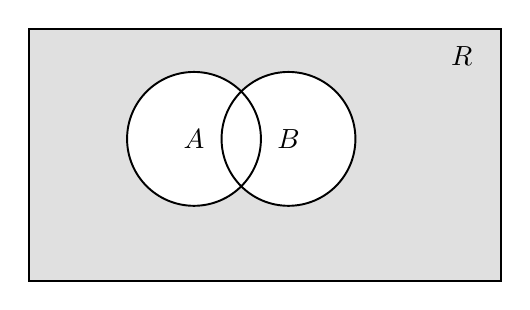
\begin{tikzpicture}[scale=1,line width=0.7pt]
\fill[black!12] (0,0) rectangle (6,3.2);
\fill[white] (2.1,1.8) circle (0.85);
\fill[white] (3.3,1.8) circle (0.85);
\draw (0,0) rectangle (6,3.2);
\draw (2.1,1.8) circle (0.85);
\draw (3.3,1.8) circle (0.85);
\node at (2.1,1.8) {$A$};
\node at (3.3,1.8) {$B$};
\node at (5.5,2.85) {$R$};
\end{tikzpicture}
\end{center}

（1）若集合 $C$ 表示图中阴影部分，用集合的运算式表示 $C$.

（2）求集合 $C$.

\ansspace*[12]

\ifanswer
\solbegin
\stepm{（1）}{由韦恩图得 $C=\overline{A\cup B}$.}
\stepm{（2）}{解 $\dfrac{x+1}{x-2}<-1$，则 $\dfrac{x+1}{x-2}+1<0$，即 $\dfrac{2x-1}{x-2}<0$，解得 $\dfrac12<x<2$，}
\step{故 $B=\left\{x\left|\dfrac12<x<2\right.\right\}$，所以 $A\cup B=\{x\mid-3\leqslant x<2\}$，}
\step{所以 $C=\overline{A\cup B}=\{x\mid x<-3\ \text{或}\ x\geqslant2\}$.}
\solend
\fi

\item 已知集合 $A=\{x\mid x^2-6x+8<0\}$，集合 $B=\{x\mid3m<x<1-m\}$.

（1）命题 $p:x\in A$，命题 $q:x\in B$，若 $p$ 是 $q$ 的充分条件，求实数 $m$ 的取值范围.

（2）若 $A\cap B=\varnothing$，求实数 $m$ 的取值范围.

\ansspace*[12]

\ifanswer
\solbegin
\stepm{（1）}{$x^2-6x+8<0\Rightarrow2<x<4\Rightarrow A=\{x\mid2<x<4\}$.}
\step{若 $p$ 是 $q$ 的充分条件，则 $A\subseteq B$，结合 $B$ 为非空集合，得 $\begin{cases}3m<1-m\\ 3m\leqslant2\\ 1-m\geqslant4\end{cases}$，}
\step{解得 $m\leqslant-3$，故 $m$ 的取值范围是 $(-\infty,-3]$；}
\stepm{（2）}{当 $B=\varnothing$ 时，$3m\geqslant1-m$，解得 $m\geqslant\dfrac14$，满足 $A\cap B=\varnothing$；}
\step{当 $B\neq\varnothing$ 时，$3m<1-m$ 即 $m<\dfrac14$，}
\step{要使交集为空，则 $1-m\leqslant2$ 或 $3m\geqslant4$，解得 $m\geqslant-1$，}
\step{结合 $m<\dfrac14$，得 $-1\leqslant m<\dfrac14$.}
\step{综上，$m\geqslant-1$，即 $m$ 的取值范围是 $[-1,+\infty)$.}
\solend
\fi

\item 设某企业每月生产电机 $x$ 台，根据企业月度报表知，每月总产值 $m$（万元）与总支出 $n$（万元）近似地满足下列关系：$m=\dfrac92x-\dfrac14$，$n=-\dfrac14x^2+5x+\dfrac74$，当 $m-n\geqslant0$ 时，称不亏损企业；当 $m-n<0$ 时，称亏损企业，且 $n-m$ 为亏损额.

（1）企业要成为不亏损企业，每月至少要生产多少台电机？

（2）当月总产值为多少时，企业亏损最严重，最大亏损额为多少？

\ansspace*[12]

\ifanswer
\solbegin
\stepm{（1）}{由题意得 $m-n\geqslant0$，即 $\dfrac92x-\dfrac14\geqslant-\dfrac14x^2+5x+\dfrac74$，}
\step{整理得 $x^2-2x-8\geqslant0$，解得 $x\geqslant4$ 或 $x\leqslant-2$（舍），}
\step{所以企业要成为不亏损企业，每月至少要生产 $4$ 台电机；}
\stepm{（2）}{由（1）得当 $0<x<4$ 时企业亏损，}
\step{亏损额 $n-m=\left(-\dfrac14x^2+5x+\dfrac74\right)-\left(\dfrac92x-\dfrac14\right)=-\dfrac14(x-1)^2+\dfrac94$，}
\step{所以当 $x=1$ 时，$n-m$ 取最大值 $\dfrac94$，}
\step{答：当月总产值为 $1$ 台时，企业亏损最严重，最大亏损额为 $\dfrac94$ 万元.}
\solend
\fi

\item 已知 $x_1$、$x_2$ 是一元二次方程 $4kx^2-4kx+k+1=0(k\neq0)$ 的两个实数根.

（1）是否存在实数 $k$，使 $x_1^2+x_2^2=\dfrac14$ 成立？若存在，求出 $k$ 的值，若不存在，请说明理由；

（2）是否存在整数 $k$，使 $\dfrac{x_1}{x_2}+\dfrac{x_2}{x_1}-2$ 的值为整数？若存在，求出 $k$ 的值，若不存在，请说明理由.

\ansspace*[14]

\ifanswer
\solbegin
\stepm{（1）}{因为 $x_1$、$x_2$ 是一元二次方程 $4kx^2-4kx+k+1=0(k\neq0)$ 的两个实数根，}
\step{所以 $\Delta=(-4k)^2-4\times4k(k+1)\geqslant0$，解得 $k\leqslant0$，}
\step{由韦达定理得 $\begin{cases}x_1+x_2=1\\ x_1x_2=\dfrac{k+1}{4k}\end{cases}$，}
\step{则 $x_1^2+x_2^2=(x_1+x_2)^2-2x_1x_2=\dfrac14$，}
\step{即 $1-2\times\dfrac{k+1}{4k}=\dfrac14$，解得 $k=2$，因为 $k\leqslant0$，所以不存在实数 $k$.}
\stepm{（2）}{$\dfrac{x_1}{x_2}+\dfrac{x_2}{x_1}-2=\dfrac{x_1^2+x_2^2}{x_1x_2}-2=\dfrac{(x_1+x_2)^2-2x_1x_2}{x_1x_2}-2=\dfrac{(x_1+x_2)^2}{x_1x_2}-4$}
\step{$=\dfrac{1}{\dfrac{k+1}{4k}}-4=\dfrac{4k}{k+1}-4=\dfrac{4k-4(k+1)}{k+1}=\dfrac{-4}{k+1}$，}
\step{由于 $\dfrac{x_1}{x_2}+\dfrac{x_2}{x_1}-2$ 的值为整数，即 $\dfrac{-4}{k+1}$ 的值为整数，}
\step{所以 $k+1$ 只能取 $\pm1$、$\pm2$、$\pm4$，}
\step{又 $k\leqslant0$，所以当 $k+1=\pm1$ 时，得出 $k=0$（舍）或 $k=-2$，}
\step{当 $k+1=\pm2$ 时，得出 $k=1$（舍）或 $k=-3$，}
\step{当 $k+1=\pm4$ 时，得出 $k=3$（舍）或 $k=-5$，}
\step{综上所述，若 $\dfrac{x_1}{x_2}+\dfrac{x_2}{x_1}-2$ 的值为整数，则 $k$ 的值为 $-2$ 或 $-3$ 或 $-5$.}
\solend
\fi

\item 已知集合 $A=\{a_1,a_2,\cdots,a_n\}(n\geqslant3)$，其中 $a_m\in\Z(m=1,2,\cdots,n)$. 若 $A$ 的子集 $T=\{a_i,a_j,a_k\}$ 满足 $2a_k=a_i+a_j$，则称 $T$ 具有性质 $P$. $A$ 的所有具有性质 $P$ 的子集 $T$ 的个数记为 $card_A(T)$.

（1）当 $A=\{4,-1,-2,1,-5\}$ 时，写出 $A$ 的所有具有性质 $P$ 的子集 $T$；

（2）当 $n=4$ 时，若 $a_1<a_2<a_3<a_4$，且 $card_A(T)=2$，证明：数对 $a_1$、$a_3$ 和 $a_2$、$a_4$ 中至少有一对中的两数奇偶性相同；

（3）当 $n=9$ 时，求 $card_A(T)$ 的最大值.

\ansspace*[14]

\ifanswer
\solbegin
\stepm{（1）}{集合 $A=\{4,-1,-2,1,-5\}$，元素按从小到大排列为 $-5$、$-2$、$-1$、$1$、$4$，}
\step{满足 $2a_k=a_i+a_j$ 的三元子集 $T$ 需满足其中一个元素是另外两个的平均数，}
\step{对于 $-5,-2,1$：$2\times(-2)=-4=-5+1$，满足条件，故 $T=\{-5,-2,1\}$，}
\step{对于 $-2,1,4$：$2\times1=2=-2+4$，满足条件，故 $T=\{-2,1,4\}$，}
\step{因此满足的子集有 $\{-5,-2,1\}$ 和 $\{-2,1,4\}$.}
\stepm{（2）}{假设数对 $(a_1,a_3)$ 和 $(a_2,a_4)$ 的两数奇偶性均不同，}
\step{即 $a_1$ 与 $a_3$ 一奇一偶，故 $a_1+a_3$ 为奇数，}
\step{$a_2$ 与 $a_4$ 一奇一偶，故 $a_2+a_4$ 为奇数，}
\step{集合 $A=\{a_1,a_2,a_3,a_4\}$ 的三元子集共 $\mathrm{C}_4^3=4$ 个：}
\step{$\{a_1,a_2,a_3\}$：若满足 $2a_2=a_1+a_3$，左边为偶数，右边为奇数，矛盾，故不满足；}
\step{$\{a_2,a_3,a_4\}$：若满足 $2a_3=a_2+a_4$，左边为偶数，右边为奇数，矛盾，故不满足；}
\step{$\{a_1,a_2,a_4\}$：需 $2a_2=a_1+a_4$；}
\step{$\{a_1,a_3,a_4\}$：需 $2a_3=a_1+a_4$.}
\step{若这两个子集都满足，则 $2a_2=2a_3\Rightarrow a_2=a_3$，与 $a_2<a_3$ 矛盾，}
\step{因此最多只有 $1$ 个子集满足条件，与 $card_A(T)=2$ 矛盾，故假设不成立，}
\step{即数对 $(a_1,a_3)$ 和 $(a_2,a_4)$ 中至少有一对的两数奇偶性相同.}
\stepm{（3）}{要最大化 $card_A(T)$，}
\step{集合 $A$ 应包含尽可能多的三元等差数列（即长度为 $3$ 的等差数列），}
\step{当 $A$ 为公差为 $1$ 的等差数列（如 $A=\{0,1,2,\cdots,8\}$）时，}
\step{三元等差数列的个数最多，}
\step{对于集合 $\{0,1,2,\cdots,8\}$，计算三元等差数列个数：}
\step{公差 $d=1$：$\{0,1,2\},\{1,2,3\},\cdots,\{6,7,8\}$，共 $7$ 个；}
\step{公差 $d=2$：$\{0,2,4\},\{1,3,5\},\cdots,\{4,6,8\}$，共 $5$ 个；}
\step{公差 $d=3$：$\{0,3,6\},\{1,4,7\},\{2,5,8\}$，共 $3$ 个；}
\step{公差 $d=4$：$\{0,4,8\}$，共 $1$ 个；}
\step{总个数为 $7+5+3+1=16$.}
\solend
\fi

\end{enumerate}

\end{document}
"
%
% 原始材料：微信公众号“魔都数学加油站”文章，连载“27学年高一89”；
% 原文标题“27学年高一89——2026-2027年上海市宝山中学高一上10月月考”；
% 原文链接：https://mp.weixin.qq.com/s/DZ-Q-hfS4UulNW_vGWrZXw。
% 正文为 10 张 PNG 页（`原图/高一89_宝山中学_10月月考/01..10.png`），
% 尺寸混排（第 6 页为 2560×3620，其余为 4762×6735），均按页序读取。
%
% 篇幅与题号：原卷自第 3 题起编号（第 1、2 题不在原文内）。填空题 3—12（10 题）、
% 选择题 13—16（4 题）、解答题 17—21（5 题），共 19 题。
%
% 讲评版：第 4 题只印【答案】（“$x\leqslant2$ 或 $y\leqslant2$”），本稿只给 \ans{}；
% 其余 18 题印【解析】，其中选择题答案在解析末句“故选 C／B／A／A”。
% 第 17 题题干带一幅韦恩图（全集 $R$、集合 $A$、$B$ 与阴影部分），三版都出。
%
% 副标题：原卷未印副标题。本稿按内容标作“集合与常用逻辑用语、不等式”。
%
% 原卷笔误/存疑（均照录未改，正文对应处另有 % 注）：
%   ① 第 8 题题干“$k\in R$”与第 12 题“$n\in N$”按原卷用斜体字母排，本稿沿用
%      $\R$、$\N$ 记号（见“排版差异”③），此处不再视为笔误；
%   ② 第 9 题解析“故 $a$ 的取值范围是 $a<-1$ 或 $\dfrac13<a<\dfrac12$”，未把
%      $a<-1$ 写成区间，与同题前两行的写法不统一，属原卷写法，照录；
%   ③ 第 20 题 (1) 由 $\Delta\geqslant0$ 得“$k\leqslant0$”，与题设 $k\neq0$ 合看
%      应为 $k<0$；原卷写 $k\leqslant0$ 并以之舍去 $k=2$，结论不变，照录。
%
% 与原卷的排版差异：
%   ① 原卷每题下直接印【答案】/【解析】，本稿按全稿惯例将答案与解析置于答案版；
%   ② 原卷未印副标题，本稿补出；填空横线统一排 \blankline[4.4em]；
%   ③ 原卷数集记号排斜体 $R$、$Z$、$N$，本稿按全稿惯例改用 $\R$、$\Z$、$\N$；
%   ④ 第 17—21 题的子问用行内“（1）（2）（3）”段，解析中的子问标号用 \stepm；
%   ⑤ 解答题按惯例加 \ansspace；选择题括号排 \mbox{（\quad）}；
%   ⑥ 第 17 题的韦恩图原卷排在题干右侧、文字绕排，本稿改排为题干后的居中图
%      （TikZ 重绘：原图该处有公众号粉色水印斜压，按原图布局重绘，标注一致）。
%
% 行数核对：逐题数 \step/\stepm 条数，合计 119 条（Q3：2；Q4：0；Q5：3；Q6：4；
% Q7：2；Q8：3；Q9：4；Q10：5；Q11：8；Q12：4；Q13：5；Q14：7；Q15：9；Q16：5；
% Q17：4；Q18：8；Q19：7；Q20：13；Q21：26）。第 4 题只印【答案】，不计入 \step 账。
% 原卷解析的换行按语意合并，未逐行强拆。
%
\documentclass[a4paper,11pt]{article}
\usepackage{common}

\begin{document}

\examtitlest[7]{2026--2027 年宝山中学高一上 10 月月考}{集合与常用逻辑用语、不等式}

\bigsec{一、填空题}

\begin{enumerate}
\setcounter{enumi}{2}

\item 满足 $\{1,2\}\subseteq A\subseteq\{1,2,3,4,5\}$ 的集合共 $A$ 有\blankline[4.4em]个.

\ifanswer
\solbegin
\step{由题意得 $A=\{1,2\}$ 与 $\{3,4,5\}$ 的非空子集的并集，}
\step{而 $\{3,4,5\}$ 的子集有 $2^3=8$ 个，所以满足条件的 $A$ 有 $8$ 个.}
\solend
\fi

\item 用反证法证明命题：“若 $x+y>4$，则 $x>2$ 且 $y>2$”时，第一步应该假设\blankline[4.4em].

\ifanswer
\ans{$x\leqslant2$ 或 $y\leqslant2$}
\fi

\item 已知等式 $2x^2+3x+5=a(2x+1)(x+1)+c$ 恒成立，则 $a-c$ 的值为\blankline[4.4em].

\ifanswer
\solbegin
\step{因为 $2x^2+3x+5=a(2x+1)(x+1)+c$ 恒成立，}
\step{所以 $2x^2+3x+5=2ax^2+3ax+a+c$ 恒成立，}
\step{则 $\begin{cases}2=2a\\ 3=3a\\ 5=a+c\end{cases}$，得 $a=1$，$c=4$，所以 $a-c=-3$.}
\solend
\fi

\item 不等式 $\lvert3x-1\rvert<x$ 的解集\blankline[4.4em].

\ifanswer
\solbegin
\step{当 $x\leqslant0$ 时，不等式的解集为 $\varnothing$，}
\step{当 $x>0$ 时，$\lvert3x-1\rvert<x$，即 $(3x-1)^2<x^2$，}
\step{整理得 $8x^2-6x+1<0$，$(2x-1)(4x-1)<0$，解得 $\dfrac14<x<\dfrac12$，满足 $x>0$.}
\step{故解集为 $\left(\dfrac14,\dfrac12\right)$.}
\solend
\fi

\item 比较两个代数式的大小关系：$x^2+2y^2$\blankline[3em]$2xy+2y-1$.

\ifanswer
\solbegin
\step{$x^2+2y^2-(2xy+2y-1)=x^2-2xy+y^2+y^2-2y+1$}
\step{$=(x-y)^2+(y-1)^2\geqslant0$，所以 $x^2+2y^2\geqslant2xy+2y-1$.}
\solend
\fi

\item $k\in\R$，关于 $x$ 的不等式 $x^2+\sqrt2kx+2>0$ 的解集为全体实数，则 $k$ 的取值范围是\blankline[4.4em].

\ifanswer
\solbegin
\step{因为关于 $x$ 的不等式 $x^2+\sqrt2kx+2>0$ 的解集为全体实数，}
\step{所以 $\Delta=(\sqrt2k)^2-4\times1\times2=2k^2-8<0$，解得 $-2<k<2$，}
\step{即实数 $k$ 的取值范围是 $(-2,2)$.}
\solend
\fi

\item 在平面直角坐标系内，点 $\left(2a-1,\dfrac{3a-1}{a+1}\right)$ 在第二象限，则 $a$ 的取值范围是\blankline[4.4em].

\ifanswer
\solbegin
\step{由题意得 $\begin{cases}2a-1<0\\[0.2em]\dfrac{3a-1}{a+1}>0\end{cases}$，}
\step{由 $2a-1<0$，解得 $a<\dfrac12$；}
\step{由 $\dfrac{3a-1}{a+1}>0$，解得 $a<-1$ 或 $a>\dfrac13$；}
\step{故 $a$ 的取值范围是 $a<-1$ 或 $\dfrac13<a<\dfrac12$.}
\solend
\fi

\item 设集合 $A=\{x\mid x^2+x-6=0\}$，集合 $B=\{x\mid mx+1=0\}$，且 $A\cup B=A$，则 $m$ 的值组成的集合是\blankline[4.4em].

\ifanswer
\solbegin
\step{由题意得 $A=\{x\mid x^2+x-6=0\}=\{-3,2\}$，}
\step{由 $A\cup B=A$，得 $B\subseteq A$，}
\step{当 $m=0$ 时，$B=\varnothing$，满足题意，}
\step{当 $m\neq0$ 时，$B=\left\{-\dfrac1m\right\}$，所以 $-\dfrac1m=2$ 或 $-\dfrac1m=-3$，所以 $m=-\dfrac12$ 或 $m=\dfrac13$，}
\step{综上所述，$m$ 的值组成的集合是 $\left\{0,-\dfrac12,\dfrac13\right\}$.}
\solend
\fi

\item 甲、乙两人解关于 $x$ 的不等式 $x^2+bx+c<0$，甲写错了 $b$，正确计算后得到的解为 $\{x\mid1<x<2\}$；乙写错了 $c$，正确计算后得到的解为 $\{x\mid-4<x<1\}$. 那么不等式 $\dfrac{bx+c}{x-2}<0$ 的解为\blankline[4.4em].

\ifanswer
\solbegin
\step{由 $x^2+bx+c<0$ 的解为 $\{x\mid1<x<2\}$，}
\step{则 $1$ 和 $2$ 是方程 $x^2+bx+c=0$ 的两个根，}
\step{甲写错了 $b$，但 $c$ 是正确的，所以 $c=1\times2=2$；}
\step{由 $x^2+bx+c<0$ 的解为 $\{x\mid-4<x<1\}$，}
\step{则 $-4$ 和 $1$ 是方程 $x^2+bx+c=0$ 的两个根，}
\step{乙写错了 $c$，但 $b$ 是正确的，所以 $-b=-4+1=-3$，即 $b=3$.}
\step{由 $\dfrac{bx+c}{x-2}<0$，得 $\dfrac{3x+2}{x-2}<0$，即 $(3x+2)(x-2)<0$，解得 $-\dfrac23<x<2$，}
\step{所以不等式 $\dfrac{bx+c}{x-2}<0$ 的解为 $\left\{x\left|-\dfrac23<x<2\right.\right\}$.}
\solend
\fi

\item 已知集合 $M$ 的元素均为正整数，定义集合 $M$ 的“变项和”为：将 $M$ 中每个元素 $m$ 都乘以 $(-1)^m$ 后再求和. 若集合 $A=\{n\mid1\leqslant n\leqslant10,n\in\N\}$，则集合 $A$ 的所有非空子集的“变项和”的总和为\blankline[4.4em].

\ifanswer
\solbegin
\step{$A$ 集合的所有非空子集中，每个元素出现的次数都是 $(2^{10}-1)-(2^9-1)=2^9$，}
\step{则集合 $A$ 的所有非空子集的“变项和”的总和}
\step{为 $1\times(-1)^1\times2^9+2\times(-1)^2\times2^9+\cdots+10\times(-1)^{10}\times2^9$}
\step{$=(-1+2-3+4-\cdots-9+10)\times2^9=5\times2^9=2560$.}
\solend
\fi

\end{enumerate}

\bigsec{二、选择题}

\begin{enumerate}
\setcounter{enumi}{12}

\item 下列命题中正确的是\mbox{（\quad）}

\keepwithprev
A. 若 $a>b$，则 $\dfrac1a<\dfrac1b$\qquad B. 若 $a>b$，则 $a^2>b^2$

C. 若 $a>\lvert b\rvert$，则 $a>b$\qquad D. 若 $a>b$，则 $ac^2>bc^2$

\ifanswer
\solbegin
\step{对于 $AB$ 选项，取 $a=1$，$b=-1$，$a>b$，$\dfrac1a>\dfrac1b$，$a^2=b^2$，}
\step{所以 $AB$ 选项错误；}
\step{对于 $C$ 选项，由 $a>\lvert b\rvert$，$\lvert b\rvert\geqslant b$，得 $a>b$，所以 $C$ 选项正确；}
\step{对于 $D$ 选项，取 $c=0$，则 $ac^2=0=bc^2$，所以 $D$ 选项错误.}
\step{故选 $C$.}
\solend
\fi

\item 下面关于集合的表示正确的个数是\mbox{（\quad）}

①$\{1,2,3\}=\{3,2,1\}$；\quad ②$\{(x,y)\mid x-y=1\}=\{y\mid y=x-1\}$；

③$\{x\mid x\geqslant2,x\in\N\}=\{y\mid y\geqslant2,y\in\Z\}$；\quad ④$\{x\mid x+2y=1\}\neq\left\{y\left|y=-\dfrac12x+\dfrac12\right.\right\}$.

\keepwithprev
A. $1$\qquad B. $2$\qquad C. $3$\qquad D. $4$

\ifanswer
\solbegin
\step{对于①，由元素的无序性得①正确；}
\step{对于②，$\{(x,y)\mid x-y=1\}$ 表示点集，$\{y\mid y=x-1\}$ 表示数集，故②错误；}
\step{对于③，$\{x\mid x\geqslant2,x\in\N\}$ 表示大于等于 $2$ 的整数，}
\step{$\{y\mid y\geqslant2,y\in\Z\}$ 也表示大于等于 $2$ 的整数，故③正确；}
\step{对于④，$\{x\mid x+2y=1\}=\R$，$\left\{y\left|y=-\dfrac12x+\dfrac12\right.\right\}=\R$，}
\step{所以 $\{x\mid x+2y=1\}=\left\{y\left|y=-\dfrac12x+\dfrac12\right.\right\}$，故④错误，}
\step{所以正确的个数是 $2$ 个. 故选 $B$.}
\solend
\fi

\item 已知命题 $P$：方程 $ax^2+bx+c=0$ 有两个不相等实根；命题 $Q$：不等式 $ax^2+bx+c>0$ 与 $ax^2+bx+c<0$ 均有解，则命题 $P$ 成立是命题 $Q$ 成立的\mbox{（\quad）}条件.

\keepwithprev
A. 充分非必要条件\qquad B. 必要非充分条件

C. 充要条件\qquad D. 既非充分又非必要条件

\ifanswer
\solbegin
\step{若 $P$ 成立，即方程 $ax^2+bx+c=0$ 有两个不相等实根，}
\step{此时 $\begin{cases}a\neq0\\ \Delta=b^2-4ac>0\end{cases}$；}
\step{若 $Q$ 成立，即不等式 $ax^2+bx+c>0$ 与 $ax^2+bx+c<0$ 均有解，有两种情况：}
\step{①不等式是一元二次不等式，}
\step{此时不等式所对应的二次函数的图像与 $x$ 轴有两个交点，}
\step{满足 $\begin{cases}a\neq0\\ \Delta=b^2-4ac>0\end{cases}$；}
\step{②不等式是一元一次不等式，此时 $\begin{cases}a=0\\ b\neq0\end{cases}$，}
\step{因此，由 $P$ 能推出 $Q$ 成立，但是由 $Q$ 不能推出 $P$ 成立，}
\step{即 $P$ 是 $Q$ 的充分非必要条件. 故选 $A$.}
\solend
\fi

\item 甲、乙同去加油站加油两次，两次汽油单价分别为 $x$、$y$ 元/升（$x\neq y$）. 甲每次加固定金额的油，乙每次加固定体积的油. 哪种方式更经济实惠呢？\mbox{（\quad）}

\keepwithprev
A. 加固定金额的方式\qquad B. 加固定体积的方式

C. 两种方案一样\qquad D. 要视具体价格而定

\ifanswer
\solbegin
\step{设两次加油的油价分别为 $x$、$y$（$x$、$y>0$，且 $x\neq y$），}
\step{乙每次加油的量为 $a$（$a>0$）；甲每次加油的钱数为 $b$（$b>0$），}
\step{则乙平均油价为 $\dfrac{ax+ay}{2a}=\dfrac{x+y}{2}$，甲平均油价为 $\dfrac{2b}{\dfrac bx+\dfrac by}=\dfrac2{\dfrac1x+\dfrac1y}=\dfrac{2xy}{x+y}$，}
\step{因为 $x\neq y$，所以 $\dfrac{x+y}{2}-\dfrac{2xy}{x+y}=\dfrac{(x-y)^2}{2(x+y)}>0$，所以 $\dfrac{x+y}{2}>\dfrac{2xy}{x+y}$，}
\step{即甲方案更经济. 故选 $A$.}
\solend
\fi

\end{enumerate}

\bigsec{三、解答题}

\begin{enumerate}
\setcounter{enumi}{16}

\item 已知全集 $U=\R$，集合 $A=\{x\mid-3\leqslant x\leqslant1\}$，$B=\left\{x\left|\dfrac{x+1}{x-2}<-1\right.\right\}$.

\begin{center}
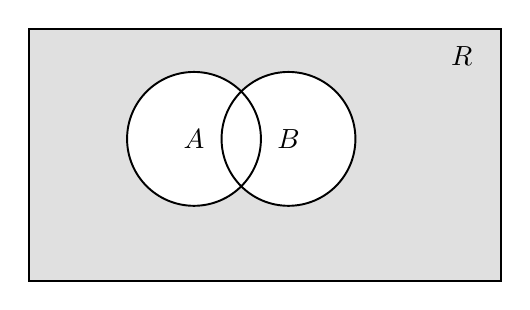
\begin{tikzpicture}[scale=1,line width=0.7pt]
\fill[black!12] (0,0) rectangle (6,3.2);
\fill[white] (2.1,1.8) circle (0.85);
\fill[white] (3.3,1.8) circle (0.85);
\draw (0,0) rectangle (6,3.2);
\draw (2.1,1.8) circle (0.85);
\draw (3.3,1.8) circle (0.85);
\node at (2.1,1.8) {$A$};
\node at (3.3,1.8) {$B$};
\node at (5.5,2.85) {$R$};
\end{tikzpicture}
\end{center}

（1）若集合 $C$ 表示图中阴影部分，用集合的运算式表示 $C$.

（2）求集合 $C$.

\ansspace*[12]

\ifanswer
\solbegin
\stepm{（1）}{由韦恩图得 $C=\overline{A\cup B}$.}
\stepm{（2）}{解 $\dfrac{x+1}{x-2}<-1$，则 $\dfrac{x+1}{x-2}+1<0$，即 $\dfrac{2x-1}{x-2}<0$，解得 $\dfrac12<x<2$，}
\step{故 $B=\left\{x\left|\dfrac12<x<2\right.\right\}$，所以 $A\cup B=\{x\mid-3\leqslant x<2\}$，}
\step{所以 $C=\overline{A\cup B}=\{x\mid x<-3\ \text{或}\ x\geqslant2\}$.}
\solend
\fi

\item 已知集合 $A=\{x\mid x^2-6x+8<0\}$，集合 $B=\{x\mid3m<x<1-m\}$.

（1）命题 $p:x\in A$，命题 $q:x\in B$，若 $p$ 是 $q$ 的充分条件，求实数 $m$ 的取值范围.

（2）若 $A\cap B=\varnothing$，求实数 $m$ 的取值范围.

\ansspace*[12]

\ifanswer
\solbegin
\stepm{（1）}{$x^2-6x+8<0\Rightarrow2<x<4\Rightarrow A=\{x\mid2<x<4\}$.}
\step{若 $p$ 是 $q$ 的充分条件，则 $A\subseteq B$，结合 $B$ 为非空集合，得 $\begin{cases}3m<1-m\\ 3m\leqslant2\\ 1-m\geqslant4\end{cases}$，}
\step{解得 $m\leqslant-3$，故 $m$ 的取值范围是 $(-\infty,-3]$；}
\stepm{（2）}{当 $B=\varnothing$ 时，$3m\geqslant1-m$，解得 $m\geqslant\dfrac14$，满足 $A\cap B=\varnothing$；}
\step{当 $B\neq\varnothing$ 时，$3m<1-m$ 即 $m<\dfrac14$，}
\step{要使交集为空，则 $1-m\leqslant2$ 或 $3m\geqslant4$，解得 $m\geqslant-1$，}
\step{结合 $m<\dfrac14$，得 $-1\leqslant m<\dfrac14$.}
\step{综上，$m\geqslant-1$，即 $m$ 的取值范围是 $[-1,+\infty)$.}
\solend
\fi

\item 设某企业每月生产电机 $x$ 台，根据企业月度报表知，每月总产值 $m$（万元）与总支出 $n$（万元）近似地满足下列关系：$m=\dfrac92x-\dfrac14$，$n=-\dfrac14x^2+5x+\dfrac74$，当 $m-n\geqslant0$ 时，称不亏损企业；当 $m-n<0$ 时，称亏损企业，且 $n-m$ 为亏损额.

（1）企业要成为不亏损企业，每月至少要生产多少台电机？

（2）当月总产值为多少时，企业亏损最严重，最大亏损额为多少？

\ansspace*[12]

\ifanswer
\solbegin
\stepm{（1）}{由题意得 $m-n\geqslant0$，即 $\dfrac92x-\dfrac14\geqslant-\dfrac14x^2+5x+\dfrac74$，}
\step{整理得 $x^2-2x-8\geqslant0$，解得 $x\geqslant4$ 或 $x\leqslant-2$（舍），}
\step{所以企业要成为不亏损企业，每月至少要生产 $4$ 台电机；}
\stepm{（2）}{由（1）得当 $0<x<4$ 时企业亏损，}
\step{亏损额 $n-m=\left(-\dfrac14x^2+5x+\dfrac74\right)-\left(\dfrac92x-\dfrac14\right)=-\dfrac14(x-1)^2+\dfrac94$，}
\step{所以当 $x=1$ 时，$n-m$ 取最大值 $\dfrac94$，}
\step{答：当月总产值为 $1$ 台时，企业亏损最严重，最大亏损额为 $\dfrac94$ 万元.}
\solend
\fi

\item 已知 $x_1$、$x_2$ 是一元二次方程 $4kx^2-4kx+k+1=0(k\neq0)$ 的两个实数根.

（1）是否存在实数 $k$，使 $x_1^2+x_2^2=\dfrac14$ 成立？若存在，求出 $k$ 的值，若不存在，请说明理由；

（2）是否存在整数 $k$，使 $\dfrac{x_1}{x_2}+\dfrac{x_2}{x_1}-2$ 的值为整数？若存在，求出 $k$ 的值，若不存在，请说明理由.

\ansspace*[14]

\ifanswer
\solbegin
\stepm{（1）}{因为 $x_1$、$x_2$ 是一元二次方程 $4kx^2-4kx+k+1=0(k\neq0)$ 的两个实数根，}
\step{所以 $\Delta=(-4k)^2-4\times4k(k+1)\geqslant0$，解得 $k\leqslant0$，}
\step{由韦达定理得 $\begin{cases}x_1+x_2=1\\ x_1x_2=\dfrac{k+1}{4k}\end{cases}$，}
\step{则 $x_1^2+x_2^2=(x_1+x_2)^2-2x_1x_2=\dfrac14$，}
\step{即 $1-2\times\dfrac{k+1}{4k}=\dfrac14$，解得 $k=2$，因为 $k\leqslant0$，所以不存在实数 $k$.}
\stepm{（2）}{$\dfrac{x_1}{x_2}+\dfrac{x_2}{x_1}-2=\dfrac{x_1^2+x_2^2}{x_1x_2}-2=\dfrac{(x_1+x_2)^2-2x_1x_2}{x_1x_2}-2=\dfrac{(x_1+x_2)^2}{x_1x_2}-4$}
\step{$=\dfrac{1}{\dfrac{k+1}{4k}}-4=\dfrac{4k}{k+1}-4=\dfrac{4k-4(k+1)}{k+1}=\dfrac{-4}{k+1}$，}
\step{由于 $\dfrac{x_1}{x_2}+\dfrac{x_2}{x_1}-2$ 的值为整数，即 $\dfrac{-4}{k+1}$ 的值为整数，}
\step{所以 $k+1$ 只能取 $\pm1$、$\pm2$、$\pm4$，}
\step{又 $k\leqslant0$，所以当 $k+1=\pm1$ 时，得出 $k=0$（舍）或 $k=-2$，}
\step{当 $k+1=\pm2$ 时，得出 $k=1$（舍）或 $k=-3$，}
\step{当 $k+1=\pm4$ 时，得出 $k=3$（舍）或 $k=-5$，}
\step{综上所述，若 $\dfrac{x_1}{x_2}+\dfrac{x_2}{x_1}-2$ 的值为整数，则 $k$ 的值为 $-2$ 或 $-3$ 或 $-5$.}
\solend
\fi

\item 已知集合 $A=\{a_1,a_2,\cdots,a_n\}(n\geqslant3)$，其中 $a_m\in\Z(m=1,2,\cdots,n)$. 若 $A$ 的子集 $T=\{a_i,a_j,a_k\}$ 满足 $2a_k=a_i+a_j$，则称 $T$ 具有性质 $P$. $A$ 的所有具有性质 $P$ 的子集 $T$ 的个数记为 $card_A(T)$.

（1）当 $A=\{4,-1,-2,1,-5\}$ 时，写出 $A$ 的所有具有性质 $P$ 的子集 $T$；

（2）当 $n=4$ 时，若 $a_1<a_2<a_3<a_4$，且 $card_A(T)=2$，证明：数对 $a_1$、$a_3$ 和 $a_2$、$a_4$ 中至少有一对中的两数奇偶性相同；

（3）当 $n=9$ 时，求 $card_A(T)$ 的最大值.

\ansspace*[14]

\ifanswer
\solbegin
\stepm{（1）}{集合 $A=\{4,-1,-2,1,-5\}$，元素按从小到大排列为 $-5$、$-2$、$-1$、$1$、$4$，}
\step{满足 $2a_k=a_i+a_j$ 的三元子集 $T$ 需满足其中一个元素是另外两个的平均数，}
\step{对于 $-5,-2,1$：$2\times(-2)=-4=-5+1$，满足条件，故 $T=\{-5,-2,1\}$，}
\step{对于 $-2,1,4$：$2\times1=2=-2+4$，满足条件，故 $T=\{-2,1,4\}$，}
\step{因此满足的子集有 $\{-5,-2,1\}$ 和 $\{-2,1,4\}$.}
\stepm{（2）}{假设数对 $(a_1,a_3)$ 和 $(a_2,a_4)$ 的两数奇偶性均不同，}
\step{即 $a_1$ 与 $a_3$ 一奇一偶，故 $a_1+a_3$ 为奇数，}
\step{$a_2$ 与 $a_4$ 一奇一偶，故 $a_2+a_4$ 为奇数，}
\step{集合 $A=\{a_1,a_2,a_3,a_4\}$ 的三元子集共 $\mathrm{C}_4^3=4$ 个：}
\step{$\{a_1,a_2,a_3\}$：若满足 $2a_2=a_1+a_3$，左边为偶数，右边为奇数，矛盾，故不满足；}
\step{$\{a_2,a_3,a_4\}$：若满足 $2a_3=a_2+a_4$，左边为偶数，右边为奇数，矛盾，故不满足；}
\step{$\{a_1,a_2,a_4\}$：需 $2a_2=a_1+a_4$；}
\step{$\{a_1,a_3,a_4\}$：需 $2a_3=a_1+a_4$.}
\step{若这两个子集都满足，则 $2a_2=2a_3\Rightarrow a_2=a_3$，与 $a_2<a_3$ 矛盾，}
\step{因此最多只有 $1$ 个子集满足条件，与 $card_A(T)=2$ 矛盾，故假设不成立，}
\step{即数对 $(a_1,a_3)$ 和 $(a_2,a_4)$ 中至少有一对的两数奇偶性相同.}
\stepm{（3）}{要最大化 $card_A(T)$，}
\step{集合 $A$ 应包含尽可能多的三元等差数列（即长度为 $3$ 的等差数列），}
\step{当 $A$ 为公差为 $1$ 的等差数列（如 $A=\{0,1,2,\cdots,8\}$）时，}
\step{三元等差数列的个数最多，}
\step{对于集合 $\{0,1,2,\cdots,8\}$，计算三元等差数列个数：}
\step{公差 $d=1$：$\{0,1,2\},\{1,2,3\},\cdots,\{6,7,8\}$，共 $7$ 个；}
\step{公差 $d=2$：$\{0,2,4\},\{1,3,5\},\cdots,\{4,6,8\}$，共 $5$ 个；}
\step{公差 $d=3$：$\{0,3,6\},\{1,4,7\},\{2,5,8\}$，共 $3$ 个；}
\step{公差 $d=4$：$\{0,4,8\}$，共 $1$ 个；}
\step{总个数为 $7+5+3+1=16$.}
\solend
\fi

\end{enumerate}

\end{document}
